%% To compile use xelatex (or lualatex):
%%   xelatex thesis-tutorial--pre-PH-fork.tex

%% 浮水印: To add watermark, compile with:
%%   xelatex '\def\addWatermark{}%% To compile use xelatex (or lualatex):
%%   xelatex thesis-tutorial--pre-PH-fork.tex

%% 浮水印: To add watermark, compile with:
%%   xelatex '\def\addWatermark{}%% To compile use xelatex (or lualatex):
%%   xelatex thesis-tutorial--pre-PH-fork.tex

%% 浮水印: To add watermark, compile with:
%%   xelatex '\def\addWatermark{}%% To compile use xelatex (or lualatex):
%%   xelatex thesis-tutorial--pre-PH-fork.tex

%% 浮水印: To add watermark, compile with:
%%   xelatex '\def\addWatermark{}\input{thesis-tutorial--pre-PH-fork.tex}'

%% To update bibliography use bibtex (or biber):
%%   bibtex thesis-tutorial--pre-PH-fork

\input{template/configure}
\begin{document}
% ------------------------------------------------
%
%論文內容次序:
% 1.考試合格證明
% 2.中英文摘要(論文以中文撰寫者須附英文延伸摘要)
% 3.誌謝
% 4.目錄
% 5.表目錄
% 6.圖目錄
% 7.符號
% 8.主文
% 9.參考文獻
% 10.附錄
%
% 註: 參考文獻書寫注意事項:
% (1).
%    文學院之中文文獻依分類及年代順序排列。
%    其他學院所之文獻依英文姓氏第一個字母
%    (或中文姓氏第一個字筆劃)及年代順序排列。
%
% (2).
%    期刊文獻之書寫依序為:
%        姓名、文章名稱、期刊名、卷別、期別、頁別、年代。
%
% (3).
%    書寫之文獻依序為:
%        姓名、書名、出版商名、出版地、頁別、年代。
%
% ------------------------------------------------


% 封面內頁 Inner Cover
%
% 封面: 顯示所有封面內容, 但沒有學校Logo)
%     主要用在印刷版, 如精裝版 或 平裝版
%     (使用cover.tex來產生)
%
% 內頁: 顯示所有封面內容, 但有學校Logo
%     主要用在電子版 + 印刷版
%
% 只要是印刷版, 不論是精裝版或平裝版, 都是 封面 (殼/皮) + 內頁.
% 只有在電子版時, 第一頁就是封面內頁.
\DisplayInnerCover

% ------------------------------------------------

% 學位考試論文證明書
\DisplayOral


% ------------------------------------------------
% 摘要 Abstract
% 除了外籍生, 本地生和僑生都是要編寫中文和英文摘要
% 論文以中文撰寫須以英文補寫 800 至 1200 字數的英文延伸摘要 (Extended Abstract)
% 詳細可看附件的學校要求或看example中的英文延伸摘要

\input{tutorial--pre-PH-fork/abstract/abstract-chi--pre-PH-fork}  % 中文版
\input{tutorial--pre-PH-fork/abstract/abstract-eng--pre-PH-fork}  % 英文版
%\input{./context/abstract/extended}        % 英文延伸摘要


% ------------------------------------------------
% 誌謝 Acknowledgments
% 誌謝正常應該只要寫一種版本就可,
% 提供2種以自行選擇所顯示的語言.
% 2種同時編寫都是可以的.

\input{tutorial--pre-PH-fork/acknowledgments/chi}             % 中文版
%\input{tutorial--pre-PH-fork/acknowledgments/eng}             % 英文版


% ------------------------------------------------
% 目錄 (內容, 圖表和圖片) Index of contents, tables and figures.
% 內容會自動產生 The indices will generate in automate.
\DisplayIndex         % 顯示索引
\DisplayTablesIndex   % 顯示表格索引
\DisplayFiguresIndex  % 顯示圖片索引


% Nomenclature
\input{tutorial--pre-PH-fork/nomenclature/nomenclature}

% Introduction section
\input{tutorial--pre-PH-fork/introduction/introduction}

% Objective section
\input{tutorial--pre-PH-fork/objective/objective}

% How-to-use section
\input{tutorial--pre-PH-fork/how-to/use/use}

% How-to-write section
\input{tutorial--pre-PH-fork/how-to/write/write}

% Words from professors section
\input{tutorial--pre-PH-fork/words-from-professor/words-from-professor}

% 參考文獻 References
\input{tutorial--pre-PH-fork/references/references}

% 附錄 Appendix
\input{tutorial--pre-PH-fork/appendix/appendix}


% 用來對內容進行不同的設定測試用的測試頁
\input{tutorial--pre-PH-fork/content-test/content-test}


\end{document}
'

%% To update bibliography use bibtex (or biber):
%%   bibtex thesis-tutorial--pre-PH-fork

%
% This file is part of the project of
% National Cheng Kung University (NCKU) Thesis/Dissertation Template in LaTex.
% This project is hold at
%     <https://github.com/wengan-li/ncku-thesis-template-latex>
% by Wen-Gan Li.
%
% This project is distributed in the hope of usefuling to someone,
% you can redistribute it and/or modify it under the terms of the
% Attribution-NonCommercial-ShareAlike 4.0 International.
%
% You should have received a copy of the
% Attribution-NonCommercial-ShareAlike 4.0 International
% along with this project.
% If not, see <http://creativecommons.org/licenses/by-nc-sa/4.0/legalcode.txt>.
%
% Please feel free to fork it, modify it, and try it.
% Have fun !!!
%

% ------------------------------------------------

\documentclass[12pt, a4paper, onecolumn, english]{report}

% ------------------------------------------------

% XeLaTex檢查點, 以要求必須使用XeLaTex來處理模版
\usepackage{ifxetex}
\ifxetex\else\errmessage{模版: 請使用XeLaTex來產生論文.}\stop\fi

% ------------------------------------------------

% 引用字體的基本設定
%
% No longer need \usepackage[T1]{fontenc} and
% \usepackage[utf8]{inputenc} when using XeLaTeX and LuaLaTeX as the engine.
%

% 引用fontspec以提供控制英文字型
\usepackage{fontspec}
\defaultfontfeatures{Ligatures=TeX} % To support LaTeX quoting style

% 引用xeCJK以提供控制中文字型
\usepackage{xeCJK}

% ------------------------------------------------

% 引用需要的LaTex packages

% Some base packages
\usepackage{geometry}
\usepackage{fp}
\usepackage{ifthen}
\usepackage{pgfkeys}
\usepackage{xparse}
\usepackage{amsmath}
\usepackage[framemethod=tikz]{mdframed}
\usepackage{url}
\usepackage{color}
\usepackage{etoolbox}

% For floats
% flafter package will make sure that the floats are
% not placed before their definition
\usepackage{flafter}

% For list
% Ref: <http://ftp.yzu.edu.tw/CTAN/macros/latex/contrib/enumitem/enumitem.pdf>
%\usepackage{enumitem}
%\setlist{noitemsep, nosep}

% For paragraphs
\usepackage{parskip}

% For line spacing
% Ref: <https://en.wikibooks.org/wiki/LaTeX/Paragraph_Formatting>
\usepackage{setspace}

% For PDF
\usepackage{hyperref}
\usepackage{pdfpages}

% For figure
\usepackage{graphicx}
\usepackage{caption}
\usepackage{subcaption}

% For table
\usepackage{array}
\usepackage{multirow}
\usepackage{booktabs}
\usepackage{diagbox}

% For comment
\usepackage{comment}

% For 目錄
\usepackage[tocgraduated]{./template/tocstyle}
\usetocstyle{standard}
%\setcounter{tocdepth}{4} % 目錄會顯示subsubsection

% For chinese number in title
% http://ftp.yzu.edu.tw/CTAN/macros/latex/contrib/zhnumber/zhnumber.pdf
\usepackage{zhnumber}

% For pseudocode
\usepackage{algorithm}
\usepackage[noend]{algpseudocode}
\algnewcommand\algorithmicswitch{\textbf{switch}}
\algnewcommand\algorithmiccase{\textbf{case}}
\algnewcommand\algorithmicdefault{\textbf{default}}
\algnewcommand\algorithmicbreak{\textbf{break}}
\algdef{SE}[SWITCH]{Switch}{EndSwitch}[1]{\algorithmicswitch\ #1\ }{\algorithmicend\ \algorithmicswitch}%
\algdef{SE}[CASE]{Case}{EndCase}[1]{\algorithmiccase\ #1:}{\algorithmicend\ \algorithmiccase}%
\algdef{SE}[CASE]{Default}{EndDefault}[0]{\algorithmicdefault:}{\algorithmicend\ \algorithmiccase}%
\algtext*{EndSwitch}%
\algtext*{EndCase}%
\algtext*{EndDefault}%
\def\Break{\algorithmicbreak}

% For theorem
\usepackage{amsthm}
\usepackage{amssymb}


% ------------------------------------------------

% 有關學校對論文要求的設定

% --------------------------

% 一些用來設定function和variable的command
\input{./template/command/command}

% --------------------------

% 學校排版 Arrangement style
\input{./template/style/style}

% --------------------------

% 論文有關資料
%%BEG content that was in input from conf/conf.tex

\ifdefined\optDOI
\usepackage{draftwatermark-2x}%  -2x indicates legacy outdated version.
% --- DOI 碼 ---
% 由2018年下學期時, 論文需要插入DOI碼顯示在右下方. DOI碼會在國立成功大學論文上傳系統中, 在上傳時提供.
% 但是2021以後,好像規定又便了。學生不必自己插入DOI碼. PH20210823
\SetWatermarkText{\textbf{doi:10.6844/ncku.latex.template.2019.Z00}}%% <--- DOI number
\SetWatermarkColor{black}
\SetWatermarkFontSize{0.5cm}
\SetWatermarkScale{0.58}
\SetWatermarkAngle{0}
\SetWatermarkLightness{0}
\SetWatermarkHorCenter{18cm}
\SetWatermarkVerCenter{28.4cm}
\fi


% ----------------------------------------------------------------------------

% --- 行距 ---
% 同學可自行設定每行的距離, 這邊是以放大縮小方式來使用.
% 所以是輸入 0.1, 0.5, 1, 1.0, 1.5, 2.0, 2 等數字.
% 預設的行距: 1.2

%\SetLineStretch{1.2}

% ----------------------------------------------------------------------------

% --- 封面上語言和名字顯示方式 ---
%
% \DisplayCoverInChi:  封面以全中文顯示
% \DisplayCoverInEng:  封面以全英文顯示
% 只能選擇其中一個, 但只有最後設定的一方有效
% 預設使用\DisplayCoverInEng
%
% 另外預設在封面上只會顯示中文或英文名字而已.
% 不論你是使用\DisplayCoverInChi或\DisplayCoverInEng,
% 使用\DisplayCoverPeoplesBothNames以設定同時顯示中英文名字.

\DisplayCoverInChi
\DisplayCoverInEng
\DisplayCoverPeoplesBothNames

% ----------------------------------------------------------------------------

% --- Draft 初稿 ---
% 顯示 '(初稿)' (中文版) 和 '(Draft)' (英文版) 在封面
\DisplayDraft

% ----------------------------------------------------------------------------

% ----------------------------------------------------------------------------

% --- Date 日期 ---

% 封面日期是統一使用學位考試合格(口試合格單)單為主要參考日期 (年、月(學位考試通過日期)).
% 例如105年7月口試,則封面日期為 中華民國105年7月 或 2016年7月.

% --- 口試的日期 ---
% 設定西元的年月日, 會自動計算出民國的年份, 和英文的月份轉換
% 次序: {年份}{月份}{日}
% \SetOralDate{2016}{12}{31}

\SetOralDate{2019}{12}{31}

%--------------------------------------------------

% --- 論文封面上的日期 ---

% 如是你是國立成功大學的學生, 則封面日期直接使用口試日期, 故不需再另設定.
% 但如果你不是國立成功大學的學生, 那本模版則不清楚 貴學校所定的規範是否要分開, 故先保留這功能.

% 設定西元的年月, 會自動計算出民國的年份, 和英文的月份轉換
% 次序: {年份}{月份}
% \SetCoverDate{2019}{12}

\SetCoverDate{2019}{12}

% ----------------------------------------------------------------------------

% --- 系所 Department or Institute ---
%
% 設定你的系所名字, e.g:
% \SetDeptMath 數學系
% \SetDeptCSIE 資訊工程學系

\SetDeptCSIE

% ----------------------------------------------------------------------------

% --- 指導老師 Advisor(s) ---
% 在封面上預算了最多3位的空間
% 中文名字固定以 博士  為結尾
% 英文名字固定以 Dr. 為開頭

% 有3種可使用, 用來設定3位老師的名字
% \SetAdvisorNameX{老師的名字}{Professor's name} % 同時設定中英文名字
% \SetAdvisorChiNameX{老師的名字}                % 只設定中文名字
% \SetAdvisorEngNameX{Professor's name}         % 只設定英文名字
% (NameX為NameA, NameB, NameC)

% 使用\SetAdvisorNameA是必須的, 而如果你的指導教授有2或3位,
% 那只要增加\SetAdvisorNameB和\SetAdvisorNameC則可

%% \SetAdvisorNameA{A}{A}
%% \SetAdvisorNameB{B}{B}
%% \SetAdvisorNameC{C}{C}

% ----------------------------------------------------------------------------

% --- 學位考試論文證明書 Defense Certificate ---
% 使用範例版本 或 使用檔案 只能選擇其中一方

% 使用範例版本
\DisplayOralTemplate

% --- 範例版本的語言 ---
% 選擇你需要的範例
% (Only work with \DisplayOralTemplate)
% \DisplayOralChiTemplate    % 顯示中文範例版本
% \DisplayOralEngTemplate    % 顯示英文範例版本

\DisplayOralChiTemplate    % 顯示中文範例版本
\DisplayOralEngTemplate    % 顯示英文範例版本

% --- 口試委員 Committee member(s) ---
% 口試委員數量 (至少2位, 最多9位, 預設為9位)
% (Only work with \DisplayOralTemplate)
% 博士學位考試委員會置委員五人至九人
% 碩士學位考試委員會置委員三人至五人
% 口試委員人數含指導教授
\SetCommitteeSize{9}

%--------------------------------------------------

% 使用學位考試論文證明書圖片檔案
% 把你的圖片放在'context/oral'下
% 之後設定中英文版所對應是哪一個檔案
% 就算已啟用\DisplayOralImage,
% 但沒有填寫圖檔檔名的話, 都不會顯示出來.
% (例子用的'example-oral-chi.pdf'和'example-oral-eng.pdf'已放在'context/oral'中)

%\DisplayOralImage                % 顯示圖檔
%\SetOralImageChi{example-oral-chi.pdf}   % 中文版檔案
%\SetOralImageEng{example-oral-eng.pdf}   % 英文版檔案

% ----------------------------------------------------------------------------

% --- 關鍵字 Keyword ---
% 最多9個關鍵字
% 為了方便同學自行設定
% 故所產出來的PDF檔案中的關鍵字和內文摘要的關鍵字
% 可獨立個別設定

% \SetKeywords是設定所產出來的PDF中的Keyword項目
% 可同時填寫中英文
% e.g
% \SetKeywords{Keyword A (關鍵字 A)}{Keyword B (關鍵字 B)}{Keyword C (關鍵字 C)}
% 或單純中文或英文
% \SetKeywords{Keyword A}{Keyword B}{Keyword C}
% \SetKeywords{關鍵字 A}{關鍵字 B}{關鍵字 C}

\SetKeywords{NCKU Thesis/Dissertation template}{Graduate}{LaTex/XeLaTex}

% 摘要中的關鍵字
% 為了方便同學們能達到以下情況:
% a. 只寫中文版摘要
% b. 只寫英文版摘要
% c. 同時寫中英文版摘要
% 故中英文版的關鍵字都是可個別設定
% \SetAbstractChiKeywords: 用來設定中文版摘要的關鍵字
% \SetAbstractEngKeywords: 用來設定英文版摘要的關鍵字
% \SetAbstractExtKeywords: 用來設定英文延伸摘要的關鍵字 (只有你要編寫英文延伸摘要才需要設定)
% 所以只要使用你需要寫的版本則可.
% 但如果2個版本都要寫, 則2個都同時使用則可.
% 沒有填寫的話, 則摘要中的關鍵字部份是不會顯示出來.
%
% e.g
% \SetAbstractChiKeywords{關鍵字 A}{關鍵字 B}{關鍵字 C}
% \SetAbstractEngKeywords{Keyword A}{Keyword B}{Keyword C}
% \SetAbstractExtKeywords{Keyword A}{Keyword B}{Keyword C}
% 英文延伸摘要的關鍵字理應會跟英文版摘要的關鍵字是一樣,
% 但為了同學能編寫不同內容和關鍵字, 故可獨立設定.

\SetAbstractChiKeywords{國立成功大學畢業論文模版}{碩博士}{LaTex/XeLaTex}
\SetAbstractEngKeywords{NCKU Thesis/Dissertation Template}{Graduate}{LaTex/XeLaTex}
\SetAbstractExtKeywords{NCKU Thesis/Dissertation Template}{Graduate}{LaTex/XeLaTex}


% --- 目錄 Index ---
% 設定可獨立使用, 但只有最後設定的一方有效

% 標題文字語言 Language
% 目錄的標題文字使用預設的中文或是英文
% \IndexChiMode:  標題文字為中文
% \IndexEngMode:  標題文字為英文
% 預設的目錄標題為: 目錄 (中文) / Table of Contents (英文)
% 預設的表格目錄標題為: 表格 (中文) / List of Tables (英文)
% 預設的圖片目錄標題為: 圖片 (中文) / List of Figures (英文)
% 預設使用\IndexEngMode

%\IndexChiMode
\IndexEngMode

% Section (節)
\SetNumberingFormat[Section]{%
  BeginText = {}, EndText = {},
  TextAlign = {Left},
  CNumStyle = {}, SNumStyle = {},
  SepAtIndex = {}, SepBetweenCnS = {},
} % End of \SetNumberingFormat{}

% SubSection (小節)
\SetNumberingFormat[SubSection]{%
  BeginText = {}, EndText = {},
  TextAlign = {Left},
  CNumStyle = {}, SNumStyle = {}, SSNumStyle = {},
  SepAtIndex = {.}, SepBetweenCnS = {}, SepBetweenSnSS = {},
} % End of \SetNumberingFormat{}
%%END content that was in input from conf/conf.tex


% --------------------------
% 在 pdf 簡介欄裡填入相關資料
\FillInPDFData

% ------------------------------------------------

% 一些會受到conf.tex中設定而影響的package或排版的設定

% Makes all pages the height of the text on that page.
% No extra vertical space is added.
%\raggedbottom

% Setup all custom numbering format
\SetupNumberingFormat

% 當所有的package都include完後, 才真正設定我們要的字型,
% 以清掉所有由package影響到的設定.
\InitDefaultFontType

%\setlength{\parindent}{4em}
%\usepackage{indentfirst}

% Initinal all theorem formats
\InitTheoremFormats

% ------------------------------------------------

% For IEEEtran
% Remove '%' to use bibliography IEEEtran style 

% \usepackage{cite}
% \renewcommand{\citedash}{--}
% \renewcommand{\citepunct}{,}

% ------------------------------------------------

\begin{document}
% ------------------------------------------------
%
%論文內容次序:
% 1.考試合格證明
% 2.中英文摘要(論文以中文撰寫者須附英文延伸摘要)
% 3.誌謝
% 4.目錄
% 5.表目錄
% 6.圖目錄
% 7.符號
% 8.主文
% 9.參考文獻
% 10.附錄
%
% 註: 參考文獻書寫注意事項:
% (1).
%    文學院之中文文獻依分類及年代順序排列。
%    其他學院所之文獻依英文姓氏第一個字母
%    (或中文姓氏第一個字筆劃)及年代順序排列。
%
% (2).
%    期刊文獻之書寫依序為:
%        姓名、文章名稱、期刊名、卷別、期別、頁別、年代。
%
% (3).
%    書寫之文獻依序為:
%        姓名、書名、出版商名、出版地、頁別、年代。
%
% ------------------------------------------------


% 封面內頁 Inner Cover
%
% 封面: 顯示所有封面內容, 但沒有學校Logo)
%     主要用在印刷版, 如精裝版 或 平裝版
%     (使用cover.tex來產生)
%
% 內頁: 顯示所有封面內容, 但有學校Logo
%     主要用在電子版 + 印刷版
%
% 只要是印刷版, 不論是精裝版或平裝版, 都是 封面 (殼/皮) + 內頁.
% 只有在電子版時, 第一頁就是封面內頁.
\DisplayInnerCover

% ------------------------------------------------

% 學位考試論文證明書
\DisplayOral


% ------------------------------------------------
% 摘要 Abstract
% 除了外籍生, 本地生和僑生都是要編寫中文和英文摘要
% 論文以中文撰寫須以英文補寫 800 至 1200 字數的英文延伸摘要 (Extended Abstract)
% 詳細可看附件的學校要求或看example中的英文延伸摘要

% ------------------------------------------------
\StartAbstractChi
% ------------------------------------------------

這是國立成功大學碩博士用畢業論文的LaTex模版. 這模版是使用學校最新的畢業論文要求來設計(參考: 附錄 - 撰寫論文須知 P.\RefPage{appendix:thesis-spec}).

這模版的目標是為了提供學生可以使用LaTex來寫畢業論文. 但是各系所有各自的格式, 故請在使用前先留意自己的系所有沒有格式要求 (參考: 附錄 - 可使用的系所 P.\RefPage{appendix:acceptable-dept}). 如果沒有, 則這模版應該用來使用; 否則要看系所上的格式, 是否跟這模版有相同的寫法.

這模版的內容是我參考了我所拿到的一些畢業論文的LaTex模版設計, 跟系上老師的一些對話, 和上課所聽得出的結論和想法而寫出的, 所以某些地方會帶有我們濃郁的資工系味道. 另外如果有任何的老師 (不論本系外系)可以提供一些意見或想法的話, 我會十分感謝的.

這模版盡量以全自動化方式去處理一些不用你去煩惱的部份, 如排版和設計. 只留下要你去填寫的部份, 所以只要選擇和填入你的內容, 就能得到一份符合學校要求的畢業論文.

最後, 希望你使用愉快.

% ------------------------------------------------
% 如果在conf.tex中的\SetAbstractChiKeywords有設定任何的關鍵字,
% 那中文版的關鍵字會在使用\EndAbstractChi後同時顯示出來.
\EndAbstractChi
% ------------------------------------------------
  % 中文版
% ------------------------------------------------
\StartAbstract
% ------------------------------------------------

Write your abstract here.

Enjoy this template.

% ------------------------------------------------
% 如果在conf.tex中的\SetAbstractEngKeywords有設定任何的關鍵字,
% 那英文版的關鍵字會在使用\EndAbstract後同時顯示出來.
\EndAbstract
% ------------------------------------------------
  % 英文版
%% ------------------------------------------------
\StartExtendedAbstract
% ------------------------------------------------

\ExtAbstractSummary{%
The summary is a short, informative abstract of no more than 250 words. References should not be cited. The summary should (1) state the scope and objectives of the research, (2) describe the methods used, (3) summarize the results, and (4) state the principal conclusions. Text of the summary should be 12 pt Times New Roman font, single-spaced and justified. A single line space should be left below the title `SUMMARY'. Leave a single line space above the key words listed below.
} % End of \ExtAbstractSummary{}

% ------------------------------------------------

\ExtAbstractChapter{INTRODUCTION}
The purpose of the introduction is to tell readers why they should want to read your thesis/ dissertation. This section should provide sufficient background information to allow readers to understand and evaluate the paper's results.

The introduction should (1) present the nature and scope of the problem, (2) review related literature, (3) describe the materials used and method(s) of the study, and (4) describe the main results of the study.

All text in the main body of the extended abstract should be 12 pt Times New Roman font, single-spaced and justified. Main headings are placed in the centre of the column, in capital letters using 12 pt Times New Roman Bold font. Subheadings are placed on the left margin of the column and are typed in 12 pt Times New Roman Bold font.

% ------------------------------------------------

\ExtAbstractChapter{MATERIALS AND METHODS}
There is flexibility as to the naming of the section (or sections) that provide information on the method(s) or theories employed. The methodology employed inthe work must be described in sufficient detail or with sufficient references so that the results could be duplicated.

Your materials should be organised carefully. Include all the data necessary to support your conclusions, but exclude redundant or unnecessary data.

% ------------------------------------------------

\ExtAbstractChapter{RESULTS AND DISCUSSION}
The results and discussion sections present your research findings and your analysis of those findings. The results of experiments can be presented as tables or figures.

% ------------------------------------------------

\ExtAbstractSection{Figures and Tables}
Figures may be integrated within the results section of the extended abstract, or they can be appended to the end of the written text. Figures should be black \& white. They should be no wider than the width of the A4 page.

Tables can be created within Word. As noted for figures above, if a table is to be placed within the text, it can be no wider than the width of the A4 page. Larger tables will need to be placed at the end of the abstract.

Figures and tables should be numbered according to the order they are referenced in the paper. Figures and tables should be referred to by their number in the text. When referring to figures and tables in the text, spell out and capitalize the word Figure or Table. All figures and tables must have captions.

% ------------------------------------------------

\ExtAbstractSection{Captions}
Captions should clearly explain the significance of the figure or table without reference to the text. Details in captions should not be restated in the text. Parameters in figure captions should be included and presented in words rather than symbols.

Captions should be placed directly above the relevant table and beneath the relevant figure. The caption should be typed in 12 pt Times New Roman Bold font. Spell out the word `Table' or `Figure' in full. An example table and a figure follow.

% ------------------------------------------------

\InsertTable
  [caption={Specifications of the engine}]
  {
    \begin{tabular}{llll}
    \hline
    Engine &  &  & OPEL Astra C16SE \\ \hline
    Displacement (cc) &  &  & 1598 \\
    Bore x stroke(mm x mm) &  &  & 79 x 81.5 \\
    Value mechanism &  &  & SOHC \\
    Number of valves &  &  & Intake 4, exhaust 4 \\
    Compression ratio &  &  & 9.8:1 \\
    Torque &  &  & 135/3400 Nm/rpm \\
    Power &  &  & 74/5800 kW/rpm \\
    Ignition sequence &  &  & 1-3-4-2 \\
    Spark plug &  &  & BPR6ES \\
    Fuel &  &  & 95 unleaded gasoline \\
    Cylinder arrangment &  &  & In-line 4 cylinders \\ \hline
    \end{tabular}
  } % End of  \InsertTable{}

\InsertFigure
  [scale=0.5,
    caption={HC emission as a function of equivalence ratio}]
  {tutorial--pre-PH-fork/abstract/pic/extended-abstract-2.jpg}

% ------------------------------------------------

\ExtAbstractChapter{CONCLUSION}
This section should include (1) the main points of your paper and why they are significant, (2) any exceptions to, problems with, or limitations to your argument, (3) agreements or disagreements with previously published work, (4) theoretical and practical implications of the work, and (5) conclusions drawn.

% ------------------------------------------------
\EndExtendedAbstract
% ------------------------------------------------
        % 英文延伸摘要


% ------------------------------------------------
% 誌謝 Acknowledgments
% 誌謝正常應該只要寫一種版本就可,
% 提供2種以自行選擇所顯示的語言.
% 2種同時編寫都是可以的.

% ------------------------------------------------
\StartAcknowledgmentsChi
% ------------------------------------------------

感謝同學們和老師們在不同地方上的幫忙和意見, 以讓本模板更完整, 閱讀更清楚, 有關資料已放在`CONTRIBUTE'中.

同時感謝在圖書館和教務處課務組的職員去查核本模板所產生的樣子適合當成畢業論文, 以讓同學可以安心使用本模板.

% ------------------------------------------------
\EndAcknowledgments
% ------------------------------------------------
             % 中文版
%% ------------------------------------------------
\StartAcknowledgments
% ------------------------------------------------

Thanks someone you want in here.

% ------------------------------------------------
\EndAcknowledgments
% ------------------------------------------------
             % 英文版


% ------------------------------------------------
% 目錄 (內容, 圖表和圖片) Index of contents, tables and figures.
% 內容會自動產生 The indices will generate in automate.
\DisplayIndex         % 顯示索引
\DisplayTablesIndex   % 顯示表格索引
\DisplayFiguresIndex  % 顯示圖片索引


% Nomenclature
% ------------------------------------------------
\StartSection{術語/符號 Nomenclature}{chapter:how-to:write:nomenclature}
% ------------------------------------------------

Nomenclature在定義一些在整份論文中所會用到的變數是很常用到的. 它的位置會出現在文章當中或是在Chapter 1之前. 它的設計沒有一個標準答案, 在不同的情況下可能有不同顯示方式, 但它基本上跟一張Table是沒差的. 而它在Latex中是使用一個package名為`nomencl'.

但經過研究了一下package `nomencl'或tabbing這些用來建Nomenclature的方式後, 發現`nomencl'在設計上反而會增加在產生論文時的步驟; 而tabbing要自行定義一個闊度才能弄得比較好看, 但同時內容卻出現沒法置中和設計上等一些問題. 故最後決定直接套用Table來讓同學更能自由的設計不同的Nomenclature table.

設計Nomenclature table需要2個知識或工具:\\
1) 設計一張Table, 這邊請參考P. \RefPage{chapter:how-to:write:table}.\\
2) 有關所需要用到的符號, 請參考Equation (P. \RefPage{chapter:how-to:write:equation})中所使用到的工具, Texmarker左邊的工具列, 或看這幾個網頁\RefBib{web:symbols:site1}\RefBib{web:symbols:site2}\RefBib{web:symbols:site3}, 應該已經足夠同學們寫出合適的符號.

% ------------------------------------------------
%\newpage
\StartSubSection{使用方式}

如果是指是在Chapter 1之前的一大張的Nomenclature table, 為Nomenclature Chapter.
  \begin{verbatim}
  \StartNomChapter{ NAME }{ LABEL }
  \EndNomChapter
  \end{verbatim}
Nomenclature Chapter跟一般Chapter的使用方式是一樣的, 但差別在於不會出現`Chapter'這字眼. 而由於大家的Nomenclature Chapter name可能不一樣, 故跟Chapter一樣可設定自行的name.

而如果是在文章當中的Nomenclature table. 基本上就是使用同一個的`\verb|\InsertTable|', 但還可以使用`nomtitle'來設定標題. `nomtitle'跟`caption'的差別是, 使用`nomtitle'所顯示出來的標題是沒有`Table XX:'為開頭, 同樣都是使用`pos'來控制題目的位置.

  \begin{DescriptionFrame}
  \begin{verbatim}
  Options 設定
    nomtitle:   Nomenclature 標題 (選填)
    ...

  E.g
    \InsertTable
    [nomtitle={這是Nomenclature Table的標題}]
      {
        ...
      }
  \end{verbatim}
  \end{DescriptionFrame}

有關這個的用法可參考`tutorial--pre-PH-fork/nomenclature/nomenclature.tex'中的Nomenclature Chapter所demo的例子, 那2個例子只是最簡單的Nomenclature table設計, 應該足夠同學們去弄出合適自己的Nomenclature table的設計.


% Introduction section
% ------------------------------------------------
\StartChapter{Introduction}{chapter:introduction}
% ------------------------------------------------

這是國立成功大學碩博士用畢業論文的LaTex模版. 本模版是使用學校最新的畢業論文要求來設計(參考: 附錄 - 撰寫論文須知 P.\RefPage{appendix:thesis-spec}).

雖然本模版的目標是為了提供學生可以使用LaTex來寫畢業論文. 但是各系所有各自的格式, 所以做了一個表列出已知的系所情況(參考: 附錄 - 可使用的系所 P.\RefPage{appendix:acceptable-dept}), 故請在使用前先留意自己的系所有沒有格式要求. 如果沒有, 則本模版應該是可以用來使用; 否則要看系所上的格式, 是否跟本模版有相同的寫法.

本模版分以下幾個主要部份來進行教學:

\begin{enumerate}
  \item 本模版的架構設計
  \item 設定本模版的一些資料以轉成你的論文
  \item 介紹LaTex和本模版所提供的語法
  \item 最後有一個chapter為``老師們的話''(Chap.\RefTo{chapter:words-from-professor})寫了一些老師對論文的想法和意見, 以供同學們留意
\end{enumerate}

同學們只要閱讀完後, 把部份的檔案直接copy和修改內容, 應該很快就能上手本模版去寫自己的論文.

另外在附錄(Appendix)附上了一些重要的學校的文件, 由於本模版很接近完善, 故直接使用本模版後可不需再閱過學校相關規定之文件, 所以該類文件置於此僅為備考用.

% ------------------------------------------------
\newpage

\begin{description}
  \item[版權 License]\hfill\\
  詳細請看`LICENSE'這檔案中的條款說明.\\

  \InsertFigure
    [scale=0.8,
      caption={CC Attribution-NonCommercial-ShareAlike License},
      label={fig:appendix:by-nc}]
    {./tutorial--pre-PH-fork/introduction/pic/by-nc-sa.png}

    本著作(ncku-thesis-template-latex\RefBib{web:this-project:github})採用創用 CC 姓名標示-非商業性-相同方式分享 4.0 授權條款.

    This work(ncku-thesis-template-latex\RefBib{web:this-project:github}) is licensed under Creative Commons Attribution-NonCommercial-ShareAlike 4.0 International License.\\

  而本模版所使用到的國立成功大學浮水印則由國立成功大學擁有\textbf{所有}相關的權利. 故如使用這浮水印到論文以外的應用, 請跟`成大圖書館 系統管理組-數位論文小組'聯絡.\\

  \item[版本修改 ChangeLog]\hfill\\
  詳細請看`ChangeLog.md'這檔案中的說明.
\end{description}

% ------------------------------------------------
\EndChapter
% ------------------------------------------------


% Objective section
% ------------------------------------------------
\StartChapter{Objective}{chapter:objective}
% ------------------------------------------------

\StartSection{起因}

做這個模版的原因其實很簡單:

\begin{enumerate}
  \item
  {
    去投國外paper時, 對方可能會要求使用LaTeX, 所以未來要懂LaTeX是不意外的.
  } % End of \item{}

  \item
  {
    想拿LaTeX來寫畢業論文, 卻發現學校只提供Mircosoft Word模版, 但卻沒有提供LaTeX的, 所以證明本模版對學校是有存在價值的.
  } % End of \item{}

  \item
  {
    因為看到發現台灣科技大學\RefBib{web:latex:template:ntust}, 台灣大學\RefBib{web:latex:template:ntu}, 元智大學\RefBib{web:latex:yzu}都能找到LaTeX的模版, 連大陸那邊都有一些學校有在提供, 更不用說國外的學校.

    那些學校的畢業論文模版不只提供是Mircosoft Word版本(.doc), 是會連LaTex(.tex)版本都有, 而我們學校卻沒有. 唯一我們學校在Google上找到的有提到的卻是數學系系網頁上的功能\RefBib{web:latex:ncku_math_introduction}和建在數學系上的一個討論區\RefBib{web:latex:ncku_math_forum}.
  } % End of \item{}

  \item
  {
    因為學校對Phd跟Master的畢業論文要求是同一個格式, 所以如果完成後對學校任何學生應該都有其好處.

    對大家都有多一個選擇來寫畢業論文, 而不是被限在使用Mircosoft Word來寫.
  } % End of \item{}

  \item
  {
    經過詢問我們資訊工程系(CSIE)的系上一些老師後, 意外發現原來某些實驗室其實已經有各自的版本存在, 但每個版本都有各自的優缺點, 例如:

    \begin{enumerate}

      \item
      {
        新的使用者或接手的人不容易修改或使用.
      } % End of \item{}

      \item
      {
        或是需要安裝的步驟十分麻煩 (e.g cwTeX\RefBib{web:latex:cwtex}).
      } % End of \item{}

      \item
      {
        另外有一些因為是只針對英文版本, 沒有考量在編寫或初稿時會有中英混雜的時候, 故這時候中英文的內容要分開編寫和產生 (學校又要求, 英文內容的論文要同時有中文論文名字等), 所以需要把整個論文分開成不同的檔案.
      } % End of \item{}
    \end{enumerate}
  } % End of \item{}
\end{enumerate}

% ------------------------------------------------

%\newpage
\StartSection{目標}
所以為了解決以上的問題, 這個模版針對了好幾點來處理:

\begin{enumerate}

  \item
  {
    把本模版做到連笨蛋都可以很快懂得使用(所謂的Books for Dummies), 所以只留下使用者要填寫的部份外, 其他都交由模版去負責.
  } % End of \item{}

  \item
  {
    希望做到使用者只讀這份模版, 就會懂得去修改和寫自己所需的內容(所謂的Self-contained. 但其實是不太可能的, 因為LaTex的使用手冊就算寫成一本幾百頁的書, 都可以缺少很多東西), 所以會同時提供很基本使用LaTex的方式, 和填寫本模版步驟.
  } % End of \item{}

  \item
  {
    希望一份模版, 能同時應用在中文或是英文版本, 只要修改內容和一些的設定.
  } % End of \item{}

  \item
  {
    把本模版open source, 讓以後任何的同學們都可以使用和修改, 以合適當時的需求.
  } % End of \item{}

\end{enumerate}

而選擇使用XeLaTex的原因, 是經過分析cwTeX, CJK和XeLaTex後. 發現cwTeX的寫法太糟, 要背多新一種語法, 而且安裝複雜\RefBib{web:latex:cwtex}; 而CJK有一定程度的設定才能在整個論文中自由使用, 感覺設定麻煩而不太能笨蛋化來用, 所以放棄選用; 故最後選用最簡單加一些包裝, 就可以簡單使用中英混合的XeLaTex.

% ------------------------------------------------

\StartSection{缺點}
但是同樣任何東西都會有缺點, 故本模版都不意外:

\begin{enumerate}

  \item
  {
    本模版是以台灣國立成功大學所最新訂下的畢業論文要求(參考: 附錄 - 撰寫論文須知 P.\RefPage{appendix:thesis-spec})來設計, 所以不一定能對非本校的人有用.
  } % End of \item{}

  \item
  {
    對沒有程式基礎, 只會用Mircosoft Word的人來講, 可能會在修改或使用上會十分吃力.
  } % End of \item{}

  \item
  {
    因為我針對某些使用者不用去接觸的部份, 進行了大量的包裝(Wrapping), 所以如果懂得LaTex的人可能會覺得我破壞了LaTex的語法. 但是本模版是針對笨蛋化和全自動, 我相信對不熟LaTex的人來講, 才不管這問題 (如同一般理論派和應用派的差別, 在意的方向完全不一樣).
  } % End of \item{}

%  \newpage
  \item
  {
    某些包裝出來的語法, 可能會在一些情況下會產生衝突而令LaTex不接受, 這時候有2種做法:
    \begin{enumerate}
      \item
      {
        不使用某些寫法, 例如已知的`\verb|\InsertFigure|'沒法被包在Table, minipage或framebox中.
      } % End of \item{}

      \item
      {
        如真的要使用那些情況, 那就不要使用模版提供的語法, 而直接去寫LaTex原版的語法.
      } % End of \item{}
    \end{enumerate}
  } % End of \item{}
\end{enumerate}

% ------------------------------------------------

\StartSection{總結}

以上是個人對這份模版的一些想法和起源, 同時希望本模版能對你提供到一些幫助.

% ------------------------------------------------
\EndChapter
% ------------------------------------------------


% How-to-use section
% ------------------------------------------------
\StartChapter{本模版使用教學}
% ------------------------------------------------

% Section
\input{tutorial--pre-PH-fork/how-to/use/intro/intro}
\newpage\input{tutorial--pre-PH-fork/how-to/use/source-tree}
\newpage\input{tutorial--pre-PH-fork/how-to/use/build/build}
\newpage\input{tutorial--pre-PH-fork/how-to/use/conf}

% ------------------------------------------------
\EndChapter
% ------------------------------------------------


% How-to-write section
% ------------------------------------------------
\StartChapter{LaTex編寫教學}
% ------------------------------------------------

% ------------------------------------------------
\StartSection{基本介紹 Introduction}{chapter:how-to:write:intro}
% ------------------------------------------------

這教學包含了原LaTex和本模版特有的語法的使用方式和例子. (真正完完整整的LaTex教學手冊可不只單單幾百頁的厚度, 所以減少大家的時間, 所以本模版教學只講一些幾乎大家100\%會需要使用的語法).

請注意原LaTex語法會以英文小寫來顯示(\verb|\aabbcc|); 而本模版特有的語法會以英文大小寫混合(\verb|\AaBbCc|, 第一個字必定以大寫來顯示), 由於這些特有語法\textbf{不是}原LaTex的語法, 所以不能直接應用在非本模版的LaTex檔案上.

抄襲就是學習的第一步 (如同我們小時候去抄襲父母走路一樣), 所以本模版有留下了一些範本 (在`./context'下)以方便大家開始第一步, 之後就要靠大家自己的努力和實作, 再加上自己的探索能力了.

%\newpage
有問題的話, 可以有以下的地方找尋答案 (請使用這順序):
\begin{enumerate}
  \item 請一步一步增加內容, 如發生錯誤, 就把剛剛新增的內容拿掉, 以找出錯誤的地方
  \item 直接研究在模版的LaTex寫法 (在 'example--pre-PH-fork/' 以下的所有檔案)
  \item 查問懂得LaTex的老師和同學
  \item 去LaTex的Wikibook \RefBib{web:latex:wikibooks}\\
        這邊有大量的例子, 但是這些例子都是獨立的, 所以潛在語法混合後的會發生沖突的可能性; 另外都十分推薦去讀 '大家來學LaTeX' \RefBib{web:latex:latex123}
  \item 請求Google老師
\end{enumerate}

另外, 如果覺得本教學還缺少了什麼說明, 請告知.

% ------------------------------------------------

% Section
\newpage\input{tutorial--pre-PH-fork/how-to/write/basic/basic}
\newpage\input{tutorial--pre-PH-fork/how-to/write/chapter/chapter}
\newpage\input{tutorial--pre-PH-fork/how-to/write/figure/figure}
\newpage\input{tutorial--pre-PH-fork/how-to/write/table/table}
\newpage\input{tutorial--pre-PH-fork/how-to/write/equation/equation}
\newpage\input{tutorial--pre-PH-fork/how-to/write/nomenclature/nomenclature}
\newpage\input{tutorial--pre-PH-fork/how-to/write/bib/bib}
\newpage\input{tutorial--pre-PH-fork/how-to/write/pseudocode/pseudocode}

% ------------------------------------------------
\EndChapter
% ------------------------------------------------


% Words from professors section
% ------------------------------------------------
\StartChapter{老師們的話 Words from Professors}{chapter:words-from-professor}
% ------------------------------------------------

這部份的內容節錄於我跟系上老師的一些對話, 和上課所聽得出的結論和想法而整理出來的, 所以某些地方會帶有我們濃郁的資工系味道. 另外如果有任何的老師 (不論本系外系)可以提供一些意見或想法的話, 我會十分感謝的.

% ------------------------------------------------
\StartSection{想法}

\begin{enumerate}
  \item
  {
    有用才算創新, 要站在使用者的角度去想
  } % End of \item{}

  \item
  {
    技術$\neq$研究, 是研究才有系統跟技術
  } % End of \item{}

  \item
  {
    研究
    \begin{itemize}
      \item
      {
        就是去想問題, 以不同的角度去想東西跟解決的方法
      } % End of \item{}

      \item
      {
        十分重要的是, 為什麼要這樣做, 這跟別人有什麼差別, 而且這樣做好處是什麼
      } % End of \item{}

      \item
      {
        `工程科系'是以多答案去解決一個問題, 而`理科'是提出一個標準的答案
      } % End of \item{}

      \item
      {
        不要相信直覺, 要所有東西都要證據
      } % End of \item{}

      \item
      {
        找研究題目的方法
      } % End of \item{}

      \begin{enumerate}
        \item
        {
          針對傳統的問題, 用方法不一樣去處理它
        } % End of \item{}

        \item
        {
          把一個問題的原本假設, 環境和條件之類的進行變動, 以得到不同的結果
        } % End of \item{}
      \end{enumerate}
    \end{itemize}
  } % End of \item{}

  \item
  {
    在coding中, Bug就是你的盲點或你所不懂的.

    所以如果你在debug時是位置``經驗法則''來預估bug的位置, 這即是進行while loop, 永遠都找不到.

    你首先要得到bug所經過的code, 一個一個地插入debug message來分析變數和跑到哪去, 慢慢地縮少範圍, 這樣有數據式debug, 會比``經驗法則''來得快.
  } % End of \item{}
\end{enumerate}

% ------------------------------------------------
\StartSection{投影片/presentation}

\begin{enumerate}
  \item
  {
    口試用PPT
    \begin{itemize}
      \item
      {
        要有outline, 而且要講大約要用多少時間來講
      } % End of \item{}

      \item
      {
        每個chapter都有一個頁面用來做分頁, 以讓口試委員知道聽到哪一個部份了.
      } % End of \item{}

      \item
      {
        需要一些backup slide; 例如只講5張而已, 但backup用50張; 內容主要是一些data的來源, 和名詞解釋等
      } % End of \item{}

      \item
      {
        最核心要留時間用心讀給口試委員知道, 就算慢慢講用了2-3分鐘都是非常值得的.
      } % End of \item{}

      \item
      {
        ppt每一個section都要有一頁做summary/換頁作為結尾, 以讓聽的人回憶, 記憶, 剛說了什麼.
      } % End of \item{}

      \item
      {
        如果內容是多個block的流程, 要想辦法顯示出自己在講的位置, 否則別人會幾頁後就忘了前面在說什麼.
      } % End of \item{}

      \item
      {
        如果下頁是一個demo, 畫面之類等圖案, 圖片. 在上一頁的結尾是說``下一頁會展示這東西xxxx的畫面''.
      } % End of \item{}

      \item
      {
        在ppt中, 在說明自己的方法, 如``Result - Method A'', Method A 應用斜體字.
      } % End of \item{}

    \end{itemize}
  } % End of \item{}

  \item
  {
      1分鐘的報告
    \begin{itemize}
      \item
      {
        用one slide
      } % End of \item{}

      \item
      {
        主要使用graph
      } % End of \item{}

      \item
      {
        1,2 句的text
      } % End of \item{}

      \item
      {
        Some data
      } % End of \item{}

      \item
      {
        要做得能吸引眼睛
      } % End of \item{}
    \end{itemize}
  } % End of \item{}

  \item
  {
    一般報告paper
    \begin{itemize}
      \item
      {
        報1張ppt的時間應該是只有1分鐘左右 (除非詳細的系統架構圖), 因為讀1個中文字大約0.3秒
      } % End of \item{}

      \item
      {
        總原則
        \begin{enumerate}
          \item
          {
            解決了\textbf{`什麼'}的問題, 一定要非常清楚, 簡潔有力的說明
          } % End of \item{}

          \item
          {
            多用圖, 文字要讀完才能理解, 但圖可以有一看就懂的效果
          } % End of \item{}
        \end{enumerate}
      } % End of \item{}

      \item
      {
        Introduction
        \begin{enumerate}
          \item
          {
            什麼環境
          } % End of \item{}

          \item
          {
            什麼應用而造成這個問題
          } % End of \item{}

          \item
          {
            Given什麼條件
          } % End of \item{}

          \item
          {
            Find什麼條件
          } % End of \item{}

          \item
          {
            在什麼狀態下
          } % End of \item{}

          \item
          {
            Idea of the solution\\
            把最基本的精神講出來就可以, 不需要講detail
          } % End of \item{}
        \end{enumerate}
      } % End of \item{}

      \item
      {
        Related Work
        \begin{enumerate}
          \item
          {
            講解相關的研究
          } % End of \item{}

          \item
          {
            在1x分鐘中的報告是不用講, 除非如果不講相關的研究, 接下去觀眾就會完全不懂, 這才需要去提到 (因為是非常相關)
          } % End of \item{}
        \end{enumerate}
      } % End of \item{}

      \item
      {
        演算法
        \begin{itemize}
          \item
          {
            No
            \begin{enumerate}
              \item
              {
                不要講變數
              } % End of \item{}

              \item
              {
                不要把整個演算法顯示出來一步步講
              } % End of \item{}

              \item
              {
                不要用pseudocode
              } % End of \item{}
            \end{enumerate}
          } % End of \item{}

          \item
          {
            Yes
            \begin{enumerate}
              \item
              {
                盡量使用圖片來講解演算法
              } % End of \item{}
            \end{enumerate}
          } % End of \item{}
        \end{itemize}
      } % End of \item{}

      \item
      {
        公式
        \begin{enumerate}
          \item
          {
            不用講detail\\
            $ P( Q_{ni} ) = \frac{ 2^{k} - 1}{ 2^{n} - 1} $\\
            右邊部份不用說明\\
            只要講一整個公式的用途是在算什麼就行了
          } % End of \item{}

          \item
          {
            $ REL = A + B + C $\\
            只要講$REL$在算什麼就行了\\
            (除非別人不懂在講要算什麼, 才要把A, B, C都講出來大約算什麼則行了)
          } % End of \item{}
        \end{enumerate}
      } % End of \item{}

      \item
      {
        Theorem定理
        \begin{enumerate}
          \item
          {
            Definition\\
            在以後會常常說明的觀念, 為了以後方便講解和使用, 則使用Definition.\\
            在1x分鐘的報告中, 如果不常用,則不用講Definition, 如需要或常常會使用才需要.
          } % End of \item{}

          \item
          {
            Lemma\\
            是Theorem分開用來簡單說明的一個東西
          } % End of \item{}

          \item
          {
            Theorem\\
            是Lemma集合出的一個理論
          } % End of \item{}

          \item
          {
            Corollary\\
            在Theorem的結果用另一種條件或什麼得出的另一結果
          } % End of \item{}

          \item
          {
            Proposition\\
            以上的看情況來決定要不要講, 如果是跟algorithm無關的, 則不用講, 否則要講一點點.\\

            如果不講定理, 都能講懂algorithm, 那則不用講.\\
            而如果algorithm會使用到一個小小的定理, 即只要講定理的結果.
          } % End of \item{}

          \item
          {
            Proof\\
            在報告時是絕對不用講的
          } % End of \item{}
        \end{enumerate}
      } % End of \item{}

      \item
      {
        Performance\\
        除非作者沒有提供任何做實驗的數據, 否則正常情況下都要講解這部份的內容.
        (有一些研究方向或實驗室, 沒有要求對這部份作要求的話, 那是可以不用說明的)\\
        必須說明作者使用的dataset是什麼, 環境是什麼等一些基本資料. 之後作者做了什麼實驗, 效果如何, 發現了什麼.

        但是注意的是要對內容進行選擇, 不必要100\%的實驗資料都要拿出來講解, 只要講解這演算法最核心的一些實驗(如系統架構)就可以了.
      } % End of \item{}

      \item
      {
        優缺點, 建議 (十分重要)\\
        優點其實作者就會大力的說明, 所以不難找到.\\
        但是更重要的是, 作者一般都不會點出這演算法的缺點, 所以必須要看懂缺點在哪, 有什麼建議, 有什麼可以改進的方法, 或是有什麼方法可以用來延伸.
      } % End of \item{}

      \item
      {
        總結
        \begin{enumerate}
          \item
          {
            愈快讓人明白整個paper的要點.
          } % End of \item{}

          \item
          {
            最好能用圖片來說明.
          } % End of \item{}

          \item
          {
            Top-Down manner\\
            先講整體的觀念, 後才一部份一部份的講內容
          } % End of \item{}
        \end{enumerate}
      } % End of \item{}
    \end{itemize}

    科技論文, 是一開始就把結果說出來; 而其他的作文, 則是使用`起、承、轉、合'的手法. 但這是對論文是不對的.
  } % End of \item{}
\end{enumerate}

% ------------------------------------------------
\StartSection{投論文的目標}

\begin{enumerate}
  \item
  {
    學位論文不影響以後把內容用來投去什麼的地方, 例如可以把學位論文100\%把內容移到journal中. 所以最重要的要做是優先把學位論文寫的, 才考慮投去哪
  } % End of \item{}

  \item
  {
    找paper用來投的地方, 可以到``系網->學生事務->碩博士->期刊,會議點數''
  } % End of \item{}

  \item
  {
    寫完才考慮投去哪裡, 才把資料修成那邊要的樣子
  } % End of \item{}
\end{enumerate}

% ------------------------------------------------
\StartSection{實驗的比較對象}

\begin{enumerate}
  \item
  {
    千萬不能對不同架構, 規模不一樣的對象來進行比較
  } % End of \item{}

  \item
  {
    用電腦系統來講
    \begin{itemize}
      \item
      {
        Single server只能跟single server比較
      } % End of \item{}

      \item
      {
        Distributed system只能跟distributed system來比
      } % End of \item{}
    \end{itemize}
  } % End of \item{}
\end{enumerate}

% ------------------------------------------------
\StartSection{Related work}

只要有提到的對象, 就要去跟它比較; 不能比的就要去講差別; 有paper的就要去實作別人的部份功能

% ------------------------------------------------
\StartSection{References}

\begin{enumerate}
  \item
  {
    要拿去哪投哪裡, 就起碼最少要引用一篇那邊的paper, 否則對方一般都不太想去看 (利益問題)
  } % End of \item{}

  \item
  {
    References所選的對象, 要根據這排名去選, 越高越有說服力:
    \begin{itemize}
      \item
      {
        Paper / book\\
        Paper所提出的東西一定會做過實驗或計算, 所以有一定的正確性. 但更新速度快, 所以會有很大量的.\\
        Book是經過好多年才會把一些正確的知識整合起來, 所以速度較慢, 但是以當代來講是最正確.
      } % End of \item{}

      \item
      {
        Tech report / Datasheet\\
        Tech report是一些人對某種東西去做研究或實驗, 所以他們會先把那個東西進行分析和理解, 故所寫出來的東西都經過他們的分析和研究, 雖然沒有paper那種程度的說服力, 但還是可以被人用來學習和引用的.\\
        Datasheet是一個系統或library的開發者所寫下來的, 因為他們是最懂得那東西, 所以使用他們的資料是可以被接受的.
      } % End of \item{}

      \item
      {
        Article\\
        Article是某些或某人去對一個主題去做, 所以所寫所說都是他們的立場或想法, 不一定100\%是正確; 但這些Article都是在反映人們對某主題的分析或理解, 所以可以代表以當代來講, 人們在意的部份是什麼.
      } % End of \item{}

      \item
      {
        URL / Website\\
        URL是最不應該當成References來使用, URL出現只能當符合以下情況:
        \begin{itemize}
          \item
          {
            URL所指向的是系統, tools, library的官方網站
          } % End of \item{}

          \item
          {
            URL所指向的是有關所使用的系統, tools, library的Datasheet
          } % End of \item{}

          \item
          {
            URL所指向的是Related work中要比較的對象它相關的資料會使用在這篇論文中, 如source code.
          } % End of \item{}
        \end{itemize}

        否則的話, 千萬不要放, 因為越多的URL, 說服力會越低.\\

        另外都千萬不要使用Wikipedia當成References, 雖然Wikipedia是知識解說的地方, 但Wikipedia正因為太普遍, 所以完全沒有任何特殊的說服力; 如同介紹人們去做search網頁時, 可以使用google, yahoo是同一個道理.
      } % End of \item{}
    \end{itemize}
  } % End of \item{}
\end{enumerate}

% ------------------------------------------------
\StartSection{圖上的文字 / 表格}

除非特殊要求, 否則不能比正常的文字小 (必須 $ >= $ 10 pt), 要令人感覺每一個文字都是一樣大的, 要讓讀者可以一口氣看, 而不用做放大放小的行為.

% ------------------------------------------------
\StartSection{寫作技術}

每一個新section的開頭段落, 不能以`所以', `so'等文字, 而是必須要再用一些文字當起點, 如`前一章提到xxxxxx'.

% ------------------------------------------------
\StartSection{內容}

\begin{enumerate}
  \item
  {
    Paper必須要做到self-contained, 要把用到的其他知識時, 必須要有example以解釋這thesis在說什麼
  } % End of \item{}

  \item
  {
    不能使用了別的東西, 而完全沒解釋是什麼意思, 要讀者去查References的資料去理解這thesis在做什麼
  } % End of \item{}
\end{enumerate}

% ------------------------------------------------
\StartSection{公式}

\begin{enumerate}
  \item
  {
    避免重複使用\\
    $
      \begin{array}{ll}
            P(X) = \ldots & (A)\\
            P(X) = \ldots & (B)
      \end{array}
    $\\
    但2個$ P(X) $都代表不同的意思
  } % End of \item{}

  \item
  {
    大小寫不能一起用\\
    如 $ rel (a) $, $ REL(a) $, 但是不同意思
  } % End of \item{}

  \item
  {
    Subscript/superscript\\
    上下標是用來區分用的\\
    如$ w_{1} $, $ w_{2} $, $ w_{3} $ $ \ldots $.\\

    但不需要的話, 就不要加這個東西, 如:\\
    $
      \left\{
        \begin{array}{ll}
          r_{1}(a) & = \ldots\\
          r_{2}(a) & = \ldots
      	\end{array}
      \right.
    $\\
    但2個$ r(a) $代表同一個意思
  } % End of \item{}

  \item
  {
    名字不要太長\\
    如$ sim(a,b) $\\
    因為很像similarity (相似), 所以可以使用, 但沒有近像的字, 就不要用寫這樣
  } % End of \item{}

  \item
  {
    變數沒用就不要寫\\
    如$ pv(u,a) = 1 / distance $\\
    $U$和$a$都是沒意義, 所以可以去掉
  } % End of \item{}
\end{enumerate}

% ------------------------------------------------
\EndChapter
% ------------------------------------------------


% 參考文獻 References
% References and bibliography

% Import the files that contain your references.
% If you set some references file,
% you need to use at least one cite to make LaTex work.

\ReferencesFiles{tutorial--pre-PH-fork/references/paper}{tutorial--pre-PH-fork/references/misc}{tutorial--pre-PH-fork/references/book}


% 附錄 Appendix
% ------------------------------------------------
\StartAppendix
% ------------------------------------------------

\input{tutorial--pre-PH-fork/appendix/acceptable-dept}
\input{tutorial--pre-PH-fork/appendix/submit-flow}
\input{tutorial--pre-PH-fork/appendix/thesis-spec}
\input{tutorial--pre-PH-fork/appendix/e-paper_upload}
\input{tutorial--pre-PH-fork/appendix/e-paper_upload_ppt}
\input{tutorial--pre-PH-fork/appendix/oral-notice}
\input{tutorial--pre-PH-fork/appendix/faq}
\input{tutorial--pre-PH-fork/appendix/unicode-symbols}

% ------------------------------------------------
\EndAppendix
% ------------------------------------------------



% 用來對內容進行不同的設定測試用的測試頁
% ------------------------------------------------
\StartChapter{測試頁 Testing Pages}
% ------------------------------------------------

這邊是用來放置不同的內容來進行測試或設計樣版用的.

% 半形字元與全形字元
\input{tutorial--pre-PH-fork/content-test/half-full-char}

% 英文內容
\input{tutorial--pre-PH-fork/content-test/eng-content}

% 中文內容
\input{tutorial--pre-PH-fork/content-test/chi-content}

% 混合的中英文內容
\input{tutorial--pre-PH-fork/content-test/eng-chi-mix-content}

% 表格
\input{tutorial--pre-PH-fork/content-test/table}

\input{tutorial--pre-PH-fork/content-test/figure}

\input{tutorial--pre-PH-fork/content-test/equation}

% Chapter/Section
\input{tutorial--pre-PH-fork/content-test/chapter-section}

\input{tutorial--pre-PH-fork/content-test/ref-cite}

\input{tutorial--pre-PH-fork/content-test/theorem}

% ------------------------------------------------
\EndChapter
% ------------------------------------------------



\end{document}
'

%% To update bibliography use bibtex (or biber):
%%   bibtex thesis-tutorial--pre-PH-fork

%
% This file is part of the project of
% National Cheng Kung University (NCKU) Thesis/Dissertation Template in LaTex.
% This project is hold at
%     <https://github.com/wengan-li/ncku-thesis-template-latex>
% by Wen-Gan Li.
%
% This project is distributed in the hope of usefuling to someone,
% you can redistribute it and/or modify it under the terms of the
% Attribution-NonCommercial-ShareAlike 4.0 International.
%
% You should have received a copy of the
% Attribution-NonCommercial-ShareAlike 4.0 International
% along with this project.
% If not, see <http://creativecommons.org/licenses/by-nc-sa/4.0/legalcode.txt>.
%
% Please feel free to fork it, modify it, and try it.
% Have fun !!!
%

% ------------------------------------------------

\documentclass[12pt, a4paper, onecolumn, english]{report}

% ------------------------------------------------

% XeLaTex檢查點, 以要求必須使用XeLaTex來處理模版
\usepackage{ifxetex}
\ifxetex\else\errmessage{模版: 請使用XeLaTex來產生論文.}\stop\fi

% ------------------------------------------------

% 引用字體的基本設定
%
% No longer need \usepackage[T1]{fontenc} and
% \usepackage[utf8]{inputenc} when using XeLaTeX and LuaLaTeX as the engine.
%

% 引用fontspec以提供控制英文字型
\usepackage{fontspec}
\defaultfontfeatures{Ligatures=TeX} % To support LaTeX quoting style

% 引用xeCJK以提供控制中文字型
\usepackage{xeCJK}

% ------------------------------------------------

% 引用需要的LaTex packages

% Some base packages
\usepackage{geometry}
\usepackage{fp}
\usepackage{ifthen}
\usepackage{pgfkeys}
\usepackage{xparse}
\usepackage{amsmath}
\usepackage[framemethod=tikz]{mdframed}
\usepackage{url}
\usepackage{color}
\usepackage{etoolbox}

% For floats
% flafter package will make sure that the floats are
% not placed before their definition
\usepackage{flafter}

% For list
% Ref: <http://ftp.yzu.edu.tw/CTAN/macros/latex/contrib/enumitem/enumitem.pdf>
%\usepackage{enumitem}
%\setlist{noitemsep, nosep}

% For paragraphs
\usepackage{parskip}

% For line spacing
% Ref: <https://en.wikibooks.org/wiki/LaTeX/Paragraph_Formatting>
\usepackage{setspace}

% For PDF
\usepackage{hyperref}
\usepackage{pdfpages}

% For figure
\usepackage{graphicx}
\usepackage{caption}
\usepackage{subcaption}

% For table
\usepackage{array}
\usepackage{multirow}
\usepackage{booktabs}
\usepackage{diagbox}

% For comment
\usepackage{comment}

% For 目錄
\usepackage[tocgraduated]{./template/tocstyle}
\usetocstyle{standard}
%\setcounter{tocdepth}{4} % 目錄會顯示subsubsection

% For chinese number in title
% http://ftp.yzu.edu.tw/CTAN/macros/latex/contrib/zhnumber/zhnumber.pdf
\usepackage{zhnumber}

% For pseudocode
\usepackage{algorithm}
\usepackage[noend]{algpseudocode}
\algnewcommand\algorithmicswitch{\textbf{switch}}
\algnewcommand\algorithmiccase{\textbf{case}}
\algnewcommand\algorithmicdefault{\textbf{default}}
\algnewcommand\algorithmicbreak{\textbf{break}}
\algdef{SE}[SWITCH]{Switch}{EndSwitch}[1]{\algorithmicswitch\ #1\ }{\algorithmicend\ \algorithmicswitch}%
\algdef{SE}[CASE]{Case}{EndCase}[1]{\algorithmiccase\ #1:}{\algorithmicend\ \algorithmiccase}%
\algdef{SE}[CASE]{Default}{EndDefault}[0]{\algorithmicdefault:}{\algorithmicend\ \algorithmiccase}%
\algtext*{EndSwitch}%
\algtext*{EndCase}%
\algtext*{EndDefault}%
\def\Break{\algorithmicbreak}

% For theorem
\usepackage{amsthm}
\usepackage{amssymb}


% ------------------------------------------------

% 有關學校對論文要求的設定

% --------------------------

% 一些用來設定function和variable的command
%
% This file is part of the project of
% National Cheng Kung University (NCKU) Thesis/Dissertation Template in LaTex.
% This project is hold at
%     <https://github.com/wengan-li/ncku-thesis-template-latex>
% by Wen-Gan Li.
%
% This project is distributed in the hope of usefuling to someone,
% you can redistribute it and/or modify it under the terms of the
% Attribution-NonCommercial-ShareAlike 4.0 International.
%
% You should have received a copy of the
% Attribution-NonCommercial-ShareAlike 4.0 International
% along with this project.
% If not, see <http://creativecommons.org/licenses/by-nc-sa/4.0/legalcode.txt>.
%
% Please feel free to fork it, modify it, and try it.
% Have fun !!!
%

% ----------------------------------------------------------------------------
% 一些用來設定function和variable的command
% Some function and variable that let user use and configure
%
% 此處只是一些預設值和function
% 修改內容是在'conf/conf'
% ----------------------------------------------------------------------------

% Static variable and some provided API
\input{./template/command/cmd-common}
\input{./template/command/cmd-figure}
\input{./template/command/cmd-figures}
\input{./template/command/cmd-table}
\input{./template/command/cmd-oral}
\input{./template/command/cmd-equation}
\input{./template/command/cmd-ref}
\input{./template/command/cmd-keyword}
\input{./template/command/cmd-font}
\input{./template/command/cmd-numbering}
\input{./template/command/cmd-list}
\input{./template/command/cmd-spacing}

% Helper function for different page or chapter
\input{./template/command/cmd-thesis}
\input{./template/command/cmd-page}
\input{./template/command/cmd-cover}
\input{./template/command/cmd-chapter}
\input{./template/command/cmd-abstract}
\input{./template/command/cmd-abstract-extended}
\input{./template/command/cmd-acknowledgments}
\input{./template/command/cmd-appendix}
\input{./template/command/cmd-bibliography}
\input{./template/command/cmd-index}
\input{./template/command/cmd-nomenclature}
\input{./template/command/cmd-theorem}

% Some function that use for school
\input{./template/command/cmd-college}
\input{./template/command/cmd-department}
\input{./template/command/cmd-watermark}

% ----------------------------------------------------------------------------


% --------------------------

% 學校排版 Arrangement style
\input{./template/style/style}

% --------------------------

% 論文有關資料
%%BEG content that was in input from conf/conf.tex

\ifdefined\optDOI
\usepackage{draftwatermark-2x}%  -2x indicates legacy outdated version.
% --- DOI 碼 ---
% 由2018年下學期時, 論文需要插入DOI碼顯示在右下方. DOI碼會在國立成功大學論文上傳系統中, 在上傳時提供.
% 但是2021以後,好像規定又便了。學生不必自己插入DOI碼. PH20210823
\SetWatermarkText{\textbf{doi:10.6844/ncku.latex.template.2019.Z00}}%% <--- DOI number
\SetWatermarkColor{black}
\SetWatermarkFontSize{0.5cm}
\SetWatermarkScale{0.58}
\SetWatermarkAngle{0}
\SetWatermarkLightness{0}
\SetWatermarkHorCenter{18cm}
\SetWatermarkVerCenter{28.4cm}
\fi


% ----------------------------------------------------------------------------

% --- 行距 ---
% 同學可自行設定每行的距離, 這邊是以放大縮小方式來使用.
% 所以是輸入 0.1, 0.5, 1, 1.0, 1.5, 2.0, 2 等數字.
% 預設的行距: 1.2

%\SetLineStretch{1.2}

% ----------------------------------------------------------------------------

% --- 封面上語言和名字顯示方式 ---
%
% \DisplayCoverInChi:  封面以全中文顯示
% \DisplayCoverInEng:  封面以全英文顯示
% 只能選擇其中一個, 但只有最後設定的一方有效
% 預設使用\DisplayCoverInEng
%
% 另外預設在封面上只會顯示中文或英文名字而已.
% 不論你是使用\DisplayCoverInChi或\DisplayCoverInEng,
% 使用\DisplayCoverPeoplesBothNames以設定同時顯示中英文名字.

\DisplayCoverInChi
\DisplayCoverInEng
\DisplayCoverPeoplesBothNames

% ----------------------------------------------------------------------------

% --- Draft 初稿 ---
% 顯示 '(初稿)' (中文版) 和 '(Draft)' (英文版) 在封面
\DisplayDraft

% ----------------------------------------------------------------------------

% ----------------------------------------------------------------------------

% --- Date 日期 ---

% 封面日期是統一使用學位考試合格(口試合格單)單為主要參考日期 (年、月(學位考試通過日期)).
% 例如105年7月口試,則封面日期為 中華民國105年7月 或 2016年7月.

% --- 口試的日期 ---
% 設定西元的年月日, 會自動計算出民國的年份, 和英文的月份轉換
% 次序: {年份}{月份}{日}
% \SetOralDate{2016}{12}{31}

\SetOralDate{2019}{12}{31}

%--------------------------------------------------

% --- 論文封面上的日期 ---

% 如是你是國立成功大學的學生, 則封面日期直接使用口試日期, 故不需再另設定.
% 但如果你不是國立成功大學的學生, 那本模版則不清楚 貴學校所定的規範是否要分開, 故先保留這功能.

% 設定西元的年月, 會自動計算出民國的年份, 和英文的月份轉換
% 次序: {年份}{月份}
% \SetCoverDate{2019}{12}

\SetCoverDate{2019}{12}

% ----------------------------------------------------------------------------

% --- 系所 Department or Institute ---
%
% 設定你的系所名字, e.g:
% \SetDeptMath 數學系
% \SetDeptCSIE 資訊工程學系

\SetDeptCSIE

% ----------------------------------------------------------------------------

% --- 指導老師 Advisor(s) ---
% 在封面上預算了最多3位的空間
% 中文名字固定以 博士  為結尾
% 英文名字固定以 Dr. 為開頭

% 有3種可使用, 用來設定3位老師的名字
% \SetAdvisorNameX{老師的名字}{Professor's name} % 同時設定中英文名字
% \SetAdvisorChiNameX{老師的名字}                % 只設定中文名字
% \SetAdvisorEngNameX{Professor's name}         % 只設定英文名字
% (NameX為NameA, NameB, NameC)

% 使用\SetAdvisorNameA是必須的, 而如果你的指導教授有2或3位,
% 那只要增加\SetAdvisorNameB和\SetAdvisorNameC則可

%% \SetAdvisorNameA{A}{A}
%% \SetAdvisorNameB{B}{B}
%% \SetAdvisorNameC{C}{C}

% ----------------------------------------------------------------------------

% --- 學位考試論文證明書 Defense Certificate ---
% 使用範例版本 或 使用檔案 只能選擇其中一方

% 使用範例版本
\DisplayOralTemplate

% --- 範例版本的語言 ---
% 選擇你需要的範例
% (Only work with \DisplayOralTemplate)
% \DisplayOralChiTemplate    % 顯示中文範例版本
% \DisplayOralEngTemplate    % 顯示英文範例版本

\DisplayOralChiTemplate    % 顯示中文範例版本
\DisplayOralEngTemplate    % 顯示英文範例版本

% --- 口試委員 Committee member(s) ---
% 口試委員數量 (至少2位, 最多9位, 預設為9位)
% (Only work with \DisplayOralTemplate)
% 博士學位考試委員會置委員五人至九人
% 碩士學位考試委員會置委員三人至五人
% 口試委員人數含指導教授
\SetCommitteeSize{9}

%--------------------------------------------------

% 使用學位考試論文證明書圖片檔案
% 把你的圖片放在'context/oral'下
% 之後設定中英文版所對應是哪一個檔案
% 就算已啟用\DisplayOralImage,
% 但沒有填寫圖檔檔名的話, 都不會顯示出來.
% (例子用的'example-oral-chi.pdf'和'example-oral-eng.pdf'已放在'context/oral'中)

%\DisplayOralImage                % 顯示圖檔
%\SetOralImageChi{example-oral-chi.pdf}   % 中文版檔案
%\SetOralImageEng{example-oral-eng.pdf}   % 英文版檔案

% ----------------------------------------------------------------------------

% --- 關鍵字 Keyword ---
% 最多9個關鍵字
% 為了方便同學自行設定
% 故所產出來的PDF檔案中的關鍵字和內文摘要的關鍵字
% 可獨立個別設定

% \SetKeywords是設定所產出來的PDF中的Keyword項目
% 可同時填寫中英文
% e.g
% \SetKeywords{Keyword A (關鍵字 A)}{Keyword B (關鍵字 B)}{Keyword C (關鍵字 C)}
% 或單純中文或英文
% \SetKeywords{Keyword A}{Keyword B}{Keyword C}
% \SetKeywords{關鍵字 A}{關鍵字 B}{關鍵字 C}

\SetKeywords{NCKU Thesis/Dissertation template}{Graduate}{LaTex/XeLaTex}

% 摘要中的關鍵字
% 為了方便同學們能達到以下情況:
% a. 只寫中文版摘要
% b. 只寫英文版摘要
% c. 同時寫中英文版摘要
% 故中英文版的關鍵字都是可個別設定
% \SetAbstractChiKeywords: 用來設定中文版摘要的關鍵字
% \SetAbstractEngKeywords: 用來設定英文版摘要的關鍵字
% \SetAbstractExtKeywords: 用來設定英文延伸摘要的關鍵字 (只有你要編寫英文延伸摘要才需要設定)
% 所以只要使用你需要寫的版本則可.
% 但如果2個版本都要寫, 則2個都同時使用則可.
% 沒有填寫的話, 則摘要中的關鍵字部份是不會顯示出來.
%
% e.g
% \SetAbstractChiKeywords{關鍵字 A}{關鍵字 B}{關鍵字 C}
% \SetAbstractEngKeywords{Keyword A}{Keyword B}{Keyword C}
% \SetAbstractExtKeywords{Keyword A}{Keyword B}{Keyword C}
% 英文延伸摘要的關鍵字理應會跟英文版摘要的關鍵字是一樣,
% 但為了同學能編寫不同內容和關鍵字, 故可獨立設定.

\SetAbstractChiKeywords{國立成功大學畢業論文模版}{碩博士}{LaTex/XeLaTex}
\SetAbstractEngKeywords{NCKU Thesis/Dissertation Template}{Graduate}{LaTex/XeLaTex}
\SetAbstractExtKeywords{NCKU Thesis/Dissertation Template}{Graduate}{LaTex/XeLaTex}


% --- 目錄 Index ---
% 設定可獨立使用, 但只有最後設定的一方有效

% 標題文字語言 Language
% 目錄的標題文字使用預設的中文或是英文
% \IndexChiMode:  標題文字為中文
% \IndexEngMode:  標題文字為英文
% 預設的目錄標題為: 目錄 (中文) / Table of Contents (英文)
% 預設的表格目錄標題為: 表格 (中文) / List of Tables (英文)
% 預設的圖片目錄標題為: 圖片 (中文) / List of Figures (英文)
% 預設使用\IndexEngMode

%\IndexChiMode
\IndexEngMode

% Section (節)
\SetNumberingFormat[Section]{%
  BeginText = {}, EndText = {},
  TextAlign = {Left},
  CNumStyle = {}, SNumStyle = {},
  SepAtIndex = {}, SepBetweenCnS = {},
} % End of \SetNumberingFormat{}

% SubSection (小節)
\SetNumberingFormat[SubSection]{%
  BeginText = {}, EndText = {},
  TextAlign = {Left},
  CNumStyle = {}, SNumStyle = {}, SSNumStyle = {},
  SepAtIndex = {.}, SepBetweenCnS = {}, SepBetweenSnSS = {},
} % End of \SetNumberingFormat{}
%%END content that was in input from conf/conf.tex


% --------------------------
% 在 pdf 簡介欄裡填入相關資料
\FillInPDFData

% ------------------------------------------------

% 一些會受到conf.tex中設定而影響的package或排版的設定

% Makes all pages the height of the text on that page.
% No extra vertical space is added.
%\raggedbottom

% Setup all custom numbering format
\SetupNumberingFormat

% 當所有的package都include完後, 才真正設定我們要的字型,
% 以清掉所有由package影響到的設定.
\InitDefaultFontType

%\setlength{\parindent}{4em}
%\usepackage{indentfirst}

% Initinal all theorem formats
\InitTheoremFormats

% ------------------------------------------------

% For IEEEtran
% Remove '%' to use bibliography IEEEtran style 

% \usepackage{cite}
% \renewcommand{\citedash}{--}
% \renewcommand{\citepunct}{,}

% ------------------------------------------------

\begin{document}
% ------------------------------------------------
%
%論文內容次序:
% 1.考試合格證明
% 2.中英文摘要(論文以中文撰寫者須附英文延伸摘要)
% 3.誌謝
% 4.目錄
% 5.表目錄
% 6.圖目錄
% 7.符號
% 8.主文
% 9.參考文獻
% 10.附錄
%
% 註: 參考文獻書寫注意事項:
% (1).
%    文學院之中文文獻依分類及年代順序排列。
%    其他學院所之文獻依英文姓氏第一個字母
%    (或中文姓氏第一個字筆劃)及年代順序排列。
%
% (2).
%    期刊文獻之書寫依序為:
%        姓名、文章名稱、期刊名、卷別、期別、頁別、年代。
%
% (3).
%    書寫之文獻依序為:
%        姓名、書名、出版商名、出版地、頁別、年代。
%
% ------------------------------------------------


% 封面內頁 Inner Cover
%
% 封面: 顯示所有封面內容, 但沒有學校Logo)
%     主要用在印刷版, 如精裝版 或 平裝版
%     (使用cover.tex來產生)
%
% 內頁: 顯示所有封面內容, 但有學校Logo
%     主要用在電子版 + 印刷版
%
% 只要是印刷版, 不論是精裝版或平裝版, 都是 封面 (殼/皮) + 內頁.
% 只有在電子版時, 第一頁就是封面內頁.
\DisplayInnerCover

% ------------------------------------------------

% 學位考試論文證明書
\DisplayOral


% ------------------------------------------------
% 摘要 Abstract
% 除了外籍生, 本地生和僑生都是要編寫中文和英文摘要
% 論文以中文撰寫須以英文補寫 800 至 1200 字數的英文延伸摘要 (Extended Abstract)
% 詳細可看附件的學校要求或看example中的英文延伸摘要

% ------------------------------------------------
\StartAbstractChi
% ------------------------------------------------

這是國立成功大學碩博士用畢業論文的LaTex模版. 這模版是使用學校最新的畢業論文要求來設計(參考: 附錄 - 撰寫論文須知 P.\RefPage{appendix:thesis-spec}).

這模版的目標是為了提供學生可以使用LaTex來寫畢業論文. 但是各系所有各自的格式, 故請在使用前先留意自己的系所有沒有格式要求 (參考: 附錄 - 可使用的系所 P.\RefPage{appendix:acceptable-dept}). 如果沒有, 則這模版應該用來使用; 否則要看系所上的格式, 是否跟這模版有相同的寫法.

這模版的內容是我參考了我所拿到的一些畢業論文的LaTex模版設計, 跟系上老師的一些對話, 和上課所聽得出的結論和想法而寫出的, 所以某些地方會帶有我們濃郁的資工系味道. 另外如果有任何的老師 (不論本系外系)可以提供一些意見或想法的話, 我會十分感謝的.

這模版盡量以全自動化方式去處理一些不用你去煩惱的部份, 如排版和設計. 只留下要你去填寫的部份, 所以只要選擇和填入你的內容, 就能得到一份符合學校要求的畢業論文.

最後, 希望你使用愉快.

% ------------------------------------------------
% 如果在conf.tex中的\SetAbstractChiKeywords有設定任何的關鍵字,
% 那中文版的關鍵字會在使用\EndAbstractChi後同時顯示出來.
\EndAbstractChi
% ------------------------------------------------
  % 中文版
% ------------------------------------------------
\StartAbstract
% ------------------------------------------------

Write your abstract here.

Enjoy this template.

% ------------------------------------------------
% 如果在conf.tex中的\SetAbstractEngKeywords有設定任何的關鍵字,
% 那英文版的關鍵字會在使用\EndAbstract後同時顯示出來.
\EndAbstract
% ------------------------------------------------
  % 英文版
%% ------------------------------------------------
\StartExtendedAbstract
% ------------------------------------------------

\ExtAbstractSummary{%
The summary is a short, informative abstract of no more than 250 words. References should not be cited. The summary should (1) state the scope and objectives of the research, (2) describe the methods used, (3) summarize the results, and (4) state the principal conclusions. Text of the summary should be 12 pt Times New Roman font, single-spaced and justified. A single line space should be left below the title `SUMMARY'. Leave a single line space above the key words listed below.
} % End of \ExtAbstractSummary{}

% ------------------------------------------------

\ExtAbstractChapter{INTRODUCTION}
The purpose of the introduction is to tell readers why they should want to read your thesis/ dissertation. This section should provide sufficient background information to allow readers to understand and evaluate the paper's results.

The introduction should (1) present the nature and scope of the problem, (2) review related literature, (3) describe the materials used and method(s) of the study, and (4) describe the main results of the study.

All text in the main body of the extended abstract should be 12 pt Times New Roman font, single-spaced and justified. Main headings are placed in the centre of the column, in capital letters using 12 pt Times New Roman Bold font. Subheadings are placed on the left margin of the column and are typed in 12 pt Times New Roman Bold font.

% ------------------------------------------------

\ExtAbstractChapter{MATERIALS AND METHODS}
There is flexibility as to the naming of the section (or sections) that provide information on the method(s) or theories employed. The methodology employed inthe work must be described in sufficient detail or with sufficient references so that the results could be duplicated.

Your materials should be organised carefully. Include all the data necessary to support your conclusions, but exclude redundant or unnecessary data.

% ------------------------------------------------

\ExtAbstractChapter{RESULTS AND DISCUSSION}
The results and discussion sections present your research findings and your analysis of those findings. The results of experiments can be presented as tables or figures.

% ------------------------------------------------

\ExtAbstractSection{Figures and Tables}
Figures may be integrated within the results section of the extended abstract, or they can be appended to the end of the written text. Figures should be black \& white. They should be no wider than the width of the A4 page.

Tables can be created within Word. As noted for figures above, if a table is to be placed within the text, it can be no wider than the width of the A4 page. Larger tables will need to be placed at the end of the abstract.

Figures and tables should be numbered according to the order they are referenced in the paper. Figures and tables should be referred to by their number in the text. When referring to figures and tables in the text, spell out and capitalize the word Figure or Table. All figures and tables must have captions.

% ------------------------------------------------

\ExtAbstractSection{Captions}
Captions should clearly explain the significance of the figure or table without reference to the text. Details in captions should not be restated in the text. Parameters in figure captions should be included and presented in words rather than symbols.

Captions should be placed directly above the relevant table and beneath the relevant figure. The caption should be typed in 12 pt Times New Roman Bold font. Spell out the word `Table' or `Figure' in full. An example table and a figure follow.

% ------------------------------------------------

\InsertTable
  [caption={Specifications of the engine}]
  {
    \begin{tabular}{llll}
    \hline
    Engine &  &  & OPEL Astra C16SE \\ \hline
    Displacement (cc) &  &  & 1598 \\
    Bore x stroke(mm x mm) &  &  & 79 x 81.5 \\
    Value mechanism &  &  & SOHC \\
    Number of valves &  &  & Intake 4, exhaust 4 \\
    Compression ratio &  &  & 9.8:1 \\
    Torque &  &  & 135/3400 Nm/rpm \\
    Power &  &  & 74/5800 kW/rpm \\
    Ignition sequence &  &  & 1-3-4-2 \\
    Spark plug &  &  & BPR6ES \\
    Fuel &  &  & 95 unleaded gasoline \\
    Cylinder arrangment &  &  & In-line 4 cylinders \\ \hline
    \end{tabular}
  } % End of  \InsertTable{}

\InsertFigure
  [scale=0.5,
    caption={HC emission as a function of equivalence ratio}]
  {tutorial--pre-PH-fork/abstract/pic/extended-abstract-2.jpg}

% ------------------------------------------------

\ExtAbstractChapter{CONCLUSION}
This section should include (1) the main points of your paper and why they are significant, (2) any exceptions to, problems with, or limitations to your argument, (3) agreements or disagreements with previously published work, (4) theoretical and practical implications of the work, and (5) conclusions drawn.

% ------------------------------------------------
\EndExtendedAbstract
% ------------------------------------------------
        % 英文延伸摘要


% ------------------------------------------------
% 誌謝 Acknowledgments
% 誌謝正常應該只要寫一種版本就可,
% 提供2種以自行選擇所顯示的語言.
% 2種同時編寫都是可以的.

% ------------------------------------------------
\StartAcknowledgmentsChi
% ------------------------------------------------

感謝同學們和老師們在不同地方上的幫忙和意見, 以讓本模板更完整, 閱讀更清楚, 有關資料已放在`CONTRIBUTE'中.

同時感謝在圖書館和教務處課務組的職員去查核本模板所產生的樣子適合當成畢業論文, 以讓同學可以安心使用本模板.

% ------------------------------------------------
\EndAcknowledgments
% ------------------------------------------------
             % 中文版
%% ------------------------------------------------
\StartAcknowledgments
% ------------------------------------------------

Thanks someone you want in here.

% ------------------------------------------------
\EndAcknowledgments
% ------------------------------------------------
             % 英文版


% ------------------------------------------------
% 目錄 (內容, 圖表和圖片) Index of contents, tables and figures.
% 內容會自動產生 The indices will generate in automate.
\DisplayIndex         % 顯示索引
\DisplayTablesIndex   % 顯示表格索引
\DisplayFiguresIndex  % 顯示圖片索引


% Nomenclature
% ------------------------------------------------
\StartSection{術語/符號 Nomenclature}{chapter:how-to:write:nomenclature}
% ------------------------------------------------

Nomenclature在定義一些在整份論文中所會用到的變數是很常用到的. 它的位置會出現在文章當中或是在Chapter 1之前. 它的設計沒有一個標準答案, 在不同的情況下可能有不同顯示方式, 但它基本上跟一張Table是沒差的. 而它在Latex中是使用一個package名為`nomencl'.

但經過研究了一下package `nomencl'或tabbing這些用來建Nomenclature的方式後, 發現`nomencl'在設計上反而會增加在產生論文時的步驟; 而tabbing要自行定義一個闊度才能弄得比較好看, 但同時內容卻出現沒法置中和設計上等一些問題. 故最後決定直接套用Table來讓同學更能自由的設計不同的Nomenclature table.

設計Nomenclature table需要2個知識或工具:\\
1) 設計一張Table, 這邊請參考P. \RefPage{chapter:how-to:write:table}.\\
2) 有關所需要用到的符號, 請參考Equation (P. \RefPage{chapter:how-to:write:equation})中所使用到的工具, Texmarker左邊的工具列, 或看這幾個網頁\RefBib{web:symbols:site1}\RefBib{web:symbols:site2}\RefBib{web:symbols:site3}, 應該已經足夠同學們寫出合適的符號.

% ------------------------------------------------
%\newpage
\StartSubSection{使用方式}

如果是指是在Chapter 1之前的一大張的Nomenclature table, 為Nomenclature Chapter.
  \begin{verbatim}
  \StartNomChapter{ NAME }{ LABEL }
  \EndNomChapter
  \end{verbatim}
Nomenclature Chapter跟一般Chapter的使用方式是一樣的, 但差別在於不會出現`Chapter'這字眼. 而由於大家的Nomenclature Chapter name可能不一樣, 故跟Chapter一樣可設定自行的name.

而如果是在文章當中的Nomenclature table. 基本上就是使用同一個的`\verb|\InsertTable|', 但還可以使用`nomtitle'來設定標題. `nomtitle'跟`caption'的差別是, 使用`nomtitle'所顯示出來的標題是沒有`Table XX:'為開頭, 同樣都是使用`pos'來控制題目的位置.

  \begin{DescriptionFrame}
  \begin{verbatim}
  Options 設定
    nomtitle:   Nomenclature 標題 (選填)
    ...

  E.g
    \InsertTable
    [nomtitle={這是Nomenclature Table的標題}]
      {
        ...
      }
  \end{verbatim}
  \end{DescriptionFrame}

有關這個的用法可參考`tutorial--pre-PH-fork/nomenclature/nomenclature.tex'中的Nomenclature Chapter所demo的例子, 那2個例子只是最簡單的Nomenclature table設計, 應該足夠同學們去弄出合適自己的Nomenclature table的設計.


% Introduction section
% ------------------------------------------------
\StartChapter{Introduction}{chapter:introduction}
% ------------------------------------------------

這是國立成功大學碩博士用畢業論文的LaTex模版. 本模版是使用學校最新的畢業論文要求來設計(參考: 附錄 - 撰寫論文須知 P.\RefPage{appendix:thesis-spec}).

雖然本模版的目標是為了提供學生可以使用LaTex來寫畢業論文. 但是各系所有各自的格式, 所以做了一個表列出已知的系所情況(參考: 附錄 - 可使用的系所 P.\RefPage{appendix:acceptable-dept}), 故請在使用前先留意自己的系所有沒有格式要求. 如果沒有, 則本模版應該是可以用來使用; 否則要看系所上的格式, 是否跟本模版有相同的寫法.

本模版分以下幾個主要部份來進行教學:

\begin{enumerate}
  \item 本模版的架構設計
  \item 設定本模版的一些資料以轉成你的論文
  \item 介紹LaTex和本模版所提供的語法
  \item 最後有一個chapter為``老師們的話''(Chap.\RefTo{chapter:words-from-professor})寫了一些老師對論文的想法和意見, 以供同學們留意
\end{enumerate}

同學們只要閱讀完後, 把部份的檔案直接copy和修改內容, 應該很快就能上手本模版去寫自己的論文.

另外在附錄(Appendix)附上了一些重要的學校的文件, 由於本模版很接近完善, 故直接使用本模版後可不需再閱過學校相關規定之文件, 所以該類文件置於此僅為備考用.

% ------------------------------------------------
\newpage

\begin{description}
  \item[版權 License]\hfill\\
  詳細請看`LICENSE'這檔案中的條款說明.\\

  \InsertFigure
    [scale=0.8,
      caption={CC Attribution-NonCommercial-ShareAlike License},
      label={fig:appendix:by-nc}]
    {./tutorial--pre-PH-fork/introduction/pic/by-nc-sa.png}

    本著作(ncku-thesis-template-latex\RefBib{web:this-project:github})採用創用 CC 姓名標示-非商業性-相同方式分享 4.0 授權條款.

    This work(ncku-thesis-template-latex\RefBib{web:this-project:github}) is licensed under Creative Commons Attribution-NonCommercial-ShareAlike 4.0 International License.\\

  而本模版所使用到的國立成功大學浮水印則由國立成功大學擁有\textbf{所有}相關的權利. 故如使用這浮水印到論文以外的應用, 請跟`成大圖書館 系統管理組-數位論文小組'聯絡.\\

  \item[版本修改 ChangeLog]\hfill\\
  詳細請看`ChangeLog.md'這檔案中的說明.
\end{description}

% ------------------------------------------------
\EndChapter
% ------------------------------------------------


% Objective section
% ------------------------------------------------
\StartChapter{Objective}{chapter:objective}
% ------------------------------------------------

\StartSection{起因}

做這個模版的原因其實很簡單:

\begin{enumerate}
  \item
  {
    去投國外paper時, 對方可能會要求使用LaTeX, 所以未來要懂LaTeX是不意外的.
  } % End of \item{}

  \item
  {
    想拿LaTeX來寫畢業論文, 卻發現學校只提供Mircosoft Word模版, 但卻沒有提供LaTeX的, 所以證明本模版對學校是有存在價值的.
  } % End of \item{}

  \item
  {
    因為看到發現台灣科技大學\RefBib{web:latex:template:ntust}, 台灣大學\RefBib{web:latex:template:ntu}, 元智大學\RefBib{web:latex:yzu}都能找到LaTeX的模版, 連大陸那邊都有一些學校有在提供, 更不用說國外的學校.

    那些學校的畢業論文模版不只提供是Mircosoft Word版本(.doc), 是會連LaTex(.tex)版本都有, 而我們學校卻沒有. 唯一我們學校在Google上找到的有提到的卻是數學系系網頁上的功能\RefBib{web:latex:ncku_math_introduction}和建在數學系上的一個討論區\RefBib{web:latex:ncku_math_forum}.
  } % End of \item{}

  \item
  {
    因為學校對Phd跟Master的畢業論文要求是同一個格式, 所以如果完成後對學校任何學生應該都有其好處.

    對大家都有多一個選擇來寫畢業論文, 而不是被限在使用Mircosoft Word來寫.
  } % End of \item{}

  \item
  {
    經過詢問我們資訊工程系(CSIE)的系上一些老師後, 意外發現原來某些實驗室其實已經有各自的版本存在, 但每個版本都有各自的優缺點, 例如:

    \begin{enumerate}

      \item
      {
        新的使用者或接手的人不容易修改或使用.
      } % End of \item{}

      \item
      {
        或是需要安裝的步驟十分麻煩 (e.g cwTeX\RefBib{web:latex:cwtex}).
      } % End of \item{}

      \item
      {
        另外有一些因為是只針對英文版本, 沒有考量在編寫或初稿時會有中英混雜的時候, 故這時候中英文的內容要分開編寫和產生 (學校又要求, 英文內容的論文要同時有中文論文名字等), 所以需要把整個論文分開成不同的檔案.
      } % End of \item{}
    \end{enumerate}
  } % End of \item{}
\end{enumerate}

% ------------------------------------------------

%\newpage
\StartSection{目標}
所以為了解決以上的問題, 這個模版針對了好幾點來處理:

\begin{enumerate}

  \item
  {
    把本模版做到連笨蛋都可以很快懂得使用(所謂的Books for Dummies), 所以只留下使用者要填寫的部份外, 其他都交由模版去負責.
  } % End of \item{}

  \item
  {
    希望做到使用者只讀這份模版, 就會懂得去修改和寫自己所需的內容(所謂的Self-contained. 但其實是不太可能的, 因為LaTex的使用手冊就算寫成一本幾百頁的書, 都可以缺少很多東西), 所以會同時提供很基本使用LaTex的方式, 和填寫本模版步驟.
  } % End of \item{}

  \item
  {
    希望一份模版, 能同時應用在中文或是英文版本, 只要修改內容和一些的設定.
  } % End of \item{}

  \item
  {
    把本模版open source, 讓以後任何的同學們都可以使用和修改, 以合適當時的需求.
  } % End of \item{}

\end{enumerate}

而選擇使用XeLaTex的原因, 是經過分析cwTeX, CJK和XeLaTex後. 發現cwTeX的寫法太糟, 要背多新一種語法, 而且安裝複雜\RefBib{web:latex:cwtex}; 而CJK有一定程度的設定才能在整個論文中自由使用, 感覺設定麻煩而不太能笨蛋化來用, 所以放棄選用; 故最後選用最簡單加一些包裝, 就可以簡單使用中英混合的XeLaTex.

% ------------------------------------------------

\StartSection{缺點}
但是同樣任何東西都會有缺點, 故本模版都不意外:

\begin{enumerate}

  \item
  {
    本模版是以台灣國立成功大學所最新訂下的畢業論文要求(參考: 附錄 - 撰寫論文須知 P.\RefPage{appendix:thesis-spec})來設計, 所以不一定能對非本校的人有用.
  } % End of \item{}

  \item
  {
    對沒有程式基礎, 只會用Mircosoft Word的人來講, 可能會在修改或使用上會十分吃力.
  } % End of \item{}

  \item
  {
    因為我針對某些使用者不用去接觸的部份, 進行了大量的包裝(Wrapping), 所以如果懂得LaTex的人可能會覺得我破壞了LaTex的語法. 但是本模版是針對笨蛋化和全自動, 我相信對不熟LaTex的人來講, 才不管這問題 (如同一般理論派和應用派的差別, 在意的方向完全不一樣).
  } % End of \item{}

%  \newpage
  \item
  {
    某些包裝出來的語法, 可能會在一些情況下會產生衝突而令LaTex不接受, 這時候有2種做法:
    \begin{enumerate}
      \item
      {
        不使用某些寫法, 例如已知的`\verb|\InsertFigure|'沒法被包在Table, minipage或framebox中.
      } % End of \item{}

      \item
      {
        如真的要使用那些情況, 那就不要使用模版提供的語法, 而直接去寫LaTex原版的語法.
      } % End of \item{}
    \end{enumerate}
  } % End of \item{}
\end{enumerate}

% ------------------------------------------------

\StartSection{總結}

以上是個人對這份模版的一些想法和起源, 同時希望本模版能對你提供到一些幫助.

% ------------------------------------------------
\EndChapter
% ------------------------------------------------


% How-to-use section
% ------------------------------------------------
\StartChapter{本模版使用教學}
% ------------------------------------------------

% Section
% ------------------------------------------------
\StartSection{基本介紹 Introduction}{chapter:how-to:use:intro}
% ------------------------------------------------

如果要使用本模版來寫你的論文, 那你要先拿到3個東西:

% ------------------------------------------------
\StartSubSection{本模版的檔案}

本模版的source code (.tex檔, 即是Mircosoft Word的.doc檔) 已經完整的放在GitHub上\RefBib{web:this-project:github} (Fig \RefTo{fig:how-to:use:intro:github}).

\InsertFigure
  [scale=0.18,
    caption={Template on GitHub},
    label={fig:how-to:use:intro:github}]
  {./tutorial--pre-PH-fork/how-to/use/intro/pic/github.png}

可以使用右方的"Download ZIP"來下載最新版的本模版(Fig \RefTo{fig:how-to:use:intro:github-download}).
\InsertFigure
  [scale=0.4,
    caption={Download Icon},
    label={fig:how-to:use:intro:github-download}]
  {./tutorial--pre-PH-fork/how-to/use/intro/pic/github-download.png}

% ------------------------------------------------
\StartSubSection{編寫用Editor}

用來編寫你的論文用的Editor

因為要寫Word的話, 就必須使用Mircosoft Office才可以寫. 但如果是寫LaTex的話, 就算只是記事本都可以編寫, 所以在這邊你可以去使用你喜好的Editor.

但注意的是, 盡量切勿使用一些預設不是針對UTF-8的Editor, 如 Windows內建的記事本(notepad). 因為你在過程中應該都會寫出或留下一些中文, 這時候如果那個Editor自動存成其他編碼(notepad預設會存成ANSI), 就可能會潛存的錯誤存在.

所以使用一些有名的Editor可能會比較保障這問題, 如Notepad++, Gedit等 (當然你都可以使用你熟悉的).

% ------------------------------------------------

\StartSubSection{產生用的工具}

用來讀取LaTex來產生你的論文用的工具

以Mircosoft Word來講是Mircosoft Office, 而本模版則會介紹使用Texmaker + MiKTeX來處理, 請看第\RefPage{chapter:how-to:use:generate}頁的`產生論文 Generate Thesis'.

% ------------------------------------------------

\newpage% ------------------------------------------------
\StartSection{檔案結構 Source Tree}{chapter:how-to:use:source-tree}
% ------------------------------------------------

這邊會對本模版的檔案位置進行簡單說明.\\

\begin{DescriptionFrame}
\begin{verbatim}
o
|-README.md     (本模版的一些基本說明)
|-ChangeLog.md  (本模版的版本修改歷史)
|-LICENSE       (本模版的版權和使用條款)
|-CONTRIBUTE    (本模版的貢獻人員名單)
|_thesis        (本模版的主要內容)
  |
  |-cover.tex   (產生封面用) [重要, 不能刪除]
  |-thesis.tex  (產生論文用) [重要, 不能刪除]
  |
  |-template    (定義/設計模版用) [重要, 不能刪除]
  | |
  | ...
  |
  |-example     (本模版的說明文件內容) [可用來參考]
  | |
  | ...         在'conf/conf.tex'中, 如果你使用了'\DemoMode',
  |             就會使用'./example/context.tex'的模版說明文件內容.
  |             但如果這資料夾已刪的話, 在產生論文時會回傳錯誤.
  |             否則使用'./context/context.tex'中你所編寫論文內容.
  |
  |-context     (你的論文內容) [重要, 不能刪除]
  | |
  | ...         在'conf/conf.tex'中, 如果你沒使用'\DemoMode',
  |             就會使用'./context/context.tex'中的內容.
  |             所以請在這資料夾中編寫你的論文.
  |
  |_conf        [重要, 不能刪除]
    |
    conf.tex    (設定論文的一些基本資料用: 如題目, 人名等)
                [重要, 不能刪除]
\end{verbatim}
\end{DescriptionFrame}

\newpage% ------------------------------------------------
\StartSection{產生論文 Generate Thesis}{chapter:how-to:use:generate}
% ------------------------------------------------

這邊會簡單講解如何安裝基本的程式來產生你的論文.

\StartSubSection{MiKTeX安裝}
首先我們需要MiKTeX來幫我們來轉LaTex成PDF.

  \InsertFigure
    [scale=0.5,
      caption={MiKTeX Logo}]
    {./tutorial--pre-PH-fork/how-to/use/build/pic/miktex/logo.png}

首先去MiKTeX的網頁\RefBib{web:miktex:website}來下載它回來, 它預設在`Recommended Download'是32-bit的, 所以如果你要下載64-bit的話, 就要按`Other Downloads'中的第一個.

  \InsertFigure
    [scale=0.25,
      caption={Download MiKTeX}]
    {./tutorial--pre-PH-fork/how-to/use/build/pic/miktex/mdownload.png}

  \InsertFigure
    [scale=0.4,
      caption={安裝MiKTeX}]
    {./tutorial--pre-PH-fork/how-to/use/build/pic/miktex/minstall.png}

安裝MiKTeX其實沒有什麼需要太在意的東西, 但由獨有一個東西需要設定, 在不停按下一步時, 會出現fig \RefTo{fig:how-to:use:build:package-download}這個畫面, 在這邊推薦選擇`\textbf{Yes}', 因為這邊是用來設定自動幫你下載一些你需要使用的工具來產生論文.

  \InsertFigure
    [scale=0.4,
      caption={Download Package},
      label={fig:how-to:use:build:package-download}]
    {./tutorial--pre-PH-fork/how-to/use/build/pic/miktex/auto-download.png}

最後就要等待安裝, 由於內容滿多, 所以在這邊可能需要等待幾分鐘.

  \InsertFigure
    [scale=0.4,
      caption={等待安裝完成}]
    {./tutorial--pre-PH-fork/how-to/use/build/pic/miktex/installing.png}

\newpage
\StartSubSection{更新MiKTeX}
  不管你是否第一次download MiKTeX, 都應該要定時去更新一些package的版本, 因為新package會可能有性能提升或提供新功能/內容, 如同這模版更新. 如果你看到類似的錯誤訊息, 或其他的寫法, 在說某某package太舊, 那就更加要更新.

  \InsertFigure
    [scale=0.4,
      caption={例子: package<zhnumber>說package<expl3>版本太舊}]
    {./tutorial--pre-PH-fork/how-to/use/build/pic/miktex/version-too-old.png}

  如你在使用Windows的話, 使用路徑去找MiKTeX的Update程式 (必須是Admin那一個):\\
  Start (開始) -> MiKTeX 2.9 -> Maintenance (Admin) -> Update (Admin)

  \InsertFigure
    [scale=0.95,
      caption={在Windows中更新MiKTeX}]
    {./tutorial--pre-PH-fork/how-to/use/build/pic/miktex/windows-start.png}

\newpage
  當開了Update程式後, 應該會看到這個畫面

  \InsertFigure
    [scale=0.65,
      caption={Update程式畫面}]
    {./tutorial--pre-PH-fork/how-to/use/build/pic/miktex/miktex-update-1.png}

  理應直接`下一步'則可, 當然如果你有要求的話, 可選`Let me choose a remote package repository'去選地區來download packages. 不論哪一種, 按`下一步'都會顯示這畫面, 並要等待一些時間 (大約1~幾分鐘).

  \InsertFigure
    [scale=0.65,
      caption={Searching packages}]
    {./tutorial--pre-PH-fork/how-to/use/build/pic/miktex/miktex-update-2.png}

\newpage
  正常情況下, 你會看到所有package都會打勾, 之後你再`下一步'則可更新全部package. 但如果你看到如下圖的情況中, 你沒法選擇`Select All', 這應該是代表有部份miktex或package需優先update, 所以都不用擔心, 直接`下一步'即可. 但如果真的出現這情況, 即是你要更新2次.

  \InsertFigure
    [scale=0.6,
      caption={Select package}]
    {./tutorial--pre-PH-fork/how-to/use/build/pic/miktex/miktex-update-3.png}

  假如你知道要只更新哪一個package即可, 那找你要的package再打勾就好了. 如剛剛的情況是package<expl3>太舊, 那只要更新<l3kernel>和<l3packages>.

  \InsertFigure
    [scale=0.6,
      caption={package <l3kernel> and <l3packages>}]
    {./tutorial--pre-PH-fork/how-to/use/build/pic/miktex/miktex-update-4.png}

  之後就是等待它download和更新. 如果要更新的內容很多, 有可能會需要1小時或以上. 所以當看到正在download時, 你已經可以不用管了.

  \InsertFigure
    [scale=0.65,
      caption={Downloading package}]
    {./tutorial--pre-PH-fork/how-to/use/build/pic/miktex/miktex-update-5.png}

  當update完, 它不會顯示說結束, 但你會看到畫面空掉, 而且有`下一步'可以按, 這代表已更新完了.

  \InsertFigure
    [scale=0.65,
      caption={等待安裝完成}]
    {./tutorial--pre-PH-fork/how-to/use/build/pic/miktex/miktex-update-6.png}

  如果你要再次update, 即是重複這些步驟.

% ------------------------------------------------
\newpage
\StartSubSection{Texmaker安裝}

我們需要Texmaker來幫我們處理產生流程和看PDF用.

  \InsertFigure
    [scale=0.5,
      caption={Texmaker Logo}]
    {./tutorial--pre-PH-fork/how-to/use/build/pic/texmaker/logo.png}

首先去Texmaker的網頁\RefBib{web:texmaker:website}來下載它回來, 推薦使用`Executable file for windows', 同時使用`Alternative download link' (因為這個line是使用Google Drive, 所以速度能有保證).

  \InsertFigure
    [scale=0.25,
      caption={Download Texmaker}]
    {./tutorial--pre-PH-fork/how-to/use/build/pic/texmaker/download.png}

安裝Texmaker其實沒有什麼要設定的東西, 不停按下一步就行了.

  \InsertFigure
    [scale=0.35,
      caption={安裝Texmaker}]
    {./tutorial--pre-PH-fork/how-to/use/build/pic/texmaker/install.png}

  \InsertFigure
    [scale=0.35,
      caption={安裝Texmaker}]
    {./tutorial--pre-PH-fork/how-to/use/build/pic/texmaker/install-2.png}

至於如果更新Texmaker的話, 去網頁download最新版, 之後重複這些步驟即可.

% ------------------------------------------------
\newpage
\StartSubSection{產生論文和封面}

當安裝完Texmaker和MiKTeX後, 直接點開`thesis.tex', 可以看到這個畫面(Fig \RefTo{fig:how-to:use:build:texmaker:thesis.tex}).

  \InsertFigure
    [scale=0.25,
      caption={Texmaker打開thesis.tex畫面},
      label={fig:how-to:use:build:texmaker:thesis.tex}]
    {./tutorial--pre-PH-fork/how-to/use/build/pic/texmaker/1.png}

產生論文的方式為在上方(Fig \RefTo{fig:how-to:use:build:texmaker:to_xelatex})由`快速編譯'改成`XeLaTeX', 之後按左方的箭頭就可以進行產生的處理(註: 如果是第一次使用, 那這時候背後MiKTeX會自動下載一些工具回來, 所以會等待比較久).

  \InsertFigure
    [scale=0.8,
      caption={改使用XeLaTeX},
      label={fig:how-to:use:build:texmaker:to_xelatex}]
    {./tutorial--pre-PH-fork/how-to/use/build/pic/texmaker/2.png}

\newpage
之後只要等待下方出現一些結果(Fig \RefTo{fig:how-to:use:build:texmaker:gen_message})就是說明已產生完成.

  \InsertFigure
    [scale=1.0,
      caption={處理的結果},
      label={fig:how-to:use:build:texmaker:gen_message}]
    {./tutorial--pre-PH-fork/how-to/use/build/pic/texmaker/2-5.png}

如果PDF產生成功, 那接旁邊`瀏覽PDF'的箭頭, 會出現一個視窗(Fig \RefTo{fig:how-to:use:build:texmaker:new_pdf})來顯示那個PDF檔.

  \InsertFigure
    [scale=0.25,
      caption={瀏覽PDF},
      label={fig:how-to:use:build:texmaker:new_pdf}]
    {./tutorial--pre-PH-fork/how-to/use/build/pic/texmaker/3.png}

\newpage
把以上的步驟用在`cover.tex'上(Fig \RefTo{fig:how-to:use:build:texmaker:cover.tex})就能去產生你的封面.

  \InsertFigure
    [scale=0.3,
      caption={Texmaker打開cover.tex畫面},
      label={fig:how-to:use:build:texmaker:cover.tex}]
    {./tutorial--pre-PH-fork/how-to/use/build/pic/texmaker/4.png}

當如果你已經把`thesis.tex'和`cover.tex'都產生了PDF, 你的資料夾應該會有這些檔案和資料夾(Fig \RefTo{fig:how-to:use:build:texmaker:dir}), 那2個PDF正是你需要的東西.

  \InsertFigure
    [scale=0.5,
      caption={資料夾內容},
      label={fig:how-to:use:build:texmaker:dir}]
    {./tutorial--pre-PH-fork/how-to/use/build/pic/texmaker/5.png}

% ------------------------------------------------

\newpage
\StartSubSection{產生PDF的流程}

在編譯LaTex時成PDF時, 必須注意內部的引用(\verb|\RefBib{}|)情況.\\

如果只是編寫內容, 引用的內容和號碼不是重要的話, 那直接使用:\\
\centerline{XeLaTeX -> 瀏覽PDF}
即可.\\

但如果你的PDF是最終版本, 那你的流程則需要使用:\\
\centerline{XeLaTeX -> BibTex -> XeLaTeX -> 瀏覽PDF}
才對.\\

因為第一次的XeLaTeX是用來產生`thesis.aux', 而有這個檔案才能對你的內容中Reference的引用來進行連接, 而BibTex正是做這個的處理以產出`thesis.bbl', 而第二次的XeLaTeX會使用`thesis.bbl'來把你的Reference中的號碼在內容中設定.\\

以上步驟只需用在`thesis.tex'的部份, 而`cover.tex'則不用做這個行為. `cover.tex'直接使用:\\
\centerline{XeLaTeX -> 瀏覽PDF}
即可.\\

如果你在以上的產生流程發現PDF還是有些內容沒法正確顯示, 推薦以下的做法:
\centerline{XeLaTeX -> XeLaTeX -> BibTex -> BibTex -> XeLaTeX -> XeLaTeX -> 瀏覽PDF}
這是為了確保LaTex所使用的內容都是以最新的內容來產生.

\textbf{備註:} 如果碰到一些不明原因的錯誤, 先把所有除了`thesis.tex'外的所有thesis開頭或以thesis為檔名的檔案全刪掉. 例如`thesis.bbl', `thesis.aux', `thesis.lof'等所有檔案. 否則有可能在產生論文時遇到錯誤, 如果遇到錯誤, 請不斷重新刪掉和重新產生論文, 直到解決問題為止. 已知這問題在Reference轉換其他格式時會發生.

% ------------------------------------------------

\newpage% This file is need to encoded in utf-8
%
% Choose or fill in some needed information for this thesis or dissertation
% 選擇或填入你的論文一些需要使用的資料

% ----------------------------------------------------------------------------


% --- DOI 碼 ---
% 由2018年下學期時, 論文需要插入DOI碼顯示在右下方.
% DOI碼會在國立成功大學論文上傳系統中, 在上傳時提供.
\ShowDOI{doi:10.6844/ncku.latex.template.2019.Z00}

% ----------------------------------------------------------------------------

% --- 行距 ---
% 同學可自行設定每行的距離, 這邊是以放大縮小方式來使用.
% 所以是輸入 0.1, 0.5, 1, 1.0, 1.5, 2.0, 2 等數字.
% 預設的行距: 1.2

%\SetLineStretch{1.2}

% ----------------------------------------------------------------------------

% --- 封面上語言和名字顯示方式 ---
%
% \DisplayCoverInChi:  封面以全中文顯示
% \DisplayCoverInEng:  封面以全英文顯示
% 只能選擇其中一個, 但只有最後設定的一方有效
% 預設使用\DisplayCoverInEng
%
% 另外預設在封面上只會顯示中文或英文名字而已.
% 不論你是使用\DisplayCoverInChi或\DisplayCoverInEng,
% 使用\DisplayCoverPeoplesBothNames以設定同時顯示中英文名字.

\DisplayCoverInChi
\DisplayCoverInEng
\DisplayCoverPeoplesBothNames

% ----------------------------------------------------------------------------

% --- Title 論文題目 ---
% 填寫中文和(或)英文
% 如果題目內有必須以數學模式表示的符號,請用 \mbox{} 包住數學模式
% 如果覺得自動產生出來的題目斷行位置不適合, 可以手動加'\\'來強制斷行
% (圖書館說不管你是編寫中英混合或全英文版, 都必須同時存在中英題目)
%
% 有3種可使用, 可獨立使用, 但只有最後設定的一方有效
% \SetTitle{你的題目}{Your Title}   % 同時設定中英文題目
% \SetChiTitle{你的題目}            % 只設定中文題目
% \SetEngTitle{Your Title}         % 只設定英文題目
%
% e.g:
%
% \SetTitle %
% {國立成功大學碩博士用畢業論文LaTex模版} %
% {National Cheng Kung University (NCKU) Thesis/Dissertation Template in LaTex}
%
% or
%
% \SetChiTitle{國立成功大學碩博士用畢業論文LaTex模版}
% \SetEngTitle{National Cheng Kung University (NCKU) \\Thesis/Dissertation Template in LaTex}

\SetTitle %
{國立成功大學碩博士用畢業論文LaTex模版} %
{National Cheng Kung University (NCKU) \\Thesis/Dissertation Template in LaTex}

% ----------------------------------------------------------------------------

% --- Draft 初稿 ---
% 顯示 '(初稿)' (中文版) 和 '(Draft)' (英文版) 在封面
\DisplayDraft

% ----------------------------------------------------------------------------

% --- Degree name 學位 ---
%
% 有2種可選擇, 但只有最後設定的一方有效
% \PhdDegree    % 博士學位
% \MasterDegree % 碩士學位

\PhdDegree

% ----------------------------------------------------------------------------

% --- Your name 你的名字 ---
% 填寫你的中文和(或)英文

% 有3種可使用, 可獨立使用, 但只有最後設定的一方有效
% \SetMyName{你的名字}{Your name}   % 同時設定你的中英文名字
% \SetMyChiName{你的名字}           % 只設定你的中文名字
% \SetMyEngName{Your name}         % 只設定你的英文名字

\SetMyName{你的名字}{Your name}

% ----------------------------------------------------------------------------

% --- Date 日期 ---

% 封面日期是統一使用學位考試合格(口試合格單)單為主要參考日期 (年、月(學位考試通過日期)).
% 例如105年7月口試,則封面日期為 中華民國105年7月 或 2016年7月.

% --- 口試的日期 ---
% 設定西元的年月日, 會自動計算出民國的年份, 和英文的月份轉換
% 次序: {年份}{月份}{日}
% \SetOralDate{2016}{12}{31}

\SetOralDate{2019}{12}{31}

%--------------------------------------------------

% --- 論文封面上的日期 ---

% 如是你是國立成功大學的學生, 則封面日期直接使用口試日期, 故不需再另設定.
% 但如果你不是國立成功大學的學生, 那本模版則不清楚 貴學校所定的規範是否要分開, 故先保留這功能.

% 設定西元的年月, 會自動計算出民國的年份, 和英文的月份轉換
% 次序: {年份}{月份}
% \SetCoverDate{2019}{12}

\SetCoverDate{2019}{12}

% ----------------------------------------------------------------------------

% --- 系所 Department or Institute ---
%
% 設定你的系所名字, e.g:
% \SetDeptMath 數學系
% \SetDeptCSIE 資訊工程學系

\SetDeptCSIE

% ----------------------------------------------------------------------------

% --- 指導老師 Advisor(s) ---
% 在封面上預算了最多3位的空間
% 中文名字固定以 博士  為結尾
% 英文名字固定以 Dr. 為開頭

% 有3種可使用, 用來設定3位老師的名字
% \SetAdvisorNameX{老師的名字}{Professor's name} % 同時設定中英文名字
% \SetAdvisorChiNameX{老師的名字}                % 只設定中文名字
% \SetAdvisorEngNameX{Professor's name}         % 只設定英文名字
% (NameX為NameA, NameB, NameC)

% 使用\SetAdvisorNameA是必須的, 而如果你的指導教授有2或3位,
% 那只要增加\SetAdvisorNameB和\SetAdvisorNameC則可

\SetAdvisorNameA{A}{A}
\SetAdvisorNameB{B}{B}
\SetAdvisorNameC{C}{C}

% ----------------------------------------------------------------------------

% --- 學位考試論文證明書 Defense Certificate ---
% 使用範例版本 或 使用檔案 只能選擇其中一方

% 使用範例版本
\DisplayOralTemplate

% --- 範例版本的語言 ---
% 選擇你需要的範例
% (Only work with \DisplayOralTemplate)
% \DisplayOralChiTemplate    % 顯示中文範例版本
% \DisplayOralEngTemplate    % 顯示英文範例版本

\DisplayOralChiTemplate    % 顯示中文範例版本
\DisplayOralEngTemplate    % 顯示英文範例版本

% --- 口試委員 Committee member(s) ---
% 口試委員數量 (至少2位, 最多9位, 預設為9位)
% (Only work with \DisplayOralTemplate)
% 博士學位考試委員會置委員五人至九人
% 碩士學位考試委員會置委員三人至五人
% 口試委員人數含指導教授
\SetCommitteeSize{9}

%--------------------------------------------------

% 使用學位考試論文證明書圖片檔案
% 把你的圖片放在'context/oral'下
% 之後設定中英文版所對應是哪一個檔案
% 就算已啟用\DisplayOralImage,
% 但沒有填寫圖檔檔名的話, 都不會顯示出來.
% (例子用的'example-oral-chi.pdf'和'example-oral-eng.pdf'已放在'context/oral'中)

%\DisplayOralImage                % 顯示圖檔
%\SetOralImageChi{example-oral-chi.pdf}   % 中文版檔案
%\SetOralImageEng{example-oral-eng.pdf}   % 英文版檔案

% ----------------------------------------------------------------------------

% --- 關鍵字 Keyword ---
% 最多9個關鍵字
% 為了方便同學自行設定
% 故所產出來的PDF檔案中的關鍵字和內文摘要的關鍵字
% 可獨立個別設定

% \SetKeywords是設定所產出來的PDF中的Keyword項目
% 可同時填寫中英文
% e.g
% \SetKeywords{Keyword A (關鍵字 A)}{Keyword B (關鍵字 B)}{Keyword C (關鍵字 C)}
% 或單純中文或英文
% \SetKeywords{Keyword A}{Keyword B}{Keyword C}
% \SetKeywords{關鍵字 A}{關鍵字 B}{關鍵字 C}

\SetKeywords{NCKU Thesis/Dissertation template}{Graduate}{LaTex/XeLaTex}

% 摘要中的關鍵字
% 為了方便同學們能達到以下情況:
% a. 只寫中文版摘要
% b. 只寫英文版摘要
% c. 同時寫中英文版摘要
% 故中英文版的關鍵字都是可個別設定
% \SetAbstractChiKeywords: 用來設定中文版摘要的關鍵字
% \SetAbstractEngKeywords: 用來設定英文版摘要的關鍵字
% \SetAbstractExtKeywords: 用來設定英文延伸摘要的關鍵字 (只有你要編寫英文延伸摘要才需要設定)
% 所以只要使用你需要寫的版本則可.
% 但如果2個版本都要寫, 則2個都同時使用則可.
% 沒有填寫的話, 則摘要中的關鍵字部份是不會顯示出來.
%
% e.g
% \SetAbstractChiKeywords{關鍵字 A}{關鍵字 B}{關鍵字 C}
% \SetAbstractEngKeywords{Keyword A}{Keyword B}{Keyword C}
% \SetAbstractExtKeywords{Keyword A}{Keyword B}{Keyword C}
% 英文延伸摘要的關鍵字理應會跟英文版摘要的關鍵字是一樣,
% 但為了同學能編寫不同內容和關鍵字, 故可獨立設定.

\SetAbstractChiKeywords{國立成功大學畢業論文模版}{碩博士}{LaTex/XeLaTex}
\SetAbstractEngKeywords{NCKU Thesis/Dissertation Template}{Graduate}{LaTex/XeLaTex}
\SetAbstractExtKeywords{NCKU Thesis/Dissertation Template}{Graduate}{LaTex/XeLaTex}

% ----------------------------------------------------------------------------

% --- 目錄 Index ---
% 設定可獨立使用, 但只有最後設定的一方有效

% 標題文字語言 Language
% 目錄的標題文字使用預設的中文或是英文
% \IndexChiMode:  標題文字為中文
% \IndexEngMode:  標題文字為英文
% 預設的目錄標題為: 目錄 (中文) / Table of Contents (英文)
% 預設的表格目錄標題為: 表格 (中文) / List of Tables (英文)
% 預設的圖片目錄標題為: 圖片 (中文) / List of Figures (英文)
% 預設使用\IndexEngMode

%\IndexChiMode
\IndexEngMode

% ----------------------

% 目錄標題文字 Text of title
% 如果預設文字不是你所希望的, 那可以使用這邊去個別設定你所希望的文字, 不分中英文.

% 設定目錄標題
%\SetIndexTitleText{Table of Contents / 目錄}

% 設定表格目錄標題
%\SetTablesIndexTitleText{List of Tables / 表格}

% 設定圖片目錄標題
%\SetFiguresIndexTitleText{List of Figures / 圖片}

% ----------------------------------------------------------------------------

% --- 圖片相關的設定 ---
% 預設上每一張圖的名字都是以 'Figure 2.1'
% 假如想使用自定的名字, 如 '圖 2.1'
% 則使用 \SetCustomFigureName{圖} 即可.

%\SetCustomFigureName{Figure}

% ----------------------------------------------------------------------------

% --- 表格相關的設定 ---
% 預設上每一張表的名字都是以 'Table 2.1'
% 假如想使用自定的名字, 如 '表 2.1'
% 則使用 \SetCustomTableName{表} 即可.

%\SetCustomTableName{Table}

% ----------------------------------------------------------------------------

% --- 參考文獻 Reference ---
%
% --- 使用方式 ---
%    \SetupReference{ < 設定 > }
%
% < 設定 >
%    Title (Reference的標題文字)
%    BibStyle (Reference引用時的格式)
%
% ----------------------
%
% < Title >
% 模版提供了一些預設的文字
%    \TextDefaultTitleReferenceChi: 參考文獻
%    \TextDefaultTitleReferenceEng: References
%    \TextDefaultTitleBibliographyEng: Bibliography
%
% 預設上是使用\TextDefaultTitleReferenceEng.
%
% 使用時:
%    Title={\TextDefaultTitleBibliographyEng}
%
% 或自定你的文字:
%    Title={我的參考文獻標題}
%
% ----------------------
%
% < BibStyle >
% 除非有特殊的格式要求, 否則這部份是不用管的.
%
% 使用的格式 | 作者名稱顯示的格式 | 引用時顯示的例子
%   abbrv | H. J. Simpson | [4]
%   plain | Homer Jay Simpson | [4]
%   alpha | Homer Jay Simpson | Sim95
%   apacite | Homer J. S. | Homer, 1995
%
% 模版提供了:
%   LaTex基本格式:
%       abbrv, acm, alpha, apalike, ieeetr, plain, siam, unsrt
%   可參考<https://www.sharelatex.com/learn/Bibtex_bibliography_styles>
%
%   額外的格式:
%      apacite
%   可參考<https://www.overleaf.com/latex/examples/package-example-apacite/jkssmfcpzwmy>
%
% 預設使用plain.
%
% 注意:
%   如果你要轉換使用格式時, 推薦在重新產生論文前, 先把所有除了thesis.tex外的所有
%   thesis開頭或以thesis為檔名的檔案全刪掉.
%   例如'thesis.bbl', 'thesis.aux', 'thesis.lof'等所有檔案.
%   否則有可能在產生論文時遇到錯誤, 如果遇到錯誤, 請不斷重新刪掉和重新產生論文,
%   直到解決問題為止.
%
% 已知:
%   由abbrv/plain轉去apacite必定需要刪除檔案才能進行.
% ----------------------
%
% --- 請在這邊設定你要的樣子 ---
%

%\SetupReference{%
%  Title = {\TextDefaultTitleReferenceEng},
%  BibStyle = {plain},
%} % End of \SetupReference{}

% ----------------------------------------------------------------------------

% --- 章節標題的設定 ---
% 除非對章節標題格式有任何要求, 否則這部份內容是不用管的.
%
% 模版的章節有一個預設的格式:
%
% 一般章節:
%    Chapter: Chapter 1
%    Section: 1.1
%    SubSection: 1.1.1
%    SubSubSection: (空白, 只有題目)
%
% 附錄章節:
%    Chapter: Appendix A
%    Section: A.1
%    SubSection: A.1.1
%    SubSubSection: (空白, 只有題目)
%
% 如對格式有什麼的要求, 請使用\SetNumberingFormat.

% --- 使用方式 ---
%    \SetNumberingFormat[ < 章節類型 > ]{ < 設定 > }

% ----------------------
%
% < 章節類型 >
% 針對每一種的章節都可自設自己需要的格式,
% 有8種類型提供, 包括一般章節和附錄章節.
%    Chapter (章)
%    Section (節)
%    SubSection (小節)
%    SubSubSection (小小節)
%    AppendixChapter (附錄中的章)
%    AppendixSection (附錄中的節)
%    AppendixSubSection (附錄中的小節)
%    AppendixSubSubSection (附錄中的小小節)
%
% ----------------------
%
% < 設定 >
% 以下的設定針對標題中不同內容的設定.
%    BeginText (章節號碼前面的文字)
%    EndText (章節號碼後面的文字)
%    TextAlign (標題文字的位置)
%    CNumStyle ('章' 的數字類型)
%    SNumStyle ('節' 的數字類型)
%    SSNumStyle ('小節' 的數字類型)
%    SSSNumStyle ('小小節' 的數字類型)
%    SepAtIndex (目錄中章節號碼跟章節題目中的分隔符號)
%    SepBetweenCnS ('章' 號碼跟 '節' 號碼中間的分隔符號)
%    SepBetweenSnSS ('節' 號碼跟 '小節' 號碼中間的分隔符號)
%    SepBetweenSSCnSSS ('小節' 號碼跟 '小小節' 號碼中間的分隔符號)
%
% 標題在不同位置使用的內容都不一樣:
%
% 內文:
%   <BeginText> @NUMBER@ <EndText>
%   例如: 第2章
%
%   @NUMBER@為第幾章節的那個數字
%       <CNumStyle> <SepBetweenCnS>
%         <SNumStyle> <SepBetweenSnSS>
%           <SSNumStyle> <SepBetweenSSCnSSS> <SSSNumStyle>
%   例如: 2.1, 3.1.2, A.2
%
% 目錄:
%   <BeginText> @NUMBER@ <EndText> <SepAtIndex> @TITLE@
%   例如: 第2章. 介紹
%
% 被引用時:
%   @NUMBER@
%   例如: 2.1, 3.1.2, A.2
%
% ----------------------
%
% 一個完整的 \SetNumberingFormat 的樣子:
% \SetNumberingFormat[ < 章節類型 > ]{%
%   BeginText = { @文字/符號@ }, EndText = { @文字/符號@ },%
%   TextAlign = { @Left/Center/Right@ },%
%   CNumStyle = { < 數字類型 > }, SNumStyle = { < 數字類型 > },%
%   SSNumStyle = { < 數字類型 > }, SSSNumStyle = { < 數字類型 > },%
%   SepAtIndex = { @文字/符號@ }, SepBetweenCnS = { @文字/符號@ },%
%   SepBetweenSnSS = { @文字/符號@ }, SepBetweenSSCnSSS = { @文字/符號@ },%
% } % End of \SetNumberingFormat{}
%
% ----------------------
%
% --- 數字類型 ---
%
% 模版提供以下的數字類型使用
%    ChiNum (使用 '中文數字' 方式, 如: 一二三)
%    Tiangan 使用 '天干' 方式, 如: 甲乙丙丁戊癸)
%    Arabic (使用 '阿拉伯數字' 方式, 如: 1 2 3 4 5 6)
%    LowerRoman (使用 '小寫羅馬數字' 方式, 如: i ii iii vi x)
%    UpperRoman (使用 '大寫羅馬數字' 方式, 如: I II III VI X)
%    LowerAlph (使用 '小寫英文字母' 方式, 如: a b c)
%    UpperAlph (使用 '大寫英文字母' 方式, 如: A B C)
%
% 選擇你想要的數字類型後, 在<設定>中的這些位置填寫你要的類型
%    CNumStyle
%    SNumStyle
%    SSNumStyle
%    SSSNumStyle
%
%   例如: CNumStyle={Arabic}
%
% ----------------------
%
% --- 標題文字位置 ---
%
% 模版提供以下的位置使用
%   Left: 左邊
%   Center: 置中
%   Right: 右邊
% 預設上所有章節都是Left.
%
% 例如: TextAlign={Center}
%
% ----------------------
%
% --- 例子 ---
%
% 如果 '章' 要由文字改使用為:
%        'Chapter 1' -> '第1章'
% 則使用
%   \SetNumberingFormat[Chapter]{%
%     BeginText = {第}, EndText = {章}%
%   }%
%
% -----------
%
% 如果 '附錄的章' 要由文字改使用為:
%        'Appendix A' -> '附錄 A'
% 則使用
%   \SetNumberingFormat[AppendixChapter]{%
%     BeginText = {附錄 }%
%   }%
%
% -----------
%
% 如果 '章' 要由數字改使用為:
%        'Chapter 1' -> 'Chapter -A-'
% 則使用
%   \SetNumberingFormat[Chapter]{%
%     BeginText = {Chapter -}, EndText = {-},%
%     CNumStyle = {UpperAlph},%
%    }%
%
% -----------
%
% 如果 '節' 要由數字改使用為:
%        '1.2' -> '一 -乙-'
% 則使用
%   \SetNumberingFormat[Section]{%
%     EndText = {-},%
%     CNumStyle = {ChiNum}, SNumStyle = {Tiangan},%
%     SepBetweenCnS = { -},%
%    }%
%
% -----------
%
% 如果 '節' 不想看到 '章' 的數字:
%        '1.2' -> '(2)'
% 則使用
%   \SetNumberingFormat[Section]{%
%     BeginText = {(}, EndText = {)},%
%     CNumStyle = {}, SNumStyle = {Arabic},%
%     SepBetweenCnS = {},%
%    }%
% 不提供 '章' 的數字類型跟中間的分隔符號
%
% ----------------------
%
% 目錄中章節號碼跟章節題目中的分隔符號
% 正常在目錄中會顯示 'Chapter 1. ABCDEF' 或 '第一章. ABCDEF'
% 但因個人喜好, 做法不一樣, 如 'Chapter 1: ABCDEF' 或 '第一章 ABCDEF'
% 故使用 SepAtIndex 可設定你想要的符號或不需要符號
%
% 如想換'章'的由'Chapter 1. ABCDEF'換成'Chapter 1: ABCDEF'
% 則使用
%   \SetNumberingFormat[Chapter]{%
%     SepAtIndex = {:},%
%    }%
%
% 如想換'章'的由'第一章. ABCDEF'換成'第一章 ABCDEF'
%   \SetNumberingFormat[Chapter]{%
%     BeginText = {第}, EndText = {章},%
%     CNumStyle = {ChiNum},%
%     SepAtIndex = {},%
%   }%
% ----------------------
%
% --- 請在這邊設定你要的樣子 ---
%

% Chapter (章)
%\SetNumberingFormat[Chapter]{%
%  BeginText = {Chapter }, EndText = {},
%  CNumStyle = {Arabic},
%  SepAtIndex = {.},
%} % End of \SetNumberingFormat{}

% Section (節)
\SetNumberingFormat[Section]{%
  BeginText = {}, EndText = {},
  TextAlign = {Left},
  CNumStyle = {}, SNumStyle = {},
  SepAtIndex = {}, SepBetweenCnS = {},
} % End of \SetNumberingFormat{}

% SubSection (小節)
\SetNumberingFormat[SubSection]{%
  BeginText = {}, EndText = {},
  TextAlign = {Left},
  CNumStyle = {}, SNumStyle = {}, SSNumStyle = {},
  SepAtIndex = {.}, SepBetweenCnS = {}, SepBetweenSnSS = {},
} % End of \SetNumberingFormat{}

% SubSubSection (小小節)
%\SetNumberingFormat[SubSubSection]{%
%  BeginText = {}, EndText = {},
%  TextAlign = {Left},
%  CNumStyle = {}, SNumStyle = {}, SSNumStyle = {}, SSSNumStyle = {},
%  SepAtIndex = {}, SepBetweenCnS = {},
%  SepBetweenSnSS = {}, SepBetweenSSCnSSS = {},
%} % End of \SetNumberingFormat{}

% AppendixChapter (附錄中的章)
%\SetNumberingFormat[AppendixChapter]{%
%  BeginText = {Appendix }, EndText = {},
%  CNumStyle = {UpperAlph},
%  SepAtIndex = {.},
%} % End of \SetNumberingFormat{}

% AppendixSection (附錄中的節)
%\SetNumberingFormat[AppendixSection]{%
%  BeginText = {}, EndText = {},
%  TextAlign = {Left},
%  CNumStyle = {UpperAlph}, SNumStyle = {Arabic},
%  SepAtIndex = {.}, SepBetweenCnS = {.},
%} % End of \SetNumberingFormat{}

% AppendixSubSection (附錄中的小節)
%\SetNumberingFormat[AppendixSubSection]{%
%  BeginText = {}, EndText = {},
%  TextAlign = {Left},
%  CNumStyle = {UpperAlph}, SNumStyle = {Arabic}, SSNumStyle = {Arabic},
%  SepAtIndex = {.}, SepBetweenCnS = {.}, SepBetweenSnSS = {.},
%} % End of \SetNumberingFormat{}

% AppendixSubSubSection (附錄中的小小節)
%\SetNumberingFormat[AppendixSubSubSection]{%
%  BeginText = {}, EndText = {},
%  TextAlign = {Left},
%  CNumStyle = {}, SNumStyle = {}, SSNumStyle = {}, SSSNumStyle = {},
%  SepAtIndex = {}, SepBetweenCnS = {},
%  SepBetweenSnSS = {}, SepBetweenSSCnSSS = {},
%} % End of \SetNumberingFormat{}

% ----------------------------------------------------------------------------

% --- Theorems的設定 ---
% 除非對Theorems格式有任何要求, 否則這部份內容是不用管的.
%
% 提供以下的Theorems的使用:
%
%    Definition       (定義)
%    Condition        (條件)
%    Theorem          (定理)
%    Lemma            (引理)
%    Example          (例子)
%    Corollary        (推論)
%    Proposition      (主張)
%    Proof            (證明)
%    Conjecture       (猜想)
%    Note             (附註)
%    Annotation       (註解)
%    Claim            (主張)
%    Case             (情況)
%    Acknowledgment   (確認)
%    Conclusion       (結論)
%    Criterion        (標準)
%    Assertion        (斷言)
%    Problem          (問題)
%    Question         (問題)
%    Hypothesis       (假設)
%    Summary          (總結)
%
% 如對格式有什麼的要求, 請使用\SetNumberingFormat.
% 而插入新內容的話則使用\InsertXXXX.
%
% --- 使用方式 ---
%   \SetTheoremFormat[ < Theorem類型 > ]{ < 設定 > }
%     和
%   \InsertXXXX[ < 設定 > ]{ < 內容 >} (XXXX為Theorem類型), 如
%     \InsertTheorem{ abc }
%     \InsertLemma{ abc }
%     \InsertProof{ abc }
%
% ----------------------
%
% 一個完整的 \SetTheoremFormat 的樣子:
%
% \SetTheoremFormat[ < Theorem類型 > ]{%
%   ShowText = { @文字/符號@ },
%   FollowCounter = { < Counter類型 > },%
% } % End of \SetTheoremFormat{}
%
% ----------------------
%
% --- ShowText ---
%
% ShowText是指所顯示在文章中的文字. 如Proof可修改成:
%    ShowText = {證明}
%
% ----------------------
%
% --- Counter類型 ---
%
% 模版提供以下的Counter類型使用:
%
%    Section
%    Definition
%    Condition
%    Theorem
%    Lemma
%    Example
%    Corollary
%    Proposition
%    Proof
%    Conjecture
%    Note
%    Annotation
%    Claim
%    Case
%    Acknowledgment
%    Conclusion
%    Criterion
%    Assertion
%    Problem
%    Question
%    Hypothesis
%    Summary
%
%  有一些Theorem是不需要Counter, 故那些是不會需要這設定. 如Proof/Note.
%  而需要的則全預設跟隨Section Counter.
%
%  以下為預設使用Counter的清單:
%
%    Definition
%    Condition
%    Theorem
%    Lemma
%    Example
%    Corollary
%    Proposition
%    Conjecture
%    Criterion
%    Assertion
%    Problem
%    Question
%    Hypothesis
%
% ----------------------
%
% --- 請在這邊設定你要的樣子 ---
%

%\SetTheoremFormat[Definition]{ShowText = {Definition}}%
%\SetTheoremFormat[Condition]{ShowText = {Condition}}%
%\SetTheoremFormat[Problem]{ShowText = {Problem}}%
%\SetTheoremFormat[Example]{ShowText = {Example}}%
%\SetTheoremFormat[Theorem]{ShowText = {Theorem}}%
%\SetTheoremFormat[Lemma]{ShowText = {Lemma}}%
%\SetTheoremFormat[Corollary]{ShowText = {Corollary}}%
%\SetTheoremFormat[Proposition]{ShowText = {Proposition}}%
%\SetTheoremFormat[Conjecture]{ShowText = {Conjecture}}%
%\SetTheoremFormat[Proof]{ShowText = {Proof}}%
%\SetTheoremFormat[Note]{ShowText = {Note}}%
%\SetTheoremFormat[Annotation]{ShowText = {Annotation}}%
%\SetTheoremFormat[Claim]{ShowText = {Claim}}%
%\SetTheoremFormat[Case]{ShowText = {Case}}%
%\SetTheoremFormat[Acknowledgment]{ShowText = {Acknowledgment}}%
%\SetTheoremFormat[Conclusion]{ShowText = {Conclusion}}%
%\SetTheoremFormat[Criterion]{ShowText = {Criterion}}%
%\SetTheoremFormat[Assertion]{ShowText = {Assertion}}%
%\SetTheoremFormat[Question]{ShowText = {Question}}%
%\SetTheoremFormat[Hypothesis]{ShowText = {Hypothesis}}%
%\SetTheoremFormat[Summary]{ShowText = {Summary}}%

% ----------------------------------------------------------------------------


% ------------------------------------------------
\EndChapter
% ------------------------------------------------


% How-to-write section
% ------------------------------------------------
\StartChapter{LaTex編寫教學}
% ------------------------------------------------

% ------------------------------------------------
\StartSection{基本介紹 Introduction}{chapter:how-to:write:intro}
% ------------------------------------------------

這教學包含了原LaTex和本模版特有的語法的使用方式和例子. (真正完完整整的LaTex教學手冊可不只單單幾百頁的厚度, 所以減少大家的時間, 所以本模版教學只講一些幾乎大家100\%會需要使用的語法).

請注意原LaTex語法會以英文小寫來顯示(\verb|\aabbcc|); 而本模版特有的語法會以英文大小寫混合(\verb|\AaBbCc|, 第一個字必定以大寫來顯示), 由於這些特有語法\textbf{不是}原LaTex的語法, 所以不能直接應用在非本模版的LaTex檔案上.

抄襲就是學習的第一步 (如同我們小時候去抄襲父母走路一樣), 所以本模版有留下了一些範本 (在`./context'下)以方便大家開始第一步, 之後就要靠大家自己的努力和實作, 再加上自己的探索能力了.

%\newpage
有問題的話, 可以有以下的地方找尋答案 (請使用這順序):
\begin{enumerate}
  \item 請一步一步增加內容, 如發生錯誤, 就把剛剛新增的內容拿掉, 以找出錯誤的地方
  \item 直接研究在模版的LaTex寫法 (在 'example--pre-PH-fork/' 以下的所有檔案)
  \item 查問懂得LaTex的老師和同學
  \item 去LaTex的Wikibook \RefBib{web:latex:wikibooks}\\
        這邊有大量的例子, 但是這些例子都是獨立的, 所以潛在語法混合後的會發生沖突的可能性; 另外都十分推薦去讀 '大家來學LaTeX' \RefBib{web:latex:latex123}
  \item 請求Google老師
\end{enumerate}

另外, 如果覺得本教學還缺少了什麼說明, 請告知.

% ------------------------------------------------

% Section
\newpage% ------------------------------------------------
\StartSection{基本語法 Basic syntax}{chapter:how-to:write:basic}
% ------------------------------------------------

這邊會講解一些最基本的功能.

% ------------------------------------------------
\input{tutorial--pre-PH-fork/how-to/write/basic/text}

% ------------------------------------------------
\newpage\input{tutorial--pre-PH-fork/how-to/write/basic/list}

% ------------------------------------------------
\newpage\input{tutorial--pre-PH-fork/how-to/write/basic/label}

% ------------------------------------------------
\newpage\input{tutorial--pre-PH-fork/how-to/write/basic/comment}

% ------------------------------------------------
\newpage\input{tutorial--pre-PH-fork/how-to/write/basic/other}

\newpage% ------------------------------------------------
\StartSection{章節 Chapter/Section}{chapter:how-to:write:chapter-section}
% ------------------------------------------------

編寫任何的文章, 都會使用不同的章節來把內容進行分區. 例如這模版預設的樣子為:
\begin{DescriptionFrame}
  \vspace{0.2cm}
  \centerline{\LARGE Chapter X}
  \vspace{0.3cm}
  \centerline{\LARGE 這是標題}

  \vspace{0.5cm}
  \mbox{\Large X.1 節標題}\\
  \mbox{\hspace{1.2cm}內容 ...}

  \vspace{0.3cm}
  \mbox{\large X.1.1 小節標題}\\
  \mbox{\hspace{1.2cm}內容 ...}

  \vspace{0.3cm}
  \mbox{\large 小小節標題}\\
  \mbox{\hspace{1.2cm}內容 ...}
\end{DescriptionFrame}

所以針對這些功能, 本模版提供:
\begin{DescriptionFrame}
  \begin{verbatim}
    主要章節
    Title: 標題 (必填)
    Label: 標簽 (選填)
    \StartChapter{ Title }{ Label }
    \EndChapter % 用來保證你的內容在這Chapter內

    節
    Title: 標題 (必填)
    Label: 標簽 (選填)
    \StartSection{ Title }{ Label }

    小節
    Title: 標題 (必填)
    Label: 標簽 (選填)
    \StartSubSection{ Title }{ Label }

    小小節
    Title: 標題 (必填)
    Label: 標簽 (選填)
    \StartSubSubSection{ Title }{ Label }
  \end{verbatim}
\end{DescriptionFrame}

所以針對剛剛的例子, 它的LaTex寫法為:\\

\begin{DescriptionFrame}
  \begin{verbatim}
    \StartChapter{這是標題}

    \StartSection{節標題}
    內容 ...

    \StartSubSection{小節標題}
    內容 ...

    \StartSubSubSection{小小節標題}
    內容 ...

    \EndChapter
  \end{verbatim}
\end{DescriptionFrame}

\newpage% ------------------------------------------------

\newpage
\StartSection{Figure使用透明度}

\vspace{2.0cm}

\InsertFigure
  [scale=0.5,
    caption={opacity使用預設}]
  {tutorial--pre-PH-fork/abstract/pic/extended-abstract-2.jpg}

\InsertFigure
  [scale=0.5,
    caption={測試opacity=0.4},
    opacity=0.4]
  {tutorial--pre-PH-fork/abstract/pic/extended-abstract-2.jpg}

\newpage

\EmptyLine
\vspace{7.0cm}

    \InsertFigures
    [caption={opacity使用預設}] %
    {
      {tutorial--pre-PH-fork/how-to/write/figure/pic/CC-BY-NC.png}
    }%
    {
      {tutorial--pre-PH-fork/how-to/write/figure/pic/CC-BY-NC-ND.png}
    }

\vspace{1.0cm}

    \InsertFigures
    [caption={測試opacity=0.4},
    opacity=0.4]
    {
      {tutorial--pre-PH-fork/how-to/write/figure/pic/CC-BY-NC.png}
    }%
    {
      {tutorial--pre-PH-fork/how-to/write/figure/pic/CC-BY-NC-ND.png}
    }

% ------------------------------------------------

\newpage% ------------------------------------------------

\newpage
\StartSection{Table使用透明度}

\vspace{3.0cm}

\InsertTable
  [caption={opacity使用預設}]
  {
    \begin{tabular}{llll}
    \hline
    Engine &  &  & OPEL Astra C16SE \\ \hline
    Displacement (cc) &  &  & 1598 \\
    Bore x stroke(mm x mm) &  &  & 79 x 81.5 \\
    Value mechanism &  &  & SOHC \\
    Number of valves &  &  & Intake 4, exhaust 4 \\
    Compression ratio &  &  & 9.8:1 \\
    Torque &  &  & 135/3400 Nm/rpm \\
    Power &  &  & 74/5800 kW/rpm \\
    Ignition sequence &  &  & 1-3-4-2 \\
    Spark plug &  &  & BPR6ES \\
    Fuel &  &  & 95 unleaded gasoline \\
    Cylinder arrangment &  &  & In-line 4 cylinders \\ \hline
    \end{tabular}
  } % End of  \InsertTable{}

  \InsertTable
    [caption={測試opacity=0.4},
      opacity=0.4]
    {
      \begin{tabular}{|c|c|c|c|c|c|c|c|c|c|c|c|c|c|c|c|}
      \hline
       & Col 1 & Col 2 & Col 3 & Col 4 & Col 5 & Col 6 & Col 7 & Col 8 & Col 9 & Col 10 & Col 11 & Col 12 & Col 13 & Col 14 \\ \hline
      Row 1 & Value & Value & Value & Value & Value & Value & Value & Value & Value & Value & Value & Value & Value & Value \\ \hline
      Row 2 & Value & Value & Value & Value & Value & Value & Value & Value & Value & Value & Value & Value & Value & Value \\ \hline
      Row 3 & Value & Value & Value & Value & Value & Value & Value & Value & Value & Value & Value & Value & Value & Value \\ \hline
      Row 4 & Value & Value & Value & Value & Value & Value & Value & Value & Value & Value & Value & Value & Value & Value \\ \hline
      \end{tabular}
  } % End of  \InsertTable{}

% ------------------------------------------------

\newpage
\StartSection{Table測試寬度}

  \InsertTable
    [caption={不進行寬度設定, 應超出頁面}]
    {
      \begin{tabular}{|c|c|c|c|c|c|c|c|c|c|c|c|c|c|c|c|}
      \hline
       & Col 1 & Col 2 & Col 3 & Col 4 & Col 5 & Col 6 & Col 7 & Col 8 & Col 9 & Col 10 & Col 11 & Col 12 & Col 13 & Col 14 \\ \hline
      Row 1 & Value & Value & Value & Value & Value & Value & Value & Value & Value & Value & Value & Value & Value & Value \\ \hline
      Row 2 & Value & Value & Value & Value & Value & Value & Value & Value & Value & Value & Value & Value & Value & Value \\ \hline
      Row 3 & Value & Value & Value & Value & Value & Value & Value & Value & Value & Value & Value & Value & Value & Value \\ \hline
      Row 4 & Value & Value & Value & Value & Value & Value & Value & Value & Value & Value & Value & Value & Value & Value \\ \hline
      \end{tabular}
  } % End of  \InsertTable{}

  \InsertTable
    [scale=0.9,
      caption={表格寬度設定scale=0.9}]
    {
      \begin{tabular}{|c|c|c|c|c|c|c|c|c|c|c|c|c|c|c|c|}
      \hline
       & Col 1 & Col 2 & Col 3 & Col 4 & Col 5 & Col 6 & Col 7 & Col 8 & Col 9 & Col 10 & Col 11 & Col 12 & Col 13 & Col 14 \\ \hline
      Row 1 & Value & Value & Value & Value & Value & Value & Value & Value & Value & Value & Value & Value & Value & Value \\ \hline
      Row 2 & Value & Value & Value & Value & Value & Value & Value & Value & Value & Value & Value & Value & Value & Value \\ \hline
      Row 3 & Value & Value & Value & Value & Value & Value & Value & Value & Value & Value & Value & Value & Value & Value \\ \hline
      Row 4 & Value & Value & Value & Value & Value & Value & Value & Value & Value & Value & Value & Value & Value & Value \\ \hline
      \end{tabular}
  } % End of  \InsertTable{}

% ------------------------------------------------

\newpage% ------------------------------------------------

\newpage
\StartSection{Equation}

\EquationBegin
  x = &a + b + c + \\
  &d + e + f + g + \\
  &h + i + j + k
\EquationEnd

\EquationBegin{testpage:equation:eq1}E = mc^2\EquationEnd

% ------------------------------------------------

\newpage% ------------------------------------------------
\StartSection{術語/符號 Nomenclature}{chapter:how-to:write:nomenclature}
% ------------------------------------------------

Nomenclature在定義一些在整份論文中所會用到的變數是很常用到的. 它的位置會出現在文章當中或是在Chapter 1之前. 它的設計沒有一個標準答案, 在不同的情況下可能有不同顯示方式, 但它基本上跟一張Table是沒差的. 而它在Latex中是使用一個package名為`nomencl'.

但經過研究了一下package `nomencl'或tabbing這些用來建Nomenclature的方式後, 發現`nomencl'在設計上反而會增加在產生論文時的步驟; 而tabbing要自行定義一個闊度才能弄得比較好看, 但同時內容卻出現沒法置中和設計上等一些問題. 故最後決定直接套用Table來讓同學更能自由的設計不同的Nomenclature table.

設計Nomenclature table需要2個知識或工具:\\
1) 設計一張Table, 這邊請參考P. \RefPage{chapter:how-to:write:table}.\\
2) 有關所需要用到的符號, 請參考Equation (P. \RefPage{chapter:how-to:write:equation})中所使用到的工具, Texmarker左邊的工具列, 或看這幾個網頁\RefBib{web:symbols:site1}\RefBib{web:symbols:site2}\RefBib{web:symbols:site3}, 應該已經足夠同學們寫出合適的符號.

% ------------------------------------------------
%\newpage
\StartSubSection{使用方式}

如果是指是在Chapter 1之前的一大張的Nomenclature table, 為Nomenclature Chapter.
  \begin{verbatim}
  \StartNomChapter{ NAME }{ LABEL }
  \EndNomChapter
  \end{verbatim}
Nomenclature Chapter跟一般Chapter的使用方式是一樣的, 但差別在於不會出現`Chapter'這字眼. 而由於大家的Nomenclature Chapter name可能不一樣, 故跟Chapter一樣可設定自行的name.

而如果是在文章當中的Nomenclature table. 基本上就是使用同一個的`\verb|\InsertTable|', 但還可以使用`nomtitle'來設定標題. `nomtitle'跟`caption'的差別是, 使用`nomtitle'所顯示出來的標題是沒有`Table XX:'為開頭, 同樣都是使用`pos'來控制題目的位置.

  \begin{DescriptionFrame}
  \begin{verbatim}
  Options 設定
    nomtitle:   Nomenclature 標題 (選填)
    ...

  E.g
    \InsertTable
    [nomtitle={這是Nomenclature Table的標題}]
      {
        ...
      }
  \end{verbatim}
  \end{DescriptionFrame}

有關這個的用法可參考`tutorial--pre-PH-fork/nomenclature/nomenclature.tex'中的Nomenclature Chapter所demo的例子, 那2個例子只是最簡單的Nomenclature table設計, 應該足夠同學們去弄出合適自己的Nomenclature table的設計.

\newpage% ------------------------------------------------
\StartSection{文獻引用 Bibliography/Reference}{chapter:how-to:write:bib}
% ------------------------------------------------

\StartSubSection{介紹}

Reference對論文來講十分重要的東西, 所以如果你引用的paper數量不少, 那在整理上會有點麻煩, 所以世界上有不少東西來管理這部份的資料, 如用的Word的話會配合Endnote.

而本模版是使用LaTex中的BibTex來管理, 你可以在`./content/references'找到3個`.bib'檔, 那正是你可以把你所引用的內容放在裡面.

Bib的分類滿多 (參考\RefBib{web:latex:bib_manage}), 但論文主要都是引用`book' (課本, 書籍等), `misc' (網頁, 任何其他東西), `inproceedings' (論文類)中的內容, 所以本模版提供的樣板檔案為`book.bib', `misc.bib' 跟 `paper.bib'.

\StartSubSection{使用方式}

任何放置論文的出版社(如ACM, IEEE, DBLP等), 都會為了方便別人去引用, 都會提供一些資料以給放在論文中引用. Fig \RefTo{fig:write:bib:1} 是以ACM Digital Library例子, 簡單說明如何使用BibTex來管理.

\InsertFigure
  [caption={ACM Digital Library例子},
    label={fig:write:bib:1}, scale=0.5]
  {tutorial--pre-PH-fork/how-to/write/bib/pic/1.png}

\InsertFigure
  [caption={BibTex的位置},
    label={fig:write:bib:2}, scale=0.4]
  {tutorial--pre-PH-fork/how-to/write/bib/pic/2.png}

在畫面右方會看到`Export Formats'的位置, 會看到如fig \RefTo{fig:write:bib:2}中一個的BibTex的按鈕.

\InsertFigure
  [caption={BibTex資料},
    label={fig:write:bib:3}, scale=0.5]
  {tutorial--pre-PH-fork/how-to/write/bib/pic/3.png}

按它後就會出現如fig \RefTo{fig:write:bib:3}這個畫面, 這個就是要填進Bib的資料, 所以把這個東西複製到Bib檔內.

\InsertFigure
  [caption={整理/使用BibTex},
    label={fig:write:bib:4}, scale=0.5]
  {tutorial--pre-PH-fork/how-to/write/bib/pic/4.png}

但複製完後要改一個東西, 第一行是所謂的label部份(參考Chap \RefTo{chapter:how-to:write:label}), 所以要改成一個自己能記得的label以方便在內容中來引用.

%有什麼問題可以去問Google\cite{website:google}老師. (如果有設定references用的檔案, 即使用了ReferencesFiles, 那必須至少要存在一個cite才不會顯示錯誤.)

% ------------------------------------------------
\EndChapter
% ------------------------------------------------

\newpage% ------------------------------------------------
\StartSection{虛擬程式碼(Pseudocode)}{chapter:how-to:write:pseudocode}
% ------------------------------------------------

Pseudocode在資訊類的paper是很常見, 雖然這東西冷門, 但是有它的存在意義.
如果不想用Pseudocode來寫, 可考慮使用Table來做 (考慮章節 \RefTo{subsection:how-to:write:table:api}).

而由於需要寫Pseudocode的人, 理論上都100\%會寫程式, 所以有關這邊會直接使用例子(基本的function, if-elseif-else, while, return, switch-case)來說明, 靠例子應該就能寫出你所要的Pseudocode.

唯一注意的是需要使用:\\
'\verb|\Statex|'來斷一行空行\\
'\verb|\State|'來斷一行以寫新code在後面

% ------------------------------------------------

\newpage
例子1:
\begin{algorithm}
  \caption{My algorithm (function A)}
  \label{algo:functionA}

  \begin{algorithmic}[1]
    \Function{function\_name\_a}{arg1, arg2}
      \If{conditionA}
        \State ...
      \ElsIf{conditionB}
        \State ...
      \Else
        \State ...
      \EndIf
      \Statex
      \If{condition1}
        \State ...
      \Else
        \If{condition2}
          \State ...
        \Else
          \State ...
        \EndIf
      \EndIf
      \Statex
      \For{condition}
        \State ...
      \EndFor
    \EndFunction
  \end{algorithmic}
\end{algorithm}

\newpage
針對function A (Algorithm \RefTo{algo:functionA}), 它的LaTex寫法為:\\

\begin{DescriptionFrame}
  \begin{verbatim}
\begin{algorithm}
  \caption{My algorithm (function A)}
  \label{algo:functionA}

  \begin{algorithmic}[1]
    \Function{function\_name\_a}{arg1, arg2}
      \If{conditionA}
        \State ...
      \ElsIf{conditionB}
        \State ...
      \Else
        \State ...
      \EndIf
      \Statex
      \If{condition1}
        \State ...
      \Else
        \If{condition2}
          \State ...
        \Else
          \State ...
        \EndIf
      \EndIf
      \Statex
      \For{condition}
        \State ...
      \EndFor
    \EndFunction
  \end{algorithmic}
\end{algorithm}
  \end{verbatim}
\end{DescriptionFrame}

% ------------------------------------------------

\newpage
例子2:
\begin{algorithm}
  \caption{My algorithm (function B)}
  \label{algo:functionB}

  \begin{algorithmic}[1]
    \Function{functionNameB}{}
      \State ...
      \State Some code here
      \State ...
      \Statex
      \While{condition3}
        \State ...
      \EndWhile
      \Statex
      \Repeat
        \State ...
      \Until{condition3}
      \Statex
      \Switch{condition4}
        \Case{condition5} ... \Break \EndCase
        \Statex
        \Case{condition6}
          \State ...
          \State \Break
        \EndCase
        \Statex
        \Default
          \State ...
        \EndDefault
      \EndSwitch

      \Statex\State \Return retValue
    \EndFunction
  \end{algorithmic}
\end{algorithm}

\newpage
針對function B (Algorithm \RefTo{algo:functionB}), 它的LaTex寫法為:\\

\begin{DescriptionFrame}
  \begin{verbatim}
\begin{algorithm}
  \caption{My algorithm (function B)}
  \label{algo:functionB}

  \begin{algorithmic}[1]
    \Function{functionNameB}{}
      \State ...
      \State Some code here
      \State ...
      \Statex
      \While{condition3}
        \State ...
      \EndWhile
      \Statex
      \Repeat
        \State ...
      \Until{condition3}
      \Statex
      \Switch{condition4}
        \Case{condition5} ... \Break \EndCase
        \Statex
        \Case{condition6}
          \State ...
          \State \Break
        \EndCase
        \Statex
        \Default
          \State ...
        \EndDefault
      \EndSwitch

      \Statex\State \Return retValue
    \EndFunction
  \end{algorithmic}
\end{algorithm}
  \end{verbatim}
\end{DescriptionFrame}


% ------------------------------------------------
\EndChapter
% ------------------------------------------------


% Words from professors section
% ------------------------------------------------
\StartChapter{老師們的話 Words from Professors}{chapter:words-from-professor}
% ------------------------------------------------

這部份的內容節錄於我跟系上老師的一些對話, 和上課所聽得出的結論和想法而整理出來的, 所以某些地方會帶有我們濃郁的資工系味道. 另外如果有任何的老師 (不論本系外系)可以提供一些意見或想法的話, 我會十分感謝的.

% ------------------------------------------------
\StartSection{想法}

\begin{enumerate}
  \item
  {
    有用才算創新, 要站在使用者的角度去想
  } % End of \item{}

  \item
  {
    技術$\neq$研究, 是研究才有系統跟技術
  } % End of \item{}

  \item
  {
    研究
    \begin{itemize}
      \item
      {
        就是去想問題, 以不同的角度去想東西跟解決的方法
      } % End of \item{}

      \item
      {
        十分重要的是, 為什麼要這樣做, 這跟別人有什麼差別, 而且這樣做好處是什麼
      } % End of \item{}

      \item
      {
        `工程科系'是以多答案去解決一個問題, 而`理科'是提出一個標準的答案
      } % End of \item{}

      \item
      {
        不要相信直覺, 要所有東西都要證據
      } % End of \item{}

      \item
      {
        找研究題目的方法
      } % End of \item{}

      \begin{enumerate}
        \item
        {
          針對傳統的問題, 用方法不一樣去處理它
        } % End of \item{}

        \item
        {
          把一個問題的原本假設, 環境和條件之類的進行變動, 以得到不同的結果
        } % End of \item{}
      \end{enumerate}
    \end{itemize}
  } % End of \item{}

  \item
  {
    在coding中, Bug就是你的盲點或你所不懂的.

    所以如果你在debug時是位置``經驗法則''來預估bug的位置, 這即是進行while loop, 永遠都找不到.

    你首先要得到bug所經過的code, 一個一個地插入debug message來分析變數和跑到哪去, 慢慢地縮少範圍, 這樣有數據式debug, 會比``經驗法則''來得快.
  } % End of \item{}
\end{enumerate}

% ------------------------------------------------
\StartSection{投影片/presentation}

\begin{enumerate}
  \item
  {
    口試用PPT
    \begin{itemize}
      \item
      {
        要有outline, 而且要講大約要用多少時間來講
      } % End of \item{}

      \item
      {
        每個chapter都有一個頁面用來做分頁, 以讓口試委員知道聽到哪一個部份了.
      } % End of \item{}

      \item
      {
        需要一些backup slide; 例如只講5張而已, 但backup用50張; 內容主要是一些data的來源, 和名詞解釋等
      } % End of \item{}

      \item
      {
        最核心要留時間用心讀給口試委員知道, 就算慢慢講用了2-3分鐘都是非常值得的.
      } % End of \item{}

      \item
      {
        ppt每一個section都要有一頁做summary/換頁作為結尾, 以讓聽的人回憶, 記憶, 剛說了什麼.
      } % End of \item{}

      \item
      {
        如果內容是多個block的流程, 要想辦法顯示出自己在講的位置, 否則別人會幾頁後就忘了前面在說什麼.
      } % End of \item{}

      \item
      {
        如果下頁是一個demo, 畫面之類等圖案, 圖片. 在上一頁的結尾是說``下一頁會展示這東西xxxx的畫面''.
      } % End of \item{}

      \item
      {
        在ppt中, 在說明自己的方法, 如``Result - Method A'', Method A 應用斜體字.
      } % End of \item{}

    \end{itemize}
  } % End of \item{}

  \item
  {
      1分鐘的報告
    \begin{itemize}
      \item
      {
        用one slide
      } % End of \item{}

      \item
      {
        主要使用graph
      } % End of \item{}

      \item
      {
        1,2 句的text
      } % End of \item{}

      \item
      {
        Some data
      } % End of \item{}

      \item
      {
        要做得能吸引眼睛
      } % End of \item{}
    \end{itemize}
  } % End of \item{}

  \item
  {
    一般報告paper
    \begin{itemize}
      \item
      {
        報1張ppt的時間應該是只有1分鐘左右 (除非詳細的系統架構圖), 因為讀1個中文字大約0.3秒
      } % End of \item{}

      \item
      {
        總原則
        \begin{enumerate}
          \item
          {
            解決了\textbf{`什麼'}的問題, 一定要非常清楚, 簡潔有力的說明
          } % End of \item{}

          \item
          {
            多用圖, 文字要讀完才能理解, 但圖可以有一看就懂的效果
          } % End of \item{}
        \end{enumerate}
      } % End of \item{}

      \item
      {
        Introduction
        \begin{enumerate}
          \item
          {
            什麼環境
          } % End of \item{}

          \item
          {
            什麼應用而造成這個問題
          } % End of \item{}

          \item
          {
            Given什麼條件
          } % End of \item{}

          \item
          {
            Find什麼條件
          } % End of \item{}

          \item
          {
            在什麼狀態下
          } % End of \item{}

          \item
          {
            Idea of the solution\\
            把最基本的精神講出來就可以, 不需要講detail
          } % End of \item{}
        \end{enumerate}
      } % End of \item{}

      \item
      {
        Related Work
        \begin{enumerate}
          \item
          {
            講解相關的研究
          } % End of \item{}

          \item
          {
            在1x分鐘中的報告是不用講, 除非如果不講相關的研究, 接下去觀眾就會完全不懂, 這才需要去提到 (因為是非常相關)
          } % End of \item{}
        \end{enumerate}
      } % End of \item{}

      \item
      {
        演算法
        \begin{itemize}
          \item
          {
            No
            \begin{enumerate}
              \item
              {
                不要講變數
              } % End of \item{}

              \item
              {
                不要把整個演算法顯示出來一步步講
              } % End of \item{}

              \item
              {
                不要用pseudocode
              } % End of \item{}
            \end{enumerate}
          } % End of \item{}

          \item
          {
            Yes
            \begin{enumerate}
              \item
              {
                盡量使用圖片來講解演算法
              } % End of \item{}
            \end{enumerate}
          } % End of \item{}
        \end{itemize}
      } % End of \item{}

      \item
      {
        公式
        \begin{enumerate}
          \item
          {
            不用講detail\\
            $ P( Q_{ni} ) = \frac{ 2^{k} - 1}{ 2^{n} - 1} $\\
            右邊部份不用說明\\
            只要講一整個公式的用途是在算什麼就行了
          } % End of \item{}

          \item
          {
            $ REL = A + B + C $\\
            只要講$REL$在算什麼就行了\\
            (除非別人不懂在講要算什麼, 才要把A, B, C都講出來大約算什麼則行了)
          } % End of \item{}
        \end{enumerate}
      } % End of \item{}

      \item
      {
        Theorem定理
        \begin{enumerate}
          \item
          {
            Definition\\
            在以後會常常說明的觀念, 為了以後方便講解和使用, 則使用Definition.\\
            在1x分鐘的報告中, 如果不常用,則不用講Definition, 如需要或常常會使用才需要.
          } % End of \item{}

          \item
          {
            Lemma\\
            是Theorem分開用來簡單說明的一個東西
          } % End of \item{}

          \item
          {
            Theorem\\
            是Lemma集合出的一個理論
          } % End of \item{}

          \item
          {
            Corollary\\
            在Theorem的結果用另一種條件或什麼得出的另一結果
          } % End of \item{}

          \item
          {
            Proposition\\
            以上的看情況來決定要不要講, 如果是跟algorithm無關的, 則不用講, 否則要講一點點.\\

            如果不講定理, 都能講懂algorithm, 那則不用講.\\
            而如果algorithm會使用到一個小小的定理, 即只要講定理的結果.
          } % End of \item{}

          \item
          {
            Proof\\
            在報告時是絕對不用講的
          } % End of \item{}
        \end{enumerate}
      } % End of \item{}

      \item
      {
        Performance\\
        除非作者沒有提供任何做實驗的數據, 否則正常情況下都要講解這部份的內容.
        (有一些研究方向或實驗室, 沒有要求對這部份作要求的話, 那是可以不用說明的)\\
        必須說明作者使用的dataset是什麼, 環境是什麼等一些基本資料. 之後作者做了什麼實驗, 效果如何, 發現了什麼.

        但是注意的是要對內容進行選擇, 不必要100\%的實驗資料都要拿出來講解, 只要講解這演算法最核心的一些實驗(如系統架構)就可以了.
      } % End of \item{}

      \item
      {
        優缺點, 建議 (十分重要)\\
        優點其實作者就會大力的說明, 所以不難找到.\\
        但是更重要的是, 作者一般都不會點出這演算法的缺點, 所以必須要看懂缺點在哪, 有什麼建議, 有什麼可以改進的方法, 或是有什麼方法可以用來延伸.
      } % End of \item{}

      \item
      {
        總結
        \begin{enumerate}
          \item
          {
            愈快讓人明白整個paper的要點.
          } % End of \item{}

          \item
          {
            最好能用圖片來說明.
          } % End of \item{}

          \item
          {
            Top-Down manner\\
            先講整體的觀念, 後才一部份一部份的講內容
          } % End of \item{}
        \end{enumerate}
      } % End of \item{}
    \end{itemize}

    科技論文, 是一開始就把結果說出來; 而其他的作文, 則是使用`起、承、轉、合'的手法. 但這是對論文是不對的.
  } % End of \item{}
\end{enumerate}

% ------------------------------------------------
\StartSection{投論文的目標}

\begin{enumerate}
  \item
  {
    學位論文不影響以後把內容用來投去什麼的地方, 例如可以把學位論文100\%把內容移到journal中. 所以最重要的要做是優先把學位論文寫的, 才考慮投去哪
  } % End of \item{}

  \item
  {
    找paper用來投的地方, 可以到``系網->學生事務->碩博士->期刊,會議點數''
  } % End of \item{}

  \item
  {
    寫完才考慮投去哪裡, 才把資料修成那邊要的樣子
  } % End of \item{}
\end{enumerate}

% ------------------------------------------------
\StartSection{實驗的比較對象}

\begin{enumerate}
  \item
  {
    千萬不能對不同架構, 規模不一樣的對象來進行比較
  } % End of \item{}

  \item
  {
    用電腦系統來講
    \begin{itemize}
      \item
      {
        Single server只能跟single server比較
      } % End of \item{}

      \item
      {
        Distributed system只能跟distributed system來比
      } % End of \item{}
    \end{itemize}
  } % End of \item{}
\end{enumerate}

% ------------------------------------------------
\StartSection{Related work}

只要有提到的對象, 就要去跟它比較; 不能比的就要去講差別; 有paper的就要去實作別人的部份功能

% ------------------------------------------------
\StartSection{References}

\begin{enumerate}
  \item
  {
    要拿去哪投哪裡, 就起碼最少要引用一篇那邊的paper, 否則對方一般都不太想去看 (利益問題)
  } % End of \item{}

  \item
  {
    References所選的對象, 要根據這排名去選, 越高越有說服力:
    \begin{itemize}
      \item
      {
        Paper / book\\
        Paper所提出的東西一定會做過實驗或計算, 所以有一定的正確性. 但更新速度快, 所以會有很大量的.\\
        Book是經過好多年才會把一些正確的知識整合起來, 所以速度較慢, 但是以當代來講是最正確.
      } % End of \item{}

      \item
      {
        Tech report / Datasheet\\
        Tech report是一些人對某種東西去做研究或實驗, 所以他們會先把那個東西進行分析和理解, 故所寫出來的東西都經過他們的分析和研究, 雖然沒有paper那種程度的說服力, 但還是可以被人用來學習和引用的.\\
        Datasheet是一個系統或library的開發者所寫下來的, 因為他們是最懂得那東西, 所以使用他們的資料是可以被接受的.
      } % End of \item{}

      \item
      {
        Article\\
        Article是某些或某人去對一個主題去做, 所以所寫所說都是他們的立場或想法, 不一定100\%是正確; 但這些Article都是在反映人們對某主題的分析或理解, 所以可以代表以當代來講, 人們在意的部份是什麼.
      } % End of \item{}

      \item
      {
        URL / Website\\
        URL是最不應該當成References來使用, URL出現只能當符合以下情況:
        \begin{itemize}
          \item
          {
            URL所指向的是系統, tools, library的官方網站
          } % End of \item{}

          \item
          {
            URL所指向的是有關所使用的系統, tools, library的Datasheet
          } % End of \item{}

          \item
          {
            URL所指向的是Related work中要比較的對象它相關的資料會使用在這篇論文中, 如source code.
          } % End of \item{}
        \end{itemize}

        否則的話, 千萬不要放, 因為越多的URL, 說服力會越低.\\

        另外都千萬不要使用Wikipedia當成References, 雖然Wikipedia是知識解說的地方, 但Wikipedia正因為太普遍, 所以完全沒有任何特殊的說服力; 如同介紹人們去做search網頁時, 可以使用google, yahoo是同一個道理.
      } % End of \item{}
    \end{itemize}
  } % End of \item{}
\end{enumerate}

% ------------------------------------------------
\StartSection{圖上的文字 / 表格}

除非特殊要求, 否則不能比正常的文字小 (必須 $ >= $ 10 pt), 要令人感覺每一個文字都是一樣大的, 要讓讀者可以一口氣看, 而不用做放大放小的行為.

% ------------------------------------------------
\StartSection{寫作技術}

每一個新section的開頭段落, 不能以`所以', `so'等文字, 而是必須要再用一些文字當起點, 如`前一章提到xxxxxx'.

% ------------------------------------------------
\StartSection{內容}

\begin{enumerate}
  \item
  {
    Paper必須要做到self-contained, 要把用到的其他知識時, 必須要有example以解釋這thesis在說什麼
  } % End of \item{}

  \item
  {
    不能使用了別的東西, 而完全沒解釋是什麼意思, 要讀者去查References的資料去理解這thesis在做什麼
  } % End of \item{}
\end{enumerate}

% ------------------------------------------------
\StartSection{公式}

\begin{enumerate}
  \item
  {
    避免重複使用\\
    $
      \begin{array}{ll}
            P(X) = \ldots & (A)\\
            P(X) = \ldots & (B)
      \end{array}
    $\\
    但2個$ P(X) $都代表不同的意思
  } % End of \item{}

  \item
  {
    大小寫不能一起用\\
    如 $ rel (a) $, $ REL(a) $, 但是不同意思
  } % End of \item{}

  \item
  {
    Subscript/superscript\\
    上下標是用來區分用的\\
    如$ w_{1} $, $ w_{2} $, $ w_{3} $ $ \ldots $.\\

    但不需要的話, 就不要加這個東西, 如:\\
    $
      \left\{
        \begin{array}{ll}
          r_{1}(a) & = \ldots\\
          r_{2}(a) & = \ldots
      	\end{array}
      \right.
    $\\
    但2個$ r(a) $代表同一個意思
  } % End of \item{}

  \item
  {
    名字不要太長\\
    如$ sim(a,b) $\\
    因為很像similarity (相似), 所以可以使用, 但沒有近像的字, 就不要用寫這樣
  } % End of \item{}

  \item
  {
    變數沒用就不要寫\\
    如$ pv(u,a) = 1 / distance $\\
    $U$和$a$都是沒意義, 所以可以去掉
  } % End of \item{}
\end{enumerate}

% ------------------------------------------------
\EndChapter
% ------------------------------------------------


% 參考文獻 References
% References and bibliography

% Import the files that contain your references.
% If you set some references file,
% you need to use at least one cite to make LaTex work.

\ReferencesFiles{tutorial--pre-PH-fork/references/paper}{tutorial--pre-PH-fork/references/misc}{tutorial--pre-PH-fork/references/book}


% 附錄 Appendix
% ------------------------------------------------
\StartAppendix
% ------------------------------------------------

% ------------------------------------------------
\StartChapter{可使用這模版的系所}{appendix:acceptable-dept}
% ------------------------------------------------

這邊列出一些\textbf{應該可使用}或\textbf{不可使用}這模版的系所名字, 這表可能會有不正確, 所以還是先問系辦確定會比較好. \\

因為這名單都是靠網路上能找多少而得出的結果, 而如果沒有分類的話, 很高機會是使用圖書館的要求 (即是可使用本模版). \\

而如果這表名單中沒有顯示你的系所, 但你已經\textbf{知道}是否能使用, 請告知以供更新.

\clearpage

% ------------------------------------------------
\section{應該可使用}

  可使用的原因幾乎都是系所自己沒有特殊要求, 所以直接使用圖書館的要求, 而本模版就是跟隨圖書館所定下的要求來設計.

  \InsertTable
    [caption={應該可使用的系所},
      label={table:acceptable-dept:acceptable}]
    {
      \begin{tabular}{|l|l|}
      \hline
      資訊工程學系 & Department of Computer Science and Information Engineering \\ \hline
      \end{tabular}
    } % End of \InsertTable

% ------------------------------------------------
\section{應該不可使用}

  不可使用的原因是那系所已經有提供一份樣版出來, 而那份樣版的要求有沒有跟本模版一樣設計, 這個就不作詳細分析. 故如果已經有樣版, 那我就會自動把它們分類成\textit{無法使用這本模版}比較好, 但如果分類錯誤, 請告知.

  \InsertTable
    [caption={應該不可使用的系所},
      label={table:acceptable-dept:unacceptable}]
    {
      \begin{tabular}{|l|l|l|}
      \hline
      生物科技研究所 & Institute of Biotechnology & \href{www.biotech.ncku.edu.tw/files/archive/331_4b79187a.doc}{Link} \\ \hline
      體育健康與休閒研究所 & \begin{tabular}[c]{@{}l@{}}Institute of Physical Education\\ Health and Leisure Studies\end{tabular} & \href{www.ncku.edu.tw/~deprb/docs/Thesis\%20Regulation\%20.doc}{Link} \\ \hline
      \end{tabular}
    } % End of \InsertTable

% ------------------------------------------------
\EndChapter
% ------------------------------------------------

% ------------------------------------------------
\StartChapter{繳交流程說明}
% ------------------------------------------------

這部份資料來源是使用'電子學位論文服務'提供的'電子學位論文服務流程說明圖'\RefBib{web:lib:submit-flow}和'繳交論文全文電子檔案說明'\RefBib{web:lib:submit-file}.\\

\setboolean{@twoside}{false}
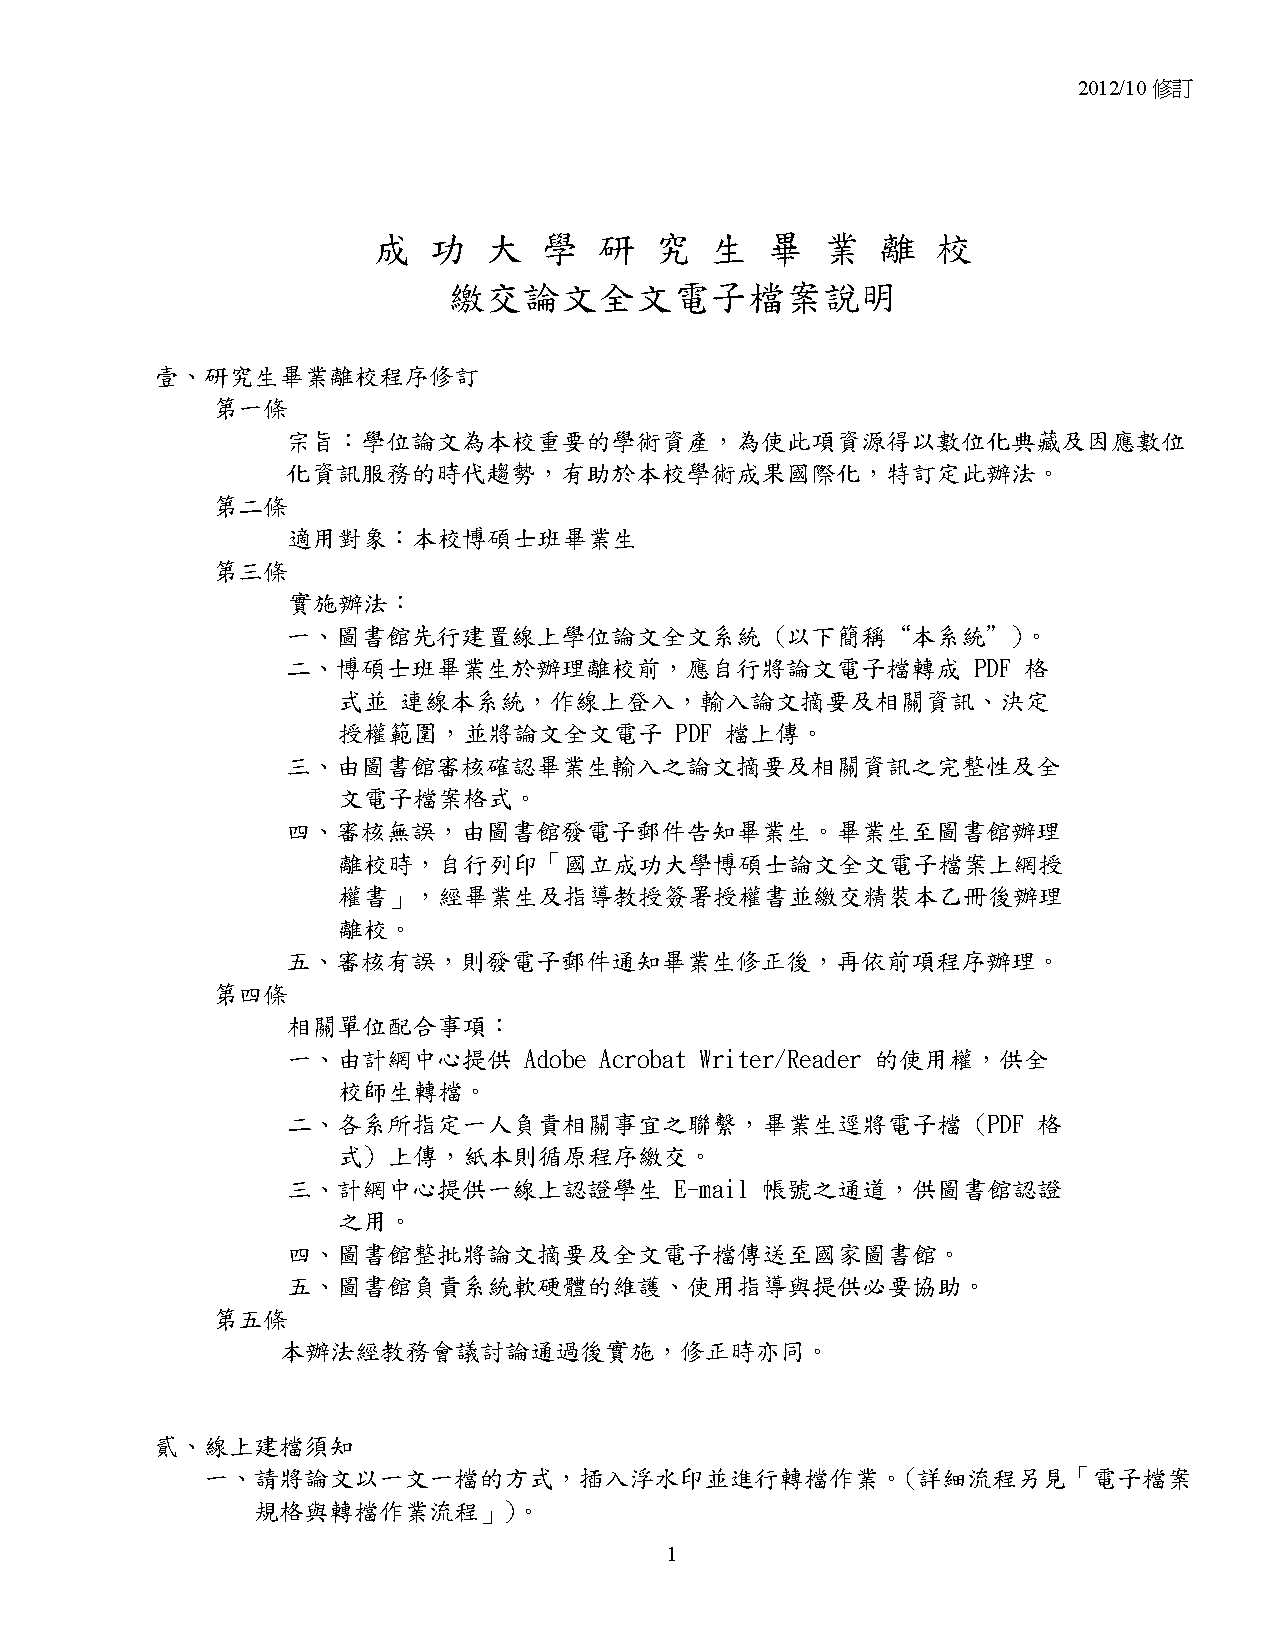
\includepdf[pages=-]{tutorial--pre-PH-fork/appendix/pdf/2012050004-a.pdf}
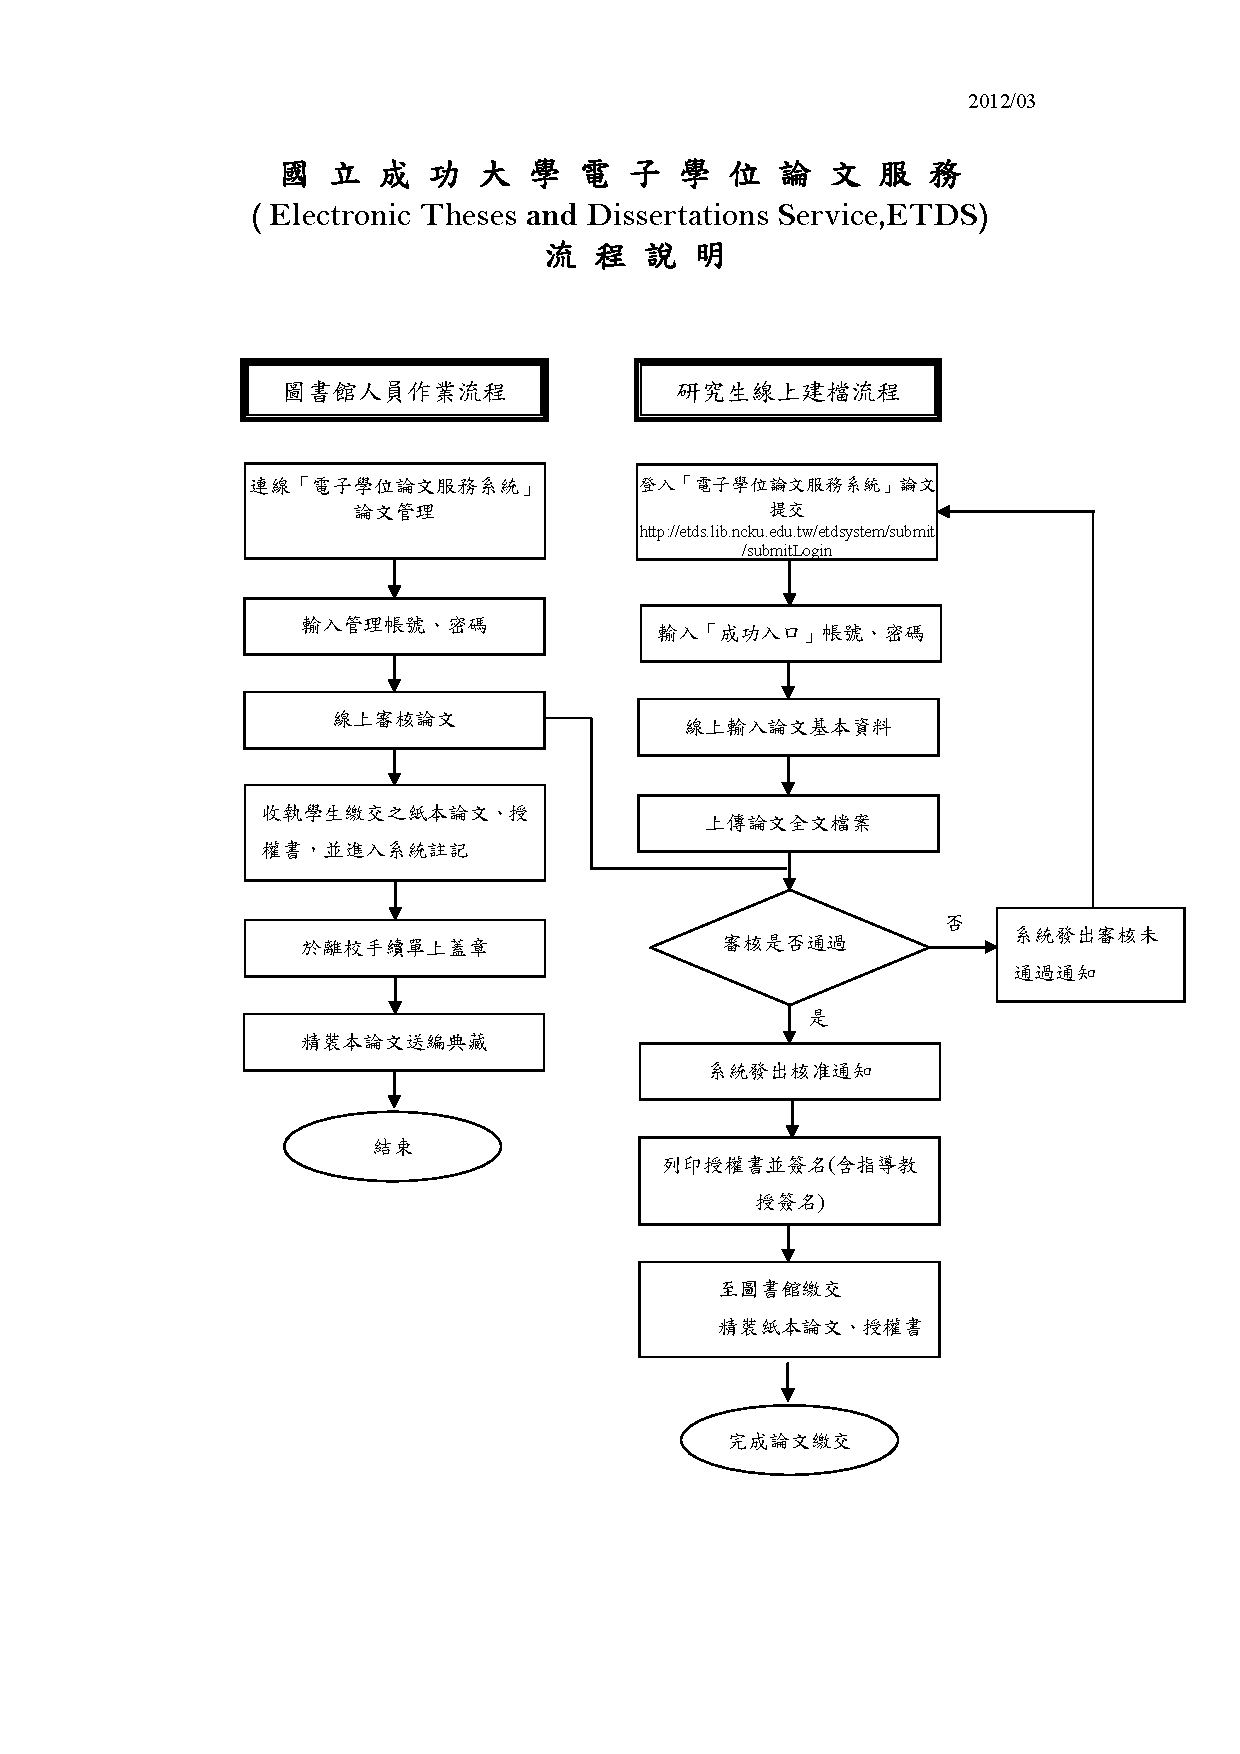
\includepdf[pages=-]{tutorial--pre-PH-fork/appendix/pdf/2012050006-a.pdf}

% ------------------------------------------------
\EndChapter
% ------------------------------------------------

% ------------------------------------------------
\StartChapter{各系所博碩士撰寫論文須知}{appendix:thesis-spec}
% ------------------------------------------------

這部份資料來源是使用'電子學位論文服務'提供'國立成功大學博碩士學位論文格式規範'\RefBib{web:ncku:thesis-need-to-know}.\\

\setboolean{@twoside}{false}
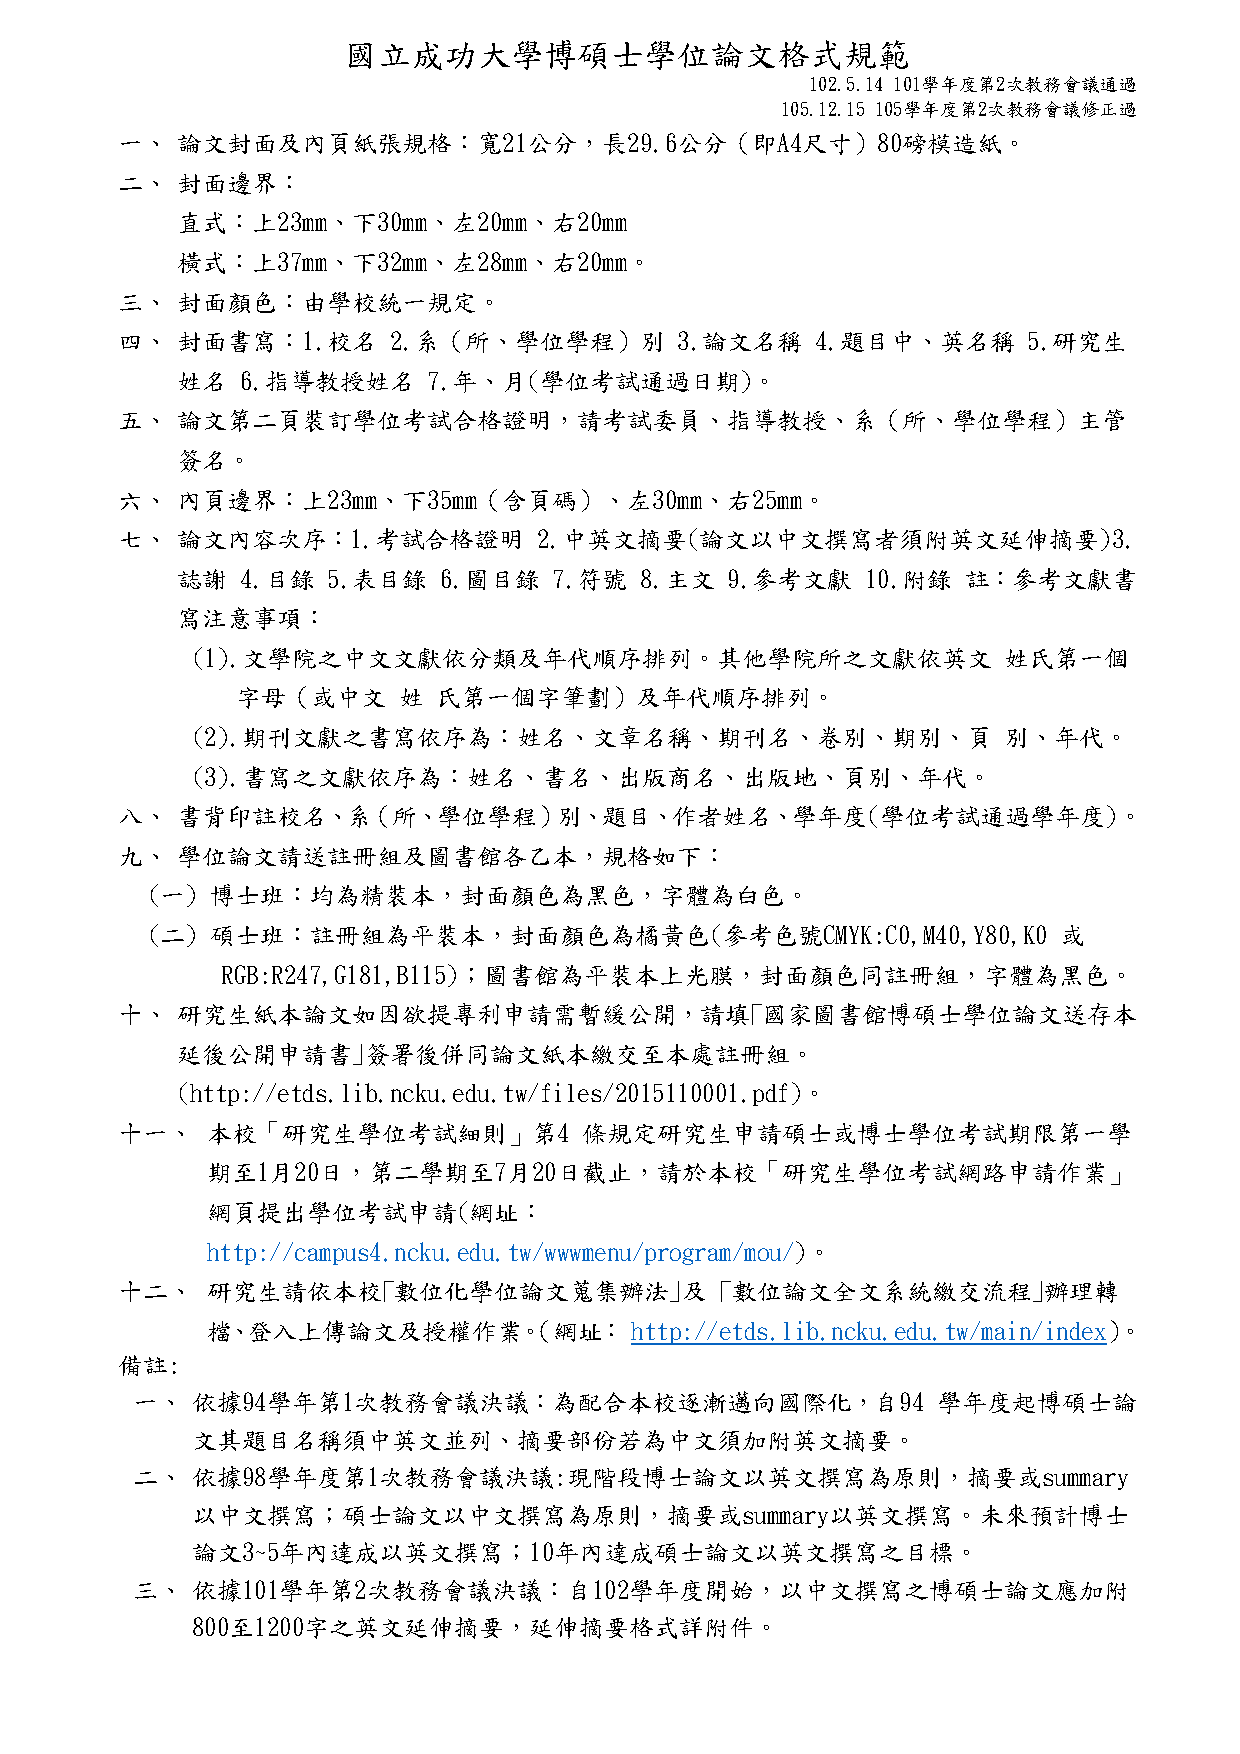
\includepdf[pages=-]{tutorial--pre-PH-fork/appendix/pdf/thesis-spec-a.pdf}

% ------------------------------------------------
\EndChapter
% ------------------------------------------------

% ------------------------------------------------
\StartChapter{電子論文上傳前檢查事項}{appendix:e-paper_upload}
% ------------------------------------------------

這部份資料來源是使用'電子學位論文服務'中的'電子論文上傳前檢查事項'的'2012090001.pdf'\RefBib{web:lib:upload-things-check}.\\

\setboolean{@twoside}{false}
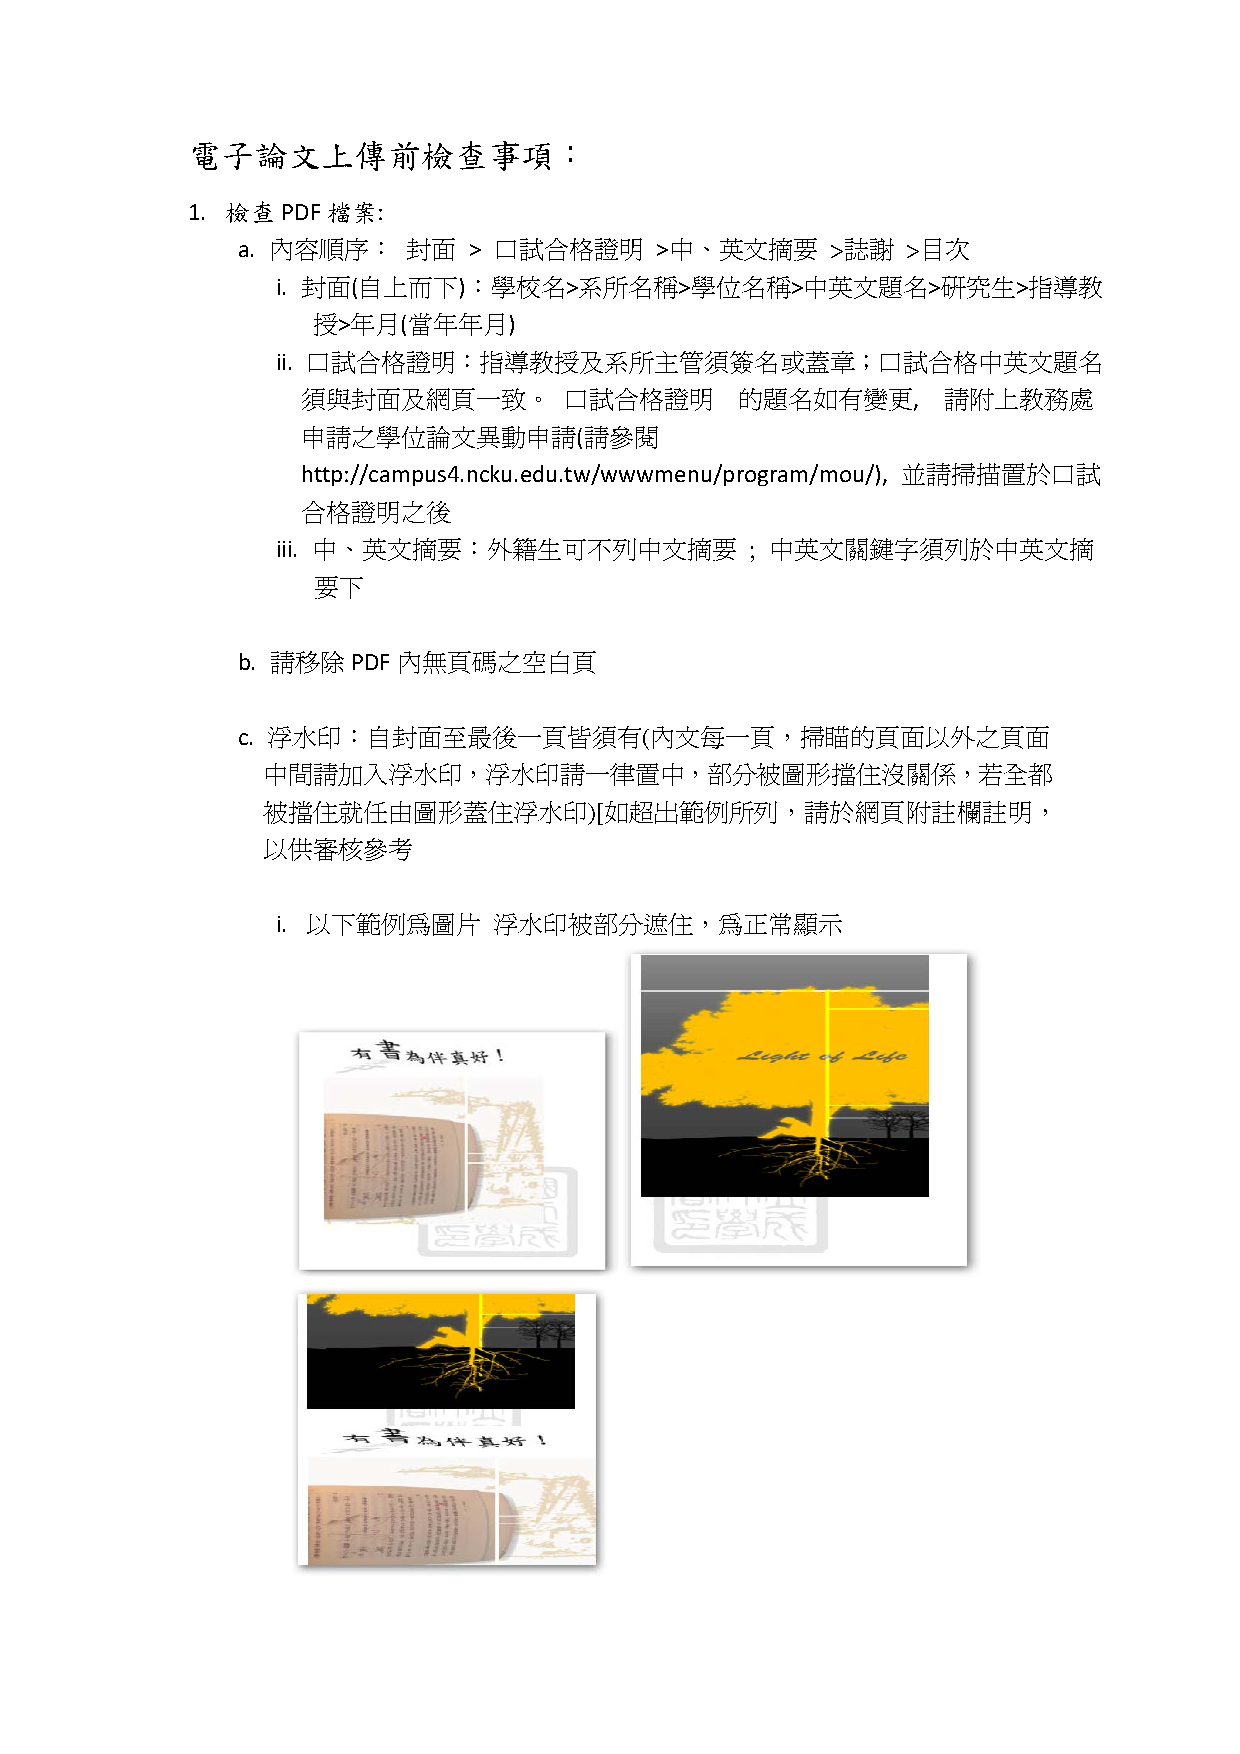
\includepdf[pages=-]{tutorial--pre-PH-fork/appendix/pdf/2012090001-a.pdf}

% ------------------------------------------------
\EndChapter
% ------------------------------------------------

% ------------------------------------------------
\StartChapter{論文提交說明}{appendix:e-paper_upload_ppt}
% ------------------------------------------------

這部份資料來源是使用'電子學位論文服務'提供的 '2016論文提交說明簡報檔'\RefBib{web:lib:2016-submit-ppt} 修改而成的, 只抽出使用本模版後, 還要做什麼的行為.\\

\setboolean{@twoside}{false}
\includepdf[pages=-]{tutorial--pre-PH-fork/appendix/pdf/2012050003-short-a}

% ------------------------------------------------
\EndChapter
% ------------------------------------------------

% ------------------------------------------------
\StartChapter{口試注意事項}
% ------------------------------------------------

這部份資料來源是使用本系資訊工程研究所系辦所提供的資料, 雖然內容主要針對本系, 但某些內容都是適合非本系的同學們.

\setboolean{@twoside}{false}
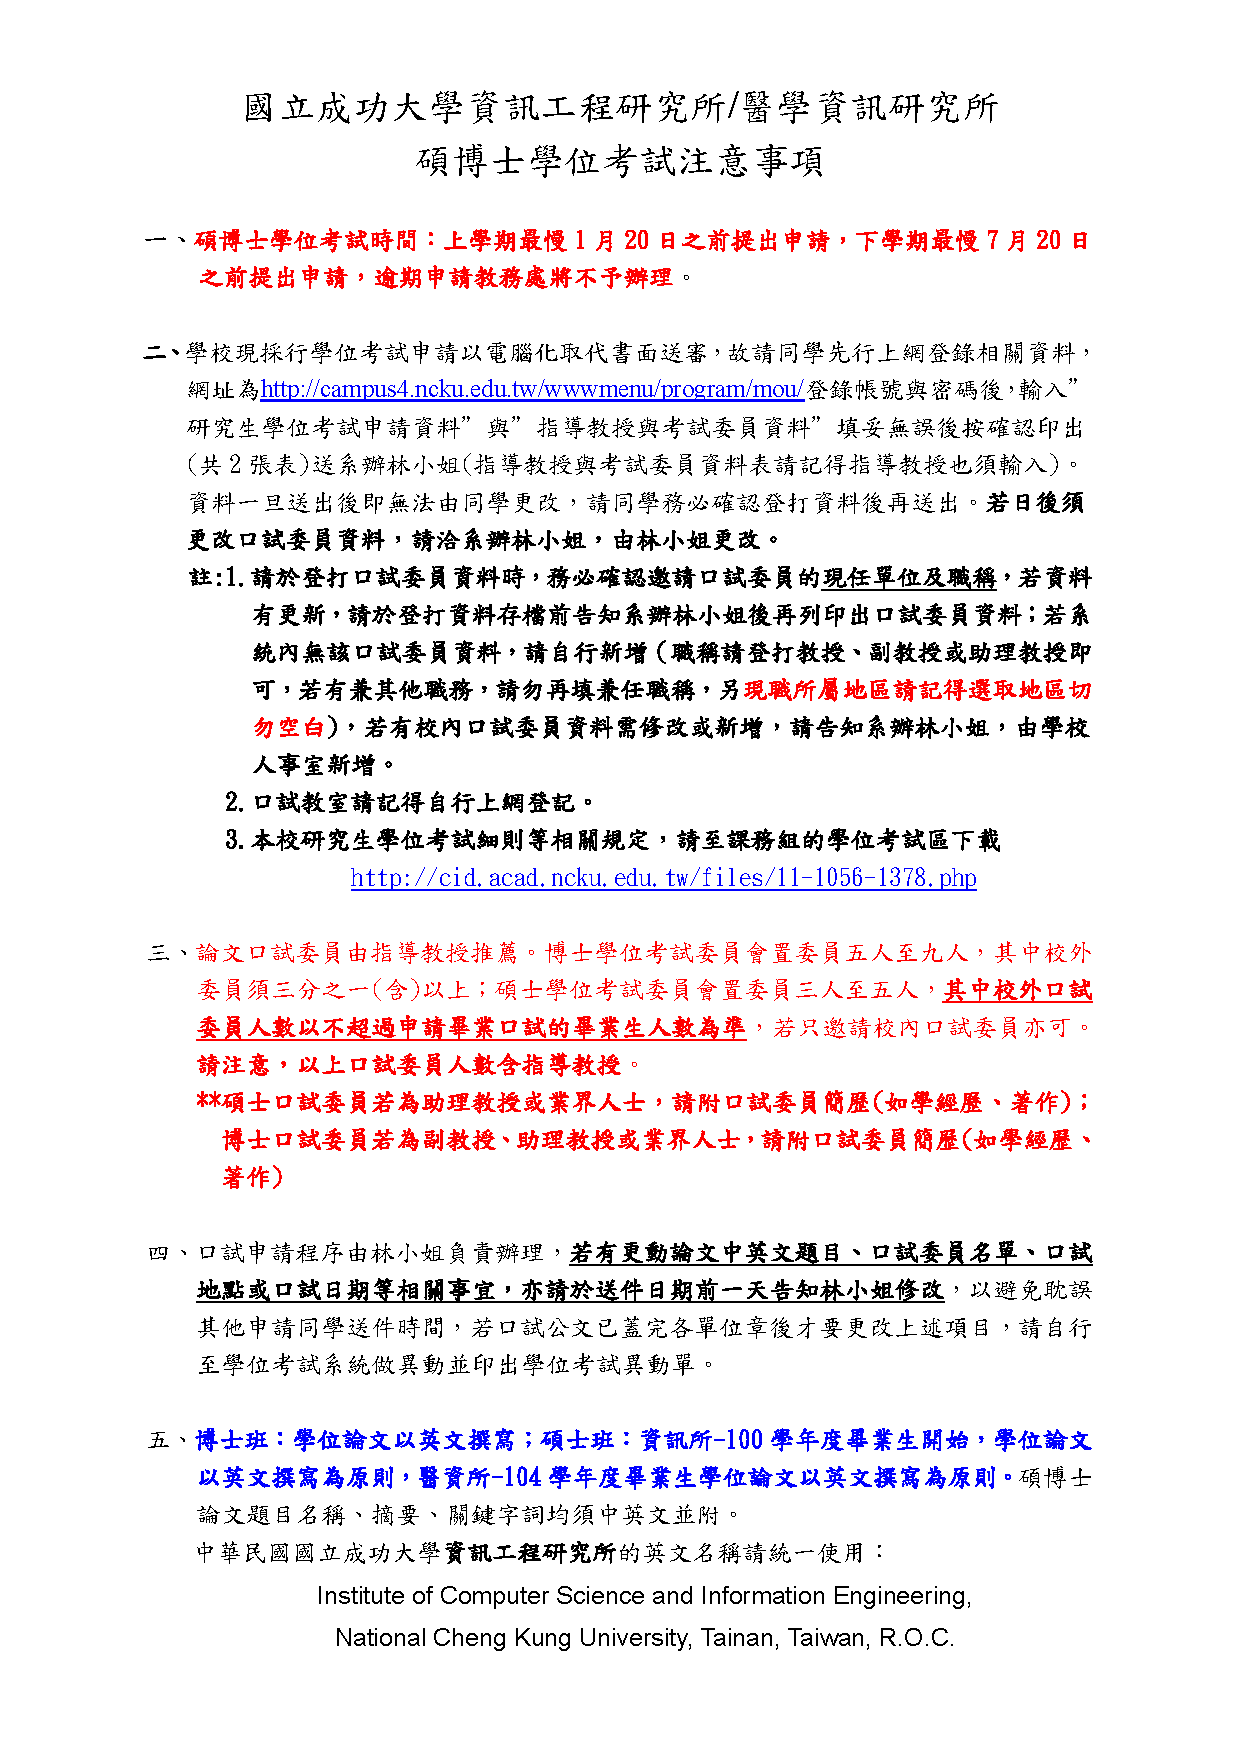
\includepdf[pages=-]{tutorial--pre-PH-fork/appendix/pdf/oral-1040616-a.pdf}

% ------------------------------------------------
\EndChapter
% ------------------------------------------------

% ------------------------------------------------
\StartChapter{常見問題Q\&A}{appendix:faq}
% ------------------------------------------------

這部份資料來源是使用'電子學位論文服務'提供的'FAQ'\RefBib{web:lib:ETDS-QA}, 用來補充其他Appendix沒提到的一些情報.\\

\setboolean{@twoside}{false}
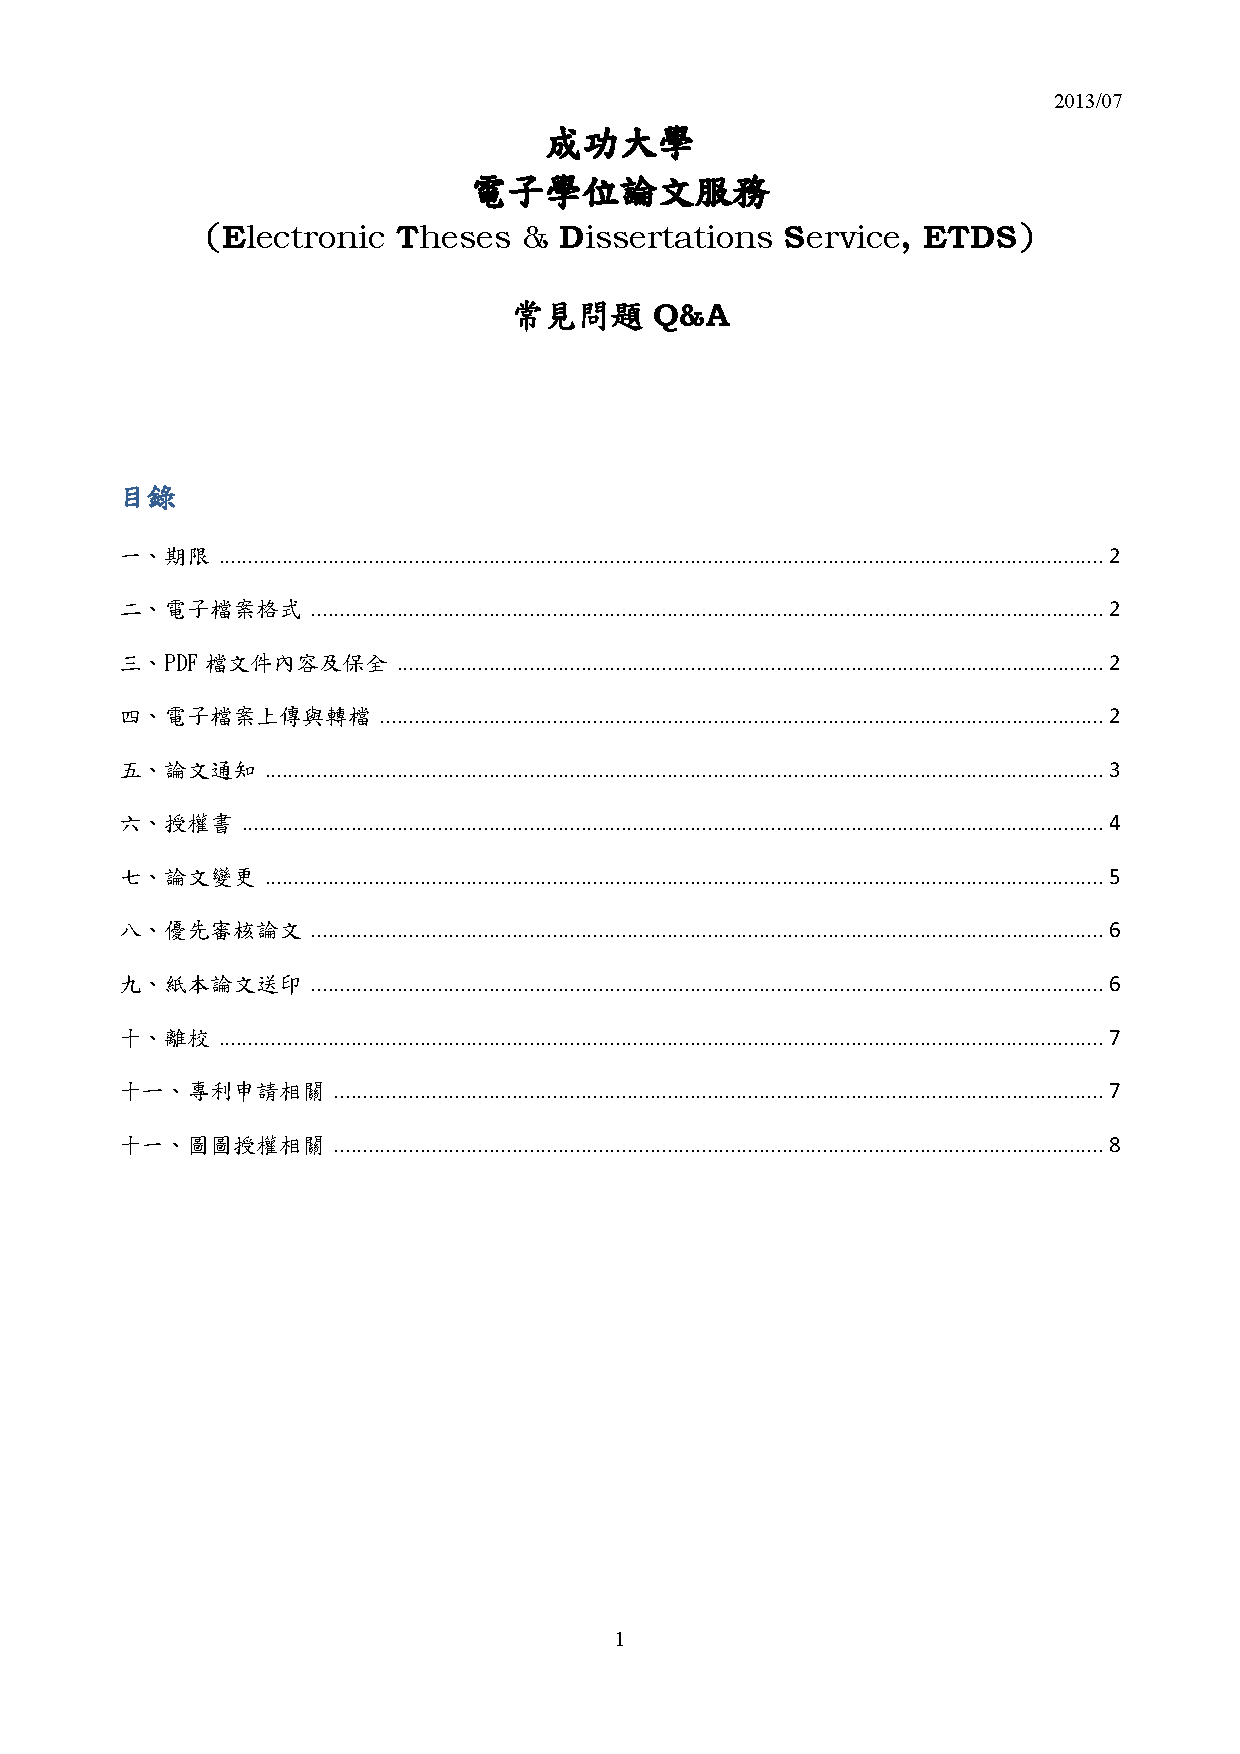
\includepdf[pages=-]{tutorial--pre-PH-fork/appendix/pdf/2012050009-a.pdf}

% ------------------------------------------------
\EndChapter
% ------------------------------------------------

% ------------------------------------------------
\StartChapter{LaTex Symbol寫法}{appendix:unicode-symbols}
% ------------------------------------------------

這部份資料來源是xeCJK的v3.3.4(2016/02/10)版本中提供的50頁有關所有Symbol的寫法, 極度值得同學們閱讀或在這邊找你所需的Symbols.\\

內容的說明方式為:\\
Symbol: 符號所顯示的樣子\\
USV: 以Unicode方式所代表的這個符號, 例如 `(' 的Unicode寫法為U+0028.\\
Description: 是這符號的名字.\\
Macro(s): 是LaTex使用這符號的寫法.\\

\textbf{P.S: }因為符號數量多, 沒法100\%保證全能使用.

\setboolean{@twoside}{false}
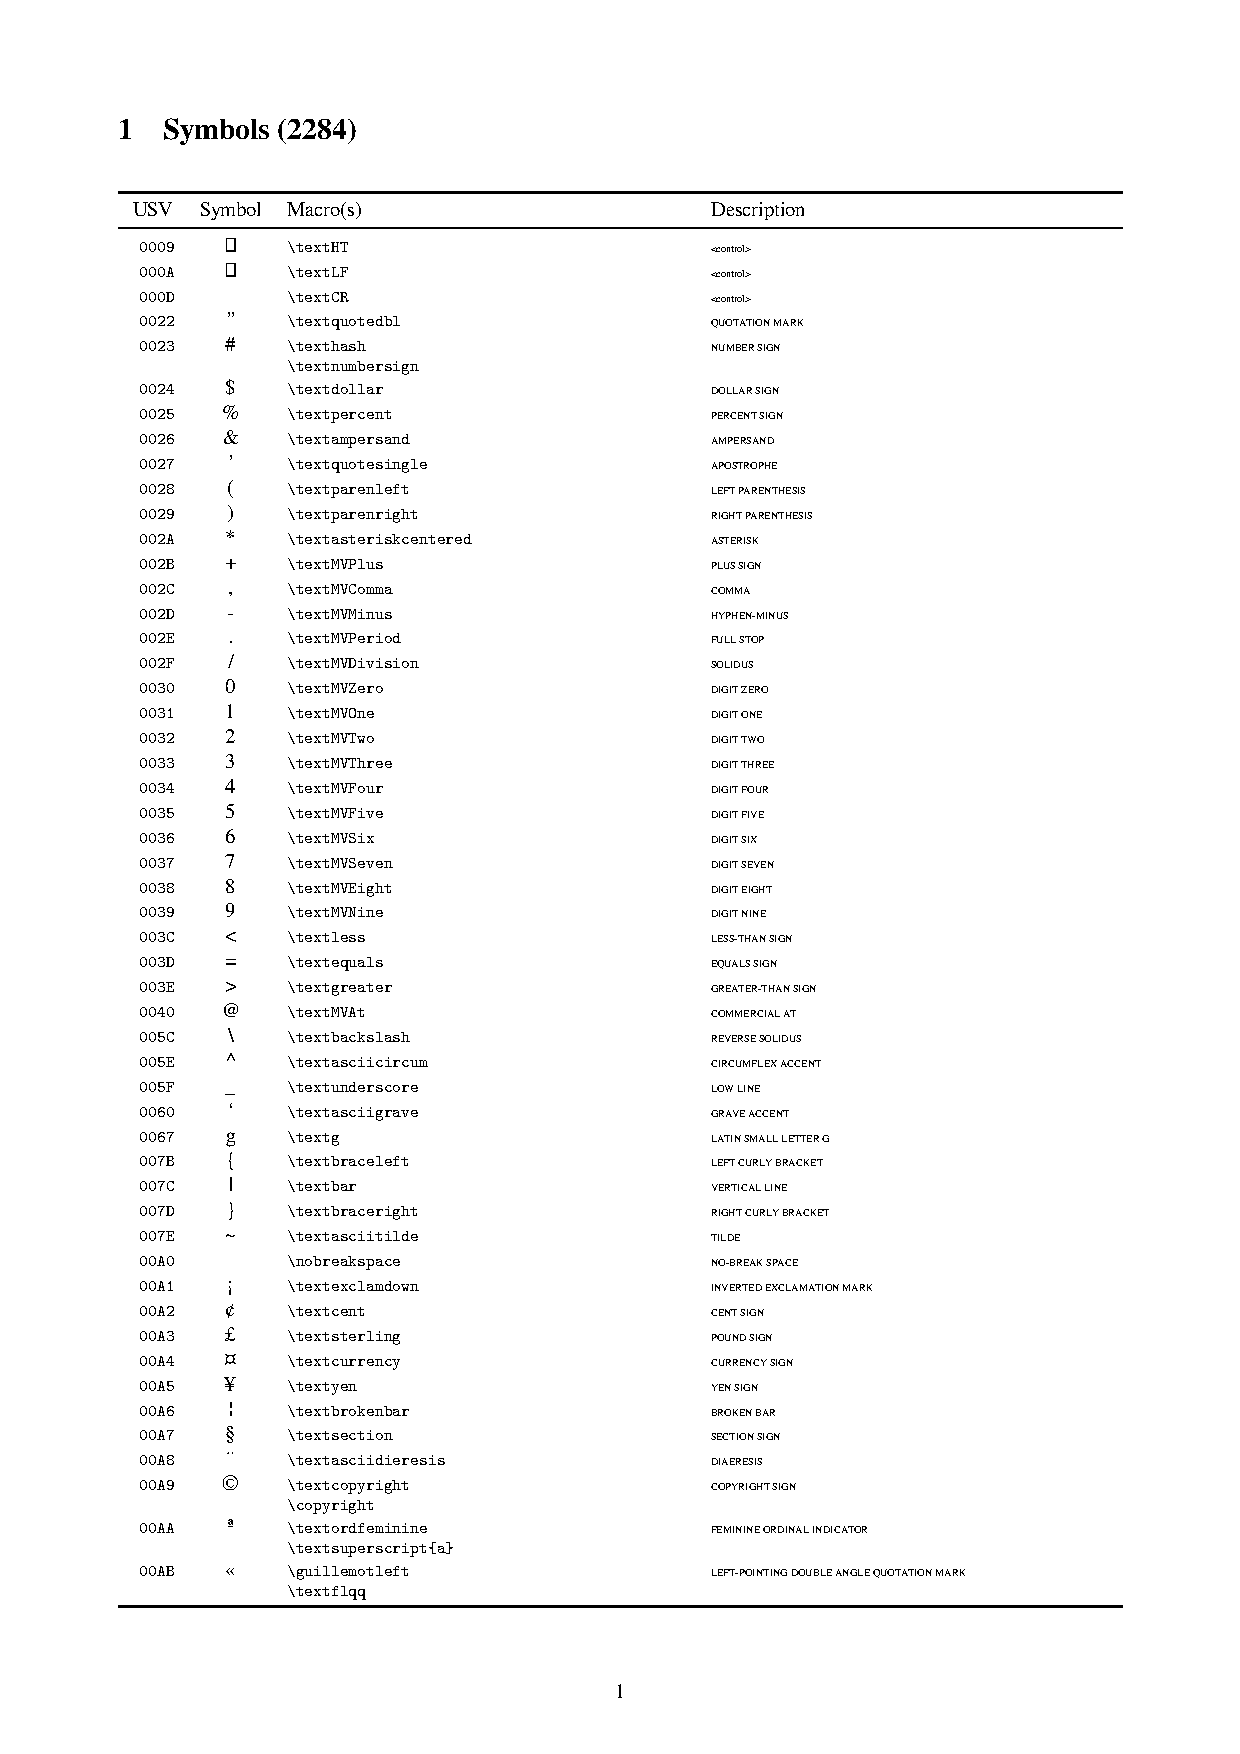
\includepdf[pages=-]{tutorial--pre-PH-fork/appendix/pdf/xunicode-symbols.pdf}

% ------------------------------------------------
\EndChapter
% ------------------------------------------------


% ------------------------------------------------
\EndAppendix
% ------------------------------------------------



% 用來對內容進行不同的設定測試用的測試頁
% ------------------------------------------------
\StartChapter{測試頁 Testing Pages}
% ------------------------------------------------

這邊是用來放置不同的內容來進行測試或設計樣版用的.

% 半形字元與全形字元
% ------------------------------------------------
%
% Reference from:
%
% 半形字元與全形字元
% <https://zh.wikipedia.org/wiki/%E5%85%A8%E5%BD%A2%E5%92%8C%E5%8D%8A%E5%BD%A2>
%
% ------------------------------------------------

\StartSection{半形字元與全形字元的比較 (ASCII字元)}
用來檢查半形/全形字元顯示正常\\

\begin{verbatim}
   全形    半形        |        全形    半形        |        全形    半形
   " "     " "                 !       !                  "       "
    #       #                  $       $                  %       %
    &       &                  '       '                  (       (
    )       )                  *       *                  +       +
    ,       ,                  -       -                  .       .
    /       /

    0       0                 1       1                  2       2
    3       3                 4       4                  5       5
    6       6                 7       7                  8       8
    9       9

    :       :                 ;       ;                  <       <
    =       =                 >       >                  ?       ?
    @       @

    A       A                 B       B                  C       C
    D       D                 E       E                  F       F
    G       G                 H       H                  I       I
    J       J                 K       K                  L       L
    M       M                 N       N                  O       O
    P       P                 Q       Q                  R       R
    S       S                 T       T                  U       U
    V       V                 W       W                  X       X
    Y       Y                 Z       Z

    [       [                 \       \                  ]       ]
    ^       ^                 _       _                  `       `

    a       a                 b       b                  c       c
    d       d                 e       e                  f       f
    g       g                 h       h                  i       i
    j       j                 k       k                  l       l
    m       m                 n       n                  o       o
    p       p                 q       q                  r       r
    s       s                 t       t                  u       u
    v       v                 w       w                  x       x
    y       y                 z       z

    {       {                 |       |                  }       }
    ~       ~
\end{verbatim}

% ------------------------------------------------


% 英文內容
% ------------------------------------------------

\newpage
\StartSection{英文內容 (只用段落來分段)}
用來看內容, 符號, 段距, 字元之間的距離等東西\\

NCKU offers an open learning environment characterized by classical Western and modern eastern landscape. NCKU has attracted numerous distinguished visitors around the world for its rich and welcoming campuses.

In addition to two off-university campuses, An-Nan and Gueiren, the main campus of NCKU consists of 7 satellite campuses adjacent to one another. NCKU occupies a total of more than 180 hectares of land, which tops many other universities in Taiwan. NCKU started out as having only one campus, Cheng Kung, but continued to expand to its current scale. Each campus in the major part of NCKU is closely interlinked and tightly developed as a city within the university.

NCKU's spirit of ``pristine practicality'' and its motto of ``intellectual development through persistent pursuit of knowledge'' have been intrinsic to the thick cultural heritage of the city of Tainan. While members of NCKU are well-integrated with one another, they also work independently. Patrons as NCKU enjoy abundant learning resources.

Through continuous evolution and progression, NCKU has become an active participant in global academia and has earned an excellent reputation in teaching and research. For example, NCKU has ranked the 256th in 2010 Academic Ranking of World Universities announced by Shanghai Jiaotong University and the 80th in 2011 Webometrics Ranking of World Universities published by Centre for Scientific Information and Documentation, Spain, only second to that of NTU, Todai and Kyodai in the Asian region.

% ------------------------------------------------

\newpage
\StartSection{英文內容 (只用強制斷行)}
用來看內容, 符號, 段距, 字元之間的距離等東西\\

NCKU offers an open learning environment characterized by classical Western and modern eastern landscape. NCKU has attracted numerous distinguished visitors around the world for its rich and welcoming campuses.\\
In addition to two off-university campuses, An-Nan and Gueiren, the main campus of NCKU consists of 7 satellite campuses adjacent to one another. NCKU occupies a total of more than 180 hectares of land, which tops many other universities in Taiwan. NCKU started out as having only one campus, Cheng Kung, but continued to expand to its current scale. Each campus in the major part of NCKU is closely interlinked and tightly developed as a city within the university.\\
NCKU's spirit of ``pristine practicality'' and its motto of ``intellectual development through persistent pursuit of knowledge'' have been intrinsic to the thick cultural heritage of the city of Tainan. While members of NCKU are well-integrated with one another, they also work independently. Patrons as NCKU enjoy abundant learning resources.\\
Through continuous evolution and progression, NCKU has become an active participant in global academia and has earned an excellent reputation in teaching and research. For example, NCKU has ranked the 256th in 2010 Academic Ranking of World Universities announced by Shanghai Jiaotong University and the 80th in 2011 Webometrics Ranking of World Universities published by Centre for Scientific Information and Documentation, Spain, only second to that of NTU, Todai and Kyodai in the Asian region.

% ------------------------------------------------

\newpage
\StartSection{英文內容 (段落 + 強制斷行)}
用來看內容, 符號, 段距, 字元之間的距離等東西\\

NCKU offers an open learning environment characterized by classical Western and modern eastern landscape. NCKU has attracted numerous distinguished visitors around the world for its rich and welcoming campuses.\\

In addition to two off-university campuses, An-Nan and Gueiren, the main campus of NCKU consists of 7 satellite campuses adjacent to one another. NCKU occupies a total of more than 180 hectares of land, which tops many other universities in Taiwan. NCKU started out as having only one campus, Cheng Kung, but continued to expand to its current scale. Each campus in the major part of NCKU is closely interlinked and tightly developed as a city within the university.\\

NCKU's spirit of ``pristine practicality'' and its motto of ``intellectual development through persistent pursuit of knowledge'' have been intrinsic to the thick cultural heritage of the city of Tainan. While members of NCKU are well-integrated with one another, they also work independently. Patrons as NCKU enjoy abundant learning resources.\\

Through continuous evolution and progression, NCKU has become an active participant in global academia and has earned an excellent reputation in teaching and research. For example, NCKU has ranked the 256th in 2010 Academic Ranking of World Universities announced by Shanghai Jiaotong University and the 80th in 2011 Webometrics Ranking of World Universities published by Centre for Scientific Information and Documentation, Spain, only second to that of NTU, Todai and Kyodai in the Asian region.

% ------------------------------------------------


% 中文內容
% ------------------------------------------------

\newpage
\StartSection{中文內容 (只用段落來分段)}
用來看內容, 符號, 段距, 字元之間的距離等東西\\

本校創校於西元1931年(昭和6年,民國20年)1月15日,原名為「臺南高等工業學校」;1944年(昭和19年,民國33年)改稱為「臺南工業專門學校」。民國34年臺灣光復。本校於民國35年2月改制為「臺灣省立臺南工業專科學校」,由王石安博士擔任校長;35年10月改制為「臺灣省立工學院」,仍由王石安博士擔任校長。彼時僅有成功校區,39年增購勝利校區。41年2月,由秦大鈞博士接任校長。

45年8月,本校改制為「臺灣省立成功大學」,仍由秦大鈞博士擔任校長;同時增設文理學院及商學院。46年8月,由閻振興博士接任校長。54年1月,由羅雲平博士接任校長。55年增購光復校區。58年10月,將文理學院分為文學院及理學院。60年8月,改制為「國立成功大學」,並由倪超博士接任校長;同年增購建國校區。67年8月,由王唯農博士接任校長。

69年8月,夏漢民博士接任校長;同年將商學院更名為管理學院。72年8月,增設醫學院,並增購自強校區及敬業校區。74年增購力行校區部分校地。76年增購歸仁校區,設置航空太空實驗場。77年6月本校醫學院附設醫院正式營運。77年8月,馬哲儒博士接任校長。80年增購自強校區北半部。82年陸續增購台南市「文大五」用地,闢為本校安南校區。

83年8月,吳京院士接任校長。吳校長於85年6月入閣擔任教育部長,由副校長黃定加博士代理校長。86年2月,翁政義博士接任校長。86年8月增設社會科學院。88年完成收購安南校區全部校地;同年6月增購原陸軍八○四醫院用地(91年6月完成撥用手續)。翁校長於89年5月出任國科會主委,由副校長翁鴻山博士代理校長。90年2月,高強博士接任校長。92年8月,增設電機資訊學院、規劃與設計學院。94年7月,本校配合國軍斗六醫院精實案,接管該院營運權,設置為雲林縣斗六校區,並改制為本校醫學院附設醫院斗六分院。94年8月,增設生物科學與科技學院。94年10月,本校得到教育部的肯定,獲選為「發展國際一流大學及頂尖研究中心計畫」的兩所重點大學之一。

96年2月,賴明詔院士接任校長,97年2月教育部公佈「發展國際一流大學及頂尖研究中心計畫」第二梯次的審議結果,本校繼續獲得教育部的肯定與補助,積極朝國際一流大學的目標邁進。97年10月增購歸仁校區北側台糖土地(正式登記為本校管有)。100年2月,黃煌煇博士接任校長。100年4月本校獲得教育部第二期頂尖大學計畫補助,持續朝國際一流大學的目標邁進。104年2月,蘇慧貞博士接任校長。

% ------------------------------------------------

\newpage
\StartSection{中文內容 (只用強制斷行)}
用來看內容, 符號, 段距, 字元之間的距離等東西\\

本校創校於西元1931年(昭和6年,民國20年)1月15日,原名為「臺南高等工業學校」;1944年(昭和19年,民國33年)改稱為「臺南工業專門學校」。民國34年臺灣光復。本校於民國35年2月改制為「臺灣省立臺南工業專科學校」,由王石安博士擔任校長;35年10月改制為「臺灣省立工學院」,仍由王石安博士擔任校長。彼時僅有成功校區,39年增購勝利校區。41年2月,由秦大鈞博士接任校長。\\
45年8月,本校改制為「臺灣省立成功大學」,仍由秦大鈞博士擔任校長;同時增設文理學院及商學院。46年8月,由閻振興博士接任校長。54年1月,由羅雲平博士接任校長。55年增購光復校區。58年10月,將文理學院分為文學院及理學院。60年8月,改制為「國立成功大學」,並由倪超博士接任校長;同年增購建國校區。67年8月,由王唯農博士接任校長。\\
69年8月,夏漢民博士接任校長;同年將商學院更名為管理學院。72年8月,增設醫學院,並增購自強校區及敬業校區。74年增購力行校區部分校地。76年增購歸仁校區,設置航空太空實驗場。77年6月本校醫學院附設醫院正式營運。77年8月,馬哲儒博士接任校長。80年增購自強校區北半部。82年陸續增購台南市「文大五」用地,闢為本校安南校區。\\
83年8月,吳京院士接任校長。吳校長於85年6月入閣擔任教育部長,由副校長黃定加博士代理校長。86年2月,翁政義博士接任校長。86年8月增設社會科學院。88年完成收購安南校區全部校地;同年6月增購原陸軍八○四醫院用地(91年6月完成撥用手續)。翁校長於89年5月出任國科會主委,由副校長翁鴻山博士代理校長。90年2月,高強博士接任校長。92年8月,增設電機資訊學院、規劃與設計學院。94年7月,本校配合國軍斗六醫院精實案,接管該院營運權,設置為雲林縣斗六校區,並改制為本校醫學院附設醫院斗六分院。94年8月,增設生物科學與科技學院。94年10月,本校得到教育部的肯定,獲選為「發展國際一流大學及頂尖研究中心計畫」的兩所重點大學之一。\\
96年2月,賴明詔院士接任校長,97年2月教育部公佈「發展國際一流大學及頂尖研究中心計畫」第二梯次的審議結果,本校繼續獲得教育部的肯定與補助,積極朝國際一流大學的目標邁進。97年10月增購歸仁校區北側台糖土地(正式登記為本校管有)。100年2月,黃煌煇博士接任校長。100年4月本校獲得教育部第二期頂尖大學計畫補助,持續朝國際一流大學的目標邁進。104年2月,蘇慧貞博士接任校長。

% ------------------------------------------------

\newpage
\StartSection{中文內容 (段落 + 強制斷行)}
用來看內容, 符號, 段距, 字元之間的距離等東西\\

本校創校於西元1931年(昭和6年,民國20年)1月15日,原名為「臺南高等工業學校」;1944年(昭和19年,民國33年)改稱為「臺南工業專門學校」。民國34年臺灣光復。本校於民國35年2月改制為「臺灣省立臺南工業專科學校」,由王石安博士擔任校長;35年10月改制為「臺灣省立工學院」,仍由王石安博士擔任校長。彼時僅有成功校區,39年增購勝利校區。41年2月,由秦大鈞博士接任校長。\\

45年8月,本校改制為「臺灣省立成功大學」,仍由秦大鈞博士擔任校長;同時增設文理學院及商學院。46年8月,由閻振興博士接任校長。54年1月,由羅雲平博士接任校長。55年增購光復校區。58年10月,將文理學院分為文學院及理學院。60年8月,改制為「國立成功大學」,並由倪超博士接任校長;同年增購建國校區。67年8月,由王唯農博士接任校長。\\

69年8月,夏漢民博士接任校長;同年將商學院更名為管理學院。72年8月,增設醫學院,並增購自強校區及敬業校區。74年增購力行校區部分校地。76年增購歸仁校區,設置航空太空實驗場。77年6月本校醫學院附設醫院正式營運。77年8月,馬哲儒博士接任校長。80年增購自強校區北半部。82年陸續增購台南市「文大五」用地,闢為本校安南校區。\\

83年8月,吳京院士接任校長。吳校長於85年6月入閣擔任教育部長,由副校長黃定加博士代理校長。86年2月,翁政義博士接任校長。86年8月增設社會科學院。88年完成收購安南校區全部校地;同年6月增購原陸軍八○四醫院用地(91年6月完成撥用手續)。翁校長於89年5月出任國科會主委,由副校長翁鴻山博士代理校長。90年2月,高強博士接任校長。92年8月,增設電機資訊學院、規劃與設計學院。94年7月,本校配合國軍斗六醫院精實案,接管該院營運權,設置為雲林縣斗六校區,並改制為本校醫學院附設醫院斗六分院。94年8月,增設生物科學與科技學院。94年10月,本校得到教育部的肯定,獲選為「發展國際一流大學及頂尖研究中心計畫」的兩所重點大學之一。\\

96年2月,賴明詔院士接任校長,97年2月教育部公佈「發展國際一流大學及頂尖研究中心計畫」第二梯次的審議結果,本校繼續獲得教育部的肯定與補助,積極朝國際一流大學的目標邁進。97年10月增購歸仁校區北側台糖土地(正式登記為本校管有)。100年2月,黃煌煇博士接任校長。100年4月本校獲得教育部第二期頂尖大學計畫補助,持續朝國際一流大學的目標邁進。104年2月,蘇慧貞博士接任校長。

% ------------------------------------------------


% 混合的中英文內容
% ------------------------------------------------

\newpage
\StartSection{混合的中英文內容 (只用段落來分段)}
用來看內容, 符號, 段距, 字元之間的距離等東西\\

Google公司(英語:Google Inc.; 中文:穀歌[3]、穀歌[4]、科高[5]), 是一家美國的跨國科技企業, 業務範圍涵蓋互聯網搜索、雲計算、廣告技術等領域, 開發並提供大量基於互聯網的產品與服務[6], 其主要利潤來自於AdWords等廣告服務[7][8].

\begin{description}
\item [Google] Google由在斯坦福大學攻讀理工博士的拉裡•佩奇和謝爾蓋•布林共同創建, 因此兩人也被稱為``Google Guys''[9][10][11]. 1998年9月4日, Google以私營公司的形式創立, 目的是設計並管理互聯網搜尋引擎``Google搜索''. 2004年8月19日, Google公司在納斯達克上市, 後來被稱為``三駕馬車''的公司兩位共同創始人與出任首席執行官的埃裡克•施密特在此時承諾:共同在Google工作至少二十年, 即至2024年止[12].

\item [Google]\hfill\\ Google由在斯坦福大學攻讀理工博士的拉裡•佩奇和謝爾蓋•布林共同創建, 因此兩人也被稱為``Google Guys''[9][10][11]. 1998年9月4日, Google以私營公司的形式創立, 目的是設計並管理互聯網搜尋引擎``Google搜索''. 2004年8月19日, Google公司在納斯達克上市, 後來被稱為``三駕馬車''的公司兩位共同創始人與出任首席執行官的埃裡克•施密特在此時承諾:共同在Google工作至少二十年, 即至2024年止[12].

\item Google的宗旨是``整合全球範圍的資訊, 使人人皆可訪問並從中受益''(To organize the world's information and make it universally accessible and useful)[13]; 而非正式的口號則為``不作惡''(Don't be evil), 由工程師阿米特•派特爾(Amit Patel)所創[14], 並得到了保羅•布赫海特的支持[15][16]. Google公司的總部稱為``Googleplex'', 位於美國加州聖克拉拉縣的山景城. 2011年4月, 佩奇接替施密特擔任首席執行官[17].

\item 在2015年8月, Google進行宣佈資產重組. 重組後, Google劃歸新成立的Alphabet底下. 同時, 此舉把Google旗下的核心搜索和廣告業務與Google無人車等新興業務分離開來[18].
\end{description}

據估計, Google在全世界的資料中心內運營著上百萬台的伺服器, [19]每天處理數以億計的搜索請求[20]和約二十四PB使用者生成的資料. [21][22][23][24] Google自創立起開始的快速成長同時也帶動了一系列的產品研發、並購事項與合作關係, 而不僅僅是公司核心的網路搜索業務. Google公司提供豐富的線上軟體服務, 如雲端硬碟、Gmail電子郵件, 包括Orkut、Google Buzz以及Google+在內的社交網路服務. Google的產品同時也以應用軟體的形式進入使用者桌面, 例如Google Chrome網頁流覽器、Picasa圖片整理與編輯軟體、Google Talk即時通訊工具等. 另外, Google還進行了移動設備的Android作業系統以及Google Chrome OS作業系統的開發. [25]

資訊分析網站Alexa資料顯示, Google的主功能變數名稱google.com是全世界訪問量最高的網站, Google搜索在其他國家或地區域名下的多個網站(google.co.in、google.de、google.com.hk等等), 及旗下的YouTube、Blogger、Orkut等的訪問量都在前一百名之內. [26]其中, 社交網路服務Orkut於2014年9月關閉. [27]

Facebook(原本稱作thefacebook)是一家位於美國加州聖馬刁郡門洛派克市的線上社交網路服務網站. 其名稱的靈感來自美國高中提供給學生包含照片和聯絡資料的通訊錄(或稱花名冊)暱稱「face book」[6][7].

除了文字訊息之外, 使用者可傳送圖片、影片和聲音媒體訊息(現在也可以傳送其他檔案類型如.doc,.docx,.xls,.xlsx等, 但是.exe可能會被禁止傳送)給其他使用者, 以及透過整合的地圖功能分享使用者的所在位置. Facebook是在2004年2月4日由馬克•紮克伯格與他的哈佛大學室友們所創立[8]. Facebook的會員最初只限於哈佛學生加入, 但後來逐漸擴展到其他在波士頓區域的同學也能使用, 包括一些常春藤名校、MIT、紐約大學、史丹福大學等. 接著逐漸支援讓其他大學和高中學生加入, 並在最後開放給任何13歲或以上的人使用.  現在Facebook允許任何聲明自己年滿13歲的使用者註冊[9].

使用者必須註冊才能使用Facebook, 註冊後他們可以創建個人檔案、將其他使用者加為好友、傳遞訊息, 並在其他使用者更新個人檔案時獲得自動通知. 此外使用者也可以加入有相同興趣的群組, 這些群組依據工作地點、學校或其他特性分類. 使用者亦可將朋友分別加入不同的列表中管理, 例如「同事」或「摯友」等. 截至2012年9月, Facebook內已有超過十幾億個活躍使用者[10], 其中約有9\%的不實使用者[11]. 截至2012年, Facebook每年共產生180拍位元組(PB)的資料, 並以每24小時0.5拍位元元組的速度增加[12]. 統計顯示, Facebook上每天上傳3億5千萬張圖片. [13]

Facebook創始人馬克•紮克伯格是世界上最著名的CEO之一. 而馬克•紮克伯格曾經的朋友與商業合作夥伴愛德華多•薩維林在新加坡亦十分知名[14].

Google公司(英語:Google Inc.; 中文:穀歌[3]、穀歌[4]、科高[5]), 是一家美國的跨國科技企業, 業務範圍涵蓋互聯網搜索、雲計算、廣告技術等領域, 開發並提供大量基於互聯網的產品與服務[6], 其主要利潤來自於AdWords等廣告服務[7][8].

\begin{itemize}
\item Google由在斯坦福大學攻讀理工博士的拉裡•佩奇和謝爾蓋•布林共同創建, 因此兩人也被稱為``Google Guys''[9][10][11]. 1998年9月4日, Google以私營公司的形式創立, 目的是設計並管理互聯網搜尋引擎``Google搜索''. 2004年8月19日, Google公司在納斯達克上市, 後來被稱為``三駕馬車''的公司兩位共同創始人與出任首席執行官的埃裡克•施密特在此時承諾:共同在Google工作至少二十年, 即至2024年止[12].

\item Google的宗旨是``整合全球範圍的資訊, 使人人皆可訪問並從中受益''(To organize the world's information and make it universally accessible and useful)[13];
\begin{itemize}
\item Google的宗旨是``整合全球範圍的資訊, 使人人皆可訪問並從中受益''(To organize the world's information and make it universally accessible and useful)[13]; 而非正式的口號則為``不作惡''(Don't be evil), 由工程師阿米特•派特爾(Amit Patel)所創[14], 並得到了保羅•布赫海特的支持[15][16]. Google公司的總部稱為``Googleplex'', 位於美國加州聖克拉拉縣的山景城. 2011年4月, 佩奇接替施密特擔任首席執行官[17].
\item Google的宗旨是``整合全球範圍的資訊, 使人人皆可訪問並從中受益''(To organize the world's information and make it universally accessible and useful)[13].
\item Google公司的總部稱為``Googleplex'', 位於美國加州聖克拉拉縣的山景城. 2011年4月, 佩奇接替施密特擔任首席執行官[17].
\end{itemize}

\item 在2015年8月, Google進行宣佈資產重組. 重組後, Google劃歸新成立的Alphabet底下. 同時, 此舉把Google旗下的核心搜索和廣告業務與Google無人車等新興業務分離開來[18].
\end{itemize}

據估計, Google在全世界的資料中心內運營著上百萬台的伺服器, [19]每天處理數以億計的搜索請求[20]和約二十四PB使用者生成的資料. [21][22][23][24] Google自創立起開始的快速成長同時也帶動了一系列的產品研發、並購事項與合作關係, 而不僅僅是公司核心的網路搜索業務. Google公司提供豐富的線上軟體服務, 如雲端硬碟、Gmail電子郵件, 包括Orkut、Google Buzz以及Google+在內的社交網路服務. Google的產品同時也以應用軟體的形式進入使用者桌面, 例如Google Chrome網頁流覽器、Picasa圖片整理與編輯軟體、Google Talk即時通訊工具等. 另外, Google還進行了移動設備的Android作業系統以及Google Chrome OS作業系統的開發. [25]

資訊分析網站Alexa資料顯示, Google的主功能變數名稱google.com是全世界訪問量最高的網站, Google搜索在其他國家或地區域名下的多個網站(google.co.in、google.de、google.com.hk等等), 及旗下的YouTube、Blogger、Orkut等的訪問量都在前一百名之內. [26]其中, 社交網路服務Orkut於2014年9月關閉. [27]

Facebook(原本稱作thefacebook)是一家位於美國加州聖馬刁郡門洛派克市的線上社交網路服務網站. 其名稱的靈感來自美國高中提供給學生包含照片和聯絡資料的通訊錄(或稱花名冊)暱稱「face book」[6][7].
\begin{enumerate}
\item 除了文字訊息之外, 使用者可傳送圖片、影片和聲音媒體訊息(現在也可以傳送其他檔案類型如.doc,.docx,.xls,.xlsx等, 但是.exe可能會被禁止傳送)給其他使用者, 以及透過整合的地圖功能分享使用者的所在位置.

\item Facebook是在2004年2月4日由馬克•紮克伯格與他的哈佛大學室友們所創立[8]. Facebook的會員最初只限於哈佛學生加入, 但後來逐漸擴展到其他在波士頓區域的同學也能使用, 包括一些常春藤名校、MIT、紐約大學、史丹福大學等.

\item 接著逐漸支援讓其他大學和高中學生加入, 並在最後開放給任何13歲或以上的人使用.  現在Facebook允許任何聲明自己年滿13歲的使用者註冊[9].
\end{enumerate}
使用者必須註冊才能使用Facebook, 註冊後他們可以創建個人檔案、將其他使用者加為好友、傳遞訊息, 並在其他使用者更新個人檔案時獲得自動通知. 此外使用者也可以加入有相同興趣的群組, 這些群組依據工作地點、學校或其他特性分類. 使用者亦可將朋友分別加入不同的列表中管理, 例如「同事」或「摯友」等. 截至2012年9月, Facebook內已有超過十幾億個活躍使用者[10], 其中約有9\%的不實使用者[11]. 截至2012年, Facebook每年共產生180拍位元組(PB)的資料, 並以每24小時0.5拍位元元組的速度增加[12]. 統計顯示, Facebook上每天上傳3億5千萬張圖片. [13]

Facebook創始人馬克•紮克伯格是世界上最著名的CEO之一. 而馬克•紮克伯格曾經的朋友與商業合作夥伴愛德華多•薩維林在新加坡亦十分知名[14].

% ------------------------------------------------


% 表格
% ------------------------------------------------

\newpage
\StartSection{Table使用透明度}

\vspace{3.0cm}

\InsertTable
  [caption={opacity使用預設}]
  {
    \begin{tabular}{llll}
    \hline
    Engine &  &  & OPEL Astra C16SE \\ \hline
    Displacement (cc) &  &  & 1598 \\
    Bore x stroke(mm x mm) &  &  & 79 x 81.5 \\
    Value mechanism &  &  & SOHC \\
    Number of valves &  &  & Intake 4, exhaust 4 \\
    Compression ratio &  &  & 9.8:1 \\
    Torque &  &  & 135/3400 Nm/rpm \\
    Power &  &  & 74/5800 kW/rpm \\
    Ignition sequence &  &  & 1-3-4-2 \\
    Spark plug &  &  & BPR6ES \\
    Fuel &  &  & 95 unleaded gasoline \\
    Cylinder arrangment &  &  & In-line 4 cylinders \\ \hline
    \end{tabular}
  } % End of  \InsertTable{}

  \InsertTable
    [caption={測試opacity=0.4},
      opacity=0.4]
    {
      \begin{tabular}{|c|c|c|c|c|c|c|c|c|c|c|c|c|c|c|c|}
      \hline
       & Col 1 & Col 2 & Col 3 & Col 4 & Col 5 & Col 6 & Col 7 & Col 8 & Col 9 & Col 10 & Col 11 & Col 12 & Col 13 & Col 14 \\ \hline
      Row 1 & Value & Value & Value & Value & Value & Value & Value & Value & Value & Value & Value & Value & Value & Value \\ \hline
      Row 2 & Value & Value & Value & Value & Value & Value & Value & Value & Value & Value & Value & Value & Value & Value \\ \hline
      Row 3 & Value & Value & Value & Value & Value & Value & Value & Value & Value & Value & Value & Value & Value & Value \\ \hline
      Row 4 & Value & Value & Value & Value & Value & Value & Value & Value & Value & Value & Value & Value & Value & Value \\ \hline
      \end{tabular}
  } % End of  \InsertTable{}

% ------------------------------------------------

\newpage
\StartSection{Table測試寬度}

  \InsertTable
    [caption={不進行寬度設定, 應超出頁面}]
    {
      \begin{tabular}{|c|c|c|c|c|c|c|c|c|c|c|c|c|c|c|c|}
      \hline
       & Col 1 & Col 2 & Col 3 & Col 4 & Col 5 & Col 6 & Col 7 & Col 8 & Col 9 & Col 10 & Col 11 & Col 12 & Col 13 & Col 14 \\ \hline
      Row 1 & Value & Value & Value & Value & Value & Value & Value & Value & Value & Value & Value & Value & Value & Value \\ \hline
      Row 2 & Value & Value & Value & Value & Value & Value & Value & Value & Value & Value & Value & Value & Value & Value \\ \hline
      Row 3 & Value & Value & Value & Value & Value & Value & Value & Value & Value & Value & Value & Value & Value & Value \\ \hline
      Row 4 & Value & Value & Value & Value & Value & Value & Value & Value & Value & Value & Value & Value & Value & Value \\ \hline
      \end{tabular}
  } % End of  \InsertTable{}

  \InsertTable
    [scale=0.9,
      caption={表格寬度設定scale=0.9}]
    {
      \begin{tabular}{|c|c|c|c|c|c|c|c|c|c|c|c|c|c|c|c|}
      \hline
       & Col 1 & Col 2 & Col 3 & Col 4 & Col 5 & Col 6 & Col 7 & Col 8 & Col 9 & Col 10 & Col 11 & Col 12 & Col 13 & Col 14 \\ \hline
      Row 1 & Value & Value & Value & Value & Value & Value & Value & Value & Value & Value & Value & Value & Value & Value \\ \hline
      Row 2 & Value & Value & Value & Value & Value & Value & Value & Value & Value & Value & Value & Value & Value & Value \\ \hline
      Row 3 & Value & Value & Value & Value & Value & Value & Value & Value & Value & Value & Value & Value & Value & Value \\ \hline
      Row 4 & Value & Value & Value & Value & Value & Value & Value & Value & Value & Value & Value & Value & Value & Value \\ \hline
      \end{tabular}
  } % End of  \InsertTable{}

% ------------------------------------------------


% ------------------------------------------------

\newpage
\StartSection{Figure使用透明度}

\vspace{2.0cm}

\InsertFigure
  [scale=0.5,
    caption={opacity使用預設}]
  {tutorial--pre-PH-fork/abstract/pic/extended-abstract-2.jpg}

\InsertFigure
  [scale=0.5,
    caption={測試opacity=0.4},
    opacity=0.4]
  {tutorial--pre-PH-fork/abstract/pic/extended-abstract-2.jpg}

\newpage

\EmptyLine
\vspace{7.0cm}

    \InsertFigures
    [caption={opacity使用預設}] %
    {
      {tutorial--pre-PH-fork/how-to/write/figure/pic/CC-BY-NC.png}
    }%
    {
      {tutorial--pre-PH-fork/how-to/write/figure/pic/CC-BY-NC-ND.png}
    }

\vspace{1.0cm}

    \InsertFigures
    [caption={測試opacity=0.4},
    opacity=0.4]
    {
      {tutorial--pre-PH-fork/how-to/write/figure/pic/CC-BY-NC.png}
    }%
    {
      {tutorial--pre-PH-fork/how-to/write/figure/pic/CC-BY-NC-ND.png}
    }

% ------------------------------------------------


% ------------------------------------------------

\newpage
\StartSection{Equation}

\EquationBegin
  x = &a + b + c + \\
  &d + e + f + g + \\
  &h + i + j + k
\EquationEnd

\EquationBegin{testpage:equation:eq1}E = mc^2\EquationEnd

% ------------------------------------------------


% Chapter/Section
% ------------------------------------------------
\StartChapter{測試Chapter/Section (中文內容)}
% ------------------------------------------------

本校創校於西元1931年(昭和6年,民國20年)1月15日,原名為「臺南高等工業學校」;1944年(昭和19年,民國33年)改稱為「臺南工業專門學校」。民國34年臺灣光復。本校於民國35年2月改制為「臺灣省立臺南工業專科學校」,由王石安博士擔任校長;35年10月改制為「臺灣省立工學院」,仍由王石安博士擔任校長。彼時僅有成功校區,39年增購勝利校區。41年2月,由秦大鈞博士接任校長。

\StartSection{Section}
45年8月,本校改制為「臺灣省立成功大學」,仍由秦大鈞博士擔任校長;同時增設文理學院及商學院。46年8月,由閻振興博士接任校長。54年1月,由羅雲平博士接任校長。55年增購光復校區。58年10月,將文理學院分為文學院及理學院。60年8月,改制為「國立成功大學」,並由倪超博士接任校長;同年增購建國校區。67年8月,由王唯農博士接任校長。

45年8月,本校改制為「臺灣省立成功大學」,仍由秦大鈞博士擔任校長;同時增設文理學院及商學院。46年8月,由閻振興博士接任校長。54年1月,由羅雲平博士接任校長。55年增購光復校區。58年10月,將文理學院分為文學院及理學院。60年8月,改制為「國立成功大學」,並由倪超博士接任校長;同年增購建國校區。67年8月,由王唯農博士接任校長。

\StartSubSection{SubSection}
69年8月,夏漢民博士接任校長;同年將商學院更名為管理學院。72年8月,增設醫學院,並增購自強校區及敬業校區。74年增購力行校區部分校地。76年增購歸仁校區,設置航空太空實驗場。77年6月本校醫學院附設醫院正式營運。77年8月,馬哲儒博士接任校長。80年增購自強校區北半部。82年陸續增購台南市「文大五」用地,闢為本校安南校區。

69年8月,夏漢民博士接任校長;同年將商學院更名為管理學院。72年8月,增設醫學院,並增購自強校區及敬業校區。74年增購力行校區部分校地。76年增購歸仁校區,設置航空太空實驗場。77年6月本校醫學院附設醫院正式營運。77年8月,馬哲儒博士接任校長。80年增購自強校區北半部。82年陸續增購台南市「文大五」用地,闢為本校安南校區。

\StartSubSubSection{SubSubSection}
96年2月,賴明詔院士接任校長,97年2月教育部公佈「發展國際一流大學及頂尖研究中心計畫」第二梯次的審議結果,本校繼續獲得教育部的肯定與補助,積極朝國際一流大學的目標邁進。97年10月增購歸仁校區北側台糖土地(正式登記為本校管有)。100年2月,黃煌煇博士接任校長。100年4月本校獲得教育部第二期頂尖大學計畫補助,持續朝國際一流大學的目標邁進。104年2月,蘇慧貞博士接任校長。

96年2月,賴明詔院士接任校長,97年2月教育部公佈「發展國際一流大學及頂尖研究中心計畫」第二梯次的審議結果,本校繼續獲得教育部的肯定與補助,積極朝國際一流大學的目標邁進。97年10月增購歸仁校區北側台糖土地(正式登記為本校管有)。100年2月,黃煌煇博士接任校長。100年4月本校獲得教育部第二期頂尖大學計畫補助,持續朝國際一流大學的目標邁進。104年2月,蘇慧貞博士接任校長。
\StartSection{Section}
45年8月,本校改制為「臺灣省立成功大學」,仍由秦大鈞博士擔任校長;同時增設文理學院及商學院。46年8月,由閻振興博士接任校長。54年1月,由羅雲平博士接任校長。55年增購光復校區。58年10月,將文理學院分為文學院及理學院。60年8月,改制為「國立成功大學」,並由倪超博士接任校長;同年增購建國校區。67年8月,由王唯農博士接任校長。
\StartSubSection{SubSection}
69年8月,夏漢民博士接任校長;同年將商學院更名為管理學院。72年8月,增設醫學院,並增購自強校區及敬業校區。74年增購力行校區部分校地。76年增購歸仁校區,設置航空太空實驗場。77年6月本校醫學院附設醫院正式營運。77年8月,馬哲儒博士接任校長。80年增購自強校區北半部。82年陸續增購台南市「文大五」用地,闢為本校安南校區。
\StartSubSubSection{SubSubSection}
96年2月,賴明詔院士接任校長,97年2月教育部公佈「發展國際一流大學及頂尖研究中心計畫」第二梯次的審議結果,本校繼續獲得教育部的肯定與補助,積極朝國際一流大學的目標邁進。97年10月增購歸仁校區北側台糖土地(正式登記為本校管有)。100年2月,黃煌煇博士接任校長。100年4月本校獲得教育部第二期頂尖大學計畫補助,持續朝國際一流大學的目標邁進。104年2月,蘇慧貞博士接任校長。

% ------------------------------------------------
\EndChapter
% ------------------------------------------------


% ------------------------------------------------
\StartChapter{測試Reference/Cite}{testpage:ref-cite:chapter}
% ------------------------------------------------

本校創校於西元1931年(昭和6年,民國20年)1月15日,原名為「臺南高等工業學校」;1944年(昭和19年,民國33年)改稱為「臺南工業專門學校」。民國34年臺灣光復。本校於民國35年2月改制為「臺灣省立臺南工業專科學校」,由王石安博士擔任校長;35年10月改制為「臺灣省立工學院」,仍由王石安博士擔任校長。彼時僅有成功校區,39年增購勝利校區。41年2月,由秦大鈞博士接任校長。

\StartSection{Section}{testpage:ref-cite:section}
45年8月,本校改制為「臺灣省立成功大學」,仍由秦大鈞博士擔任校長;同時增設文理學院及商學院。46年8月,由閻振興博士接任校長。54年1月,由羅雲平博士接任校長。55年增購光復校區。58年10月,將文理學院分為文學院及理學院。60年8月,改制為「國立成功大學」,並由倪超博士接任校長;同年增購建國校區。67年8月,由王唯農博士接任校長。

\StartSubSection{SubSection}{testpage:ref-cite:subsection}
69年8月,夏漢民博士接任校長;同年將商學院更名為管理學院。72年8月,增設醫學院,並增購自強校區及敬業校區。74年增購力行校區部分校地。76年增購歸仁校區,設置航空太空實驗場。77年6月本校醫學院附設醫院正式營運。77年8月,馬哲儒博士接任校長。80年增購自強校區北半部。82年陸續增購台南市「文大五」用地,闢為本校安南校區。

\StartSubSubSection{SubSubSection}{testpage:ref-cite:subsubsection}
96年2月,賴明詔院士接任校長,97年2月教育部公佈「發展國際一流大學及頂尖研究中心計畫」第二梯次的審議結果,本校繼續獲得教育部的肯定與補助,積極朝國際一流大學的目標邁進。97年10月增購歸仁校區北側台糖土地(正式登記為本校管有)。100年2月,黃煌煇博士接任校長。100年4月本校獲得教育部第二期頂尖大學計畫補助,持續朝國際一流大學的目標邁進。104年2月,蘇慧貞博士接任校長。

\newpage
\InsertFigure
  [scale=0.5,
    caption={Ref用figure}, label={testpage:ref-cite:figure}]
  {tutorial--pre-PH-fork/abstract/pic/extended-abstract-2.jpg}

\InsertTable
  [caption={Ref用table}, label={testpage:ref-cite:table}]
  {
    \begin{tabular}{llll}
    \hline
    Engine &  &  & OPEL Astra C16SE \\ \hline
    Displacement (cc) &  &  & 1598 \\
    Bore x stroke(mm x mm) &  &  & 79 x 81.5 \\
    Value mechanism &  &  & SOHC \\
    Number of valves &  &  & Intake 4, exhaust 4 \\
    Compression ratio &  &  & 9.8:1 \\
    Torque &  &  & 135/3400 Nm/rpm \\
    Power &  &  & 74/5800 kW/rpm \\
    Ignition sequence &  &  & 1-3-4-2 \\
    Spark plug &  &  & BPR6ES \\
    Fuel &  &  & 95 unleaded gasoline \\
    Cylinder arrangment &  &  & In-line 4 cylinders \\ \hline
    \end{tabular}
  } % End of  \InsertTable{}

\EquationBegin{testpage:ref-cite:eq}E = mc^2\EquationEnd

% ------------------------------------------------
\EndChapter
% ------------------------------------------------

\StartChapter{測試 RefXXX}

chapter (\verb|\RefTo{}|): \RefTo{testpage:ref-cite:chapter}\\
chapter (\verb|\ref*{}|): \ref*{testpage:ref-cite:chapter}\\

section (\verb|\RefTo{}|): \RefTo{testpage:ref-cite:section}\\
section (\verb|\ref*{}|): \ref*{testpage:ref-cite:section}\\

subsection (\verb|\RefTo{}|): \RefTo{testpage:ref-cite:subsection}\\
subsection (\verb|\ref*{}|): \ref*{testpage:ref-cite:subsection}\\

subsubsection (\verb|\RefTo{}|): \RefTo{testpage:ref-cite:subsubsection}\\
subsubsection (\verb|\ref*{}|): \ref*{testpage:ref-cite:subsubsection}\\

figure (\verb|\RefFigure{}|): \RefFigure{testpage:ref-cite:figure}\\
figure (\verb|\ref*{}|): \ref*{testpage:ref-cite:figure}\\

table (\verb|\RefTable{}|): \RefTable{testpage:ref-cite:table}\\
table (\verb|\ref*{}|): \ref*{testpage:ref-cite:table}\\

equation (\verb|\RefEquation{}|): \RefEquation{testpage:ref-cite:eq}\\
equation (\verb|\ref*{}|): \ref*{testpage:ref-cite:eq}\\

equation (\verb|\RefEquationB{}|): \RefEquationB{testpage:ref-cite:eq}\\
equation (\verb|\eqref{}|): \eqref{testpage:ref-cite:eq}\\

\newpage

Paper:\\
(\verb|\RefBib{}|):\\
MapReduce: \RefBib{testpage:bib:paper:mapreduce}\\
Google File System:\\
-- Paper 1 \RefBib{testpage:bib:paper:gfs}\\
-- Paper 2 \RefBib{testpage:bib:paper:gfs2}

(\verb|\cite{}|):\\
MapReduce: \cite{testpage:bib:paper:mapreduce}\\
Google File System:\\
-- Paper 1 \cite{testpage:bib:paper:gfs}\\
-- Paper 2 \cite{testpage:bib:paper:gfs2}

Book:\\
(\verb|\RefBib{}|):\\
Hadoop: \RefBib{testpage:bib:book:hadoop}\\
正義: \RefBib{testpage:bib:book:justice}
錢買不到的東西: \RefBib{testpage:bib:book:whatMoneyCantBuy}

(\verb|\cite{}|):\\
Hadoop: \cite{testpage:bib:book:hadoop}\\
正義: \cite{testpage:bib:book:justice}
錢買不到的東西: \cite{testpage:bib:book:whatMoneyCantBuy}

% ------------------------------------------------
\EndChapter
% ------------------------------------------------


% ------------------------------------------------
\StartChapter{測試Theorem}{testpage:theorem:chapter}
% ------------------------------------------------

\InsertDefinition{Definition here.}
\InsertCondition{Condition here.}
\InsertProblem{Problem here.}
\InsertExample{Example here.}
\InsertTheorem{Theorem here.}
\InsertLemma{Lemma here.}
\InsertCorollary{Corollary here.}
\InsertProposition{Proposition here.}
\InsertConjecture{Conjecture here.}
\InsertCriterion{Criterion here.}
\InsertAssertion{Assertion here.}
\InsertQuestion{Question here.}
\InsertHypothesis{Hypothesis here.}

\EmptyLine

\InsertProof{Proof here.}
\InsertNote{Note here.}
\InsertAnnotation{Annotation here.}
\InsertClaim{Claim here.}
\InsertCase{Case here.}
\InsertAcknowledgment{Acknowledgment here.}
\InsertConclusion{Conclusion here.}
\InsertSummary{Summary here.}

% ---------------------------------------------------------

\newpage
\StartSection{Test counter following section}

\InsertDefinition{Definition here.}
\InsertCondition{Condition here.}
\InsertProblem{Problem here.}
\InsertExample{Example here.}
\InsertTheorem{Theorem here.}
\InsertLemma{Lemma here.}
\InsertCorollary{Corollary here.}
\InsertProposition{Proposition here.}
\InsertConjecture{Conjecture here.}
\InsertCriterion{Criterion here.}
\InsertAssertion{Assertion here.}
\InsertQuestion{Question here.}
\InsertHypothesis{Hypothesis here.}

% ---------------------------------------------------------

\newpage
\StartSection{Test counters of each theorems}

\InsertDefinition{Definition here.}
\InsertDefinition{Definition here.}

\InsertCondition{Condition here.}
\InsertCondition{Condition here.}

\InsertProblem{Problem here.}
\InsertProblem{Problem here.}

\InsertExample{Example here.}
\InsertExample{Example here.}

\InsertTheorem{Theorem here.}
\InsertTheorem{Theorem here.}

\InsertLemma{Lemma here.}
\InsertLemma{Lemma here.}

\InsertCorollary{Corollary here.}
\InsertCorollary{Corollary here.}

\InsertProposition{Proposition here.}
\InsertProposition{Proposition here.}

\InsertConjecture{Conjecture here.}
\InsertConjecture{Conjecture here.}

\InsertCriterion{Criterion here.}
\InsertCriterion{Criterion here.}

\InsertAssertion{Assertion here.}
\InsertAssertion{Assertion here.}

\InsertQuestion{Question here.}
\InsertQuestion{Question here.}

\InsertHypothesis{Hypothesis here.}
\InsertHypothesis{Hypothesis here.}

% ------------------------------------------------
\EndChapter
% ------------------------------------------------


% ------------------------------------------------
\EndChapter
% ------------------------------------------------



\end{document}
'

%% To update bibliography use bibtex (or biber):
%%   bibtex thesis-tutorial--pre-PH-fork

%
% This file is part of the project of
% National Cheng Kung University (NCKU) Thesis/Dissertation Template in LaTex.
% This project is hold at
%     <https://github.com/wengan-li/ncku-thesis-template-latex>
% by Wen-Gan Li.
%
% This project is distributed in the hope of usefuling to someone,
% you can redistribute it and/or modify it under the terms of the
% Attribution-NonCommercial-ShareAlike 4.0 International.
%
% You should have received a copy of the
% Attribution-NonCommercial-ShareAlike 4.0 International
% along with this project.
% If not, see <http://creativecommons.org/licenses/by-nc-sa/4.0/legalcode.txt>.
%
% Please feel free to fork it, modify it, and try it.
% Have fun !!!
%

% ------------------------------------------------

\documentclass[12pt, a4paper, onecolumn, english]{report}

% ------------------------------------------------

% XeLaTex檢查點, 以要求必須使用XeLaTex來處理模版
\usepackage{ifxetex}
\ifxetex\else\errmessage{模版: 請使用XeLaTex來產生論文.}\stop\fi

% ------------------------------------------------

% 引用字體的基本設定
%
% No longer need \usepackage[T1]{fontenc} and
% \usepackage[utf8]{inputenc} when using XeLaTeX and LuaLaTeX as the engine.
%

% 引用fontspec以提供控制英文字型
\usepackage{fontspec}
\defaultfontfeatures{Ligatures=TeX} % To support LaTeX quoting style

% 引用xeCJK以提供控制中文字型
\usepackage{xeCJK}

% ------------------------------------------------

% 引用需要的LaTex packages

% Some base packages
\usepackage{geometry}
\usepackage{fp}
\usepackage{ifthen}
\usepackage{pgfkeys}
\usepackage{xparse}
\usepackage{amsmath}
\usepackage[framemethod=tikz]{mdframed}
\usepackage{url}
\usepackage{color}
\usepackage{etoolbox}

% For floats
% flafter package will make sure that the floats are
% not placed before their definition
\usepackage{flafter}

% For list
% Ref: <http://ftp.yzu.edu.tw/CTAN/macros/latex/contrib/enumitem/enumitem.pdf>
%\usepackage{enumitem}
%\setlist{noitemsep, nosep}

% For paragraphs
\usepackage{parskip}

% For line spacing
% Ref: <https://en.wikibooks.org/wiki/LaTeX/Paragraph_Formatting>
\usepackage{setspace}

% For PDF
\usepackage{hyperref}
\usepackage{pdfpages}

% For figure
\usepackage{graphicx}
\usepackage{caption}
\usepackage{subcaption}

% For table
\usepackage{array}
\usepackage{multirow}
\usepackage{booktabs}
\usepackage{diagbox}

% For comment
\usepackage{comment}

% For 目錄
\usepackage[tocgraduated]{./template/tocstyle}
\usetocstyle{standard}
%\setcounter{tocdepth}{4} % 目錄會顯示subsubsection

% For chinese number in title
% http://ftp.yzu.edu.tw/CTAN/macros/latex/contrib/zhnumber/zhnumber.pdf
\usepackage{zhnumber}

% For pseudocode
\usepackage{algorithm}
\usepackage[noend]{algpseudocode}
\algnewcommand\algorithmicswitch{\textbf{switch}}
\algnewcommand\algorithmiccase{\textbf{case}}
\algnewcommand\algorithmicdefault{\textbf{default}}
\algnewcommand\algorithmicbreak{\textbf{break}}
\algdef{SE}[SWITCH]{Switch}{EndSwitch}[1]{\algorithmicswitch\ #1\ }{\algorithmicend\ \algorithmicswitch}%
\algdef{SE}[CASE]{Case}{EndCase}[1]{\algorithmiccase\ #1:}{\algorithmicend\ \algorithmiccase}%
\algdef{SE}[CASE]{Default}{EndDefault}[0]{\algorithmicdefault:}{\algorithmicend\ \algorithmiccase}%
\algtext*{EndSwitch}%
\algtext*{EndCase}%
\algtext*{EndDefault}%
\def\Break{\algorithmicbreak}

% For theorem
\usepackage{amsthm}
\usepackage{amssymb}


% ------------------------------------------------

% 有關學校對論文要求的設定

% --------------------------

% 一些用來設定function和variable的command
%
% This file is part of the project of
% National Cheng Kung University (NCKU) Thesis/Dissertation Template in LaTex.
% This project is hold at
%     <https://github.com/wengan-li/ncku-thesis-template-latex>
% by Wen-Gan Li.
%
% This project is distributed in the hope of usefuling to someone,
% you can redistribute it and/or modify it under the terms of the
% Attribution-NonCommercial-ShareAlike 4.0 International.
%
% You should have received a copy of the
% Attribution-NonCommercial-ShareAlike 4.0 International
% along with this project.
% If not, see <http://creativecommons.org/licenses/by-nc-sa/4.0/legalcode.txt>.
%
% Please feel free to fork it, modify it, and try it.
% Have fun !!!
%

% ----------------------------------------------------------------------------
% 一些用來設定function和variable的command
% Some function and variable that let user use and configure
%
% 此處只是一些預設值和function
% 修改內容是在'conf/conf'
% ----------------------------------------------------------------------------

% Static variable and some provided API
\input{./template/command/cmd-common}
\input{./template/command/cmd-figure}
\input{./template/command/cmd-figures}
\input{./template/command/cmd-table}
\input{./template/command/cmd-oral}
\input{./template/command/cmd-equation}
\input{./template/command/cmd-ref}
\input{./template/command/cmd-keyword}
%
% This file is part of the project of
% National Cheng Kung University (NCKU) Thesis/Dissertation Template in LaTex.
% This project is hold at
%     <https://github.com/wengan-li/ncku-thesis-template-latex>
% by Wen-Gan Li.
%
% This project is distributed in the hope of usefuling to someone,
% you can redistribute it and/or modify it under the terms of the
% Attribution-NonCommercial-ShareAlike 4.0 International.
%
% You should have received a copy of the
% Attribution-NonCommercial-ShareAlike 4.0 International
% along with this project.
% If not, see <http://creativecommons.org/licenses/by-nc-sa/4.0/legalcode.txt>.
%
% Please feel free to fork it, modify it, and try it.
% Have fun !!!
%

% ----------------------------------------------------------------------------

% Some helper function about font

% Reference from
% <http://texdoc.net/texmf-dist/doc/latex/fontspec/fontspec.pdf>

% ----------------------------------------------------------------------------

\newcommand{\VarFontTypeTimesKaiu}{0}

% -------------------------------------------

% Type Noto Sans CJK (Eng & Chi)
\def \VarFontTypeNotoSansCJKEngFileNameNormal {NotoSansCJKtc-Medium.otf}
\def \VarFontTypeNotoSansCJKEngFileNameBold {NotoSansCJKtc-Bold.otf}
\def \VarFontTypeNotoSansCJKChiFileNameNormal {NotoSansCJKtc-Medium.otf}
\def \VarFontTypeNotoSansCJKChiFileNameBold {NotoSansCJKtc-Bold.otf}

\newcommand{\VarFontTypeNotoSansCJK}{1}

% -------------------------------------------

% Custom type
% Font files is needed to be provided
% Default it is the Type TimesKaiu
\def \VarFontTypeCustomEngFileNameNormal {times.ttf} % Default
\def \VarFontTypeCustomEngFileNameItalic {timesi.ttf} % Default
\def \VarFontTypeCustomEngFileNameBold {timesbd.ttf} % Default
\def \VarFontTypeCustomEngFileNameBoldItalic {timesbi.ttf} % Default
\def \VarFontTypeCustomChiFileNameNormal {kaiu.ttf} % Default
\def \VarFontTypeCustomChiFileNameItalic {} % Default
\def \VarFontTypeCustomChiFileNameBold {} % Default
\def \VarFontTypeCustomChiFileNameBoldItalic {} % Default



\pgfkeys
{
  /ParseCustomFontFiles/.is family, /ParseCustomFontFiles,
  default/.style =
  {
    NormalFont = \empty,
    ItalicFont = \empty,
    BoldFont = \empty,
    BoldItalicFont = \empty,
  },
  NormalFont/.estore in = \TmpValueNormalFont,
  ItalicFont/.estore in = \TmpValueItalicFont,
  BoldFont/.estore in = \TmpValueBoldFont,
  BoldItalicFont/.estore in = \TmpValueBoldItalicFont,
} % End of \pgfkeys{}

\newcommand{\SetCustomEngFontFiles}[1][\empty]
{%
  \renewcommand\VarFontUseType{\VarFontTypeCustom}
  %
  % Parse the input
  \pgfkeys{/ParseCustomFontFiles, default, #1}%
  %
  \ifthenelse{\equal{\TmpValueNormalFont}{\empty}}{}{%
    \renewcommand{\VarFontTypeCustomEngFileNameNormal}{%
        \TmpValueNormalFont}}%
  \ifthenelse{\equal{\TmpValueItalicFont}{\empty}}{}{%
    \renewcommand{\VarFontTypeCustomEngFileNameItalic}{%
        \TmpValueItalicFont}}%
  \ifthenelse{\equal{\TmpValueBoldFont}{\empty}}{}{%
    \renewcommand{\VarFontTypeCustomEngFileNameBold}{%
        \TmpValueBoldFont}}%
  \ifthenelse{\equal{\TmpValueBoldItalicFont}{\empty}}{}{%
    \renewcommand{\VarFontTypeCustomEngFileNameBoldItalic}{%
        \TmpValueBoldItalicFont}}%
} % End of \newcommand{}

\newcommand{\SetCustomChiFontFiles}[1][\empty]
{%
  \renewcommand\VarFontUseType{\VarFontTypeCustom}
  %
  % Parse the input
  \pgfkeys{/ParseCustomFontFiles, default, #1}%
  %
  \ifthenelse{\equal{\TmpValueNormalFont}{\empty}}{}{%
    \renewcommand{\VarFontTypeCustomChiFileNameNormal}{%
        \TmpValueNormalFont}}%
  \ifthenelse{\equal{\TmpValueItalicFont}{\empty}}{}{%
    \renewcommand{\VarFontTypeCustomChiFileNameItalic}{%
        \TmpValueItalicFont}}%
  \ifthenelse{\equal{\TmpValueBoldFont}{\empty}}{}{%
    \renewcommand{\VarFontTypeCustomChiFileNameBold}{%
        \TmpValueBoldFont}}%
  \ifthenelse{\equal{\TmpValueBoldItalicFont}{\empty}}{}{%
    \renewcommand{\VarFontTypeCustomChiFileNameBoldItalic}{%
        \TmpValueBoldItalicFont}}%
} % End of \newcommand{}

\newcommand{\VarFontTypeCustom}{10}

% -------------------------------------------

\pgfkeys
{
  /ParseFontOption/.is family, /ParseFontOption,
  default/.style =
  {
    NormalFont = \empty,
    ItalicFont = \empty,
    BoldFont = \empty,
    BoldItalicFont = \empty,
  },
  NormalFont/.estore in = \TmpValueNormalFont,
  ItalicFont/.estore in = \TmpValueItalicFont,
  BoldFont/.estore in = \TmpValueBoldFont,
  BoldItalicFont/.estore in = \TmpValueBoldItalicFont,
} % End of \pgfkeys{}


\newcommand*\FontDirPath{./template/fonts/} % Fix font path

\newcommand{\SetEngMainFont}[2][\empty]
{%
  % Parse the input
  \pgfkeys{/ParseFontOption, default, #1}%
  %
  \defaultfontfeatures[#2]{%
    Path = \FontDirPath,
    UprightFont = \TmpValueNormalFont
  }%
  %
  \ifthenelse{\equal{\TmpValueItalicFont}{\empty}}{}{%
    \defaultfontfeatures+[#2]{%
      ItalicFont = \TmpValueItalicFont}}%
  \ifthenelse{\equal{\TmpValueBoldFont}{\empty}}{}{%
    \defaultfontfeatures+[#2]{%
      BoldFont = \TmpValueBoldFont}}%
  \ifthenelse{\equal{\TmpValueBoldItalicFont}{\empty}}{}{%
    \defaultfontfeatures+[#2]{%
      BoldItalicFont = \TmpValueBoldItalicFont}}%
  %
  \setmainfont{#2}
} % End of \newcommand{}


\newcommand{\SetChiMainFont}[2][\empty]
{%
  % Parse the input
  \pgfkeys{/ParseFontOption, default, #1}%
  %
  \setCJKmainfont[%
    Path = \FontDirPath,
    UprightFont = \TmpValueNormalFont,
    AutoFakeBold = true,
    AutoFakeSlant = true,
  ]{#2}%
  %
  \ifthenelse{\equal{\TmpValueItalicFont}{\empty}}{}{%
    \addCJKfontfeatures*{ItalicFont = \TmpValueItalicFont}}%
  \ifthenelse{\equal{\TmpValueBoldFont}{\empty}}{}{%
    \addCJKfontfeatures*{BoldFont = \TmpValueBoldFont}}%
  \ifthenelse{\equal{\TmpValueBoldItalicFont}{\empty}}{}{%
    \addCJKfontfeatures*{BoldItalicFont = \TmpValueBoldItalicFont}}%
  %
  %\setCJKmathfont{#2}%
} % End of \newcommand{}


% -------------------------------------------

\newcommand*\UseFontStyleTimesKaiu{\fontspec{TimesKaiuEngFont}\CJKfontspec{TimesKaiuChiFont}}

\def \InitFontStyleTimesKaiu
{
  \SetEngMainFont[%
    NormalFont = times.ttf,%
    ItalicFont = timesi.ttf,%
    BoldFont = timesbd.ttf,%
    BoldItalicFont = timesbi.ttf,%
    ]{TimesKaiuEngFont}%
  \SetChiMainFont[%
    NormalFont = kaiu.ttf,%標楷體
    ]{TimesKaiuChiFont}%
}


% -------------------------------------------

\def \UseFontStyleNotoSansCJK
{
  \fontspec{NotoSansCJKEngFont}%
  \CJKfontspec{NotoSansCJKChiFont}%
} % End of \newcommand{}

\def \InitFontStyleNotoSansCJK
{
  \SetEngMainFont[%
    NormalFont = \VarFontTypeNotoSansCJKEngFileNameNormal,%
    BoldFont = \VarFontTypeNotoSansCJKEngFileNameBold,%
    ]{NotoSansCJKEngFont}%
  \SetChiMainFont[%
    NormalFont = \VarFontTypeNotoSansCJKEngFileNameNormal,%
    BoldFont = \VarFontTypeNotoSansCJKEngFileNameBold,%
    ]{NotoSansCJKChiFont}%
} % End of \newcommand{}

% -------------------------------------------

\def \UseFontStyleCustom
{
  \fontspec{CustomEngFont}%
  \CJKfontspec{CustomChiFont}%
} % End of \newcommand{}

\def \InitFontStyleCustom
{
  \SetEngMainFont[%
    NormalFont = \VarFontTypeCustomEngFileNameNormal,%
    ItalicFont = \VarFontTypeCustomEngFileNameItalic,%
    BoldFont = \VarFontTypeCustomEngFileNameBold,%
    BoldItalicFont = \VarFontTypeCustomEngFileNameBoldItalic,%
    ]{CustomEngFont}%
  \SetChiMainFont[%
    NormalFont = \VarFontTypeCustomChiFileNameNormal,%
    ItalicFont = \VarFontTypeCustomChiFileNameItalic,%
    BoldFont = \VarFontTypeCustomChiFileNameBold,%
    BoldItalicFont = \VarFontTypeCustomChiFileNameBoldItalic,%
    ]{CustomChiFont}%
} % End of \newcommand{}

% -------------------------------------------

\newcommand*{\FontTypeToUse}{\VarFontTypeTimesKaiu} % Default

\newcommand{\UseDefaultFontType}
{%
  \if \FontTypeToUse \VarFontTypeTimesKaiu%
    \UseFontStyleTimesKaiu%
  \fi%
%
  \if \FontTypeToUse \VarFontTypeNotoSansCJK%
    \UseFontStyleNotoSansCJK%
  \fi%

  \if \FontTypeToUse \VarFontTypeCustom%
    \UseFontStyleCustom%
  \fi%
} % End of \newcommand{}



\newcommand{\InitDefaultFontType}
{%
  \if \FontTypeToUse \VarFontTypeTimesKaiu%
    \InitFontStyleTimesKaiu%
  \fi%
%
  \if \FontTypeToUse \VarFontTypeNotoSansCJK%
    \InitFontStyleNotoSansCJK%
  \fi%

  \if \FontTypeToUse \VarFontTypeCustom%
    \InitFontStyleCustom%
  \fi%
} % End of \newcommand{}

\input{./template/command/cmd-numbering}
\input{./template/command/cmd-list}
\input{./template/command/cmd-spacing}

% Helper function for different page or chapter
\input{./template/command/cmd-thesis}
\input{./template/command/cmd-page}
%
% This file is part of the project of
% National Cheng Kung University (NCKU) Thesis/Dissertation Template in LaTex.
% This project is hold at
%     <https://github.com/wengan-li/ncku-thesis-template-latex>
% by Wen-Gan Li.
%
% This project is distributed in the hope of usefuling to someone,
% you can redistribute it and/or modify it under the terms of the
% Attribution-NonCommercial-ShareAlike 4.0 International.
%
% You should have received a copy of the
% Attribution-NonCommercial-ShareAlike 4.0 International
% along with this project.
% If not, see <http://creativecommons.org/licenses/by-nc-sa/4.0/legalcode.txt>.
%
% Please feel free to fork it, modify it, and try it.
% Have fun !!!
%

% Some helper function use in cover

% ----------------------------------------------------------------------------
\newcommand{\StartCover}
{
  %
  \singlespacing%
  %
  \StartNewPage
  %
  % 設定使用 無頁碼
  \thispagestyle{empty}
  %
  \EnableCoverPageStyle
  %
} % End of \newcommand{}

\newcommand{\EndCover}
{
  \DisableCoverPageStyle
  \EndOfPage
  \UseDefaultLineStretch
} % End of \newcommand{}
% ----------------------------------------------------------------------------

% ----------------------------------------------------------------------------

% --- Degree name 學位 ---
% thesis 是指論文的通稱
% dissertation 指的是博士的論文

% 碩士論文  Master's thesis
% 博士論文  Doctoral dissertation
\ifdefined\ForPhD%
\newcommand{\DegreeStringChi}{博士論文}
\newcommand{\DegreeStringEng}{Doctoral dissertation}
\else
\newcommand{\DegreeStringChi}{碩士論文}
\newcommand{\DegreeStringEng}{Master's thesis}
\fi

\begin{comment}
\newcommand{\ValueDegreeMaster}{0}
\newcommand{\ValueDegreePhd}{1}
\newcommand{\FlagDegreeType}{\ValueDegreePhd} % Default
\newcommand{\GetFlagDegreeType}{\FlagDegreeType}
\newcommand{\SetFlagDegreeType}[1]{\renewcommand{\FlagDegreeType}{#1}}

\newcommand{\VarDegreeChiName}{碩士/博士} % Default
\newcommand{\VarDegreeEngName}{Master / Doctor} % Default
\newcommand{\degreeThesisEname}{Master's Thesis / Doctoral Dissertation} % Default

\newcommand{\GetChiDegree}{\VarDegreeChiName}
\newcommand{\GetEngDegree}{\VarDegreeEngName}
\newcommand{\GetEngDegreeThesis}{\degreeThesisEname}
\newcommand{\SetChiDegree}[1]{\renewcommand{\VarDegreeChiName}{#1}}
\newcommand{\SetEngDegree}[1]{\renewcommand{\VarDegreeEngName}{#1}}
\newcommand{\SetEngDegreeThesis}[1]{\renewcommand{\degreeThesisEname}{#1}}

\newcommand{\PhdDegree}
{
  \SetFlagDegreeType{\ValueDegreePhd}
  \SetChiDegree{博士}
  \SetEngDegree{Doctor}
  \SetEngDegreeThesis{Doctoral Dissertation}
} % End of \newcommand{}

\newcommand{\MasterDegree}
{
  \SetFlagDegreeType{\ValueDegreeMaster}
  \SetChiDegree{碩士}
  \SetEngDegree{Master}
  \SetEngDegreeThesis{Master's Thesis}
} % End of \newcommand{}
\end{comment}

% ----------------------------------------------------------------------------

% --- Date 日期 ---

% \CoverDateNumInChi: 日期使用中文數字,
% 而不是阿拉伯數字,
% 故使用'\CoverDateNumInChi'可以顯示
% '第一章' 而不是 '中華民國 103 年 12 月 31 日'.
% \CoverDateNumInChi必須配合\DisplayCoverInChi來使用, 否則會無效.
%\CoverDateNumInChi

% --- 論文的日期 ---
\newcommand{\ThesisYear}{2014}  % Default
\newcommand{\ThesisMonth}{1}    % Default

\newcommand{\SetThesisDate}[2]{\SetThesisDate{#1}{#2}} % For backporting
\newcommand{\SetCoverDate}[2]
{
  \SetThesisTaiwanYear{#1}
  \renewcommand{\ThesisYear}{#1}
  \renewcommand{\ThesisMonth}{#2}
} % End of \newcommand{}

\newcommand{\GetThesisYear}{\ThesisYear}
\newcommand{\GetThesisYearInTaiwanYear}{\ThesisTaiwanYearResult}
\newcommand{\GetThesisMonth}{\ThesisMonth}
\newcommand{\GetThesisMonthNumInChi}{\zhnumber{\ThesisMonth}}
\newcommand{\GetThesisMonthInEng}{\GetMonthInEng{\ThesisMonth}}

% ---  口試的日期 ---
\newcommand{\OralChiYear}{101}      % Default
\newcommand{\OralChiMonth}{1}       % Default
\newcommand{\OralChiDay}{1}         % Default
\newcommand{\OralEngYear}{2014}     % Default
\newcommand{\OralEngMonth}{January} % Default
\newcommand{\OralEngDay}{1}         % Default

\newcommand{\GetOralChiYear}{\OralChiYear}
\newcommand{\GetOralYearInTaiwanYear}
{\SetThesisTaiwanYear{\OralEngYear}\ThesisTaiwanYearResult}
\newcommand{\GetOralYearInTaiwanYearNumInChi}
{\SetThesisTaiwanYear{\OralEngYear}\zhdigits{\ThesisTaiwanYearResult}}
\newcommand{\GetOralChiMonth}{\OralChiMonth}
\newcommand{\GetOralChiDay}{\OralChiDay}
\newcommand{\GetOralEngYear}{\OralEngYear}
\newcommand{\GetOralEngMonth}{\OralEngMonth}
\newcommand{\GetOralEngDay}{\OralEngDay}
\newcommand{\GetOralEngDayNumInChi}{\zhnumber{\OralEngDay}}

\newcommand{\SetOralChiDate}[3]
{
  \SetOralTaiwanYear{#1}
  \renewcommand{\OralChiYear}{\OralTaiwanYearResult}
  \renewcommand{\OralChiMonth}{#2}
  \renewcommand{\OralChiDay}{#3}
} % End of \newcommand{}

\newcommand{\SetOralEngDate}[3]
{
  \renewcommand{\OralEngYear}{#1}
  \renewcommand{\OralEngMonth}{\GetMonthInEng{#2}}
  \renewcommand{\OralEngDay}{#3}
} % End of \newcommand{}

\newcommand{\SetOralDate}[3]
{
  \SetOralChiDate{#1}{#2}{#3}
  \SetOralEngDate{#1}{#2}{#3}
} % End of \newcommand{}

% ----------------------------------------------------------------------------

% --- 學院 College, 系所 Department and Institute ---

% --------------------------- College ---------------------------
\newcommand{\VarCollegeChiName}{學院 C}
\newcommand{\VarCollegeEngName}{College of C}
\newcommand{\SetCollChiName}[1]{\renewcommand{\VarCollegeChiName}{#1}}
\newcommand{\SetCollEngName}[1]{\renewcommand{\VarCollegeEngName}{#1}}
\newcommand{\SetCollName}[2]
{
  \SetCollChiName{#1}
  \SetCollEngName{#2}
} % End of \newcommand{}

\newcommand{\GetCollChiName}{\VarCollegeChiName}
\newcommand{\GetCollEngName}{\VarCollegeEngName}

% --------------------------- Department ---------------------------
\newcommand{\VarDepartmentChiName}{A 系 / 所}
%\newcommand{\VarDepartmentEngName}{DeptA} % Short form of department
\newcommand{\VarDepartmentEngFullName}{Department / Insitute A} % Full name of department
\newcommand{\SetDeptChiName}[1]{\renewcommand{\VarDepartmentChiName}{#1}}
%\newcommand{\SetDeptEngShortName}[1]{\renewcommand{\VarDepartmentEngName}{#1}}
\newcommand{\SetDeptEngFullName}[1]{\renewcommand{\VarDepartmentEngFullName}{#1}}
\newcommand{\SetDeptName}[3]
{
  \SetDeptChiName{#1}
%  \SetDeptEngShortName{#2}
  \SetDeptEngFullName{#3}
} % End of \newcommand{}

\newcommand{\GetDeptChiName}{\VarDepartmentChiName}
\newcommand{\GetDeptEngName}{\VarDepartmentEngFullName}

% ----------------------------------------------------------------------------

% --- 指導老師 Advisor(s) ---
% 在封面上預算了最多3位的空間
% 中文名字固定以 博士 結尾
% 英文名字固定以 Dr. 開頭

%% \newcommand{\ AdvisorNameChiA}{X}
%% \newcommand{\ AdvisorNameEngA}{X}
%% \newcommand{\ AdvisorNameChiB}{}
%% \newcommand{\ AdvisorNameEngB}{}
%% \newcommand{\ AdvisorNameChiC}{}
%% \newcommand{\ AdvisorNameEngC}{}

%% \newcommand{\GetAdvisorChiNameA}{\ AdvisorNameChiA}
%% \newcommand{\GetAdvisorEngNameA}{\ AdvisorNameEngA}
%% \newcommand{\GetAdvisorChiNameB}{\ AdvisorNameChiB}
%% \newcommand{\GetAdvisorEngNameB}{\ AdvisorNameEngB}
%% \newcommand{\GetAdvisorChiNameC}{\ AdvisorNameChiC}
%% \newcommand{\GetAdvisorEngNameC}{\ AdvisorNameEngC}

%% \newcommand{\SetAdvisorChiNameA}[1]{\renewcommand{\ AdvisorNameChiA}{#1}}
%% \newcommand{\SetAdvisorEngNameA}[1]{\renewcommand{\ AdvisorNameEngA}{#1}}
%% \newcommand{\SetAdvisorChiNameB}[1]{\renewcommand{\ AdvisorNameChiB}{#1}}
%% \newcommand{\SetAdvisorEngNameB}[1]{\renewcommand{\ AdvisorNameEngB}{#1}}
%% \newcommand{\SetAdvisorChiNameC}[1]{\renewcommand{\ AdvisorNameChiC}{#1}}
%% \newcommand{\SetAdvisorEngNameC}[1]{\renewcommand{\ AdvisorNameEngC}{#1}}

%% \newcommand{\SetAdvisorNameA}[2]
%% {
%%   \SetAdvisorChiNameA{#1}
%%   \SetAdvisorEngNameA{#2}
%% } % End of \newcommand{}

%% \newcommand{\SetAdvisorNameB}[2]
%% {
%%   \SetAdvisorChiNameB{#1}
%%   \SetAdvisorEngNameB{#2}
%% } % End of \newcommand{}

%% \newcommand{\SetAdvisorNameC}[2]
%% {
%%   \SetAdvisorChiNameC{#1}
%%   \SetAdvisorEngNameC{#2}
%% } % End of \newcommand{}

% ----------------------------------------------------------------------------

% Use to create cover
\newcommand{\CreateCover}%
{
  \begin{document}
  \input{./template/cover/cover}
  \end{document}
} % End of \newcommand{}

% Use to include and display inner cover
\newcommand{\DisplayInnerCover}%
{
	\input{./template/cover/inner}
} % End of \newcommand{}

% ----------------------------------------------------------------------------

\newcommand{\ValueDisplayCoverLangEng}{0}
\newcommand{\ValueDisplayCoverLangChi}{1}
\newcommand{\VarDisplayCoverLang}{\ValueDisplayCoverLangEng}
\newcommand{\GetDisplayCoverLang}{\VarDisplayCoverLang}
\newcommand{\DisplayCoverInChi}{\renewcommand{\VarDisplayCoverLang}{\ValueDisplayCoverLangChi}}
\newcommand{\DisplayCoverInEng}{\renewcommand{\VarDisplayCoverLang}{\ValueDisplayCoverLangEng}}

% 日期顯示中文數字
\newcommand{\ValueDisplayCoverDateNumInNum}{0}
\newcommand{\ValueDisplayCoverDateNumInChi}{1}
\newcommand{\VarDisplayCoverDateNum}{\ValueDisplayCoverDateNumInNum}
\newcommand{\GetDisplayCoverDateNum}{\VarDisplayCoverDateNum}
\newcommand{\CoverDateNumInChi}{\renewcommand{\VarDisplayCoverDateNum}{\ValueDisplayCoverDateNumInChi}}

% ----------------------------------------------------------------------------

% Display Chinese and English name in english cover
\newcommand{\CoverDisplayNameChiEng}{0} % Default not display both
\newcommand{\SetCDBothName}{\renewcommand{\CoverDisplayNameChiEng}{1}}
\newcommand{\GetCDBothName}{\CoverDisplayNameChiEng}
\newcommand{\DisplayCoverPeoplesBothNames}{\SetCDBothName}

% A wrapper to handle \CDBothName{}
\newcommand{\CDBothName}{\DisplayCoverPeoplesBothNames}

% ----------------------------------------------------------------------------

% 顯示 '(初稿)' (中文版) 和 '(Draft)' (英文版) 在封面
\newcommand{\GetTextDraftChi}{(初稿)}
\newcommand{\GetTextDraftEng}{(Draft)}
\newcommand{\VarCoverDisplayDraft}{0} % Don't display in default
\newcommand{\EnableFlagDisplayDraft}{\renewcommand{\VarCoverDisplayDraft}{1}}
\newcommand{\DisplayDraft}{\EnableFlagDisplayDraft}
\newcommand{\GetFlagDisplayDraft}{\VarCoverDisplayDraft}

% ----------------------------------------------------------------------------

\input{./template/command/cmd-chapter}
\input{./template/command/cmd-abstract}
%
% This file is part of the project of
% National Cheng Kung University (NCKU) Thesis/Dissertation Template in LaTex.
% This project is hold at
%     <https://github.com/wengan-li/ncku-thesis-template-latex>
% by Wen-Gan Li.
%
% This project is distributed in the hope of usefuling to someone,
% you can redistribute it and/or modify it under the terms of the
% Attribution-NonCommercial-ShareAlike 4.0 International.
%
% You should have received a copy of the
% Attribution-NonCommercial-ShareAlike 4.0 International
% along with this project.
% If not, see <http://creativecommons.org/licenses/by-nc-sa/4.0/legalcode.txt>.
%
% Please feel free to fork it, modify it, and try it.
% Have fun !!!
%

% Some helper function use in extended abstract

% ----------------------------------------------------------------------------

\def\ValueEnableExtendedAbstractFigureTableControl{1}
\def\ValueDisableExtendedAbstractFigureTableControl{0}
\def\VarStartExtendedAbstractFigureTableControl{%
  \ValueDisableExtendedAbstractFigureTableControl}
\def\BeginExtendedAbstractFigureTableControl{%
  \renewcommand{\VarStartExtendedAbstractFigureTableControl}{%
    \ValueEnableExtendedAbstractFigureTableControl}}
\def\EndExtendedAbstractFigureTableControl{%
  \renewcommand{\VarStartExtendedAbstractFigureTableControl}{%
    \ValueDisableExtendedAbstractFigureTableControl}}
\def\GetStartExtendedAbstractFigureTableControl{%
  \VarStartExtendedAbstractFigureTableControl}

% ----------------------------------------------------------------------------

% Extended Abstract
\newcommand{\StartExtendedAbstract}
{%
  \singlespacing%
  %
  \StartNewPage%
  %
  % Add to "Table of Contents"
%  \addcontentsline{toc}{chapter}{Extended Abstract}
  \addcontentsline{toc}{chapter}{英文延伸摘要}%
  %
  % Set style of caption for figure and table
  \clearcaptionsetup{table}
  \clearcaptionsetup{figure}
  \UseTableCaptionExtendedAbstractStyle%
  \UseFigureCaptionExtendedAbstractStyle%
  %
  \BeginExtendedAbstractFigureTableControl%
  %
  \UseTableNameDefault%
  \UseFigureNameDefault%
  %
  % -----------------------------------------------------------------
  %
  \begin{minipage}[c][5cm][c]{\textwidth}
  \parbox{\textwidth}{\center\large\textbf{\ThesisTitleEng}}
  \vspace{0.3cm}%
  \center\normalsize\AuthorNameEng\par%
  \center\normalsize Dr. \GetAdvisorEngNameA\par%
  \ifthenelse{\equal{\GetAdvisorEngNameB}{\empty}}{}%
    {\center\normalsize Dr. \GetAdvisorEngNameB\par}
  \ifthenelse{\equal{\GetAdvisorEngNameC}{\empty}}{}%
    {\center\normalsize Dr. \GetAdvisorEngNameC\par}
  \center\normalsize\GetDeptEngName\par%
  \center\normalsize\GetCollEngName\par%
%  \center\normalsize\textit{\GetDeptEngName}\\%
%  \center\normalsize\textit{\GetCollEngName}\\%
  \end{minipage}%
  %
} % End of \newcommand{}

\newcommand{\EndExtendedAbstract}
{%
  \EndChapter%
  %
  \EndExtendedAbstractFigureTableControl%
  %
  \UseTableNameCustom%
  \UseFigureNameCustom%
  %
  % Reset figure and table counter to zero
  \setcounter{table}{0}%
  \setcounter{figure}{0}%
  %
  % Reset style of caption of figure and table
  \clearcaptionsetup{table}
  \clearcaptionsetup{figure}
  \UseTableCaptionDefaultStyle%
  \UseFigureCaptionDefaultStyle%
  \SetupNumberingFormat%
  %
  \UseDefaultLineStretch%
} % End of \newcommand{}

% Summary in Extended Abstract
\global\mdfdefinestyle{ExtAbstractSummaryStyle}{%
  linewidth=1pt, apptotikzsetting={%
    \tikzset{mdfbackground/.append style={opacity=0.4}}}%
} % End of \mdfdefinestyle{}
\newcommand{\ExtAbstractSummary}[1]
{%
  \par%
  \vspace{0.3cm}%
  \begin{mdframed}[style=ExtAbstractSummaryStyle]%
  \vspace{0.3cm}%
  \parbox{\textwidth}{\center\textbf{SUMMARY}}%
  \vspace{0.3cm}\par%
  #1%
  \EmptyLine%
%  \vspace{0.3cm}\par%
  \textbf{Keyword:} \GetAbstractExtKeywords%
  \end{mdframed}%
} % End of \newcommand{}

% Chapter in Extended Abstract
%\newcommand{\ExtAbstractChapter}[1]
\DeclareDocumentCommand{\ExtAbstractChapter}{+m +g} % Back-porting
{%
  \par%
  \vspace{0.5cm}%
  \centerline{\textbf{\MakeUppercase{#1}}}\par%
  \vspace{0.3cm}%
  \IfNoValueF{#2}{#2}%
} % End of \newcommand{}

% Section in Extended Abstract
%\newcommand{\ExtAbstractSection}[1]
\DeclareDocumentCommand{\ExtAbstractSection}{+m +g} % Back-porting
{%
  \par%
  \vspace{0.3cm}%
  \textbf{#1}\par%
  \vspace{0.1cm}%
  \IfNoValueF{#2}{#2}%
} % End of \newcommand{}

% ----------------------------------------------------------------------------

\input{./template/command/cmd-acknowledgments}
\input{./template/command/cmd-appendix}
\input{./template/command/cmd-bibliography}
\input{./template/command/cmd-index}
\input{./template/command/cmd-nomenclature}
\input{./template/command/cmd-theorem}

% Some function that use for school
\input{./template/command/cmd-college}
\input{./template/command/cmd-department}
%
% This file is part of the project of
% National Cheng Kung University (NCKU) Thesis/Dissertation Template in LaTex.
% This project is hold at
%     <https://github.com/wengan-li/ncku-thesis-template-latex>
% by Wen-Gan Li.
%
% This project is distributed in the hope of usefuling to someone,
% you can redistribute it and/or modify it under the terms of the
% Attribution-NonCommercial-ShareAlike 4.0 International.
%
% You should have received a copy of the
% Attribution-NonCommercial-ShareAlike 4.0 International
% along with this project.
% If not, see <http://creativecommons.org/licenses/by-nc-sa/4.0/legalcode.txt>.
%
% Please feel free to fork it, modify it, and try it.
% Have fun !!!
%

% Some helper function about watermark

% ----------------------------------------------------------------------------

% 學校圖案版的watermark
% 預設使用NCKU的浮水印
\newcommand{\VarWatermaskTextStyle}{%
  \vfill%
  \centering%
  \makebox(0,0){\rotatebox{45}{\textcolor[gray]{0.75}%
    {\fontsize{2.0cm}{2.0cm}\selectfont{\GetUniversityChiName}}}}%
  \vfill%
} % End of \newcommand{}

% 學校文字版的watermark
% 預設使用NCKU的浮水印
\newcommand{\VarWatermaskFigureStyle}{%
  \vfill%
  \centering%
  \includegraphics[]{./template/style/ncku/watermark-20160509_v2-a4.pdf}%
  \vfill%
} % End of \newcommand{}

% Prodive re-define APIs
\newcommand{\SetWatermaskTextStyle}[1]{%
  \renewcommand{\VarWatermaskTextStyle}{#1}%
} % End of \newcommand{}

\newcommand{\SetWatermaskFigureStyle}[1]{%
  \renewcommand{\VarWatermaskFigureStyle}{#1}%
} % End of \newcommand{}

\newcommand{\UseWatermarkFigureStyle}{%
  \AddToShipoutPicture{%
    \put(0,0){%
    \parbox[b][\paperheight]{\paperwidth}{%
      \VarWatermaskFigureStyle%
  }}}%
} % End of \newcommand{}

\newcommand{\UseWatermarkTextStyle}{%
  \AddToShipoutPicture{%
    \put(0,0){%
    \parbox[b][\paperheight]{\paperwidth}{%
      \VarWatermaskTextStyle%
  }}}%
} % End of \newcommand{}

\newcommand{\ClearWatermarkStyle}{\ClearShipoutPicture}

\newcommand{\ShowDOI}[1]{
  \SetWatermarkText{\textbf{#1}}
  \SetWatermarkColor{black}
  \SetWatermarkFontSize{0.5 cm}
  \SetWatermarkScale{0.58}
  \SetWatermarkAngle{0}
  \SetWatermarkLightness{0}
  \SetWatermarkHorCenter{18 cm}
  \SetWatermarkVerCenter{28.4 cm}
} % End of \newcommand{}

% 浮水印: Only add watermark when macro addWatermark is defined.  PH20210806
\ifdef{\addWatermark}{}{%
\renewcommand{\UseWatermarkTextStyle}{\relax}%
\renewcommand{\UseWatermarkFigureStyle}{\relax}%
}

% 設定預設使用學校浮水印 Watermark
\UseWatermarkFigureStyle

% ----------------------------------------------------------------------------


% ----------------------------------------------------------------------------


% --------------------------

% 學校排版 Arrangement style
\input{./template/style/style}

% --------------------------

% 論文有關資料
%%BEG content that was in input from conf/conf.tex

\ifdefined\optDOI
\usepackage{draftwatermark-2x}%  -2x indicates legacy outdated version.
% --- DOI 碼 ---
% 由2018年下學期時, 論文需要插入DOI碼顯示在右下方. DOI碼會在國立成功大學論文上傳系統中, 在上傳時提供.
% 但是2021以後,好像規定又便了。學生不必自己插入DOI碼. PH20210823
\SetWatermarkText{\textbf{doi:10.6844/ncku.latex.template.2019.Z00}}%% <--- DOI number
\SetWatermarkColor{black}
\SetWatermarkFontSize{0.5cm}
\SetWatermarkScale{0.58}
\SetWatermarkAngle{0}
\SetWatermarkLightness{0}
\SetWatermarkHorCenter{18cm}
\SetWatermarkVerCenter{28.4cm}
\fi


% ----------------------------------------------------------------------------

% --- 行距 ---
% 同學可自行設定每行的距離, 這邊是以放大縮小方式來使用.
% 所以是輸入 0.1, 0.5, 1, 1.0, 1.5, 2.0, 2 等數字.
% 預設的行距: 1.2

%\SetLineStretch{1.2}

% ----------------------------------------------------------------------------

% --- 封面上語言和名字顯示方式 ---
%
% \DisplayCoverInChi:  封面以全中文顯示
% \DisplayCoverInEng:  封面以全英文顯示
% 只能選擇其中一個, 但只有最後設定的一方有效
% 預設使用\DisplayCoverInEng
%
% 另外預設在封面上只會顯示中文或英文名字而已.
% 不論你是使用\DisplayCoverInChi或\DisplayCoverInEng,
% 使用\DisplayCoverPeoplesBothNames以設定同時顯示中英文名字.

\DisplayCoverInChi
\DisplayCoverInEng
\DisplayCoverPeoplesBothNames

% ----------------------------------------------------------------------------

% --- Draft 初稿 ---
% 顯示 '(初稿)' (中文版) 和 '(Draft)' (英文版) 在封面
\DisplayDraft

% ----------------------------------------------------------------------------

% ----------------------------------------------------------------------------

% --- Date 日期 ---

% 封面日期是統一使用學位考試合格(口試合格單)單為主要參考日期 (年、月(學位考試通過日期)).
% 例如105年7月口試,則封面日期為 中華民國105年7月 或 2016年7月.

% --- 口試的日期 ---
% 設定西元的年月日, 會自動計算出民國的年份, 和英文的月份轉換
% 次序: {年份}{月份}{日}
% \SetOralDate{2016}{12}{31}

\SetOralDate{2019}{12}{31}

%--------------------------------------------------

% --- 論文封面上的日期 ---

% 如是你是國立成功大學的學生, 則封面日期直接使用口試日期, 故不需再另設定.
% 但如果你不是國立成功大學的學生, 那本模版則不清楚 貴學校所定的規範是否要分開, 故先保留這功能.

% 設定西元的年月, 會自動計算出民國的年份, 和英文的月份轉換
% 次序: {年份}{月份}
% \SetCoverDate{2019}{12}

\SetCoverDate{2019}{12}

% ----------------------------------------------------------------------------

% --- 系所 Department or Institute ---
%
% 設定你的系所名字, e.g:
% \SetDeptMath 數學系
% \SetDeptCSIE 資訊工程學系

\SetDeptCSIE

% ----------------------------------------------------------------------------

% --- 指導老師 Advisor(s) ---
% 在封面上預算了最多3位的空間
% 中文名字固定以 博士  為結尾
% 英文名字固定以 Dr. 為開頭

% 有3種可使用, 用來設定3位老師的名字
% \SetAdvisorNameX{老師的名字}{Professor's name} % 同時設定中英文名字
% \SetAdvisorChiNameX{老師的名字}                % 只設定中文名字
% \SetAdvisorEngNameX{Professor's name}         % 只設定英文名字
% (NameX為NameA, NameB, NameC)

% 使用\SetAdvisorNameA是必須的, 而如果你的指導教授有2或3位,
% 那只要增加\SetAdvisorNameB和\SetAdvisorNameC則可

%% \SetAdvisorNameA{A}{A}
%% \SetAdvisorNameB{B}{B}
%% \SetAdvisorNameC{C}{C}

% ----------------------------------------------------------------------------

% --- 學位考試論文證明書 Defense Certificate ---
% 使用範例版本 或 使用檔案 只能選擇其中一方

% 使用範例版本
\DisplayOralTemplate

% --- 範例版本的語言 ---
% 選擇你需要的範例
% (Only work with \DisplayOralTemplate)
% \DisplayOralChiTemplate    % 顯示中文範例版本
% \DisplayOralEngTemplate    % 顯示英文範例版本

\DisplayOralChiTemplate    % 顯示中文範例版本
\DisplayOralEngTemplate    % 顯示英文範例版本

% --- 口試委員 Committee member(s) ---
% 口試委員數量 (至少2位, 最多9位, 預設為9位)
% (Only work with \DisplayOralTemplate)
% 博士學位考試委員會置委員五人至九人
% 碩士學位考試委員會置委員三人至五人
% 口試委員人數含指導教授
\SetCommitteeSize{9}

%--------------------------------------------------

% 使用學位考試論文證明書圖片檔案
% 把你的圖片放在'context/oral'下
% 之後設定中英文版所對應是哪一個檔案
% 就算已啟用\DisplayOralImage,
% 但沒有填寫圖檔檔名的話, 都不會顯示出來.
% (例子用的'example-oral-chi.pdf'和'example-oral-eng.pdf'已放在'context/oral'中)

%\DisplayOralImage                % 顯示圖檔
%\SetOralImageChi{example-oral-chi.pdf}   % 中文版檔案
%\SetOralImageEng{example-oral-eng.pdf}   % 英文版檔案

% ----------------------------------------------------------------------------

% --- 關鍵字 Keyword ---
% 最多9個關鍵字
% 為了方便同學自行設定
% 故所產出來的PDF檔案中的關鍵字和內文摘要的關鍵字
% 可獨立個別設定

% \SetKeywords是設定所產出來的PDF中的Keyword項目
% 可同時填寫中英文
% e.g
% \SetKeywords{Keyword A (關鍵字 A)}{Keyword B (關鍵字 B)}{Keyword C (關鍵字 C)}
% 或單純中文或英文
% \SetKeywords{Keyword A}{Keyword B}{Keyword C}
% \SetKeywords{關鍵字 A}{關鍵字 B}{關鍵字 C}

\SetKeywords{NCKU Thesis/Dissertation template}{Graduate}{LaTex/XeLaTex}

% 摘要中的關鍵字
% 為了方便同學們能達到以下情況:
% a. 只寫中文版摘要
% b. 只寫英文版摘要
% c. 同時寫中英文版摘要
% 故中英文版的關鍵字都是可個別設定
% \SetAbstractChiKeywords: 用來設定中文版摘要的關鍵字
% \SetAbstractEngKeywords: 用來設定英文版摘要的關鍵字
% \SetAbstractExtKeywords: 用來設定英文延伸摘要的關鍵字 (只有你要編寫英文延伸摘要才需要設定)
% 所以只要使用你需要寫的版本則可.
% 但如果2個版本都要寫, 則2個都同時使用則可.
% 沒有填寫的話, 則摘要中的關鍵字部份是不會顯示出來.
%
% e.g
% \SetAbstractChiKeywords{關鍵字 A}{關鍵字 B}{關鍵字 C}
% \SetAbstractEngKeywords{Keyword A}{Keyword B}{Keyword C}
% \SetAbstractExtKeywords{Keyword A}{Keyword B}{Keyword C}
% 英文延伸摘要的關鍵字理應會跟英文版摘要的關鍵字是一樣,
% 但為了同學能編寫不同內容和關鍵字, 故可獨立設定.

\SetAbstractChiKeywords{國立成功大學畢業論文模版}{碩博士}{LaTex/XeLaTex}
\SetAbstractEngKeywords{NCKU Thesis/Dissertation Template}{Graduate}{LaTex/XeLaTex}
\SetAbstractExtKeywords{NCKU Thesis/Dissertation Template}{Graduate}{LaTex/XeLaTex}


% --- 目錄 Index ---
% 設定可獨立使用, 但只有最後設定的一方有效

% 標題文字語言 Language
% 目錄的標題文字使用預設的中文或是英文
% \IndexChiMode:  標題文字為中文
% \IndexEngMode:  標題文字為英文
% 預設的目錄標題為: 目錄 (中文) / Table of Contents (英文)
% 預設的表格目錄標題為: 表格 (中文) / List of Tables (英文)
% 預設的圖片目錄標題為: 圖片 (中文) / List of Figures (英文)
% 預設使用\IndexEngMode

%\IndexChiMode
\IndexEngMode

% Section (節)
\SetNumberingFormat[Section]{%
  BeginText = {}, EndText = {},
  TextAlign = {Left},
  CNumStyle = {}, SNumStyle = {},
  SepAtIndex = {}, SepBetweenCnS = {},
} % End of \SetNumberingFormat{}

% SubSection (小節)
\SetNumberingFormat[SubSection]{%
  BeginText = {}, EndText = {},
  TextAlign = {Left},
  CNumStyle = {}, SNumStyle = {}, SSNumStyle = {},
  SepAtIndex = {.}, SepBetweenCnS = {}, SepBetweenSnSS = {},
} % End of \SetNumberingFormat{}
%%END content that was in input from conf/conf.tex


% --------------------------
% 在 pdf 簡介欄裡填入相關資料
\FillInPDFData

% ------------------------------------------------

% 一些會受到conf.tex中設定而影響的package或排版的設定

% Makes all pages the height of the text on that page.
% No extra vertical space is added.
%\raggedbottom

% Setup all custom numbering format
\SetupNumberingFormat

% 當所有的package都include完後, 才真正設定我們要的字型,
% 以清掉所有由package影響到的設定.
\InitDefaultFontType

%\setlength{\parindent}{4em}
%\usepackage{indentfirst}

% Initinal all theorem formats
\InitTheoremFormats

% ------------------------------------------------

% For IEEEtran
% Remove '%' to use bibliography IEEEtran style 

% \usepackage{cite}
% \renewcommand{\citedash}{--}
% \renewcommand{\citepunct}{,}

% ------------------------------------------------

\begin{document}
% ------------------------------------------------
%
%論文內容次序:
% 1.考試合格證明
% 2.中英文摘要(論文以中文撰寫者須附英文延伸摘要)
% 3.誌謝
% 4.目錄
% 5.表目錄
% 6.圖目錄
% 7.符號
% 8.主文
% 9.參考文獻
% 10.附錄
%
% 註: 參考文獻書寫注意事項:
% (1).
%    文學院之中文文獻依分類及年代順序排列。
%    其他學院所之文獻依英文姓氏第一個字母
%    (或中文姓氏第一個字筆劃)及年代順序排列。
%
% (2).
%    期刊文獻之書寫依序為:
%        姓名、文章名稱、期刊名、卷別、期別、頁別、年代。
%
% (3).
%    書寫之文獻依序為:
%        姓名、書名、出版商名、出版地、頁別、年代。
%
% ------------------------------------------------


% 封面內頁 Inner Cover
%
% 封面: 顯示所有封面內容, 但沒有學校Logo)
%     主要用在印刷版, 如精裝版 或 平裝版
%     (使用cover.tex來產生)
%
% 內頁: 顯示所有封面內容, 但有學校Logo
%     主要用在電子版 + 印刷版
%
% 只要是印刷版, 不論是精裝版或平裝版, 都是 封面 (殼/皮) + 內頁.
% 只有在電子版時, 第一頁就是封面內頁.
\DisplayInnerCover

% ------------------------------------------------

% 學位考試論文證明書
\DisplayOral


% ------------------------------------------------
% 摘要 Abstract
% 除了外籍生, 本地生和僑生都是要編寫中文和英文摘要
% 論文以中文撰寫須以英文補寫 800 至 1200 字數的英文延伸摘要 (Extended Abstract)
% 詳細可看附件的學校要求或看example中的英文延伸摘要

% ------------------------------------------------
\StartAbstractChi
% ------------------------------------------------

這是國立成功大學碩博士用畢業論文的LaTex模版. 這模版是使用學校最新的畢業論文要求來設計(參考: 附錄 - 撰寫論文須知 P.\RefPage{appendix:thesis-spec}).

這模版的目標是為了提供學生可以使用LaTex來寫畢業論文. 但是各系所有各自的格式, 故請在使用前先留意自己的系所有沒有格式要求 (參考: 附錄 - 可使用的系所 P.\RefPage{appendix:acceptable-dept}). 如果沒有, 則這模版應該用來使用; 否則要看系所上的格式, 是否跟這模版有相同的寫法.

這模版的內容是我參考了我所拿到的一些畢業論文的LaTex模版設計, 跟系上老師的一些對話, 和上課所聽得出的結論和想法而寫出的, 所以某些地方會帶有我們濃郁的資工系味道. 另外如果有任何的老師 (不論本系外系)可以提供一些意見或想法的話, 我會十分感謝的.

這模版盡量以全自動化方式去處理一些不用你去煩惱的部份, 如排版和設計. 只留下要你去填寫的部份, 所以只要選擇和填入你的內容, 就能得到一份符合學校要求的畢業論文.

最後, 希望你使用愉快.

% ------------------------------------------------
% 如果在conf.tex中的\SetAbstractChiKeywords有設定任何的關鍵字,
% 那中文版的關鍵字會在使用\EndAbstractChi後同時顯示出來.
\EndAbstractChi
% ------------------------------------------------
  % 中文版
% ------------------------------------------------
\StartAbstract
% ------------------------------------------------

Write your abstract here.

Enjoy this template.

% ------------------------------------------------
% 如果在conf.tex中的\SetAbstractEngKeywords有設定任何的關鍵字,
% 那英文版的關鍵字會在使用\EndAbstract後同時顯示出來.
\EndAbstract
% ------------------------------------------------
  % 英文版
%% ------------------------------------------------
\StartExtendedAbstract
% ------------------------------------------------

\ExtAbstractSummary{%
The summary is a short, informative abstract of no more than 250 words. References should not be cited. The summary should (1) state the scope and objectives of the research, (2) describe the methods used, (3) summarize the results, and (4) state the principal conclusions. Text of the summary should be 12 pt Times New Roman font, single-spaced and justified. A single line space should be left below the title `SUMMARY'. Leave a single line space above the key words listed below.
} % End of \ExtAbstractSummary{}

% ------------------------------------------------

\ExtAbstractChapter{INTRODUCTION}
The purpose of the introduction is to tell readers why they should want to read your thesis/ dissertation. This section should provide sufficient background information to allow readers to understand and evaluate the paper's results.

The introduction should (1) present the nature and scope of the problem, (2) review related literature, (3) describe the materials used and method(s) of the study, and (4) describe the main results of the study.

All text in the main body of the extended abstract should be 12 pt Times New Roman font, single-spaced and justified. Main headings are placed in the centre of the column, in capital letters using 12 pt Times New Roman Bold font. Subheadings are placed on the left margin of the column and are typed in 12 pt Times New Roman Bold font.

% ------------------------------------------------

\ExtAbstractChapter{MATERIALS AND METHODS}
There is flexibility as to the naming of the section (or sections) that provide information on the method(s) or theories employed. The methodology employed inthe work must be described in sufficient detail or with sufficient references so that the results could be duplicated.

Your materials should be organised carefully. Include all the data necessary to support your conclusions, but exclude redundant or unnecessary data.

% ------------------------------------------------

\ExtAbstractChapter{RESULTS AND DISCUSSION}
The results and discussion sections present your research findings and your analysis of those findings. The results of experiments can be presented as tables or figures.

% ------------------------------------------------

\ExtAbstractSection{Figures and Tables}
Figures may be integrated within the results section of the extended abstract, or they can be appended to the end of the written text. Figures should be black \& white. They should be no wider than the width of the A4 page.

Tables can be created within Word. As noted for figures above, if a table is to be placed within the text, it can be no wider than the width of the A4 page. Larger tables will need to be placed at the end of the abstract.

Figures and tables should be numbered according to the order they are referenced in the paper. Figures and tables should be referred to by their number in the text. When referring to figures and tables in the text, spell out and capitalize the word Figure or Table. All figures and tables must have captions.

% ------------------------------------------------

\ExtAbstractSection{Captions}
Captions should clearly explain the significance of the figure or table without reference to the text. Details in captions should not be restated in the text. Parameters in figure captions should be included and presented in words rather than symbols.

Captions should be placed directly above the relevant table and beneath the relevant figure. The caption should be typed in 12 pt Times New Roman Bold font. Spell out the word `Table' or `Figure' in full. An example table and a figure follow.

% ------------------------------------------------

\InsertTable
  [caption={Specifications of the engine}]
  {
    \begin{tabular}{llll}
    \hline
    Engine &  &  & OPEL Astra C16SE \\ \hline
    Displacement (cc) &  &  & 1598 \\
    Bore x stroke(mm x mm) &  &  & 79 x 81.5 \\
    Value mechanism &  &  & SOHC \\
    Number of valves &  &  & Intake 4, exhaust 4 \\
    Compression ratio &  &  & 9.8:1 \\
    Torque &  &  & 135/3400 Nm/rpm \\
    Power &  &  & 74/5800 kW/rpm \\
    Ignition sequence &  &  & 1-3-4-2 \\
    Spark plug &  &  & BPR6ES \\
    Fuel &  &  & 95 unleaded gasoline \\
    Cylinder arrangment &  &  & In-line 4 cylinders \\ \hline
    \end{tabular}
  } % End of  \InsertTable{}

\InsertFigure
  [scale=0.5,
    caption={HC emission as a function of equivalence ratio}]
  {tutorial--pre-PH-fork/abstract/pic/extended-abstract-2.jpg}

% ------------------------------------------------

\ExtAbstractChapter{CONCLUSION}
This section should include (1) the main points of your paper and why they are significant, (2) any exceptions to, problems with, or limitations to your argument, (3) agreements or disagreements with previously published work, (4) theoretical and practical implications of the work, and (5) conclusions drawn.

% ------------------------------------------------
\EndExtendedAbstract
% ------------------------------------------------
        % 英文延伸摘要


% ------------------------------------------------
% 誌謝 Acknowledgments
% 誌謝正常應該只要寫一種版本就可,
% 提供2種以自行選擇所顯示的語言.
% 2種同時編寫都是可以的.

% ------------------------------------------------
\StartAcknowledgmentsChi
% ------------------------------------------------

感謝同學們和老師們在不同地方上的幫忙和意見, 以讓本模板更完整, 閱讀更清楚, 有關資料已放在`CONTRIBUTE'中.

同時感謝在圖書館和教務處課務組的職員去查核本模板所產生的樣子適合當成畢業論文, 以讓同學可以安心使用本模板.

% ------------------------------------------------
\EndAcknowledgments
% ------------------------------------------------
             % 中文版
%% ------------------------------------------------
\StartAcknowledgments
% ------------------------------------------------

Thanks someone you want in here.

% ------------------------------------------------
\EndAcknowledgments
% ------------------------------------------------
             % 英文版


% ------------------------------------------------
% 目錄 (內容, 圖表和圖片) Index of contents, tables and figures.
% 內容會自動產生 The indices will generate in automate.
\DisplayIndex         % 顯示索引
\DisplayTablesIndex   % 顯示表格索引
\DisplayFiguresIndex  % 顯示圖片索引


% Nomenclature
% ------------------------------------------------
\StartSection{術語/符號 Nomenclature}{chapter:how-to:write:nomenclature}
% ------------------------------------------------

Nomenclature在定義一些在整份論文中所會用到的變數是很常用到的. 它的位置會出現在文章當中或是在Chapter 1之前. 它的設計沒有一個標準答案, 在不同的情況下可能有不同顯示方式, 但它基本上跟一張Table是沒差的. 而它在Latex中是使用一個package名為`nomencl'.

但經過研究了一下package `nomencl'或tabbing這些用來建Nomenclature的方式後, 發現`nomencl'在設計上反而會增加在產生論文時的步驟; 而tabbing要自行定義一個闊度才能弄得比較好看, 但同時內容卻出現沒法置中和設計上等一些問題. 故最後決定直接套用Table來讓同學更能自由的設計不同的Nomenclature table.

設計Nomenclature table需要2個知識或工具:\\
1) 設計一張Table, 這邊請參考P. \RefPage{chapter:how-to:write:table}.\\
2) 有關所需要用到的符號, 請參考Equation (P. \RefPage{chapter:how-to:write:equation})中所使用到的工具, Texmarker左邊的工具列, 或看這幾個網頁\RefBib{web:symbols:site1}\RefBib{web:symbols:site2}\RefBib{web:symbols:site3}, 應該已經足夠同學們寫出合適的符號.

% ------------------------------------------------
%\newpage
\StartSubSection{使用方式}

如果是指是在Chapter 1之前的一大張的Nomenclature table, 為Nomenclature Chapter.
  \begin{verbatim}
  \StartNomChapter{ NAME }{ LABEL }
  \EndNomChapter
  \end{verbatim}
Nomenclature Chapter跟一般Chapter的使用方式是一樣的, 但差別在於不會出現`Chapter'這字眼. 而由於大家的Nomenclature Chapter name可能不一樣, 故跟Chapter一樣可設定自行的name.

而如果是在文章當中的Nomenclature table. 基本上就是使用同一個的`\verb|\InsertTable|', 但還可以使用`nomtitle'來設定標題. `nomtitle'跟`caption'的差別是, 使用`nomtitle'所顯示出來的標題是沒有`Table XX:'為開頭, 同樣都是使用`pos'來控制題目的位置.

  \begin{DescriptionFrame}
  \begin{verbatim}
  Options 設定
    nomtitle:   Nomenclature 標題 (選填)
    ...

  E.g
    \InsertTable
    [nomtitle={這是Nomenclature Table的標題}]
      {
        ...
      }
  \end{verbatim}
  \end{DescriptionFrame}

有關這個的用法可參考`tutorial--pre-PH-fork/nomenclature/nomenclature.tex'中的Nomenclature Chapter所demo的例子, 那2個例子只是最簡單的Nomenclature table設計, 應該足夠同學們去弄出合適自己的Nomenclature table的設計.


% Introduction section
% ------------------------------------------------
\StartChapter{Introduction}{chapter:introduction}
% ------------------------------------------------

這是國立成功大學碩博士用畢業論文的LaTex模版. 本模版是使用學校最新的畢業論文要求來設計(參考: 附錄 - 撰寫論文須知 P.\RefPage{appendix:thesis-spec}).

雖然本模版的目標是為了提供學生可以使用LaTex來寫畢業論文. 但是各系所有各自的格式, 所以做了一個表列出已知的系所情況(參考: 附錄 - 可使用的系所 P.\RefPage{appendix:acceptable-dept}), 故請在使用前先留意自己的系所有沒有格式要求. 如果沒有, 則本模版應該是可以用來使用; 否則要看系所上的格式, 是否跟本模版有相同的寫法.

本模版分以下幾個主要部份來進行教學:

\begin{enumerate}
  \item 本模版的架構設計
  \item 設定本模版的一些資料以轉成你的論文
  \item 介紹LaTex和本模版所提供的語法
  \item 最後有一個chapter為``老師們的話''(Chap.\RefTo{chapter:words-from-professor})寫了一些老師對論文的想法和意見, 以供同學們留意
\end{enumerate}

同學們只要閱讀完後, 把部份的檔案直接copy和修改內容, 應該很快就能上手本模版去寫自己的論文.

另外在附錄(Appendix)附上了一些重要的學校的文件, 由於本模版很接近完善, 故直接使用本模版後可不需再閱過學校相關規定之文件, 所以該類文件置於此僅為備考用.

% ------------------------------------------------
\newpage

\begin{description}
  \item[版權 License]\hfill\\
  詳細請看`LICENSE'這檔案中的條款說明.\\

  \InsertFigure
    [scale=0.8,
      caption={CC Attribution-NonCommercial-ShareAlike License},
      label={fig:appendix:by-nc}]
    {./tutorial--pre-PH-fork/introduction/pic/by-nc-sa.png}

    本著作(ncku-thesis-template-latex\RefBib{web:this-project:github})採用創用 CC 姓名標示-非商業性-相同方式分享 4.0 授權條款.

    This work(ncku-thesis-template-latex\RefBib{web:this-project:github}) is licensed under Creative Commons Attribution-NonCommercial-ShareAlike 4.0 International License.\\

  而本模版所使用到的國立成功大學浮水印則由國立成功大學擁有\textbf{所有}相關的權利. 故如使用這浮水印到論文以外的應用, 請跟`成大圖書館 系統管理組-數位論文小組'聯絡.\\

  \item[版本修改 ChangeLog]\hfill\\
  詳細請看`ChangeLog.md'這檔案中的說明.
\end{description}

% ------------------------------------------------
\EndChapter
% ------------------------------------------------


% Objective section
% ------------------------------------------------
\StartChapter{Objective}{chapter:objective}
% ------------------------------------------------

\StartSection{起因}

做這個模版的原因其實很簡單:

\begin{enumerate}
  \item
  {
    去投國外paper時, 對方可能會要求使用LaTeX, 所以未來要懂LaTeX是不意外的.
  } % End of \item{}

  \item
  {
    想拿LaTeX來寫畢業論文, 卻發現學校只提供Mircosoft Word模版, 但卻沒有提供LaTeX的, 所以證明本模版對學校是有存在價值的.
  } % End of \item{}

  \item
  {
    因為看到發現台灣科技大學\RefBib{web:latex:template:ntust}, 台灣大學\RefBib{web:latex:template:ntu}, 元智大學\RefBib{web:latex:yzu}都能找到LaTeX的模版, 連大陸那邊都有一些學校有在提供, 更不用說國外的學校.

    那些學校的畢業論文模版不只提供是Mircosoft Word版本(.doc), 是會連LaTex(.tex)版本都有, 而我們學校卻沒有. 唯一我們學校在Google上找到的有提到的卻是數學系系網頁上的功能\RefBib{web:latex:ncku_math_introduction}和建在數學系上的一個討論區\RefBib{web:latex:ncku_math_forum}.
  } % End of \item{}

  \item
  {
    因為學校對Phd跟Master的畢業論文要求是同一個格式, 所以如果完成後對學校任何學生應該都有其好處.

    對大家都有多一個選擇來寫畢業論文, 而不是被限在使用Mircosoft Word來寫.
  } % End of \item{}

  \item
  {
    經過詢問我們資訊工程系(CSIE)的系上一些老師後, 意外發現原來某些實驗室其實已經有各自的版本存在, 但每個版本都有各自的優缺點, 例如:

    \begin{enumerate}

      \item
      {
        新的使用者或接手的人不容易修改或使用.
      } % End of \item{}

      \item
      {
        或是需要安裝的步驟十分麻煩 (e.g cwTeX\RefBib{web:latex:cwtex}).
      } % End of \item{}

      \item
      {
        另外有一些因為是只針對英文版本, 沒有考量在編寫或初稿時會有中英混雜的時候, 故這時候中英文的內容要分開編寫和產生 (學校又要求, 英文內容的論文要同時有中文論文名字等), 所以需要把整個論文分開成不同的檔案.
      } % End of \item{}
    \end{enumerate}
  } % End of \item{}
\end{enumerate}

% ------------------------------------------------

%\newpage
\StartSection{目標}
所以為了解決以上的問題, 這個模版針對了好幾點來處理:

\begin{enumerate}

  \item
  {
    把本模版做到連笨蛋都可以很快懂得使用(所謂的Books for Dummies), 所以只留下使用者要填寫的部份外, 其他都交由模版去負責.
  } % End of \item{}

  \item
  {
    希望做到使用者只讀這份模版, 就會懂得去修改和寫自己所需的內容(所謂的Self-contained. 但其實是不太可能的, 因為LaTex的使用手冊就算寫成一本幾百頁的書, 都可以缺少很多東西), 所以會同時提供很基本使用LaTex的方式, 和填寫本模版步驟.
  } % End of \item{}

  \item
  {
    希望一份模版, 能同時應用在中文或是英文版本, 只要修改內容和一些的設定.
  } % End of \item{}

  \item
  {
    把本模版open source, 讓以後任何的同學們都可以使用和修改, 以合適當時的需求.
  } % End of \item{}

\end{enumerate}

而選擇使用XeLaTex的原因, 是經過分析cwTeX, CJK和XeLaTex後. 發現cwTeX的寫法太糟, 要背多新一種語法, 而且安裝複雜\RefBib{web:latex:cwtex}; 而CJK有一定程度的設定才能在整個論文中自由使用, 感覺設定麻煩而不太能笨蛋化來用, 所以放棄選用; 故最後選用最簡單加一些包裝, 就可以簡單使用中英混合的XeLaTex.

% ------------------------------------------------

\StartSection{缺點}
但是同樣任何東西都會有缺點, 故本模版都不意外:

\begin{enumerate}

  \item
  {
    本模版是以台灣國立成功大學所最新訂下的畢業論文要求(參考: 附錄 - 撰寫論文須知 P.\RefPage{appendix:thesis-spec})來設計, 所以不一定能對非本校的人有用.
  } % End of \item{}

  \item
  {
    對沒有程式基礎, 只會用Mircosoft Word的人來講, 可能會在修改或使用上會十分吃力.
  } % End of \item{}

  \item
  {
    因為我針對某些使用者不用去接觸的部份, 進行了大量的包裝(Wrapping), 所以如果懂得LaTex的人可能會覺得我破壞了LaTex的語法. 但是本模版是針對笨蛋化和全自動, 我相信對不熟LaTex的人來講, 才不管這問題 (如同一般理論派和應用派的差別, 在意的方向完全不一樣).
  } % End of \item{}

%  \newpage
  \item
  {
    某些包裝出來的語法, 可能會在一些情況下會產生衝突而令LaTex不接受, 這時候有2種做法:
    \begin{enumerate}
      \item
      {
        不使用某些寫法, 例如已知的`\verb|\InsertFigure|'沒法被包在Table, minipage或framebox中.
      } % End of \item{}

      \item
      {
        如真的要使用那些情況, 那就不要使用模版提供的語法, 而直接去寫LaTex原版的語法.
      } % End of \item{}
    \end{enumerate}
  } % End of \item{}
\end{enumerate}

% ------------------------------------------------

\StartSection{總結}

以上是個人對這份模版的一些想法和起源, 同時希望本模版能對你提供到一些幫助.

% ------------------------------------------------
\EndChapter
% ------------------------------------------------


% How-to-use section
% ------------------------------------------------
\StartChapter{本模版使用教學}
% ------------------------------------------------

% Section
% ------------------------------------------------
\StartSection{基本介紹 Introduction}{chapter:how-to:use:intro}
% ------------------------------------------------

如果要使用本模版來寫你的論文, 那你要先拿到3個東西:

% ------------------------------------------------
\StartSubSection{本模版的檔案}

本模版的source code (.tex檔, 即是Mircosoft Word的.doc檔) 已經完整的放在GitHub上\RefBib{web:this-project:github} (Fig \RefTo{fig:how-to:use:intro:github}).

\InsertFigure
  [scale=0.18,
    caption={Template on GitHub},
    label={fig:how-to:use:intro:github}]
  {./tutorial--pre-PH-fork/how-to/use/intro/pic/github.png}

可以使用右方的"Download ZIP"來下載最新版的本模版(Fig \RefTo{fig:how-to:use:intro:github-download}).
\InsertFigure
  [scale=0.4,
    caption={Download Icon},
    label={fig:how-to:use:intro:github-download}]
  {./tutorial--pre-PH-fork/how-to/use/intro/pic/github-download.png}

% ------------------------------------------------
\StartSubSection{編寫用Editor}

用來編寫你的論文用的Editor

因為要寫Word的話, 就必須使用Mircosoft Office才可以寫. 但如果是寫LaTex的話, 就算只是記事本都可以編寫, 所以在這邊你可以去使用你喜好的Editor.

但注意的是, 盡量切勿使用一些預設不是針對UTF-8的Editor, 如 Windows內建的記事本(notepad). 因為你在過程中應該都會寫出或留下一些中文, 這時候如果那個Editor自動存成其他編碼(notepad預設會存成ANSI), 就可能會潛存的錯誤存在.

所以使用一些有名的Editor可能會比較保障這問題, 如Notepad++, Gedit等 (當然你都可以使用你熟悉的).

% ------------------------------------------------

\StartSubSection{產生用的工具}

用來讀取LaTex來產生你的論文用的工具

以Mircosoft Word來講是Mircosoft Office, 而本模版則會介紹使用Texmaker + MiKTeX來處理, 請看第\RefPage{chapter:how-to:use:generate}頁的`產生論文 Generate Thesis'.

% ------------------------------------------------

\newpage% ------------------------------------------------
\StartSection{檔案結構 Source Tree}{chapter:how-to:use:source-tree}
% ------------------------------------------------

這邊會對本模版的檔案位置進行簡單說明.\\

\begin{DescriptionFrame}
\begin{verbatim}
o
|-README.md     (本模版的一些基本說明)
|-ChangeLog.md  (本模版的版本修改歷史)
|-LICENSE       (本模版的版權和使用條款)
|-CONTRIBUTE    (本模版的貢獻人員名單)
|_thesis        (本模版的主要內容)
  |
  |-cover.tex   (產生封面用) [重要, 不能刪除]
  |-thesis.tex  (產生論文用) [重要, 不能刪除]
  |
  |-template    (定義/設計模版用) [重要, 不能刪除]
  | |
  | ...
  |
  |-example     (本模版的說明文件內容) [可用來參考]
  | |
  | ...         在'conf/conf.tex'中, 如果你使用了'\DemoMode',
  |             就會使用'./example/context.tex'的模版說明文件內容.
  |             但如果這資料夾已刪的話, 在產生論文時會回傳錯誤.
  |             否則使用'./context/context.tex'中你所編寫論文內容.
  |
  |-context     (你的論文內容) [重要, 不能刪除]
  | |
  | ...         在'conf/conf.tex'中, 如果你沒使用'\DemoMode',
  |             就會使用'./context/context.tex'中的內容.
  |             所以請在這資料夾中編寫你的論文.
  |
  |_conf        [重要, 不能刪除]
    |
    conf.tex    (設定論文的一些基本資料用: 如題目, 人名等)
                [重要, 不能刪除]
\end{verbatim}
\end{DescriptionFrame}

\newpage% ------------------------------------------------
\StartSection{產生論文 Generate Thesis}{chapter:how-to:use:generate}
% ------------------------------------------------

這邊會簡單講解如何安裝基本的程式來產生你的論文.

\StartSubSection{MiKTeX安裝}
首先我們需要MiKTeX來幫我們來轉LaTex成PDF.

  \InsertFigure
    [scale=0.5,
      caption={MiKTeX Logo}]
    {./tutorial--pre-PH-fork/how-to/use/build/pic/miktex/logo.png}

首先去MiKTeX的網頁\RefBib{web:miktex:website}來下載它回來, 它預設在`Recommended Download'是32-bit的, 所以如果你要下載64-bit的話, 就要按`Other Downloads'中的第一個.

  \InsertFigure
    [scale=0.25,
      caption={Download MiKTeX}]
    {./tutorial--pre-PH-fork/how-to/use/build/pic/miktex/mdownload.png}

  \InsertFigure
    [scale=0.4,
      caption={安裝MiKTeX}]
    {./tutorial--pre-PH-fork/how-to/use/build/pic/miktex/minstall.png}

安裝MiKTeX其實沒有什麼需要太在意的東西, 但由獨有一個東西需要設定, 在不停按下一步時, 會出現fig \RefTo{fig:how-to:use:build:package-download}這個畫面, 在這邊推薦選擇`\textbf{Yes}', 因為這邊是用來設定自動幫你下載一些你需要使用的工具來產生論文.

  \InsertFigure
    [scale=0.4,
      caption={Download Package},
      label={fig:how-to:use:build:package-download}]
    {./tutorial--pre-PH-fork/how-to/use/build/pic/miktex/auto-download.png}

最後就要等待安裝, 由於內容滿多, 所以在這邊可能需要等待幾分鐘.

  \InsertFigure
    [scale=0.4,
      caption={等待安裝完成}]
    {./tutorial--pre-PH-fork/how-to/use/build/pic/miktex/installing.png}

\newpage
\StartSubSection{更新MiKTeX}
  不管你是否第一次download MiKTeX, 都應該要定時去更新一些package的版本, 因為新package會可能有性能提升或提供新功能/內容, 如同這模版更新. 如果你看到類似的錯誤訊息, 或其他的寫法, 在說某某package太舊, 那就更加要更新.

  \InsertFigure
    [scale=0.4,
      caption={例子: package<zhnumber>說package<expl3>版本太舊}]
    {./tutorial--pre-PH-fork/how-to/use/build/pic/miktex/version-too-old.png}

  如你在使用Windows的話, 使用路徑去找MiKTeX的Update程式 (必須是Admin那一個):\\
  Start (開始) -> MiKTeX 2.9 -> Maintenance (Admin) -> Update (Admin)

  \InsertFigure
    [scale=0.95,
      caption={在Windows中更新MiKTeX}]
    {./tutorial--pre-PH-fork/how-to/use/build/pic/miktex/windows-start.png}

\newpage
  當開了Update程式後, 應該會看到這個畫面

  \InsertFigure
    [scale=0.65,
      caption={Update程式畫面}]
    {./tutorial--pre-PH-fork/how-to/use/build/pic/miktex/miktex-update-1.png}

  理應直接`下一步'則可, 當然如果你有要求的話, 可選`Let me choose a remote package repository'去選地區來download packages. 不論哪一種, 按`下一步'都會顯示這畫面, 並要等待一些時間 (大約1~幾分鐘).

  \InsertFigure
    [scale=0.65,
      caption={Searching packages}]
    {./tutorial--pre-PH-fork/how-to/use/build/pic/miktex/miktex-update-2.png}

\newpage
  正常情況下, 你會看到所有package都會打勾, 之後你再`下一步'則可更新全部package. 但如果你看到如下圖的情況中, 你沒法選擇`Select All', 這應該是代表有部份miktex或package需優先update, 所以都不用擔心, 直接`下一步'即可. 但如果真的出現這情況, 即是你要更新2次.

  \InsertFigure
    [scale=0.6,
      caption={Select package}]
    {./tutorial--pre-PH-fork/how-to/use/build/pic/miktex/miktex-update-3.png}

  假如你知道要只更新哪一個package即可, 那找你要的package再打勾就好了. 如剛剛的情況是package<expl3>太舊, 那只要更新<l3kernel>和<l3packages>.

  \InsertFigure
    [scale=0.6,
      caption={package <l3kernel> and <l3packages>}]
    {./tutorial--pre-PH-fork/how-to/use/build/pic/miktex/miktex-update-4.png}

  之後就是等待它download和更新. 如果要更新的內容很多, 有可能會需要1小時或以上. 所以當看到正在download時, 你已經可以不用管了.

  \InsertFigure
    [scale=0.65,
      caption={Downloading package}]
    {./tutorial--pre-PH-fork/how-to/use/build/pic/miktex/miktex-update-5.png}

  當update完, 它不會顯示說結束, 但你會看到畫面空掉, 而且有`下一步'可以按, 這代表已更新完了.

  \InsertFigure
    [scale=0.65,
      caption={等待安裝完成}]
    {./tutorial--pre-PH-fork/how-to/use/build/pic/miktex/miktex-update-6.png}

  如果你要再次update, 即是重複這些步驟.

% ------------------------------------------------
\newpage
\StartSubSection{Texmaker安裝}

我們需要Texmaker來幫我們處理產生流程和看PDF用.

  \InsertFigure
    [scale=0.5,
      caption={Texmaker Logo}]
    {./tutorial--pre-PH-fork/how-to/use/build/pic/texmaker/logo.png}

首先去Texmaker的網頁\RefBib{web:texmaker:website}來下載它回來, 推薦使用`Executable file for windows', 同時使用`Alternative download link' (因為這個line是使用Google Drive, 所以速度能有保證).

  \InsertFigure
    [scale=0.25,
      caption={Download Texmaker}]
    {./tutorial--pre-PH-fork/how-to/use/build/pic/texmaker/download.png}

安裝Texmaker其實沒有什麼要設定的東西, 不停按下一步就行了.

  \InsertFigure
    [scale=0.35,
      caption={安裝Texmaker}]
    {./tutorial--pre-PH-fork/how-to/use/build/pic/texmaker/install.png}

  \InsertFigure
    [scale=0.35,
      caption={安裝Texmaker}]
    {./tutorial--pre-PH-fork/how-to/use/build/pic/texmaker/install-2.png}

至於如果更新Texmaker的話, 去網頁download最新版, 之後重複這些步驟即可.

% ------------------------------------------------
\newpage
\StartSubSection{產生論文和封面}

當安裝完Texmaker和MiKTeX後, 直接點開`thesis.tex', 可以看到這個畫面(Fig \RefTo{fig:how-to:use:build:texmaker:thesis.tex}).

  \InsertFigure
    [scale=0.25,
      caption={Texmaker打開thesis.tex畫面},
      label={fig:how-to:use:build:texmaker:thesis.tex}]
    {./tutorial--pre-PH-fork/how-to/use/build/pic/texmaker/1.png}

產生論文的方式為在上方(Fig \RefTo{fig:how-to:use:build:texmaker:to_xelatex})由`快速編譯'改成`XeLaTeX', 之後按左方的箭頭就可以進行產生的處理(註: 如果是第一次使用, 那這時候背後MiKTeX會自動下載一些工具回來, 所以會等待比較久).

  \InsertFigure
    [scale=0.8,
      caption={改使用XeLaTeX},
      label={fig:how-to:use:build:texmaker:to_xelatex}]
    {./tutorial--pre-PH-fork/how-to/use/build/pic/texmaker/2.png}

\newpage
之後只要等待下方出現一些結果(Fig \RefTo{fig:how-to:use:build:texmaker:gen_message})就是說明已產生完成.

  \InsertFigure
    [scale=1.0,
      caption={處理的結果},
      label={fig:how-to:use:build:texmaker:gen_message}]
    {./tutorial--pre-PH-fork/how-to/use/build/pic/texmaker/2-5.png}

如果PDF產生成功, 那接旁邊`瀏覽PDF'的箭頭, 會出現一個視窗(Fig \RefTo{fig:how-to:use:build:texmaker:new_pdf})來顯示那個PDF檔.

  \InsertFigure
    [scale=0.25,
      caption={瀏覽PDF},
      label={fig:how-to:use:build:texmaker:new_pdf}]
    {./tutorial--pre-PH-fork/how-to/use/build/pic/texmaker/3.png}

\newpage
把以上的步驟用在`cover.tex'上(Fig \RefTo{fig:how-to:use:build:texmaker:cover.tex})就能去產生你的封面.

  \InsertFigure
    [scale=0.3,
      caption={Texmaker打開cover.tex畫面},
      label={fig:how-to:use:build:texmaker:cover.tex}]
    {./tutorial--pre-PH-fork/how-to/use/build/pic/texmaker/4.png}

當如果你已經把`thesis.tex'和`cover.tex'都產生了PDF, 你的資料夾應該會有這些檔案和資料夾(Fig \RefTo{fig:how-to:use:build:texmaker:dir}), 那2個PDF正是你需要的東西.

  \InsertFigure
    [scale=0.5,
      caption={資料夾內容},
      label={fig:how-to:use:build:texmaker:dir}]
    {./tutorial--pre-PH-fork/how-to/use/build/pic/texmaker/5.png}

% ------------------------------------------------

\newpage
\StartSubSection{產生PDF的流程}

在編譯LaTex時成PDF時, 必須注意內部的引用(\verb|\RefBib{}|)情況.\\

如果只是編寫內容, 引用的內容和號碼不是重要的話, 那直接使用:\\
\centerline{XeLaTeX -> 瀏覽PDF}
即可.\\

但如果你的PDF是最終版本, 那你的流程則需要使用:\\
\centerline{XeLaTeX -> BibTex -> XeLaTeX -> 瀏覽PDF}
才對.\\

因為第一次的XeLaTeX是用來產生`thesis.aux', 而有這個檔案才能對你的內容中Reference的引用來進行連接, 而BibTex正是做這個的處理以產出`thesis.bbl', 而第二次的XeLaTeX會使用`thesis.bbl'來把你的Reference中的號碼在內容中設定.\\

以上步驟只需用在`thesis.tex'的部份, 而`cover.tex'則不用做這個行為. `cover.tex'直接使用:\\
\centerline{XeLaTeX -> 瀏覽PDF}
即可.\\

如果你在以上的產生流程發現PDF還是有些內容沒法正確顯示, 推薦以下的做法:
\centerline{XeLaTeX -> XeLaTeX -> BibTex -> BibTex -> XeLaTeX -> XeLaTeX -> 瀏覽PDF}
這是為了確保LaTex所使用的內容都是以最新的內容來產生.

\textbf{備註:} 如果碰到一些不明原因的錯誤, 先把所有除了`thesis.tex'外的所有thesis開頭或以thesis為檔名的檔案全刪掉. 例如`thesis.bbl', `thesis.aux', `thesis.lof'等所有檔案. 否則有可能在產生論文時遇到錯誤, 如果遇到錯誤, 請不斷重新刪掉和重新產生論文, 直到解決問題為止. 已知這問題在Reference轉換其他格式時會發生.

% ------------------------------------------------

\newpage% This file is need to encoded in utf-8
%
% Choose or fill in some needed information for this thesis or dissertation
% 選擇或填入你的論文一些需要使用的資料

% ----------------------------------------------------------------------------


% --- DOI 碼 ---
% 由2018年下學期時, 論文需要插入DOI碼顯示在右下方.
% DOI碼會在國立成功大學論文上傳系統中, 在上傳時提供.
\ShowDOI{doi:10.6844/ncku.latex.template.2019.Z00}

% ----------------------------------------------------------------------------

% --- 行距 ---
% 同學可自行設定每行的距離, 這邊是以放大縮小方式來使用.
% 所以是輸入 0.1, 0.5, 1, 1.0, 1.5, 2.0, 2 等數字.
% 預設的行距: 1.2

%\SetLineStretch{1.2}

% ----------------------------------------------------------------------------

% --- 封面上語言和名字顯示方式 ---
%
% \DisplayCoverInChi:  封面以全中文顯示
% \DisplayCoverInEng:  封面以全英文顯示
% 只能選擇其中一個, 但只有最後設定的一方有效
% 預設使用\DisplayCoverInEng
%
% 另外預設在封面上只會顯示中文或英文名字而已.
% 不論你是使用\DisplayCoverInChi或\DisplayCoverInEng,
% 使用\DisplayCoverPeoplesBothNames以設定同時顯示中英文名字.

\DisplayCoverInChi
\DisplayCoverInEng
\DisplayCoverPeoplesBothNames

% ----------------------------------------------------------------------------

% --- Title 論文題目 ---
% 填寫中文和(或)英文
% 如果題目內有必須以數學模式表示的符號,請用 \mbox{} 包住數學模式
% 如果覺得自動產生出來的題目斷行位置不適合, 可以手動加'\\'來強制斷行
% (圖書館說不管你是編寫中英混合或全英文版, 都必須同時存在中英題目)
%
% 有3種可使用, 可獨立使用, 但只有最後設定的一方有效
% \SetTitle{你的題目}{Your Title}   % 同時設定中英文題目
% \SetChiTitle{你的題目}            % 只設定中文題目
% \SetEngTitle{Your Title}         % 只設定英文題目
%
% e.g:
%
% \SetTitle %
% {國立成功大學碩博士用畢業論文LaTex模版} %
% {National Cheng Kung University (NCKU) Thesis/Dissertation Template in LaTex}
%
% or
%
% \SetChiTitle{國立成功大學碩博士用畢業論文LaTex模版}
% \SetEngTitle{National Cheng Kung University (NCKU) \\Thesis/Dissertation Template in LaTex}

\SetTitle %
{國立成功大學碩博士用畢業論文LaTex模版} %
{National Cheng Kung University (NCKU) \\Thesis/Dissertation Template in LaTex}

% ----------------------------------------------------------------------------

% --- Draft 初稿 ---
% 顯示 '(初稿)' (中文版) 和 '(Draft)' (英文版) 在封面
\DisplayDraft

% ----------------------------------------------------------------------------

% --- Degree name 學位 ---
%
% 有2種可選擇, 但只有最後設定的一方有效
% \PhdDegree    % 博士學位
% \MasterDegree % 碩士學位

\PhdDegree

% ----------------------------------------------------------------------------

% --- Your name 你的名字 ---
% 填寫你的中文和(或)英文

% 有3種可使用, 可獨立使用, 但只有最後設定的一方有效
% \SetMyName{你的名字}{Your name}   % 同時設定你的中英文名字
% \SetMyChiName{你的名字}           % 只設定你的中文名字
% \SetMyEngName{Your name}         % 只設定你的英文名字

\SetMyName{你的名字}{Your name}

% ----------------------------------------------------------------------------

% --- Date 日期 ---

% 封面日期是統一使用學位考試合格(口試合格單)單為主要參考日期 (年、月(學位考試通過日期)).
% 例如105年7月口試,則封面日期為 中華民國105年7月 或 2016年7月.

% --- 口試的日期 ---
% 設定西元的年月日, 會自動計算出民國的年份, 和英文的月份轉換
% 次序: {年份}{月份}{日}
% \SetOralDate{2016}{12}{31}

\SetOralDate{2019}{12}{31}

%--------------------------------------------------

% --- 論文封面上的日期 ---

% 如是你是國立成功大學的學生, 則封面日期直接使用口試日期, 故不需再另設定.
% 但如果你不是國立成功大學的學生, 那本模版則不清楚 貴學校所定的規範是否要分開, 故先保留這功能.

% 設定西元的年月, 會自動計算出民國的年份, 和英文的月份轉換
% 次序: {年份}{月份}
% \SetCoverDate{2019}{12}

\SetCoverDate{2019}{12}

% ----------------------------------------------------------------------------

% --- 系所 Department or Institute ---
%
% 設定你的系所名字, e.g:
% \SetDeptMath 數學系
% \SetDeptCSIE 資訊工程學系

\SetDeptCSIE

% ----------------------------------------------------------------------------

% --- 指導老師 Advisor(s) ---
% 在封面上預算了最多3位的空間
% 中文名字固定以 博士  為結尾
% 英文名字固定以 Dr. 為開頭

% 有3種可使用, 用來設定3位老師的名字
% \SetAdvisorNameX{老師的名字}{Professor's name} % 同時設定中英文名字
% \SetAdvisorChiNameX{老師的名字}                % 只設定中文名字
% \SetAdvisorEngNameX{Professor's name}         % 只設定英文名字
% (NameX為NameA, NameB, NameC)

% 使用\SetAdvisorNameA是必須的, 而如果你的指導教授有2或3位,
% 那只要增加\SetAdvisorNameB和\SetAdvisorNameC則可

\SetAdvisorNameA{A}{A}
\SetAdvisorNameB{B}{B}
\SetAdvisorNameC{C}{C}

% ----------------------------------------------------------------------------

% --- 學位考試論文證明書 Defense Certificate ---
% 使用範例版本 或 使用檔案 只能選擇其中一方

% 使用範例版本
\DisplayOralTemplate

% --- 範例版本的語言 ---
% 選擇你需要的範例
% (Only work with \DisplayOralTemplate)
% \DisplayOralChiTemplate    % 顯示中文範例版本
% \DisplayOralEngTemplate    % 顯示英文範例版本

\DisplayOralChiTemplate    % 顯示中文範例版本
\DisplayOralEngTemplate    % 顯示英文範例版本

% --- 口試委員 Committee member(s) ---
% 口試委員數量 (至少2位, 最多9位, 預設為9位)
% (Only work with \DisplayOralTemplate)
% 博士學位考試委員會置委員五人至九人
% 碩士學位考試委員會置委員三人至五人
% 口試委員人數含指導教授
\SetCommitteeSize{9}

%--------------------------------------------------

% 使用學位考試論文證明書圖片檔案
% 把你的圖片放在'context/oral'下
% 之後設定中英文版所對應是哪一個檔案
% 就算已啟用\DisplayOralImage,
% 但沒有填寫圖檔檔名的話, 都不會顯示出來.
% (例子用的'example-oral-chi.pdf'和'example-oral-eng.pdf'已放在'context/oral'中)

%\DisplayOralImage                % 顯示圖檔
%\SetOralImageChi{example-oral-chi.pdf}   % 中文版檔案
%\SetOralImageEng{example-oral-eng.pdf}   % 英文版檔案

% ----------------------------------------------------------------------------

% --- 關鍵字 Keyword ---
% 最多9個關鍵字
% 為了方便同學自行設定
% 故所產出來的PDF檔案中的關鍵字和內文摘要的關鍵字
% 可獨立個別設定

% \SetKeywords是設定所產出來的PDF中的Keyword項目
% 可同時填寫中英文
% e.g
% \SetKeywords{Keyword A (關鍵字 A)}{Keyword B (關鍵字 B)}{Keyword C (關鍵字 C)}
% 或單純中文或英文
% \SetKeywords{Keyword A}{Keyword B}{Keyword C}
% \SetKeywords{關鍵字 A}{關鍵字 B}{關鍵字 C}

\SetKeywords{NCKU Thesis/Dissertation template}{Graduate}{LaTex/XeLaTex}

% 摘要中的關鍵字
% 為了方便同學們能達到以下情況:
% a. 只寫中文版摘要
% b. 只寫英文版摘要
% c. 同時寫中英文版摘要
% 故中英文版的關鍵字都是可個別設定
% \SetAbstractChiKeywords: 用來設定中文版摘要的關鍵字
% \SetAbstractEngKeywords: 用來設定英文版摘要的關鍵字
% \SetAbstractExtKeywords: 用來設定英文延伸摘要的關鍵字 (只有你要編寫英文延伸摘要才需要設定)
% 所以只要使用你需要寫的版本則可.
% 但如果2個版本都要寫, 則2個都同時使用則可.
% 沒有填寫的話, 則摘要中的關鍵字部份是不會顯示出來.
%
% e.g
% \SetAbstractChiKeywords{關鍵字 A}{關鍵字 B}{關鍵字 C}
% \SetAbstractEngKeywords{Keyword A}{Keyword B}{Keyword C}
% \SetAbstractExtKeywords{Keyword A}{Keyword B}{Keyword C}
% 英文延伸摘要的關鍵字理應會跟英文版摘要的關鍵字是一樣,
% 但為了同學能編寫不同內容和關鍵字, 故可獨立設定.

\SetAbstractChiKeywords{國立成功大學畢業論文模版}{碩博士}{LaTex/XeLaTex}
\SetAbstractEngKeywords{NCKU Thesis/Dissertation Template}{Graduate}{LaTex/XeLaTex}
\SetAbstractExtKeywords{NCKU Thesis/Dissertation Template}{Graduate}{LaTex/XeLaTex}

% ----------------------------------------------------------------------------

% --- 目錄 Index ---
% 設定可獨立使用, 但只有最後設定的一方有效

% 標題文字語言 Language
% 目錄的標題文字使用預設的中文或是英文
% \IndexChiMode:  標題文字為中文
% \IndexEngMode:  標題文字為英文
% 預設的目錄標題為: 目錄 (中文) / Table of Contents (英文)
% 預設的表格目錄標題為: 表格 (中文) / List of Tables (英文)
% 預設的圖片目錄標題為: 圖片 (中文) / List of Figures (英文)
% 預設使用\IndexEngMode

%\IndexChiMode
\IndexEngMode

% ----------------------

% 目錄標題文字 Text of title
% 如果預設文字不是你所希望的, 那可以使用這邊去個別設定你所希望的文字, 不分中英文.

% 設定目錄標題
%\SetIndexTitleText{Table of Contents / 目錄}

% 設定表格目錄標題
%\SetTablesIndexTitleText{List of Tables / 表格}

% 設定圖片目錄標題
%\SetFiguresIndexTitleText{List of Figures / 圖片}

% ----------------------------------------------------------------------------

% --- 圖片相關的設定 ---
% 預設上每一張圖的名字都是以 'Figure 2.1'
% 假如想使用自定的名字, 如 '圖 2.1'
% 則使用 \SetCustomFigureName{圖} 即可.

%\SetCustomFigureName{Figure}

% ----------------------------------------------------------------------------

% --- 表格相關的設定 ---
% 預設上每一張表的名字都是以 'Table 2.1'
% 假如想使用自定的名字, 如 '表 2.1'
% 則使用 \SetCustomTableName{表} 即可.

%\SetCustomTableName{Table}

% ----------------------------------------------------------------------------

% --- 參考文獻 Reference ---
%
% --- 使用方式 ---
%    \SetupReference{ < 設定 > }
%
% < 設定 >
%    Title (Reference的標題文字)
%    BibStyle (Reference引用時的格式)
%
% ----------------------
%
% < Title >
% 模版提供了一些預設的文字
%    \TextDefaultTitleReferenceChi: 參考文獻
%    \TextDefaultTitleReferenceEng: References
%    \TextDefaultTitleBibliographyEng: Bibliography
%
% 預設上是使用\TextDefaultTitleReferenceEng.
%
% 使用時:
%    Title={\TextDefaultTitleBibliographyEng}
%
% 或自定你的文字:
%    Title={我的參考文獻標題}
%
% ----------------------
%
% < BibStyle >
% 除非有特殊的格式要求, 否則這部份是不用管的.
%
% 使用的格式 | 作者名稱顯示的格式 | 引用時顯示的例子
%   abbrv | H. J. Simpson | [4]
%   plain | Homer Jay Simpson | [4]
%   alpha | Homer Jay Simpson | Sim95
%   apacite | Homer J. S. | Homer, 1995
%
% 模版提供了:
%   LaTex基本格式:
%       abbrv, acm, alpha, apalike, ieeetr, plain, siam, unsrt
%   可參考<https://www.sharelatex.com/learn/Bibtex_bibliography_styles>
%
%   額外的格式:
%      apacite
%   可參考<https://www.overleaf.com/latex/examples/package-example-apacite/jkssmfcpzwmy>
%
% 預設使用plain.
%
% 注意:
%   如果你要轉換使用格式時, 推薦在重新產生論文前, 先把所有除了thesis.tex外的所有
%   thesis開頭或以thesis為檔名的檔案全刪掉.
%   例如'thesis.bbl', 'thesis.aux', 'thesis.lof'等所有檔案.
%   否則有可能在產生論文時遇到錯誤, 如果遇到錯誤, 請不斷重新刪掉和重新產生論文,
%   直到解決問題為止.
%
% 已知:
%   由abbrv/plain轉去apacite必定需要刪除檔案才能進行.
% ----------------------
%
% --- 請在這邊設定你要的樣子 ---
%

%\SetupReference{%
%  Title = {\TextDefaultTitleReferenceEng},
%  BibStyle = {plain},
%} % End of \SetupReference{}

% ----------------------------------------------------------------------------

% --- 章節標題的設定 ---
% 除非對章節標題格式有任何要求, 否則這部份內容是不用管的.
%
% 模版的章節有一個預設的格式:
%
% 一般章節:
%    Chapter: Chapter 1
%    Section: 1.1
%    SubSection: 1.1.1
%    SubSubSection: (空白, 只有題目)
%
% 附錄章節:
%    Chapter: Appendix A
%    Section: A.1
%    SubSection: A.1.1
%    SubSubSection: (空白, 只有題目)
%
% 如對格式有什麼的要求, 請使用\SetNumberingFormat.

% --- 使用方式 ---
%    \SetNumberingFormat[ < 章節類型 > ]{ < 設定 > }

% ----------------------
%
% < 章節類型 >
% 針對每一種的章節都可自設自己需要的格式,
% 有8種類型提供, 包括一般章節和附錄章節.
%    Chapter (章)
%    Section (節)
%    SubSection (小節)
%    SubSubSection (小小節)
%    AppendixChapter (附錄中的章)
%    AppendixSection (附錄中的節)
%    AppendixSubSection (附錄中的小節)
%    AppendixSubSubSection (附錄中的小小節)
%
% ----------------------
%
% < 設定 >
% 以下的設定針對標題中不同內容的設定.
%    BeginText (章節號碼前面的文字)
%    EndText (章節號碼後面的文字)
%    TextAlign (標題文字的位置)
%    CNumStyle ('章' 的數字類型)
%    SNumStyle ('節' 的數字類型)
%    SSNumStyle ('小節' 的數字類型)
%    SSSNumStyle ('小小節' 的數字類型)
%    SepAtIndex (目錄中章節號碼跟章節題目中的分隔符號)
%    SepBetweenCnS ('章' 號碼跟 '節' 號碼中間的分隔符號)
%    SepBetweenSnSS ('節' 號碼跟 '小節' 號碼中間的分隔符號)
%    SepBetweenSSCnSSS ('小節' 號碼跟 '小小節' 號碼中間的分隔符號)
%
% 標題在不同位置使用的內容都不一樣:
%
% 內文:
%   <BeginText> @NUMBER@ <EndText>
%   例如: 第2章
%
%   @NUMBER@為第幾章節的那個數字
%       <CNumStyle> <SepBetweenCnS>
%         <SNumStyle> <SepBetweenSnSS>
%           <SSNumStyle> <SepBetweenSSCnSSS> <SSSNumStyle>
%   例如: 2.1, 3.1.2, A.2
%
% 目錄:
%   <BeginText> @NUMBER@ <EndText> <SepAtIndex> @TITLE@
%   例如: 第2章. 介紹
%
% 被引用時:
%   @NUMBER@
%   例如: 2.1, 3.1.2, A.2
%
% ----------------------
%
% 一個完整的 \SetNumberingFormat 的樣子:
% \SetNumberingFormat[ < 章節類型 > ]{%
%   BeginText = { @文字/符號@ }, EndText = { @文字/符號@ },%
%   TextAlign = { @Left/Center/Right@ },%
%   CNumStyle = { < 數字類型 > }, SNumStyle = { < 數字類型 > },%
%   SSNumStyle = { < 數字類型 > }, SSSNumStyle = { < 數字類型 > },%
%   SepAtIndex = { @文字/符號@ }, SepBetweenCnS = { @文字/符號@ },%
%   SepBetweenSnSS = { @文字/符號@ }, SepBetweenSSCnSSS = { @文字/符號@ },%
% } % End of \SetNumberingFormat{}
%
% ----------------------
%
% --- 數字類型 ---
%
% 模版提供以下的數字類型使用
%    ChiNum (使用 '中文數字' 方式, 如: 一二三)
%    Tiangan 使用 '天干' 方式, 如: 甲乙丙丁戊癸)
%    Arabic (使用 '阿拉伯數字' 方式, 如: 1 2 3 4 5 6)
%    LowerRoman (使用 '小寫羅馬數字' 方式, 如: i ii iii vi x)
%    UpperRoman (使用 '大寫羅馬數字' 方式, 如: I II III VI X)
%    LowerAlph (使用 '小寫英文字母' 方式, 如: a b c)
%    UpperAlph (使用 '大寫英文字母' 方式, 如: A B C)
%
% 選擇你想要的數字類型後, 在<設定>中的這些位置填寫你要的類型
%    CNumStyle
%    SNumStyle
%    SSNumStyle
%    SSSNumStyle
%
%   例如: CNumStyle={Arabic}
%
% ----------------------
%
% --- 標題文字位置 ---
%
% 模版提供以下的位置使用
%   Left: 左邊
%   Center: 置中
%   Right: 右邊
% 預設上所有章節都是Left.
%
% 例如: TextAlign={Center}
%
% ----------------------
%
% --- 例子 ---
%
% 如果 '章' 要由文字改使用為:
%        'Chapter 1' -> '第1章'
% 則使用
%   \SetNumberingFormat[Chapter]{%
%     BeginText = {第}, EndText = {章}%
%   }%
%
% -----------
%
% 如果 '附錄的章' 要由文字改使用為:
%        'Appendix A' -> '附錄 A'
% 則使用
%   \SetNumberingFormat[AppendixChapter]{%
%     BeginText = {附錄 }%
%   }%
%
% -----------
%
% 如果 '章' 要由數字改使用為:
%        'Chapter 1' -> 'Chapter -A-'
% 則使用
%   \SetNumberingFormat[Chapter]{%
%     BeginText = {Chapter -}, EndText = {-},%
%     CNumStyle = {UpperAlph},%
%    }%
%
% -----------
%
% 如果 '節' 要由數字改使用為:
%        '1.2' -> '一 -乙-'
% 則使用
%   \SetNumberingFormat[Section]{%
%     EndText = {-},%
%     CNumStyle = {ChiNum}, SNumStyle = {Tiangan},%
%     SepBetweenCnS = { -},%
%    }%
%
% -----------
%
% 如果 '節' 不想看到 '章' 的數字:
%        '1.2' -> '(2)'
% 則使用
%   \SetNumberingFormat[Section]{%
%     BeginText = {(}, EndText = {)},%
%     CNumStyle = {}, SNumStyle = {Arabic},%
%     SepBetweenCnS = {},%
%    }%
% 不提供 '章' 的數字類型跟中間的分隔符號
%
% ----------------------
%
% 目錄中章節號碼跟章節題目中的分隔符號
% 正常在目錄中會顯示 'Chapter 1. ABCDEF' 或 '第一章. ABCDEF'
% 但因個人喜好, 做法不一樣, 如 'Chapter 1: ABCDEF' 或 '第一章 ABCDEF'
% 故使用 SepAtIndex 可設定你想要的符號或不需要符號
%
% 如想換'章'的由'Chapter 1. ABCDEF'換成'Chapter 1: ABCDEF'
% 則使用
%   \SetNumberingFormat[Chapter]{%
%     SepAtIndex = {:},%
%    }%
%
% 如想換'章'的由'第一章. ABCDEF'換成'第一章 ABCDEF'
%   \SetNumberingFormat[Chapter]{%
%     BeginText = {第}, EndText = {章},%
%     CNumStyle = {ChiNum},%
%     SepAtIndex = {},%
%   }%
% ----------------------
%
% --- 請在這邊設定你要的樣子 ---
%

% Chapter (章)
%\SetNumberingFormat[Chapter]{%
%  BeginText = {Chapter }, EndText = {},
%  CNumStyle = {Arabic},
%  SepAtIndex = {.},
%} % End of \SetNumberingFormat{}

% Section (節)
\SetNumberingFormat[Section]{%
  BeginText = {}, EndText = {},
  TextAlign = {Left},
  CNumStyle = {}, SNumStyle = {},
  SepAtIndex = {}, SepBetweenCnS = {},
} % End of \SetNumberingFormat{}

% SubSection (小節)
\SetNumberingFormat[SubSection]{%
  BeginText = {}, EndText = {},
  TextAlign = {Left},
  CNumStyle = {}, SNumStyle = {}, SSNumStyle = {},
  SepAtIndex = {.}, SepBetweenCnS = {}, SepBetweenSnSS = {},
} % End of \SetNumberingFormat{}

% SubSubSection (小小節)
%\SetNumberingFormat[SubSubSection]{%
%  BeginText = {}, EndText = {},
%  TextAlign = {Left},
%  CNumStyle = {}, SNumStyle = {}, SSNumStyle = {}, SSSNumStyle = {},
%  SepAtIndex = {}, SepBetweenCnS = {},
%  SepBetweenSnSS = {}, SepBetweenSSCnSSS = {},
%} % End of \SetNumberingFormat{}

% AppendixChapter (附錄中的章)
%\SetNumberingFormat[AppendixChapter]{%
%  BeginText = {Appendix }, EndText = {},
%  CNumStyle = {UpperAlph},
%  SepAtIndex = {.},
%} % End of \SetNumberingFormat{}

% AppendixSection (附錄中的節)
%\SetNumberingFormat[AppendixSection]{%
%  BeginText = {}, EndText = {},
%  TextAlign = {Left},
%  CNumStyle = {UpperAlph}, SNumStyle = {Arabic},
%  SepAtIndex = {.}, SepBetweenCnS = {.},
%} % End of \SetNumberingFormat{}

% AppendixSubSection (附錄中的小節)
%\SetNumberingFormat[AppendixSubSection]{%
%  BeginText = {}, EndText = {},
%  TextAlign = {Left},
%  CNumStyle = {UpperAlph}, SNumStyle = {Arabic}, SSNumStyle = {Arabic},
%  SepAtIndex = {.}, SepBetweenCnS = {.}, SepBetweenSnSS = {.},
%} % End of \SetNumberingFormat{}

% AppendixSubSubSection (附錄中的小小節)
%\SetNumberingFormat[AppendixSubSubSection]{%
%  BeginText = {}, EndText = {},
%  TextAlign = {Left},
%  CNumStyle = {}, SNumStyle = {}, SSNumStyle = {}, SSSNumStyle = {},
%  SepAtIndex = {}, SepBetweenCnS = {},
%  SepBetweenSnSS = {}, SepBetweenSSCnSSS = {},
%} % End of \SetNumberingFormat{}

% ----------------------------------------------------------------------------

% --- Theorems的設定 ---
% 除非對Theorems格式有任何要求, 否則這部份內容是不用管的.
%
% 提供以下的Theorems的使用:
%
%    Definition       (定義)
%    Condition        (條件)
%    Theorem          (定理)
%    Lemma            (引理)
%    Example          (例子)
%    Corollary        (推論)
%    Proposition      (主張)
%    Proof            (證明)
%    Conjecture       (猜想)
%    Note             (附註)
%    Annotation       (註解)
%    Claim            (主張)
%    Case             (情況)
%    Acknowledgment   (確認)
%    Conclusion       (結論)
%    Criterion        (標準)
%    Assertion        (斷言)
%    Problem          (問題)
%    Question         (問題)
%    Hypothesis       (假設)
%    Summary          (總結)
%
% 如對格式有什麼的要求, 請使用\SetNumberingFormat.
% 而插入新內容的話則使用\InsertXXXX.
%
% --- 使用方式 ---
%   \SetTheoremFormat[ < Theorem類型 > ]{ < 設定 > }
%     和
%   \InsertXXXX[ < 設定 > ]{ < 內容 >} (XXXX為Theorem類型), 如
%     \InsertTheorem{ abc }
%     \InsertLemma{ abc }
%     \InsertProof{ abc }
%
% ----------------------
%
% 一個完整的 \SetTheoremFormat 的樣子:
%
% \SetTheoremFormat[ < Theorem類型 > ]{%
%   ShowText = { @文字/符號@ },
%   FollowCounter = { < Counter類型 > },%
% } % End of \SetTheoremFormat{}
%
% ----------------------
%
% --- ShowText ---
%
% ShowText是指所顯示在文章中的文字. 如Proof可修改成:
%    ShowText = {證明}
%
% ----------------------
%
% --- Counter類型 ---
%
% 模版提供以下的Counter類型使用:
%
%    Section
%    Definition
%    Condition
%    Theorem
%    Lemma
%    Example
%    Corollary
%    Proposition
%    Proof
%    Conjecture
%    Note
%    Annotation
%    Claim
%    Case
%    Acknowledgment
%    Conclusion
%    Criterion
%    Assertion
%    Problem
%    Question
%    Hypothesis
%    Summary
%
%  有一些Theorem是不需要Counter, 故那些是不會需要這設定. 如Proof/Note.
%  而需要的則全預設跟隨Section Counter.
%
%  以下為預設使用Counter的清單:
%
%    Definition
%    Condition
%    Theorem
%    Lemma
%    Example
%    Corollary
%    Proposition
%    Conjecture
%    Criterion
%    Assertion
%    Problem
%    Question
%    Hypothesis
%
% ----------------------
%
% --- 請在這邊設定你要的樣子 ---
%

%\SetTheoremFormat[Definition]{ShowText = {Definition}}%
%\SetTheoremFormat[Condition]{ShowText = {Condition}}%
%\SetTheoremFormat[Problem]{ShowText = {Problem}}%
%\SetTheoremFormat[Example]{ShowText = {Example}}%
%\SetTheoremFormat[Theorem]{ShowText = {Theorem}}%
%\SetTheoremFormat[Lemma]{ShowText = {Lemma}}%
%\SetTheoremFormat[Corollary]{ShowText = {Corollary}}%
%\SetTheoremFormat[Proposition]{ShowText = {Proposition}}%
%\SetTheoremFormat[Conjecture]{ShowText = {Conjecture}}%
%\SetTheoremFormat[Proof]{ShowText = {Proof}}%
%\SetTheoremFormat[Note]{ShowText = {Note}}%
%\SetTheoremFormat[Annotation]{ShowText = {Annotation}}%
%\SetTheoremFormat[Claim]{ShowText = {Claim}}%
%\SetTheoremFormat[Case]{ShowText = {Case}}%
%\SetTheoremFormat[Acknowledgment]{ShowText = {Acknowledgment}}%
%\SetTheoremFormat[Conclusion]{ShowText = {Conclusion}}%
%\SetTheoremFormat[Criterion]{ShowText = {Criterion}}%
%\SetTheoremFormat[Assertion]{ShowText = {Assertion}}%
%\SetTheoremFormat[Question]{ShowText = {Question}}%
%\SetTheoremFormat[Hypothesis]{ShowText = {Hypothesis}}%
%\SetTheoremFormat[Summary]{ShowText = {Summary}}%

% ----------------------------------------------------------------------------


% ------------------------------------------------
\EndChapter
% ------------------------------------------------


% How-to-write section
% ------------------------------------------------
\StartChapter{LaTex編寫教學}
% ------------------------------------------------

% ------------------------------------------------
\StartSection{基本介紹 Introduction}{chapter:how-to:write:intro}
% ------------------------------------------------

這教學包含了原LaTex和本模版特有的語法的使用方式和例子. (真正完完整整的LaTex教學手冊可不只單單幾百頁的厚度, 所以減少大家的時間, 所以本模版教學只講一些幾乎大家100\%會需要使用的語法).

請注意原LaTex語法會以英文小寫來顯示(\verb|\aabbcc|); 而本模版特有的語法會以英文大小寫混合(\verb|\AaBbCc|, 第一個字必定以大寫來顯示), 由於這些特有語法\textbf{不是}原LaTex的語法, 所以不能直接應用在非本模版的LaTex檔案上.

抄襲就是學習的第一步 (如同我們小時候去抄襲父母走路一樣), 所以本模版有留下了一些範本 (在`./context'下)以方便大家開始第一步, 之後就要靠大家自己的努力和實作, 再加上自己的探索能力了.

%\newpage
有問題的話, 可以有以下的地方找尋答案 (請使用這順序):
\begin{enumerate}
  \item 請一步一步增加內容, 如發生錯誤, 就把剛剛新增的內容拿掉, 以找出錯誤的地方
  \item 直接研究在模版的LaTex寫法 (在 'example--pre-PH-fork/' 以下的所有檔案)
  \item 查問懂得LaTex的老師和同學
  \item 去LaTex的Wikibook \RefBib{web:latex:wikibooks}\\
        這邊有大量的例子, 但是這些例子都是獨立的, 所以潛在語法混合後的會發生沖突的可能性; 另外都十分推薦去讀 '大家來學LaTeX' \RefBib{web:latex:latex123}
  \item 請求Google老師
\end{enumerate}

另外, 如果覺得本教學還缺少了什麼說明, 請告知.

% ------------------------------------------------

% Section
\newpage% ------------------------------------------------
\StartSection{基本語法 Basic syntax}{chapter:how-to:write:basic}
% ------------------------------------------------

這邊會講解一些最基本的功能.

% ------------------------------------------------
% ------------------------------------------------
\StartSubSection{字體變化}

\begin{itemize}
  \item
  {
    正常

    這是文字 This is text
  } % End of \item{}

  \item
  {
    粗體

    寫法:
    \begin{DescriptionFrame}
    \verb|\textbf{這是文字 This is text}|
    \end{DescriptionFrame}

    效果: \textbf{這是文字 This is text}
  } % End of \item{}

  \item
  {
    斜体

    寫法:
    \begin{DescriptionFrame}
    \verb|\textit{這是文字 This is text}|
    \end{DescriptionFrame}

    效果: \textit{這是文字 This is text}\\
    (中文的斜体可能會並不太明顯)
  } % End of \item{}
\end{itemize}
% ------------------------------------------------


% ------------------------------------------------
\newpage% ------------------------------------------------
\StartSubSection{清單 List Structures}

  日常的清單主要有3種:

\begin{itemize}
  \item
  {
    數字

    可以有2種寫法, 使用\verb|\item xxxx|來只寫一行, 或是用\verb|{...}|可把內容包起來.\\

    \begin{DescriptionFrame}
    \begin{verbatim}
      \begin{enumerate}
      \item Item1

      \item Item2

      \item
      {
        Item3

        Item3's context
      }

      \item
      {
        Item4

        Item4's context
      }
      \end{enumerate}
    \end{verbatim}
    \end{DescriptionFrame}

    效果:
    \begin{enumerate}
      \item Item1

      \item Item2

      \item
      {
        Item3

        Item3's context
      }

      \item
      {
        Item4

        Item4's context
      }
    \end{enumerate}
  } % End of \item{}

  \newpage
  \item
  {
    符號

    \begin{DescriptionFrame}
    \begin{verbatim}
      \begin{itemize}
      \item Item1

      \item Item2

      \item
      {
        Item3

        Item3's context
      }

      \item
      {
        Item4

        Item4's context
      }
      \end{itemize}
    \end{verbatim}
    \end{DescriptionFrame}

    效果:
    \begin{itemize}
      \item Item1

      \item Item2

      \item
      {
        Item3

        Item3's context
      }

      \item
      {
        Item4

        Item4's context
      }
    \end{itemize}
  } % End of \item{}

  \newpage
  \item
  {
    文字

    可以有2種寫法, 使用\verb|\item[xxxx] xxxx|來只寫一行,\\
    或是用\verb|\hfill \\|把內容放到第2行才開始.\\

    \begin{DescriptionFrame}
    \begin{verbatim}
      \begin{description}
      \item[Item1] Item1's context
      \item[Item2] Item2's context
      \item[Item3] \hfill \\
        Item3's context
      \end{description}
    \end{verbatim}
    \end{DescriptionFrame}

    效果:
    \begin{description}
      \item[Item1] Item1's context
      \item[Item2] Item2's context
      \item[Item3] \hfill \\
      Item3's context
    \end{description}
  } % End of \item{}

  \newpage
  \item
  {
    巢狀表單

    表單應該最多只會用到第4層, 但是其實當你需要用到第3層時, 這時候你應該考慮的不是怎使用表單, 而是要怎換另外一種寫法了.\\

    \begin{DescriptionFrame}
    \begin{verbatim}
      \begin{enumerate}
        \item
        {
          Level-1 Item 1
          \begin{enumerate}
            \item Nested Item 1

            \item
            {
              Level-2 Item 2

              \begin{enumerate}
              \item
              {
                Level-3 Item 1
                \begin{enumerate}
                  \item Level-4 Item 1
                  \item Level-4 Item 2
                \end{enumerate}
              }
              \item Level-3 Item 2
              \end{enumerate}
            }
          \end{enumerate}
        }
      \end{enumerate}

      \begin{itemize}
        \item
        {
          Level-1 Item 1

          \begin{itemize}
            \item
            {
              Level-2 Item 2
              \begin{itemize}
                \item Level-3 Item 1
                \item Level-3 Item 2
              \end{itemize}
            }
            \item Level-2 Item 2
          \end{itemize}
        }
      \end{itemize}
    \end{verbatim}
    \end{DescriptionFrame}

    效果:
    \begin{enumerate}
      \item
      {
        Level-1 Item 1
        \begin{enumerate}
          \item Nested Item 1

          \item
          {
            Level-2 Item 2

            \begin{enumerate}
              \item
              {
                Level-3 Item 1

                \begin{enumerate}
                  \item Level-4 Item 1
                  \item Level-4 Item 2
                \end{enumerate}
              }

              \item Level-3 Item 2
            \end{enumerate}
          }
        \end{enumerate}
      }
    \end{enumerate}

    \begin{itemize}
      \item
      {
        Level-1 Item 1

        \begin{itemize}
        \item
        {
          Level-2 Item 2

          \begin{itemize}
          \item Level-3 Item 1
          \item Level-3 Item 2
          \end{itemize}
        }

        \item Level-2 Item 2
        \end{itemize}
      }
    \end{itemize}
  } % End of \item{}
\end{itemize}
% ------------------------------------------------


% ------------------------------------------------
\newpage% ------------------------------------------------
\StartSubSection{標記 Label}{chapter:how-to:write:label}
標記(Label)是指給某項東西(如圖, 表格, 段落, chapter等)一個用來記憶的名字, 主要用來在引用時可以用來指定它. 使用方式是:\\

  \begin{DescriptionFrame}
  \begin{verbatim}
    \label{ ... some text here for your label ...} % 設定Label

    e.g
    \label{fig:introduction:fig1} % 設定Label
    \RefTo{fig:introduction:fig1} % 引用Label
  \end{verbatim}
  \end{DescriptionFrame}

\noindent Label的名字是可以任何輸入的文字, 但是為了方便記憶, 會固定以一個名字起頭, 再以段落/章節的方式來分隔.\\

\noindent 在例子中`fig:introduction:fig1':\\
以`fig'起頭: 即是目標是一張圖像(figure).\\
以`introduction'為章節: 即是目標放在introduction這一章中.\\
最後`fig1': 這張圖像的名字為`fig1'.\\

\noindent 同樣其他方便記憶的目標起頭例如: `website', `table', `chapter', `section', `paper', etc.\\

\noindent 本模版提供的一些功能內, 已經把這功能包含進來了.

\newpage
\StartSubSection{引用 Reference}
因為原本LaTex的引用語法可以引用很多東西, 所以可能會混亂不知道自己在引用什麼, 故本模版提供幾個語法來取代那些語法. (但是如果你是懂得原LaTex的寫法(\verb|\ref{}, \cite{}, etc.|), 都可以直接使用原本的寫法, 其實是同一個東西.)\\

  \begin{DescriptionFrame}
  \begin{verbatim}
    引用 公式(Equation)
    \RefEquation{...}   直接顯示章節和它的號碼, 如: X.X
    \RefEquationB{...}  顯示時多了'()', 如: (X.X)

    引用 參考資料(References)
    \RefBib{...}   顯示號碼, 會加上'[]', 如: [X]

    引用 頁碼
    \RefPage{...}  顯示目標的頁碼, 如: X

    引用 其他任何的東西: 如圖片, 表格,
          chapter, section, subsection, etc.
    \RefTo{...}
      顯示章節和它的號碼, 如: X.X
      所以要手動在引用部份加上 fig, table, chap等一些字眼
  \end{verbatim}
  \end{DescriptionFrame}

由於label寫在LaTex中, 而產生出來的後的文件是看不到的, 所以沒法簡單講解來說明, 所以可以參考後面的一些章節, 其內容會有一些例子會方便理解.

例子:
\begin{itemize}
  \item 圖片 - 可參考P. \RefPage{fig:example:mi2:mfig}.

  \item 表格 - 可參考P. \RefPage{chapter:how-to:write:table:label-example}.

  \item 公式(Equation) - 可參考P. \RefPage{chapter:how-to:write:equation:label-example}.
\end{itemize}

% ------------------------------------------------


% ------------------------------------------------
\newpage% ------------------------------------------------
\StartSubSection{註解 Comment}{chapter:how-to:write:comment}
% ------------------------------------------------

編寫任何內容時, 都會有一些作輔助用的內容, 這些內容正常不一定是用來顯示給別人看, 而是給自己作一些記憶用的.\\

但是在Word中所寫的任何內容, 正常都是寫來公開的, 而一些個人後備輔助用的資料就會寫在另一個檔案中; 但在LaTex中可以一同把這些資料寫在同一個檔案中, 但可指定不顯示, 這些叫註解(Comment).\\

\begin{DescriptionFrame}
  \begin{verbatim}
    單行註解 (在第一個字使用'%'即可)

    % 註解內容 1
    % 註解內容 2
    顯示內容 1
       ...
    顯示內容 2
       ...
    多行註解 (把一個範圍內的內容為註解)

    \begin{comment}
    % 註解內容 1
    % 註解內容 2
    \end{comment}
    顯示內容 1
       ...
    顯示內容 2
       ...
  \end{verbatim}
\end{DescriptionFrame}


% ------------------------------------------------
\newpage% ------------------------------------------------
\StartSubSection{引用別的LaTex檔}

正常在編寫Word時, 都會把所有內容寫在同一個.doc中 (當然你都可能原本就喜好分開檔案來寫), 但在LaTex中這行為就不常見, 當內容很巨量的時候就更不用講, 這本模版更是其一例子.\\

  \begin{DescriptionFrame}
  \begin{verbatim}
    引用的方式
    \input{ ... 檔案位置 ... }

    如現在你的檔案為:
    thesis.tex (主檔案)
    a.tex
    b.tex

    那要引用a.tex和b.tex時
    在thesis.tex中要寫
    \input{./a.tex}
    \input{./b.tex}
  \end{verbatim}
  \end{DescriptionFrame}

如果還是不明白的話, 可以參考`tutorial--pre-PH-fork'中的引用方式.

% ------------------------------------------------


\newpage% ------------------------------------------------
\StartSection{章節 Chapter/Section}{chapter:how-to:write:chapter-section}
% ------------------------------------------------

編寫任何的文章, 都會使用不同的章節來把內容進行分區. 例如這模版預設的樣子為:
\begin{DescriptionFrame}
  \vspace{0.2cm}
  \centerline{\LARGE Chapter X}
  \vspace{0.3cm}
  \centerline{\LARGE 這是標題}

  \vspace{0.5cm}
  \mbox{\Large X.1 節標題}\\
  \mbox{\hspace{1.2cm}內容 ...}

  \vspace{0.3cm}
  \mbox{\large X.1.1 小節標題}\\
  \mbox{\hspace{1.2cm}內容 ...}

  \vspace{0.3cm}
  \mbox{\large 小小節標題}\\
  \mbox{\hspace{1.2cm}內容 ...}
\end{DescriptionFrame}

所以針對這些功能, 本模版提供:
\begin{DescriptionFrame}
  \begin{verbatim}
    主要章節
    Title: 標題 (必填)
    Label: 標簽 (選填)
    \StartChapter{ Title }{ Label }
    \EndChapter % 用來保證你的內容在這Chapter內

    節
    Title: 標題 (必填)
    Label: 標簽 (選填)
    \StartSection{ Title }{ Label }

    小節
    Title: 標題 (必填)
    Label: 標簽 (選填)
    \StartSubSection{ Title }{ Label }

    小小節
    Title: 標題 (必填)
    Label: 標簽 (選填)
    \StartSubSubSection{ Title }{ Label }
  \end{verbatim}
\end{DescriptionFrame}

所以針對剛剛的例子, 它的LaTex寫法為:\\

\begin{DescriptionFrame}
  \begin{verbatim}
    \StartChapter{這是標題}

    \StartSection{節標題}
    內容 ...

    \StartSubSection{小節標題}
    內容 ...

    \StartSubSubSection{小小節標題}
    內容 ...

    \EndChapter
  \end{verbatim}
\end{DescriptionFrame}

\newpage% ------------------------------------------------

\newpage
\StartSection{Figure使用透明度}

\vspace{2.0cm}

\InsertFigure
  [scale=0.5,
    caption={opacity使用預設}]
  {tutorial--pre-PH-fork/abstract/pic/extended-abstract-2.jpg}

\InsertFigure
  [scale=0.5,
    caption={測試opacity=0.4},
    opacity=0.4]
  {tutorial--pre-PH-fork/abstract/pic/extended-abstract-2.jpg}

\newpage

\EmptyLine
\vspace{7.0cm}

    \InsertFigures
    [caption={opacity使用預設}] %
    {
      {tutorial--pre-PH-fork/how-to/write/figure/pic/CC-BY-NC.png}
    }%
    {
      {tutorial--pre-PH-fork/how-to/write/figure/pic/CC-BY-NC-ND.png}
    }

\vspace{1.0cm}

    \InsertFigures
    [caption={測試opacity=0.4},
    opacity=0.4]
    {
      {tutorial--pre-PH-fork/how-to/write/figure/pic/CC-BY-NC.png}
    }%
    {
      {tutorial--pre-PH-fork/how-to/write/figure/pic/CC-BY-NC-ND.png}
    }

% ------------------------------------------------

\newpage% ------------------------------------------------

\newpage
\StartSection{Table使用透明度}

\vspace{3.0cm}

\InsertTable
  [caption={opacity使用預設}]
  {
    \begin{tabular}{llll}
    \hline
    Engine &  &  & OPEL Astra C16SE \\ \hline
    Displacement (cc) &  &  & 1598 \\
    Bore x stroke(mm x mm) &  &  & 79 x 81.5 \\
    Value mechanism &  &  & SOHC \\
    Number of valves &  &  & Intake 4, exhaust 4 \\
    Compression ratio &  &  & 9.8:1 \\
    Torque &  &  & 135/3400 Nm/rpm \\
    Power &  &  & 74/5800 kW/rpm \\
    Ignition sequence &  &  & 1-3-4-2 \\
    Spark plug &  &  & BPR6ES \\
    Fuel &  &  & 95 unleaded gasoline \\
    Cylinder arrangment &  &  & In-line 4 cylinders \\ \hline
    \end{tabular}
  } % End of  \InsertTable{}

  \InsertTable
    [caption={測試opacity=0.4},
      opacity=0.4]
    {
      \begin{tabular}{|c|c|c|c|c|c|c|c|c|c|c|c|c|c|c|c|}
      \hline
       & Col 1 & Col 2 & Col 3 & Col 4 & Col 5 & Col 6 & Col 7 & Col 8 & Col 9 & Col 10 & Col 11 & Col 12 & Col 13 & Col 14 \\ \hline
      Row 1 & Value & Value & Value & Value & Value & Value & Value & Value & Value & Value & Value & Value & Value & Value \\ \hline
      Row 2 & Value & Value & Value & Value & Value & Value & Value & Value & Value & Value & Value & Value & Value & Value \\ \hline
      Row 3 & Value & Value & Value & Value & Value & Value & Value & Value & Value & Value & Value & Value & Value & Value \\ \hline
      Row 4 & Value & Value & Value & Value & Value & Value & Value & Value & Value & Value & Value & Value & Value & Value \\ \hline
      \end{tabular}
  } % End of  \InsertTable{}

% ------------------------------------------------

\newpage
\StartSection{Table測試寬度}

  \InsertTable
    [caption={不進行寬度設定, 應超出頁面}]
    {
      \begin{tabular}{|c|c|c|c|c|c|c|c|c|c|c|c|c|c|c|c|}
      \hline
       & Col 1 & Col 2 & Col 3 & Col 4 & Col 5 & Col 6 & Col 7 & Col 8 & Col 9 & Col 10 & Col 11 & Col 12 & Col 13 & Col 14 \\ \hline
      Row 1 & Value & Value & Value & Value & Value & Value & Value & Value & Value & Value & Value & Value & Value & Value \\ \hline
      Row 2 & Value & Value & Value & Value & Value & Value & Value & Value & Value & Value & Value & Value & Value & Value \\ \hline
      Row 3 & Value & Value & Value & Value & Value & Value & Value & Value & Value & Value & Value & Value & Value & Value \\ \hline
      Row 4 & Value & Value & Value & Value & Value & Value & Value & Value & Value & Value & Value & Value & Value & Value \\ \hline
      \end{tabular}
  } % End of  \InsertTable{}

  \InsertTable
    [scale=0.9,
      caption={表格寬度設定scale=0.9}]
    {
      \begin{tabular}{|c|c|c|c|c|c|c|c|c|c|c|c|c|c|c|c|}
      \hline
       & Col 1 & Col 2 & Col 3 & Col 4 & Col 5 & Col 6 & Col 7 & Col 8 & Col 9 & Col 10 & Col 11 & Col 12 & Col 13 & Col 14 \\ \hline
      Row 1 & Value & Value & Value & Value & Value & Value & Value & Value & Value & Value & Value & Value & Value & Value \\ \hline
      Row 2 & Value & Value & Value & Value & Value & Value & Value & Value & Value & Value & Value & Value & Value & Value \\ \hline
      Row 3 & Value & Value & Value & Value & Value & Value & Value & Value & Value & Value & Value & Value & Value & Value \\ \hline
      Row 4 & Value & Value & Value & Value & Value & Value & Value & Value & Value & Value & Value & Value & Value & Value \\ \hline
      \end{tabular}
  } % End of  \InsertTable{}

% ------------------------------------------------

\newpage% ------------------------------------------------

\newpage
\StartSection{Equation}

\EquationBegin
  x = &a + b + c + \\
  &d + e + f + g + \\
  &h + i + j + k
\EquationEnd

\EquationBegin{testpage:equation:eq1}E = mc^2\EquationEnd

% ------------------------------------------------

\newpage% ------------------------------------------------
\StartSection{術語/符號 Nomenclature}{chapter:how-to:write:nomenclature}
% ------------------------------------------------

Nomenclature在定義一些在整份論文中所會用到的變數是很常用到的. 它的位置會出現在文章當中或是在Chapter 1之前. 它的設計沒有一個標準答案, 在不同的情況下可能有不同顯示方式, 但它基本上跟一張Table是沒差的. 而它在Latex中是使用一個package名為`nomencl'.

但經過研究了一下package `nomencl'或tabbing這些用來建Nomenclature的方式後, 發現`nomencl'在設計上反而會增加在產生論文時的步驟; 而tabbing要自行定義一個闊度才能弄得比較好看, 但同時內容卻出現沒法置中和設計上等一些問題. 故最後決定直接套用Table來讓同學更能自由的設計不同的Nomenclature table.

設計Nomenclature table需要2個知識或工具:\\
1) 設計一張Table, 這邊請參考P. \RefPage{chapter:how-to:write:table}.\\
2) 有關所需要用到的符號, 請參考Equation (P. \RefPage{chapter:how-to:write:equation})中所使用到的工具, Texmarker左邊的工具列, 或看這幾個網頁\RefBib{web:symbols:site1}\RefBib{web:symbols:site2}\RefBib{web:symbols:site3}, 應該已經足夠同學們寫出合適的符號.

% ------------------------------------------------
%\newpage
\StartSubSection{使用方式}

如果是指是在Chapter 1之前的一大張的Nomenclature table, 為Nomenclature Chapter.
  \begin{verbatim}
  \StartNomChapter{ NAME }{ LABEL }
  \EndNomChapter
  \end{verbatim}
Nomenclature Chapter跟一般Chapter的使用方式是一樣的, 但差別在於不會出現`Chapter'這字眼. 而由於大家的Nomenclature Chapter name可能不一樣, 故跟Chapter一樣可設定自行的name.

而如果是在文章當中的Nomenclature table. 基本上就是使用同一個的`\verb|\InsertTable|', 但還可以使用`nomtitle'來設定標題. `nomtitle'跟`caption'的差別是, 使用`nomtitle'所顯示出來的標題是沒有`Table XX:'為開頭, 同樣都是使用`pos'來控制題目的位置.

  \begin{DescriptionFrame}
  \begin{verbatim}
  Options 設定
    nomtitle:   Nomenclature 標題 (選填)
    ...

  E.g
    \InsertTable
    [nomtitle={這是Nomenclature Table的標題}]
      {
        ...
      }
  \end{verbatim}
  \end{DescriptionFrame}

有關這個的用法可參考`tutorial--pre-PH-fork/nomenclature/nomenclature.tex'中的Nomenclature Chapter所demo的例子, 那2個例子只是最簡單的Nomenclature table設計, 應該足夠同學們去弄出合適自己的Nomenclature table的設計.

\newpage% ------------------------------------------------
\StartSection{文獻引用 Bibliography/Reference}{chapter:how-to:write:bib}
% ------------------------------------------------

\StartSubSection{介紹}

Reference對論文來講十分重要的東西, 所以如果你引用的paper數量不少, 那在整理上會有點麻煩, 所以世界上有不少東西來管理這部份的資料, 如用的Word的話會配合Endnote.

而本模版是使用LaTex中的BibTex來管理, 你可以在`./content/references'找到3個`.bib'檔, 那正是你可以把你所引用的內容放在裡面.

Bib的分類滿多 (參考\RefBib{web:latex:bib_manage}), 但論文主要都是引用`book' (課本, 書籍等), `misc' (網頁, 任何其他東西), `inproceedings' (論文類)中的內容, 所以本模版提供的樣板檔案為`book.bib', `misc.bib' 跟 `paper.bib'.

\StartSubSection{使用方式}

任何放置論文的出版社(如ACM, IEEE, DBLP等), 都會為了方便別人去引用, 都會提供一些資料以給放在論文中引用. Fig \RefTo{fig:write:bib:1} 是以ACM Digital Library例子, 簡單說明如何使用BibTex來管理.

\InsertFigure
  [caption={ACM Digital Library例子},
    label={fig:write:bib:1}, scale=0.5]
  {tutorial--pre-PH-fork/how-to/write/bib/pic/1.png}

\InsertFigure
  [caption={BibTex的位置},
    label={fig:write:bib:2}, scale=0.4]
  {tutorial--pre-PH-fork/how-to/write/bib/pic/2.png}

在畫面右方會看到`Export Formats'的位置, 會看到如fig \RefTo{fig:write:bib:2}中一個的BibTex的按鈕.

\InsertFigure
  [caption={BibTex資料},
    label={fig:write:bib:3}, scale=0.5]
  {tutorial--pre-PH-fork/how-to/write/bib/pic/3.png}

按它後就會出現如fig \RefTo{fig:write:bib:3}這個畫面, 這個就是要填進Bib的資料, 所以把這個東西複製到Bib檔內.

\InsertFigure
  [caption={整理/使用BibTex},
    label={fig:write:bib:4}, scale=0.5]
  {tutorial--pre-PH-fork/how-to/write/bib/pic/4.png}

但複製完後要改一個東西, 第一行是所謂的label部份(參考Chap \RefTo{chapter:how-to:write:label}), 所以要改成一個自己能記得的label以方便在內容中來引用.

%有什麼問題可以去問Google\cite{website:google}老師. (如果有設定references用的檔案, 即使用了ReferencesFiles, 那必須至少要存在一個cite才不會顯示錯誤.)

% ------------------------------------------------
\EndChapter
% ------------------------------------------------

\newpage% ------------------------------------------------
\StartSection{虛擬程式碼(Pseudocode)}{chapter:how-to:write:pseudocode}
% ------------------------------------------------

Pseudocode在資訊類的paper是很常見, 雖然這東西冷門, 但是有它的存在意義.
如果不想用Pseudocode來寫, 可考慮使用Table來做 (考慮章節 \RefTo{subsection:how-to:write:table:api}).

而由於需要寫Pseudocode的人, 理論上都100\%會寫程式, 所以有關這邊會直接使用例子(基本的function, if-elseif-else, while, return, switch-case)來說明, 靠例子應該就能寫出你所要的Pseudocode.

唯一注意的是需要使用:\\
'\verb|\Statex|'來斷一行空行\\
'\verb|\State|'來斷一行以寫新code在後面

% ------------------------------------------------

\newpage
例子1:
\begin{algorithm}
  \caption{My algorithm (function A)}
  \label{algo:functionA}

  \begin{algorithmic}[1]
    \Function{function\_name\_a}{arg1, arg2}
      \If{conditionA}
        \State ...
      \ElsIf{conditionB}
        \State ...
      \Else
        \State ...
      \EndIf
      \Statex
      \If{condition1}
        \State ...
      \Else
        \If{condition2}
          \State ...
        \Else
          \State ...
        \EndIf
      \EndIf
      \Statex
      \For{condition}
        \State ...
      \EndFor
    \EndFunction
  \end{algorithmic}
\end{algorithm}

\newpage
針對function A (Algorithm \RefTo{algo:functionA}), 它的LaTex寫法為:\\

\begin{DescriptionFrame}
  \begin{verbatim}
\begin{algorithm}
  \caption{My algorithm (function A)}
  \label{algo:functionA}

  \begin{algorithmic}[1]
    \Function{function\_name\_a}{arg1, arg2}
      \If{conditionA}
        \State ...
      \ElsIf{conditionB}
        \State ...
      \Else
        \State ...
      \EndIf
      \Statex
      \If{condition1}
        \State ...
      \Else
        \If{condition2}
          \State ...
        \Else
          \State ...
        \EndIf
      \EndIf
      \Statex
      \For{condition}
        \State ...
      \EndFor
    \EndFunction
  \end{algorithmic}
\end{algorithm}
  \end{verbatim}
\end{DescriptionFrame}

% ------------------------------------------------

\newpage
例子2:
\begin{algorithm}
  \caption{My algorithm (function B)}
  \label{algo:functionB}

  \begin{algorithmic}[1]
    \Function{functionNameB}{}
      \State ...
      \State Some code here
      \State ...
      \Statex
      \While{condition3}
        \State ...
      \EndWhile
      \Statex
      \Repeat
        \State ...
      \Until{condition3}
      \Statex
      \Switch{condition4}
        \Case{condition5} ... \Break \EndCase
        \Statex
        \Case{condition6}
          \State ...
          \State \Break
        \EndCase
        \Statex
        \Default
          \State ...
        \EndDefault
      \EndSwitch

      \Statex\State \Return retValue
    \EndFunction
  \end{algorithmic}
\end{algorithm}

\newpage
針對function B (Algorithm \RefTo{algo:functionB}), 它的LaTex寫法為:\\

\begin{DescriptionFrame}
  \begin{verbatim}
\begin{algorithm}
  \caption{My algorithm (function B)}
  \label{algo:functionB}

  \begin{algorithmic}[1]
    \Function{functionNameB}{}
      \State ...
      \State Some code here
      \State ...
      \Statex
      \While{condition3}
        \State ...
      \EndWhile
      \Statex
      \Repeat
        \State ...
      \Until{condition3}
      \Statex
      \Switch{condition4}
        \Case{condition5} ... \Break \EndCase
        \Statex
        \Case{condition6}
          \State ...
          \State \Break
        \EndCase
        \Statex
        \Default
          \State ...
        \EndDefault
      \EndSwitch

      \Statex\State \Return retValue
    \EndFunction
  \end{algorithmic}
\end{algorithm}
  \end{verbatim}
\end{DescriptionFrame}


% ------------------------------------------------
\EndChapter
% ------------------------------------------------


% Words from professors section
% ------------------------------------------------
\StartChapter{老師們的話 Words from Professors}{chapter:words-from-professor}
% ------------------------------------------------

這部份的內容節錄於我跟系上老師的一些對話, 和上課所聽得出的結論和想法而整理出來的, 所以某些地方會帶有我們濃郁的資工系味道. 另外如果有任何的老師 (不論本系外系)可以提供一些意見或想法的話, 我會十分感謝的.

% ------------------------------------------------
\StartSection{想法}

\begin{enumerate}
  \item
  {
    有用才算創新, 要站在使用者的角度去想
  } % End of \item{}

  \item
  {
    技術$\neq$研究, 是研究才有系統跟技術
  } % End of \item{}

  \item
  {
    研究
    \begin{itemize}
      \item
      {
        就是去想問題, 以不同的角度去想東西跟解決的方法
      } % End of \item{}

      \item
      {
        十分重要的是, 為什麼要這樣做, 這跟別人有什麼差別, 而且這樣做好處是什麼
      } % End of \item{}

      \item
      {
        `工程科系'是以多答案去解決一個問題, 而`理科'是提出一個標準的答案
      } % End of \item{}

      \item
      {
        不要相信直覺, 要所有東西都要證據
      } % End of \item{}

      \item
      {
        找研究題目的方法
      } % End of \item{}

      \begin{enumerate}
        \item
        {
          針對傳統的問題, 用方法不一樣去處理它
        } % End of \item{}

        \item
        {
          把一個問題的原本假設, 環境和條件之類的進行變動, 以得到不同的結果
        } % End of \item{}
      \end{enumerate}
    \end{itemize}
  } % End of \item{}

  \item
  {
    在coding中, Bug就是你的盲點或你所不懂的.

    所以如果你在debug時是位置``經驗法則''來預估bug的位置, 這即是進行while loop, 永遠都找不到.

    你首先要得到bug所經過的code, 一個一個地插入debug message來分析變數和跑到哪去, 慢慢地縮少範圍, 這樣有數據式debug, 會比``經驗法則''來得快.
  } % End of \item{}
\end{enumerate}

% ------------------------------------------------
\StartSection{投影片/presentation}

\begin{enumerate}
  \item
  {
    口試用PPT
    \begin{itemize}
      \item
      {
        要有outline, 而且要講大約要用多少時間來講
      } % End of \item{}

      \item
      {
        每個chapter都有一個頁面用來做分頁, 以讓口試委員知道聽到哪一個部份了.
      } % End of \item{}

      \item
      {
        需要一些backup slide; 例如只講5張而已, 但backup用50張; 內容主要是一些data的來源, 和名詞解釋等
      } % End of \item{}

      \item
      {
        最核心要留時間用心讀給口試委員知道, 就算慢慢講用了2-3分鐘都是非常值得的.
      } % End of \item{}

      \item
      {
        ppt每一個section都要有一頁做summary/換頁作為結尾, 以讓聽的人回憶, 記憶, 剛說了什麼.
      } % End of \item{}

      \item
      {
        如果內容是多個block的流程, 要想辦法顯示出自己在講的位置, 否則別人會幾頁後就忘了前面在說什麼.
      } % End of \item{}

      \item
      {
        如果下頁是一個demo, 畫面之類等圖案, 圖片. 在上一頁的結尾是說``下一頁會展示這東西xxxx的畫面''.
      } % End of \item{}

      \item
      {
        在ppt中, 在說明自己的方法, 如``Result - Method A'', Method A 應用斜體字.
      } % End of \item{}

    \end{itemize}
  } % End of \item{}

  \item
  {
      1分鐘的報告
    \begin{itemize}
      \item
      {
        用one slide
      } % End of \item{}

      \item
      {
        主要使用graph
      } % End of \item{}

      \item
      {
        1,2 句的text
      } % End of \item{}

      \item
      {
        Some data
      } % End of \item{}

      \item
      {
        要做得能吸引眼睛
      } % End of \item{}
    \end{itemize}
  } % End of \item{}

  \item
  {
    一般報告paper
    \begin{itemize}
      \item
      {
        報1張ppt的時間應該是只有1分鐘左右 (除非詳細的系統架構圖), 因為讀1個中文字大約0.3秒
      } % End of \item{}

      \item
      {
        總原則
        \begin{enumerate}
          \item
          {
            解決了\textbf{`什麼'}的問題, 一定要非常清楚, 簡潔有力的說明
          } % End of \item{}

          \item
          {
            多用圖, 文字要讀完才能理解, 但圖可以有一看就懂的效果
          } % End of \item{}
        \end{enumerate}
      } % End of \item{}

      \item
      {
        Introduction
        \begin{enumerate}
          \item
          {
            什麼環境
          } % End of \item{}

          \item
          {
            什麼應用而造成這個問題
          } % End of \item{}

          \item
          {
            Given什麼條件
          } % End of \item{}

          \item
          {
            Find什麼條件
          } % End of \item{}

          \item
          {
            在什麼狀態下
          } % End of \item{}

          \item
          {
            Idea of the solution\\
            把最基本的精神講出來就可以, 不需要講detail
          } % End of \item{}
        \end{enumerate}
      } % End of \item{}

      \item
      {
        Related Work
        \begin{enumerate}
          \item
          {
            講解相關的研究
          } % End of \item{}

          \item
          {
            在1x分鐘中的報告是不用講, 除非如果不講相關的研究, 接下去觀眾就會完全不懂, 這才需要去提到 (因為是非常相關)
          } % End of \item{}
        \end{enumerate}
      } % End of \item{}

      \item
      {
        演算法
        \begin{itemize}
          \item
          {
            No
            \begin{enumerate}
              \item
              {
                不要講變數
              } % End of \item{}

              \item
              {
                不要把整個演算法顯示出來一步步講
              } % End of \item{}

              \item
              {
                不要用pseudocode
              } % End of \item{}
            \end{enumerate}
          } % End of \item{}

          \item
          {
            Yes
            \begin{enumerate}
              \item
              {
                盡量使用圖片來講解演算法
              } % End of \item{}
            \end{enumerate}
          } % End of \item{}
        \end{itemize}
      } % End of \item{}

      \item
      {
        公式
        \begin{enumerate}
          \item
          {
            不用講detail\\
            $ P( Q_{ni} ) = \frac{ 2^{k} - 1}{ 2^{n} - 1} $\\
            右邊部份不用說明\\
            只要講一整個公式的用途是在算什麼就行了
          } % End of \item{}

          \item
          {
            $ REL = A + B + C $\\
            只要講$REL$在算什麼就行了\\
            (除非別人不懂在講要算什麼, 才要把A, B, C都講出來大約算什麼則行了)
          } % End of \item{}
        \end{enumerate}
      } % End of \item{}

      \item
      {
        Theorem定理
        \begin{enumerate}
          \item
          {
            Definition\\
            在以後會常常說明的觀念, 為了以後方便講解和使用, 則使用Definition.\\
            在1x分鐘的報告中, 如果不常用,則不用講Definition, 如需要或常常會使用才需要.
          } % End of \item{}

          \item
          {
            Lemma\\
            是Theorem分開用來簡單說明的一個東西
          } % End of \item{}

          \item
          {
            Theorem\\
            是Lemma集合出的一個理論
          } % End of \item{}

          \item
          {
            Corollary\\
            在Theorem的結果用另一種條件或什麼得出的另一結果
          } % End of \item{}

          \item
          {
            Proposition\\
            以上的看情況來決定要不要講, 如果是跟algorithm無關的, 則不用講, 否則要講一點點.\\

            如果不講定理, 都能講懂algorithm, 那則不用講.\\
            而如果algorithm會使用到一個小小的定理, 即只要講定理的結果.
          } % End of \item{}

          \item
          {
            Proof\\
            在報告時是絕對不用講的
          } % End of \item{}
        \end{enumerate}
      } % End of \item{}

      \item
      {
        Performance\\
        除非作者沒有提供任何做實驗的數據, 否則正常情況下都要講解這部份的內容.
        (有一些研究方向或實驗室, 沒有要求對這部份作要求的話, 那是可以不用說明的)\\
        必須說明作者使用的dataset是什麼, 環境是什麼等一些基本資料. 之後作者做了什麼實驗, 效果如何, 發現了什麼.

        但是注意的是要對內容進行選擇, 不必要100\%的實驗資料都要拿出來講解, 只要講解這演算法最核心的一些實驗(如系統架構)就可以了.
      } % End of \item{}

      \item
      {
        優缺點, 建議 (十分重要)\\
        優點其實作者就會大力的說明, 所以不難找到.\\
        但是更重要的是, 作者一般都不會點出這演算法的缺點, 所以必須要看懂缺點在哪, 有什麼建議, 有什麼可以改進的方法, 或是有什麼方法可以用來延伸.
      } % End of \item{}

      \item
      {
        總結
        \begin{enumerate}
          \item
          {
            愈快讓人明白整個paper的要點.
          } % End of \item{}

          \item
          {
            最好能用圖片來說明.
          } % End of \item{}

          \item
          {
            Top-Down manner\\
            先講整體的觀念, 後才一部份一部份的講內容
          } % End of \item{}
        \end{enumerate}
      } % End of \item{}
    \end{itemize}

    科技論文, 是一開始就把結果說出來; 而其他的作文, 則是使用`起、承、轉、合'的手法. 但這是對論文是不對的.
  } % End of \item{}
\end{enumerate}

% ------------------------------------------------
\StartSection{投論文的目標}

\begin{enumerate}
  \item
  {
    學位論文不影響以後把內容用來投去什麼的地方, 例如可以把學位論文100\%把內容移到journal中. 所以最重要的要做是優先把學位論文寫的, 才考慮投去哪
  } % End of \item{}

  \item
  {
    找paper用來投的地方, 可以到``系網->學生事務->碩博士->期刊,會議點數''
  } % End of \item{}

  \item
  {
    寫完才考慮投去哪裡, 才把資料修成那邊要的樣子
  } % End of \item{}
\end{enumerate}

% ------------------------------------------------
\StartSection{實驗的比較對象}

\begin{enumerate}
  \item
  {
    千萬不能對不同架構, 規模不一樣的對象來進行比較
  } % End of \item{}

  \item
  {
    用電腦系統來講
    \begin{itemize}
      \item
      {
        Single server只能跟single server比較
      } % End of \item{}

      \item
      {
        Distributed system只能跟distributed system來比
      } % End of \item{}
    \end{itemize}
  } % End of \item{}
\end{enumerate}

% ------------------------------------------------
\StartSection{Related work}

只要有提到的對象, 就要去跟它比較; 不能比的就要去講差別; 有paper的就要去實作別人的部份功能

% ------------------------------------------------
\StartSection{References}

\begin{enumerate}
  \item
  {
    要拿去哪投哪裡, 就起碼最少要引用一篇那邊的paper, 否則對方一般都不太想去看 (利益問題)
  } % End of \item{}

  \item
  {
    References所選的對象, 要根據這排名去選, 越高越有說服力:
    \begin{itemize}
      \item
      {
        Paper / book\\
        Paper所提出的東西一定會做過實驗或計算, 所以有一定的正確性. 但更新速度快, 所以會有很大量的.\\
        Book是經過好多年才會把一些正確的知識整合起來, 所以速度較慢, 但是以當代來講是最正確.
      } % End of \item{}

      \item
      {
        Tech report / Datasheet\\
        Tech report是一些人對某種東西去做研究或實驗, 所以他們會先把那個東西進行分析和理解, 故所寫出來的東西都經過他們的分析和研究, 雖然沒有paper那種程度的說服力, 但還是可以被人用來學習和引用的.\\
        Datasheet是一個系統或library的開發者所寫下來的, 因為他們是最懂得那東西, 所以使用他們的資料是可以被接受的.
      } % End of \item{}

      \item
      {
        Article\\
        Article是某些或某人去對一個主題去做, 所以所寫所說都是他們的立場或想法, 不一定100\%是正確; 但這些Article都是在反映人們對某主題的分析或理解, 所以可以代表以當代來講, 人們在意的部份是什麼.
      } % End of \item{}

      \item
      {
        URL / Website\\
        URL是最不應該當成References來使用, URL出現只能當符合以下情況:
        \begin{itemize}
          \item
          {
            URL所指向的是系統, tools, library的官方網站
          } % End of \item{}

          \item
          {
            URL所指向的是有關所使用的系統, tools, library的Datasheet
          } % End of \item{}

          \item
          {
            URL所指向的是Related work中要比較的對象它相關的資料會使用在這篇論文中, 如source code.
          } % End of \item{}
        \end{itemize}

        否則的話, 千萬不要放, 因為越多的URL, 說服力會越低.\\

        另外都千萬不要使用Wikipedia當成References, 雖然Wikipedia是知識解說的地方, 但Wikipedia正因為太普遍, 所以完全沒有任何特殊的說服力; 如同介紹人們去做search網頁時, 可以使用google, yahoo是同一個道理.
      } % End of \item{}
    \end{itemize}
  } % End of \item{}
\end{enumerate}

% ------------------------------------------------
\StartSection{圖上的文字 / 表格}

除非特殊要求, 否則不能比正常的文字小 (必須 $ >= $ 10 pt), 要令人感覺每一個文字都是一樣大的, 要讓讀者可以一口氣看, 而不用做放大放小的行為.

% ------------------------------------------------
\StartSection{寫作技術}

每一個新section的開頭段落, 不能以`所以', `so'等文字, 而是必須要再用一些文字當起點, 如`前一章提到xxxxxx'.

% ------------------------------------------------
\StartSection{內容}

\begin{enumerate}
  \item
  {
    Paper必須要做到self-contained, 要把用到的其他知識時, 必須要有example以解釋這thesis在說什麼
  } % End of \item{}

  \item
  {
    不能使用了別的東西, 而完全沒解釋是什麼意思, 要讀者去查References的資料去理解這thesis在做什麼
  } % End of \item{}
\end{enumerate}

% ------------------------------------------------
\StartSection{公式}

\begin{enumerate}
  \item
  {
    避免重複使用\\
    $
      \begin{array}{ll}
            P(X) = \ldots & (A)\\
            P(X) = \ldots & (B)
      \end{array}
    $\\
    但2個$ P(X) $都代表不同的意思
  } % End of \item{}

  \item
  {
    大小寫不能一起用\\
    如 $ rel (a) $, $ REL(a) $, 但是不同意思
  } % End of \item{}

  \item
  {
    Subscript/superscript\\
    上下標是用來區分用的\\
    如$ w_{1} $, $ w_{2} $, $ w_{3} $ $ \ldots $.\\

    但不需要的話, 就不要加這個東西, 如:\\
    $
      \left\{
        \begin{array}{ll}
          r_{1}(a) & = \ldots\\
          r_{2}(a) & = \ldots
      	\end{array}
      \right.
    $\\
    但2個$ r(a) $代表同一個意思
  } % End of \item{}

  \item
  {
    名字不要太長\\
    如$ sim(a,b) $\\
    因為很像similarity (相似), 所以可以使用, 但沒有近像的字, 就不要用寫這樣
  } % End of \item{}

  \item
  {
    變數沒用就不要寫\\
    如$ pv(u,a) = 1 / distance $\\
    $U$和$a$都是沒意義, 所以可以去掉
  } % End of \item{}
\end{enumerate}

% ------------------------------------------------
\EndChapter
% ------------------------------------------------


% 參考文獻 References
% References and bibliography

% Import the files that contain your references.
% If you set some references file,
% you need to use at least one cite to make LaTex work.

\ReferencesFiles{tutorial--pre-PH-fork/references/paper}{tutorial--pre-PH-fork/references/misc}{tutorial--pre-PH-fork/references/book}


% 附錄 Appendix
% ------------------------------------------------
\StartAppendix
% ------------------------------------------------

% ------------------------------------------------
\StartChapter{可使用這模版的系所}{appendix:acceptable-dept}
% ------------------------------------------------

這邊列出一些\textbf{應該可使用}或\textbf{不可使用}這模版的系所名字, 這表可能會有不正確, 所以還是先問系辦確定會比較好. \\

因為這名單都是靠網路上能找多少而得出的結果, 而如果沒有分類的話, 很高機會是使用圖書館的要求 (即是可使用本模版). \\

而如果這表名單中沒有顯示你的系所, 但你已經\textbf{知道}是否能使用, 請告知以供更新.

\clearpage

% ------------------------------------------------
\section{應該可使用}

  可使用的原因幾乎都是系所自己沒有特殊要求, 所以直接使用圖書館的要求, 而本模版就是跟隨圖書館所定下的要求來設計.

  \InsertTable
    [caption={應該可使用的系所},
      label={table:acceptable-dept:acceptable}]
    {
      \begin{tabular}{|l|l|}
      \hline
      資訊工程學系 & Department of Computer Science and Information Engineering \\ \hline
      \end{tabular}
    } % End of \InsertTable

% ------------------------------------------------
\section{應該不可使用}

  不可使用的原因是那系所已經有提供一份樣版出來, 而那份樣版的要求有沒有跟本模版一樣設計, 這個就不作詳細分析. 故如果已經有樣版, 那我就會自動把它們分類成\textit{無法使用這本模版}比較好, 但如果分類錯誤, 請告知.

  \InsertTable
    [caption={應該不可使用的系所},
      label={table:acceptable-dept:unacceptable}]
    {
      \begin{tabular}{|l|l|l|}
      \hline
      生物科技研究所 & Institute of Biotechnology & \href{www.biotech.ncku.edu.tw/files/archive/331_4b79187a.doc}{Link} \\ \hline
      體育健康與休閒研究所 & \begin{tabular}[c]{@{}l@{}}Institute of Physical Education\\ Health and Leisure Studies\end{tabular} & \href{www.ncku.edu.tw/~deprb/docs/Thesis\%20Regulation\%20.doc}{Link} \\ \hline
      \end{tabular}
    } % End of \InsertTable

% ------------------------------------------------
\EndChapter
% ------------------------------------------------

% ------------------------------------------------
\StartChapter{繳交流程說明}
% ------------------------------------------------

這部份資料來源是使用'電子學位論文服務'提供的'電子學位論文服務流程說明圖'\RefBib{web:lib:submit-flow}和'繳交論文全文電子檔案說明'\RefBib{web:lib:submit-file}.\\

\setboolean{@twoside}{false}
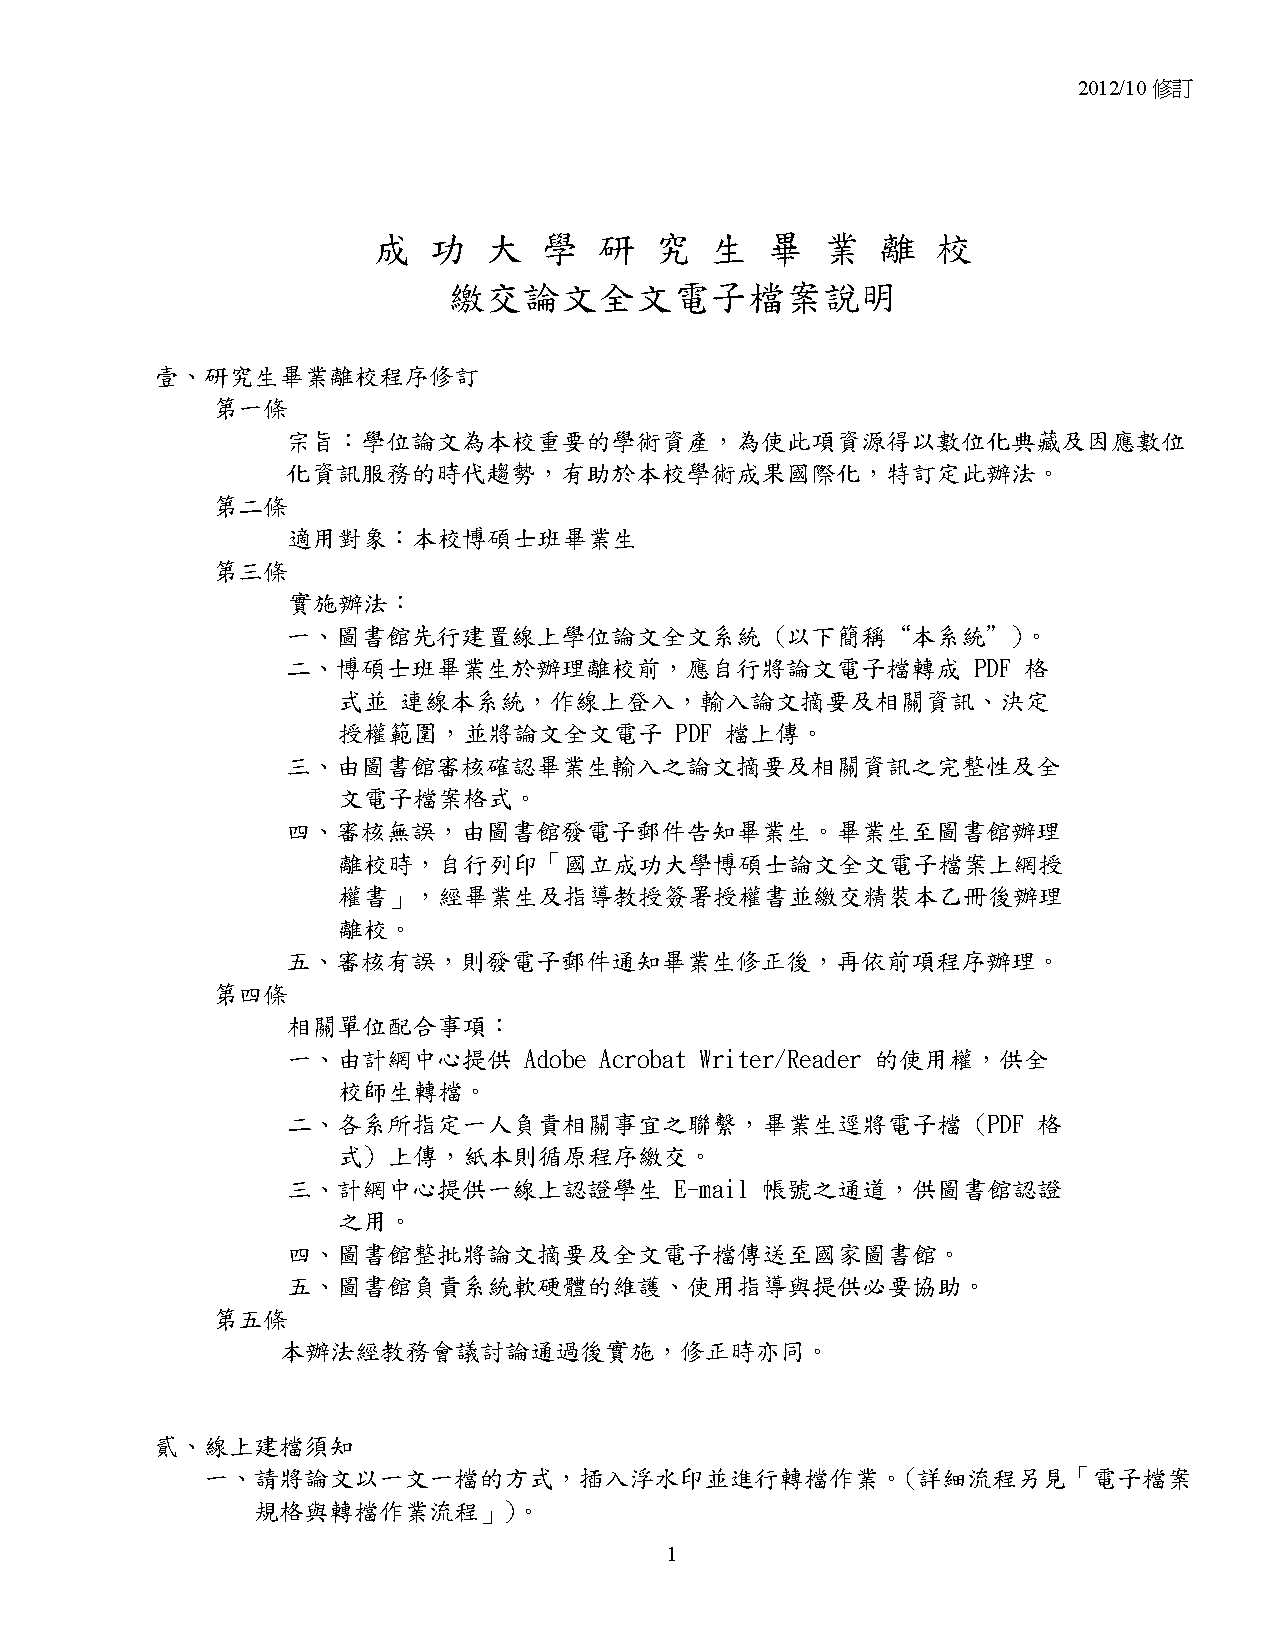
\includepdf[pages=-]{tutorial--pre-PH-fork/appendix/pdf/2012050004-a.pdf}
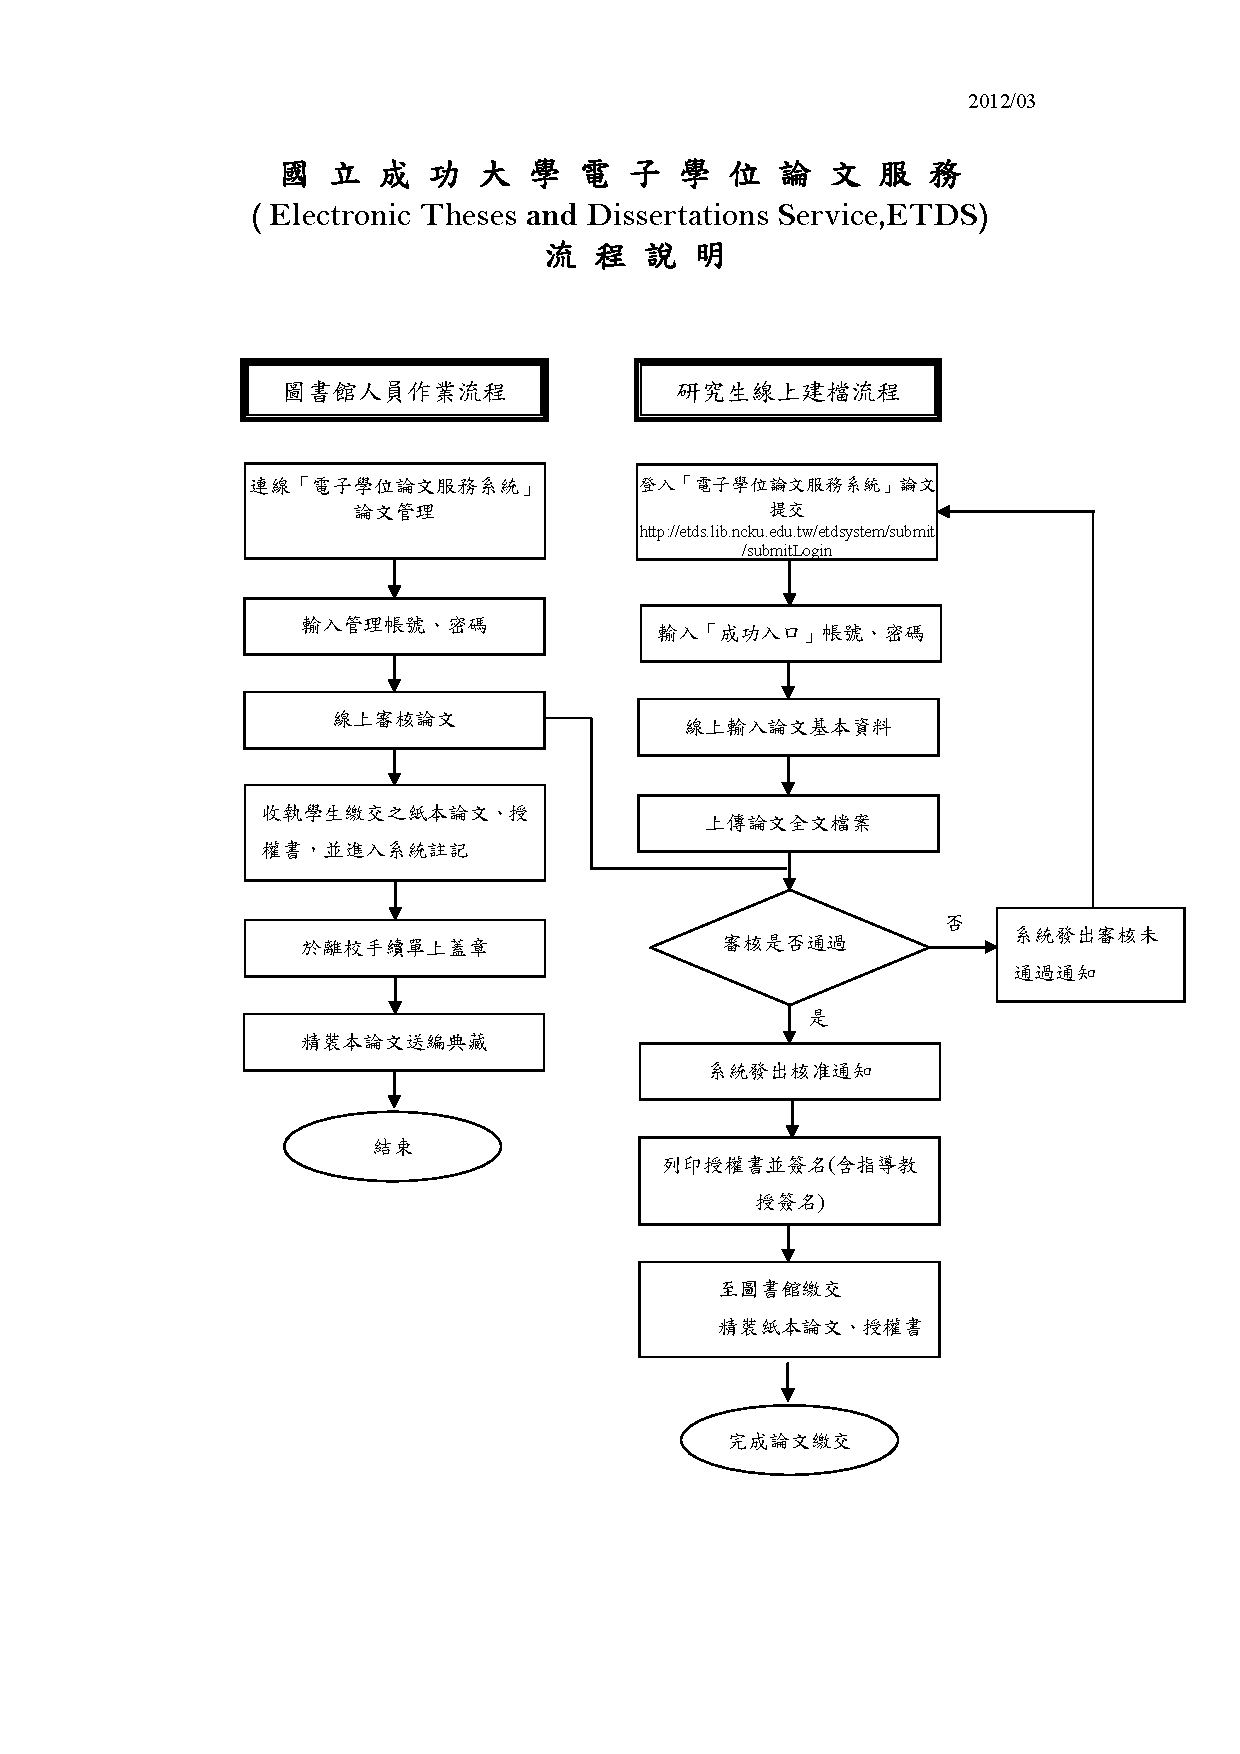
\includepdf[pages=-]{tutorial--pre-PH-fork/appendix/pdf/2012050006-a.pdf}

% ------------------------------------------------
\EndChapter
% ------------------------------------------------

% ------------------------------------------------
\StartChapter{各系所博碩士撰寫論文須知}{appendix:thesis-spec}
% ------------------------------------------------

這部份資料來源是使用'電子學位論文服務'提供'國立成功大學博碩士學位論文格式規範'\RefBib{web:ncku:thesis-need-to-know}.\\

\setboolean{@twoside}{false}
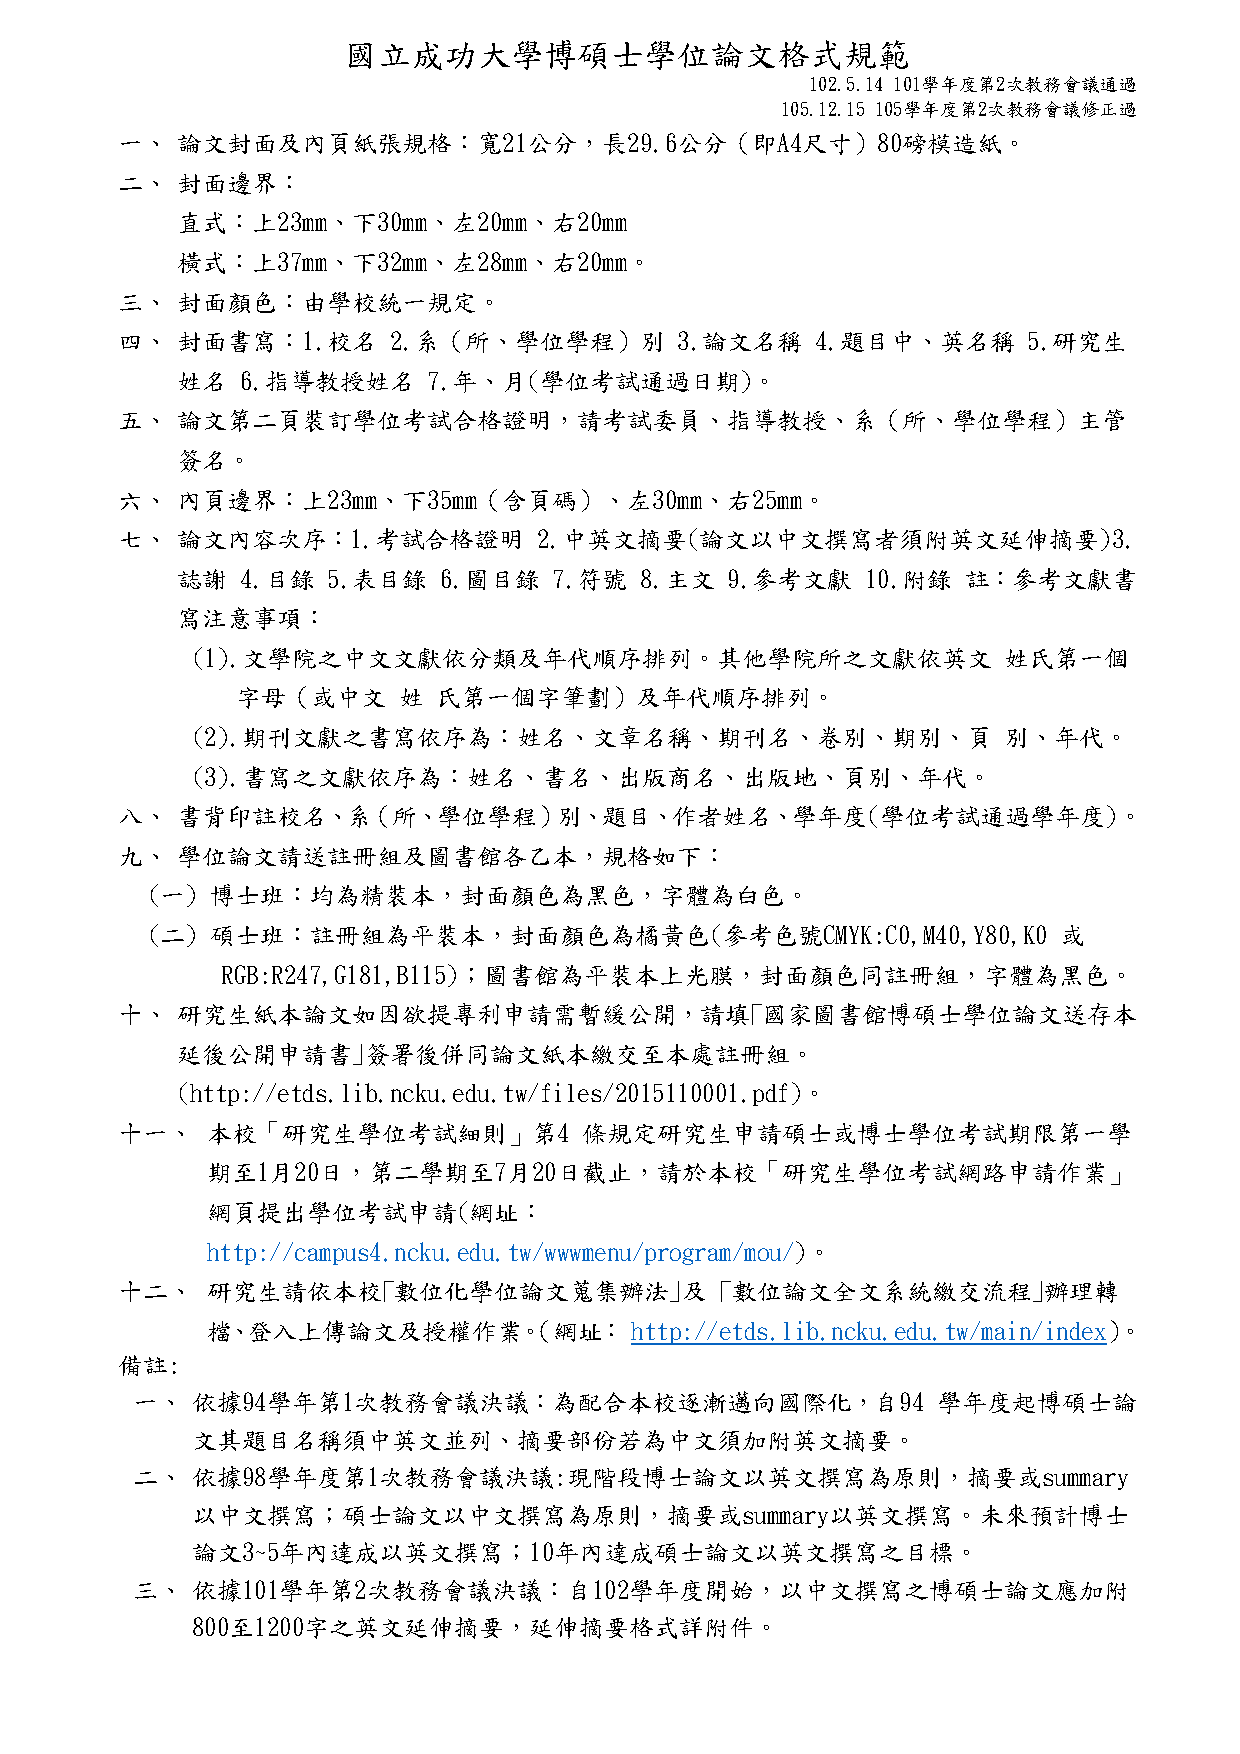
\includepdf[pages=-]{tutorial--pre-PH-fork/appendix/pdf/thesis-spec-a.pdf}

% ------------------------------------------------
\EndChapter
% ------------------------------------------------

% ------------------------------------------------
\StartChapter{電子論文上傳前檢查事項}{appendix:e-paper_upload}
% ------------------------------------------------

這部份資料來源是使用'電子學位論文服務'中的'電子論文上傳前檢查事項'的'2012090001.pdf'\RefBib{web:lib:upload-things-check}.\\

\setboolean{@twoside}{false}
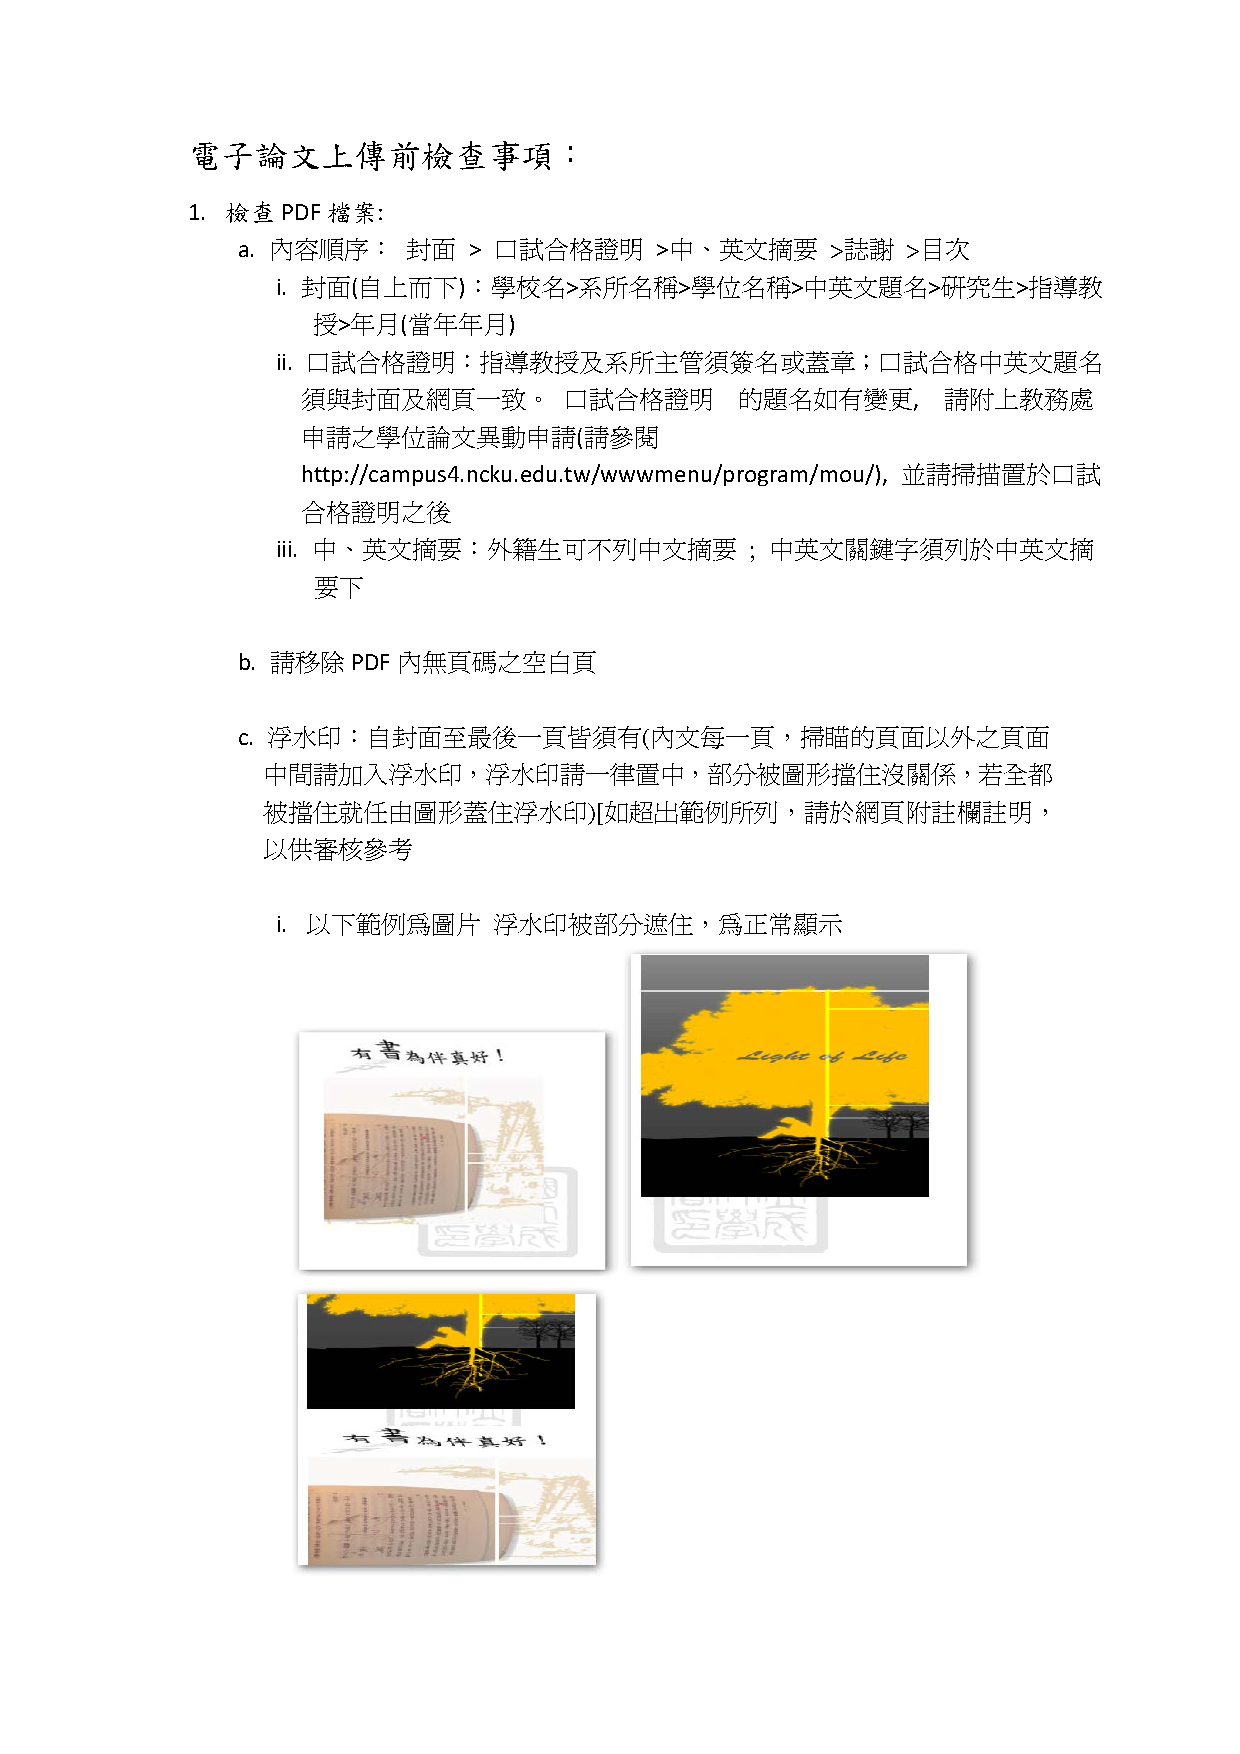
\includepdf[pages=-]{tutorial--pre-PH-fork/appendix/pdf/2012090001-a.pdf}

% ------------------------------------------------
\EndChapter
% ------------------------------------------------

% ------------------------------------------------
\StartChapter{論文提交說明}{appendix:e-paper_upload_ppt}
% ------------------------------------------------

這部份資料來源是使用'電子學位論文服務'提供的 '2016論文提交說明簡報檔'\RefBib{web:lib:2016-submit-ppt} 修改而成的, 只抽出使用本模版後, 還要做什麼的行為.\\

\setboolean{@twoside}{false}
\includepdf[pages=-]{tutorial--pre-PH-fork/appendix/pdf/2012050003-short-a}

% ------------------------------------------------
\EndChapter
% ------------------------------------------------

% ------------------------------------------------
\StartChapter{口試注意事項}
% ------------------------------------------------

這部份資料來源是使用本系資訊工程研究所系辦所提供的資料, 雖然內容主要針對本系, 但某些內容都是適合非本系的同學們.

\setboolean{@twoside}{false}
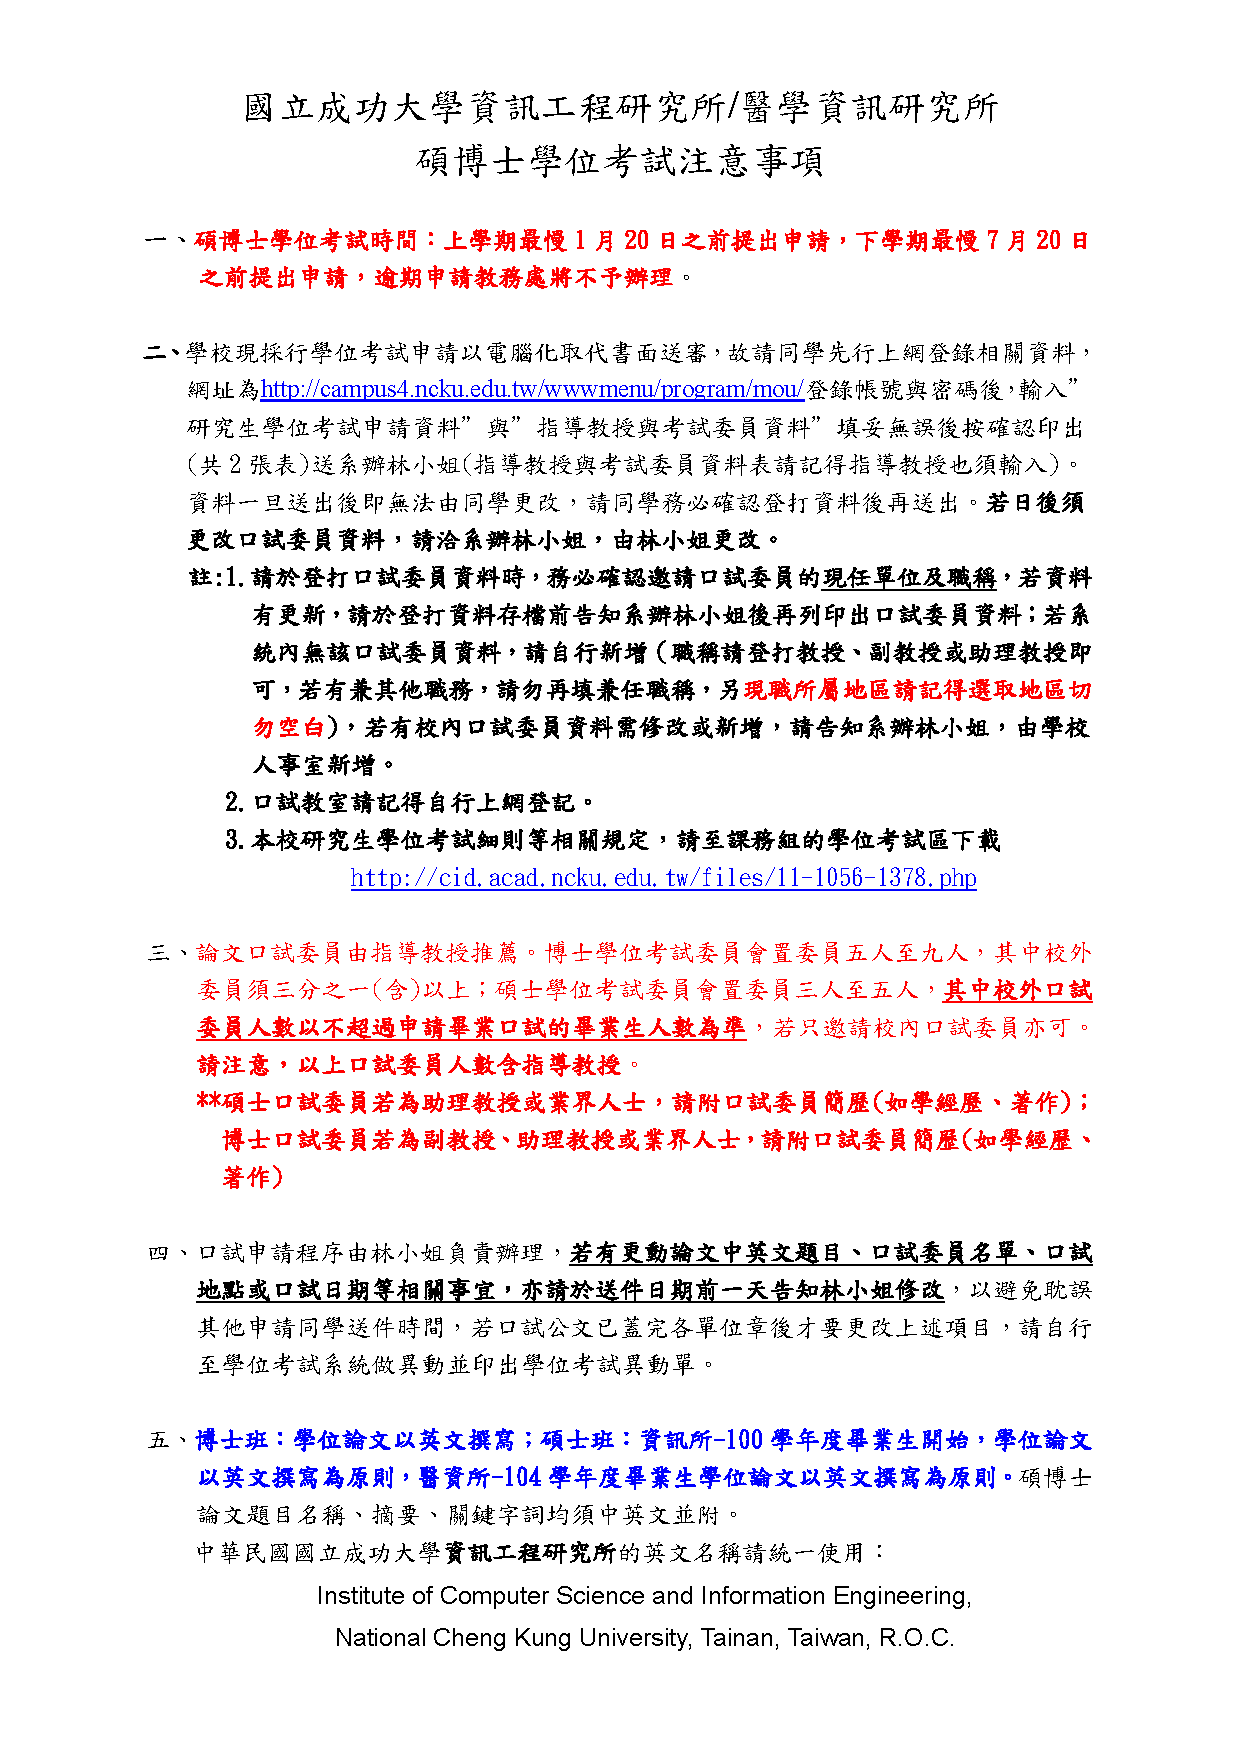
\includepdf[pages=-]{tutorial--pre-PH-fork/appendix/pdf/oral-1040616-a.pdf}

% ------------------------------------------------
\EndChapter
% ------------------------------------------------

% ------------------------------------------------
\StartChapter{常見問題Q\&A}{appendix:faq}
% ------------------------------------------------

這部份資料來源是使用'電子學位論文服務'提供的'FAQ'\RefBib{web:lib:ETDS-QA}, 用來補充其他Appendix沒提到的一些情報.\\

\setboolean{@twoside}{false}
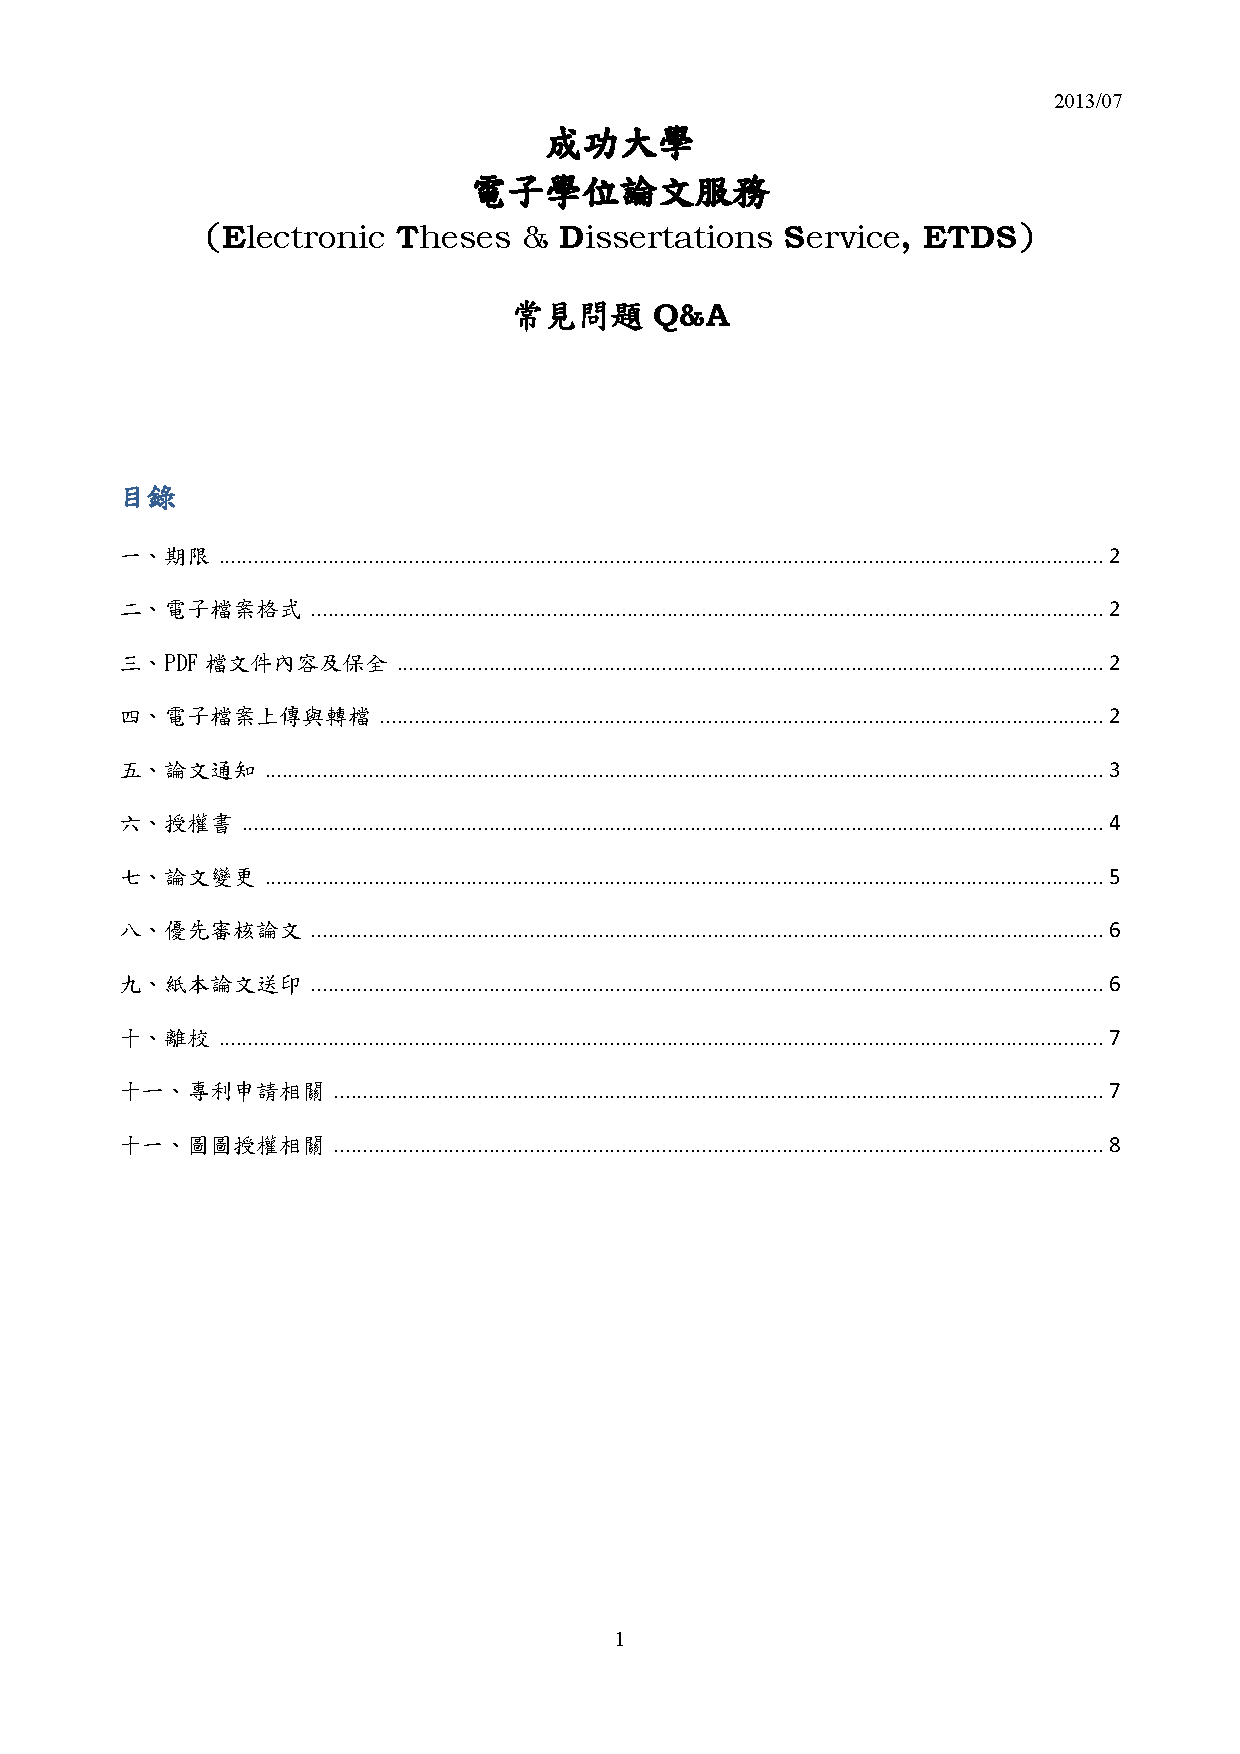
\includepdf[pages=-]{tutorial--pre-PH-fork/appendix/pdf/2012050009-a.pdf}

% ------------------------------------------------
\EndChapter
% ------------------------------------------------

% ------------------------------------------------
\StartChapter{LaTex Symbol寫法}{appendix:unicode-symbols}
% ------------------------------------------------

這部份資料來源是xeCJK的v3.3.4(2016/02/10)版本中提供的50頁有關所有Symbol的寫法, 極度值得同學們閱讀或在這邊找你所需的Symbols.\\

內容的說明方式為:\\
Symbol: 符號所顯示的樣子\\
USV: 以Unicode方式所代表的這個符號, 例如 `(' 的Unicode寫法為U+0028.\\
Description: 是這符號的名字.\\
Macro(s): 是LaTex使用這符號的寫法.\\

\textbf{P.S: }因為符號數量多, 沒法100\%保證全能使用.

\setboolean{@twoside}{false}
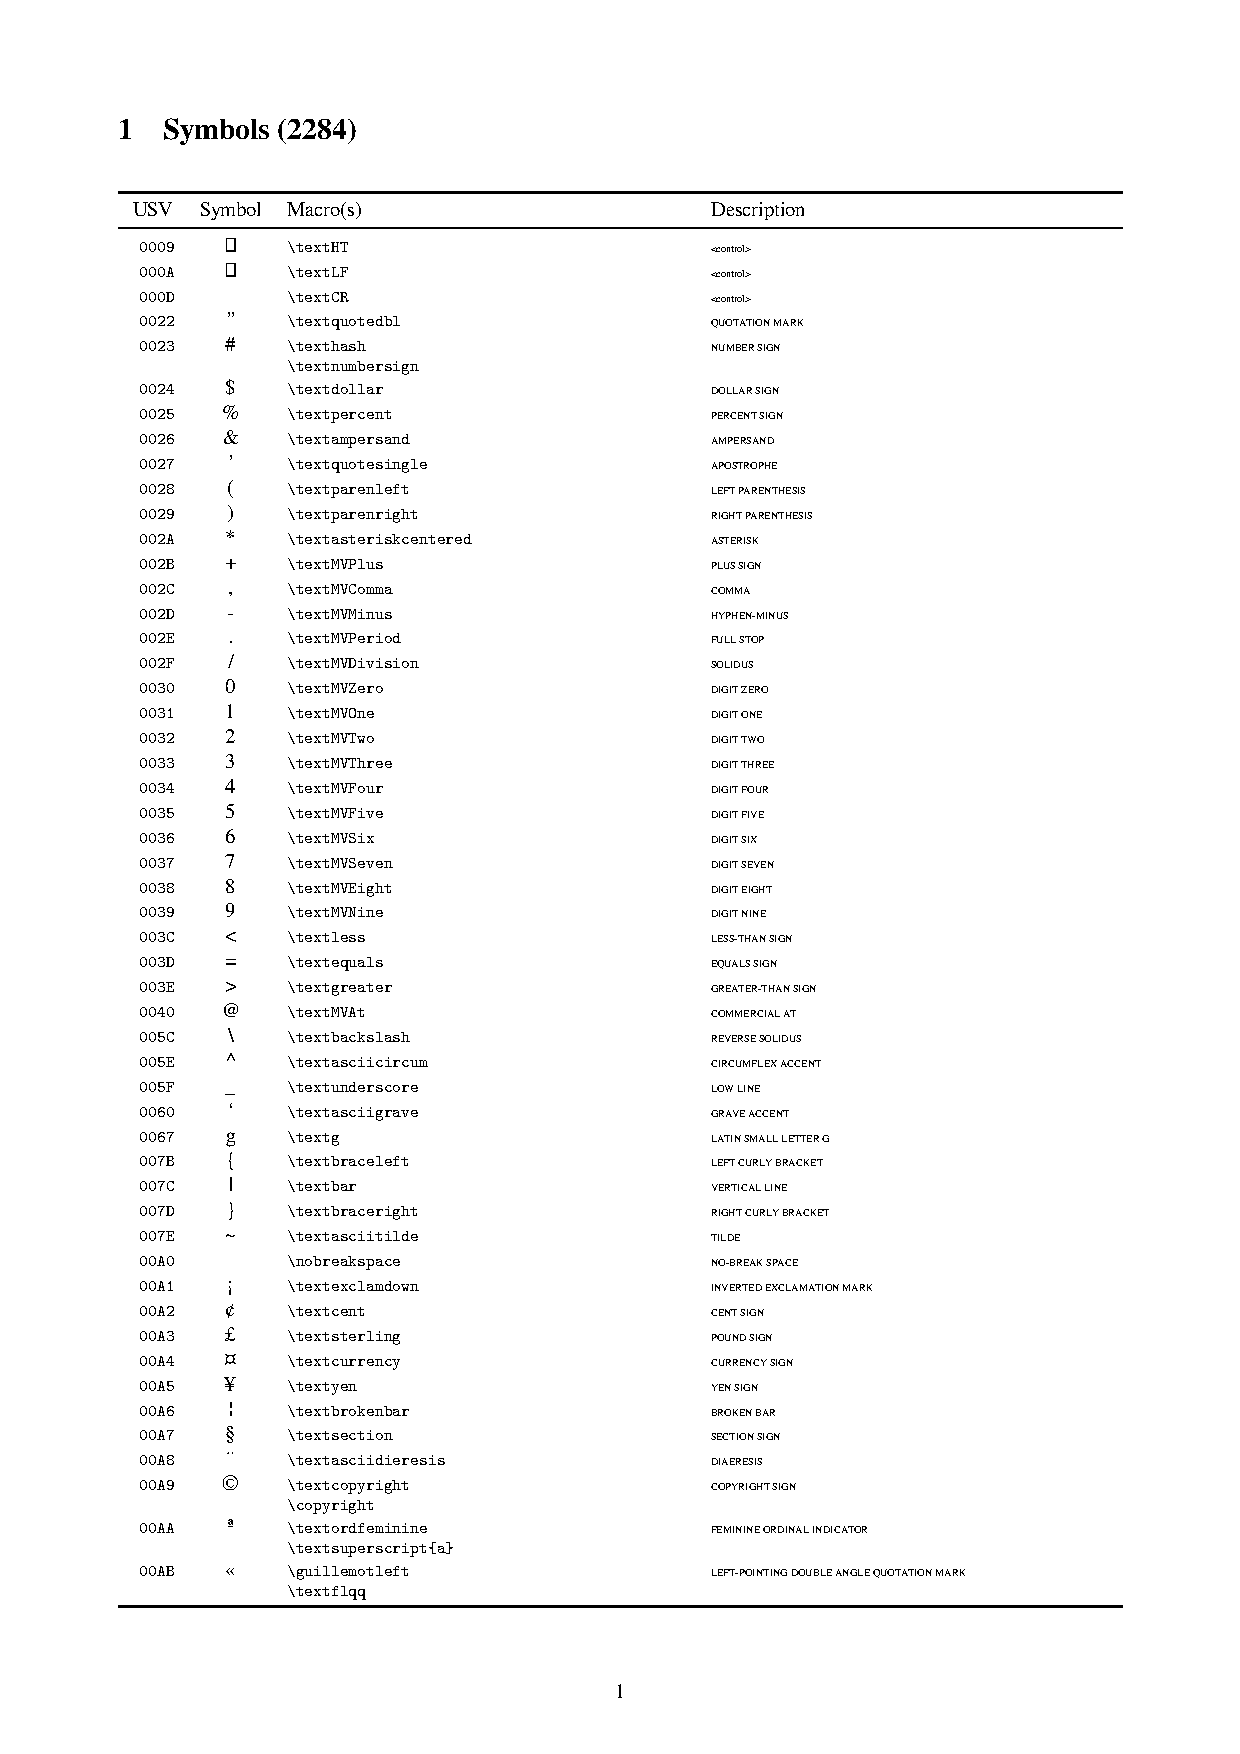
\includepdf[pages=-]{tutorial--pre-PH-fork/appendix/pdf/xunicode-symbols.pdf}

% ------------------------------------------------
\EndChapter
% ------------------------------------------------


% ------------------------------------------------
\EndAppendix
% ------------------------------------------------



% 用來對內容進行不同的設定測試用的測試頁
% ------------------------------------------------
\StartChapter{測試頁 Testing Pages}
% ------------------------------------------------

這邊是用來放置不同的內容來進行測試或設計樣版用的.

% 半形字元與全形字元
% ------------------------------------------------
%
% Reference from:
%
% 半形字元與全形字元
% <https://zh.wikipedia.org/wiki/%E5%85%A8%E5%BD%A2%E5%92%8C%E5%8D%8A%E5%BD%A2>
%
% ------------------------------------------------

\StartSection{半形字元與全形字元的比較 (ASCII字元)}
用來檢查半形/全形字元顯示正常\\

\begin{verbatim}
   全形    半形        |        全形    半形        |        全形    半形
   " "     " "                 !       !                  "       "
    #       #                  $       $                  %       %
    &       &                  '       '                  (       (
    )       )                  *       *                  +       +
    ,       ,                  -       -                  .       .
    /       /

    0       0                 1       1                  2       2
    3       3                 4       4                  5       5
    6       6                 7       7                  8       8
    9       9

    :       :                 ;       ;                  <       <
    =       =                 >       >                  ?       ?
    @       @

    A       A                 B       B                  C       C
    D       D                 E       E                  F       F
    G       G                 H       H                  I       I
    J       J                 K       K                  L       L
    M       M                 N       N                  O       O
    P       P                 Q       Q                  R       R
    S       S                 T       T                  U       U
    V       V                 W       W                  X       X
    Y       Y                 Z       Z

    [       [                 \       \                  ]       ]
    ^       ^                 _       _                  `       `

    a       a                 b       b                  c       c
    d       d                 e       e                  f       f
    g       g                 h       h                  i       i
    j       j                 k       k                  l       l
    m       m                 n       n                  o       o
    p       p                 q       q                  r       r
    s       s                 t       t                  u       u
    v       v                 w       w                  x       x
    y       y                 z       z

    {       {                 |       |                  }       }
    ~       ~
\end{verbatim}

% ------------------------------------------------


% 英文內容
% ------------------------------------------------

\newpage
\StartSection{英文內容 (只用段落來分段)}
用來看內容, 符號, 段距, 字元之間的距離等東西\\

NCKU offers an open learning environment characterized by classical Western and modern eastern landscape. NCKU has attracted numerous distinguished visitors around the world for its rich and welcoming campuses.

In addition to two off-university campuses, An-Nan and Gueiren, the main campus of NCKU consists of 7 satellite campuses adjacent to one another. NCKU occupies a total of more than 180 hectares of land, which tops many other universities in Taiwan. NCKU started out as having only one campus, Cheng Kung, but continued to expand to its current scale. Each campus in the major part of NCKU is closely interlinked and tightly developed as a city within the university.

NCKU's spirit of ``pristine practicality'' and its motto of ``intellectual development through persistent pursuit of knowledge'' have been intrinsic to the thick cultural heritage of the city of Tainan. While members of NCKU are well-integrated with one another, they also work independently. Patrons as NCKU enjoy abundant learning resources.

Through continuous evolution and progression, NCKU has become an active participant in global academia and has earned an excellent reputation in teaching and research. For example, NCKU has ranked the 256th in 2010 Academic Ranking of World Universities announced by Shanghai Jiaotong University and the 80th in 2011 Webometrics Ranking of World Universities published by Centre for Scientific Information and Documentation, Spain, only second to that of NTU, Todai and Kyodai in the Asian region.

% ------------------------------------------------

\newpage
\StartSection{英文內容 (只用強制斷行)}
用來看內容, 符號, 段距, 字元之間的距離等東西\\

NCKU offers an open learning environment characterized by classical Western and modern eastern landscape. NCKU has attracted numerous distinguished visitors around the world for its rich and welcoming campuses.\\
In addition to two off-university campuses, An-Nan and Gueiren, the main campus of NCKU consists of 7 satellite campuses adjacent to one another. NCKU occupies a total of more than 180 hectares of land, which tops many other universities in Taiwan. NCKU started out as having only one campus, Cheng Kung, but continued to expand to its current scale. Each campus in the major part of NCKU is closely interlinked and tightly developed as a city within the university.\\
NCKU's spirit of ``pristine practicality'' and its motto of ``intellectual development through persistent pursuit of knowledge'' have been intrinsic to the thick cultural heritage of the city of Tainan. While members of NCKU are well-integrated with one another, they also work independently. Patrons as NCKU enjoy abundant learning resources.\\
Through continuous evolution and progression, NCKU has become an active participant in global academia and has earned an excellent reputation in teaching and research. For example, NCKU has ranked the 256th in 2010 Academic Ranking of World Universities announced by Shanghai Jiaotong University and the 80th in 2011 Webometrics Ranking of World Universities published by Centre for Scientific Information and Documentation, Spain, only second to that of NTU, Todai and Kyodai in the Asian region.

% ------------------------------------------------

\newpage
\StartSection{英文內容 (段落 + 強制斷行)}
用來看內容, 符號, 段距, 字元之間的距離等東西\\

NCKU offers an open learning environment characterized by classical Western and modern eastern landscape. NCKU has attracted numerous distinguished visitors around the world for its rich and welcoming campuses.\\

In addition to two off-university campuses, An-Nan and Gueiren, the main campus of NCKU consists of 7 satellite campuses adjacent to one another. NCKU occupies a total of more than 180 hectares of land, which tops many other universities in Taiwan. NCKU started out as having only one campus, Cheng Kung, but continued to expand to its current scale. Each campus in the major part of NCKU is closely interlinked and tightly developed as a city within the university.\\

NCKU's spirit of ``pristine practicality'' and its motto of ``intellectual development through persistent pursuit of knowledge'' have been intrinsic to the thick cultural heritage of the city of Tainan. While members of NCKU are well-integrated with one another, they also work independently. Patrons as NCKU enjoy abundant learning resources.\\

Through continuous evolution and progression, NCKU has become an active participant in global academia and has earned an excellent reputation in teaching and research. For example, NCKU has ranked the 256th in 2010 Academic Ranking of World Universities announced by Shanghai Jiaotong University and the 80th in 2011 Webometrics Ranking of World Universities published by Centre for Scientific Information and Documentation, Spain, only second to that of NTU, Todai and Kyodai in the Asian region.

% ------------------------------------------------


% 中文內容
% ------------------------------------------------

\newpage
\StartSection{中文內容 (只用段落來分段)}
用來看內容, 符號, 段距, 字元之間的距離等東西\\

本校創校於西元1931年(昭和6年,民國20年)1月15日,原名為「臺南高等工業學校」;1944年(昭和19年,民國33年)改稱為「臺南工業專門學校」。民國34年臺灣光復。本校於民國35年2月改制為「臺灣省立臺南工業專科學校」,由王石安博士擔任校長;35年10月改制為「臺灣省立工學院」,仍由王石安博士擔任校長。彼時僅有成功校區,39年增購勝利校區。41年2月,由秦大鈞博士接任校長。

45年8月,本校改制為「臺灣省立成功大學」,仍由秦大鈞博士擔任校長;同時增設文理學院及商學院。46年8月,由閻振興博士接任校長。54年1月,由羅雲平博士接任校長。55年增購光復校區。58年10月,將文理學院分為文學院及理學院。60年8月,改制為「國立成功大學」,並由倪超博士接任校長;同年增購建國校區。67年8月,由王唯農博士接任校長。

69年8月,夏漢民博士接任校長;同年將商學院更名為管理學院。72年8月,增設醫學院,並增購自強校區及敬業校區。74年增購力行校區部分校地。76年增購歸仁校區,設置航空太空實驗場。77年6月本校醫學院附設醫院正式營運。77年8月,馬哲儒博士接任校長。80年增購自強校區北半部。82年陸續增購台南市「文大五」用地,闢為本校安南校區。

83年8月,吳京院士接任校長。吳校長於85年6月入閣擔任教育部長,由副校長黃定加博士代理校長。86年2月,翁政義博士接任校長。86年8月增設社會科學院。88年完成收購安南校區全部校地;同年6月增購原陸軍八○四醫院用地(91年6月完成撥用手續)。翁校長於89年5月出任國科會主委,由副校長翁鴻山博士代理校長。90年2月,高強博士接任校長。92年8月,增設電機資訊學院、規劃與設計學院。94年7月,本校配合國軍斗六醫院精實案,接管該院營運權,設置為雲林縣斗六校區,並改制為本校醫學院附設醫院斗六分院。94年8月,增設生物科學與科技學院。94年10月,本校得到教育部的肯定,獲選為「發展國際一流大學及頂尖研究中心計畫」的兩所重點大學之一。

96年2月,賴明詔院士接任校長,97年2月教育部公佈「發展國際一流大學及頂尖研究中心計畫」第二梯次的審議結果,本校繼續獲得教育部的肯定與補助,積極朝國際一流大學的目標邁進。97年10月增購歸仁校區北側台糖土地(正式登記為本校管有)。100年2月,黃煌煇博士接任校長。100年4月本校獲得教育部第二期頂尖大學計畫補助,持續朝國際一流大學的目標邁進。104年2月,蘇慧貞博士接任校長。

% ------------------------------------------------

\newpage
\StartSection{中文內容 (只用強制斷行)}
用來看內容, 符號, 段距, 字元之間的距離等東西\\

本校創校於西元1931年(昭和6年,民國20年)1月15日,原名為「臺南高等工業學校」;1944年(昭和19年,民國33年)改稱為「臺南工業專門學校」。民國34年臺灣光復。本校於民國35年2月改制為「臺灣省立臺南工業專科學校」,由王石安博士擔任校長;35年10月改制為「臺灣省立工學院」,仍由王石安博士擔任校長。彼時僅有成功校區,39年增購勝利校區。41年2月,由秦大鈞博士接任校長。\\
45年8月,本校改制為「臺灣省立成功大學」,仍由秦大鈞博士擔任校長;同時增設文理學院及商學院。46年8月,由閻振興博士接任校長。54年1月,由羅雲平博士接任校長。55年增購光復校區。58年10月,將文理學院分為文學院及理學院。60年8月,改制為「國立成功大學」,並由倪超博士接任校長;同年增購建國校區。67年8月,由王唯農博士接任校長。\\
69年8月,夏漢民博士接任校長;同年將商學院更名為管理學院。72年8月,增設醫學院,並增購自強校區及敬業校區。74年增購力行校區部分校地。76年增購歸仁校區,設置航空太空實驗場。77年6月本校醫學院附設醫院正式營運。77年8月,馬哲儒博士接任校長。80年增購自強校區北半部。82年陸續增購台南市「文大五」用地,闢為本校安南校區。\\
83年8月,吳京院士接任校長。吳校長於85年6月入閣擔任教育部長,由副校長黃定加博士代理校長。86年2月,翁政義博士接任校長。86年8月增設社會科學院。88年完成收購安南校區全部校地;同年6月增購原陸軍八○四醫院用地(91年6月完成撥用手續)。翁校長於89年5月出任國科會主委,由副校長翁鴻山博士代理校長。90年2月,高強博士接任校長。92年8月,增設電機資訊學院、規劃與設計學院。94年7月,本校配合國軍斗六醫院精實案,接管該院營運權,設置為雲林縣斗六校區,並改制為本校醫學院附設醫院斗六分院。94年8月,增設生物科學與科技學院。94年10月,本校得到教育部的肯定,獲選為「發展國際一流大學及頂尖研究中心計畫」的兩所重點大學之一。\\
96年2月,賴明詔院士接任校長,97年2月教育部公佈「發展國際一流大學及頂尖研究中心計畫」第二梯次的審議結果,本校繼續獲得教育部的肯定與補助,積極朝國際一流大學的目標邁進。97年10月增購歸仁校區北側台糖土地(正式登記為本校管有)。100年2月,黃煌煇博士接任校長。100年4月本校獲得教育部第二期頂尖大學計畫補助,持續朝國際一流大學的目標邁進。104年2月,蘇慧貞博士接任校長。

% ------------------------------------------------

\newpage
\StartSection{中文內容 (段落 + 強制斷行)}
用來看內容, 符號, 段距, 字元之間的距離等東西\\

本校創校於西元1931年(昭和6年,民國20年)1月15日,原名為「臺南高等工業學校」;1944年(昭和19年,民國33年)改稱為「臺南工業專門學校」。民國34年臺灣光復。本校於民國35年2月改制為「臺灣省立臺南工業專科學校」,由王石安博士擔任校長;35年10月改制為「臺灣省立工學院」,仍由王石安博士擔任校長。彼時僅有成功校區,39年增購勝利校區。41年2月,由秦大鈞博士接任校長。\\

45年8月,本校改制為「臺灣省立成功大學」,仍由秦大鈞博士擔任校長;同時增設文理學院及商學院。46年8月,由閻振興博士接任校長。54年1月,由羅雲平博士接任校長。55年增購光復校區。58年10月,將文理學院分為文學院及理學院。60年8月,改制為「國立成功大學」,並由倪超博士接任校長;同年增購建國校區。67年8月,由王唯農博士接任校長。\\

69年8月,夏漢民博士接任校長;同年將商學院更名為管理學院。72年8月,增設醫學院,並增購自強校區及敬業校區。74年增購力行校區部分校地。76年增購歸仁校區,設置航空太空實驗場。77年6月本校醫學院附設醫院正式營運。77年8月,馬哲儒博士接任校長。80年增購自強校區北半部。82年陸續增購台南市「文大五」用地,闢為本校安南校區。\\

83年8月,吳京院士接任校長。吳校長於85年6月入閣擔任教育部長,由副校長黃定加博士代理校長。86年2月,翁政義博士接任校長。86年8月增設社會科學院。88年完成收購安南校區全部校地;同年6月增購原陸軍八○四醫院用地(91年6月完成撥用手續)。翁校長於89年5月出任國科會主委,由副校長翁鴻山博士代理校長。90年2月,高強博士接任校長。92年8月,增設電機資訊學院、規劃與設計學院。94年7月,本校配合國軍斗六醫院精實案,接管該院營運權,設置為雲林縣斗六校區,並改制為本校醫學院附設醫院斗六分院。94年8月,增設生物科學與科技學院。94年10月,本校得到教育部的肯定,獲選為「發展國際一流大學及頂尖研究中心計畫」的兩所重點大學之一。\\

96年2月,賴明詔院士接任校長,97年2月教育部公佈「發展國際一流大學及頂尖研究中心計畫」第二梯次的審議結果,本校繼續獲得教育部的肯定與補助,積極朝國際一流大學的目標邁進。97年10月增購歸仁校區北側台糖土地(正式登記為本校管有)。100年2月,黃煌煇博士接任校長。100年4月本校獲得教育部第二期頂尖大學計畫補助,持續朝國際一流大學的目標邁進。104年2月,蘇慧貞博士接任校長。

% ------------------------------------------------


% 混合的中英文內容
% ------------------------------------------------

\newpage
\StartSection{混合的中英文內容 (只用段落來分段)}
用來看內容, 符號, 段距, 字元之間的距離等東西\\

Google公司(英語:Google Inc.; 中文:穀歌[3]、穀歌[4]、科高[5]), 是一家美國的跨國科技企業, 業務範圍涵蓋互聯網搜索、雲計算、廣告技術等領域, 開發並提供大量基於互聯網的產品與服務[6], 其主要利潤來自於AdWords等廣告服務[7][8].

\begin{description}
\item [Google] Google由在斯坦福大學攻讀理工博士的拉裡•佩奇和謝爾蓋•布林共同創建, 因此兩人也被稱為``Google Guys''[9][10][11]. 1998年9月4日, Google以私營公司的形式創立, 目的是設計並管理互聯網搜尋引擎``Google搜索''. 2004年8月19日, Google公司在納斯達克上市, 後來被稱為``三駕馬車''的公司兩位共同創始人與出任首席執行官的埃裡克•施密特在此時承諾:共同在Google工作至少二十年, 即至2024年止[12].

\item [Google]\hfill\\ Google由在斯坦福大學攻讀理工博士的拉裡•佩奇和謝爾蓋•布林共同創建, 因此兩人也被稱為``Google Guys''[9][10][11]. 1998年9月4日, Google以私營公司的形式創立, 目的是設計並管理互聯網搜尋引擎``Google搜索''. 2004年8月19日, Google公司在納斯達克上市, 後來被稱為``三駕馬車''的公司兩位共同創始人與出任首席執行官的埃裡克•施密特在此時承諾:共同在Google工作至少二十年, 即至2024年止[12].

\item Google的宗旨是``整合全球範圍的資訊, 使人人皆可訪問並從中受益''(To organize the world's information and make it universally accessible and useful)[13]; 而非正式的口號則為``不作惡''(Don't be evil), 由工程師阿米特•派特爾(Amit Patel)所創[14], 並得到了保羅•布赫海特的支持[15][16]. Google公司的總部稱為``Googleplex'', 位於美國加州聖克拉拉縣的山景城. 2011年4月, 佩奇接替施密特擔任首席執行官[17].

\item 在2015年8月, Google進行宣佈資產重組. 重組後, Google劃歸新成立的Alphabet底下. 同時, 此舉把Google旗下的核心搜索和廣告業務與Google無人車等新興業務分離開來[18].
\end{description}

據估計, Google在全世界的資料中心內運營著上百萬台的伺服器, [19]每天處理數以億計的搜索請求[20]和約二十四PB使用者生成的資料. [21][22][23][24] Google自創立起開始的快速成長同時也帶動了一系列的產品研發、並購事項與合作關係, 而不僅僅是公司核心的網路搜索業務. Google公司提供豐富的線上軟體服務, 如雲端硬碟、Gmail電子郵件, 包括Orkut、Google Buzz以及Google+在內的社交網路服務. Google的產品同時也以應用軟體的形式進入使用者桌面, 例如Google Chrome網頁流覽器、Picasa圖片整理與編輯軟體、Google Talk即時通訊工具等. 另外, Google還進行了移動設備的Android作業系統以及Google Chrome OS作業系統的開發. [25]

資訊分析網站Alexa資料顯示, Google的主功能變數名稱google.com是全世界訪問量最高的網站, Google搜索在其他國家或地區域名下的多個網站(google.co.in、google.de、google.com.hk等等), 及旗下的YouTube、Blogger、Orkut等的訪問量都在前一百名之內. [26]其中, 社交網路服務Orkut於2014年9月關閉. [27]

Facebook(原本稱作thefacebook)是一家位於美國加州聖馬刁郡門洛派克市的線上社交網路服務網站. 其名稱的靈感來自美國高中提供給學生包含照片和聯絡資料的通訊錄(或稱花名冊)暱稱「face book」[6][7].

除了文字訊息之外, 使用者可傳送圖片、影片和聲音媒體訊息(現在也可以傳送其他檔案類型如.doc,.docx,.xls,.xlsx等, 但是.exe可能會被禁止傳送)給其他使用者, 以及透過整合的地圖功能分享使用者的所在位置. Facebook是在2004年2月4日由馬克•紮克伯格與他的哈佛大學室友們所創立[8]. Facebook的會員最初只限於哈佛學生加入, 但後來逐漸擴展到其他在波士頓區域的同學也能使用, 包括一些常春藤名校、MIT、紐約大學、史丹福大學等. 接著逐漸支援讓其他大學和高中學生加入, 並在最後開放給任何13歲或以上的人使用.  現在Facebook允許任何聲明自己年滿13歲的使用者註冊[9].

使用者必須註冊才能使用Facebook, 註冊後他們可以創建個人檔案、將其他使用者加為好友、傳遞訊息, 並在其他使用者更新個人檔案時獲得自動通知. 此外使用者也可以加入有相同興趣的群組, 這些群組依據工作地點、學校或其他特性分類. 使用者亦可將朋友分別加入不同的列表中管理, 例如「同事」或「摯友」等. 截至2012年9月, Facebook內已有超過十幾億個活躍使用者[10], 其中約有9\%的不實使用者[11]. 截至2012年, Facebook每年共產生180拍位元組(PB)的資料, 並以每24小時0.5拍位元元組的速度增加[12]. 統計顯示, Facebook上每天上傳3億5千萬張圖片. [13]

Facebook創始人馬克•紮克伯格是世界上最著名的CEO之一. 而馬克•紮克伯格曾經的朋友與商業合作夥伴愛德華多•薩維林在新加坡亦十分知名[14].

Google公司(英語:Google Inc.; 中文:穀歌[3]、穀歌[4]、科高[5]), 是一家美國的跨國科技企業, 業務範圍涵蓋互聯網搜索、雲計算、廣告技術等領域, 開發並提供大量基於互聯網的產品與服務[6], 其主要利潤來自於AdWords等廣告服務[7][8].

\begin{itemize}
\item Google由在斯坦福大學攻讀理工博士的拉裡•佩奇和謝爾蓋•布林共同創建, 因此兩人也被稱為``Google Guys''[9][10][11]. 1998年9月4日, Google以私營公司的形式創立, 目的是設計並管理互聯網搜尋引擎``Google搜索''. 2004年8月19日, Google公司在納斯達克上市, 後來被稱為``三駕馬車''的公司兩位共同創始人與出任首席執行官的埃裡克•施密特在此時承諾:共同在Google工作至少二十年, 即至2024年止[12].

\item Google的宗旨是``整合全球範圍的資訊, 使人人皆可訪問並從中受益''(To organize the world's information and make it universally accessible and useful)[13];
\begin{itemize}
\item Google的宗旨是``整合全球範圍的資訊, 使人人皆可訪問並從中受益''(To organize the world's information and make it universally accessible and useful)[13]; 而非正式的口號則為``不作惡''(Don't be evil), 由工程師阿米特•派特爾(Amit Patel)所創[14], 並得到了保羅•布赫海特的支持[15][16]. Google公司的總部稱為``Googleplex'', 位於美國加州聖克拉拉縣的山景城. 2011年4月, 佩奇接替施密特擔任首席執行官[17].
\item Google的宗旨是``整合全球範圍的資訊, 使人人皆可訪問並從中受益''(To organize the world's information and make it universally accessible and useful)[13].
\item Google公司的總部稱為``Googleplex'', 位於美國加州聖克拉拉縣的山景城. 2011年4月, 佩奇接替施密特擔任首席執行官[17].
\end{itemize}

\item 在2015年8月, Google進行宣佈資產重組. 重組後, Google劃歸新成立的Alphabet底下. 同時, 此舉把Google旗下的核心搜索和廣告業務與Google無人車等新興業務分離開來[18].
\end{itemize}

據估計, Google在全世界的資料中心內運營著上百萬台的伺服器, [19]每天處理數以億計的搜索請求[20]和約二十四PB使用者生成的資料. [21][22][23][24] Google自創立起開始的快速成長同時也帶動了一系列的產品研發、並購事項與合作關係, 而不僅僅是公司核心的網路搜索業務. Google公司提供豐富的線上軟體服務, 如雲端硬碟、Gmail電子郵件, 包括Orkut、Google Buzz以及Google+在內的社交網路服務. Google的產品同時也以應用軟體的形式進入使用者桌面, 例如Google Chrome網頁流覽器、Picasa圖片整理與編輯軟體、Google Talk即時通訊工具等. 另外, Google還進行了移動設備的Android作業系統以及Google Chrome OS作業系統的開發. [25]

資訊分析網站Alexa資料顯示, Google的主功能變數名稱google.com是全世界訪問量最高的網站, Google搜索在其他國家或地區域名下的多個網站(google.co.in、google.de、google.com.hk等等), 及旗下的YouTube、Blogger、Orkut等的訪問量都在前一百名之內. [26]其中, 社交網路服務Orkut於2014年9月關閉. [27]

Facebook(原本稱作thefacebook)是一家位於美國加州聖馬刁郡門洛派克市的線上社交網路服務網站. 其名稱的靈感來自美國高中提供給學生包含照片和聯絡資料的通訊錄(或稱花名冊)暱稱「face book」[6][7].
\begin{enumerate}
\item 除了文字訊息之外, 使用者可傳送圖片、影片和聲音媒體訊息(現在也可以傳送其他檔案類型如.doc,.docx,.xls,.xlsx等, 但是.exe可能會被禁止傳送)給其他使用者, 以及透過整合的地圖功能分享使用者的所在位置.

\item Facebook是在2004年2月4日由馬克•紮克伯格與他的哈佛大學室友們所創立[8]. Facebook的會員最初只限於哈佛學生加入, 但後來逐漸擴展到其他在波士頓區域的同學也能使用, 包括一些常春藤名校、MIT、紐約大學、史丹福大學等.

\item 接著逐漸支援讓其他大學和高中學生加入, 並在最後開放給任何13歲或以上的人使用.  現在Facebook允許任何聲明自己年滿13歲的使用者註冊[9].
\end{enumerate}
使用者必須註冊才能使用Facebook, 註冊後他們可以創建個人檔案、將其他使用者加為好友、傳遞訊息, 並在其他使用者更新個人檔案時獲得自動通知. 此外使用者也可以加入有相同興趣的群組, 這些群組依據工作地點、學校或其他特性分類. 使用者亦可將朋友分別加入不同的列表中管理, 例如「同事」或「摯友」等. 截至2012年9月, Facebook內已有超過十幾億個活躍使用者[10], 其中約有9\%的不實使用者[11]. 截至2012年, Facebook每年共產生180拍位元組(PB)的資料, 並以每24小時0.5拍位元元組的速度增加[12]. 統計顯示, Facebook上每天上傳3億5千萬張圖片. [13]

Facebook創始人馬克•紮克伯格是世界上最著名的CEO之一. 而馬克•紮克伯格曾經的朋友與商業合作夥伴愛德華多•薩維林在新加坡亦十分知名[14].

% ------------------------------------------------


% 表格
% ------------------------------------------------

\newpage
\StartSection{Table使用透明度}

\vspace{3.0cm}

\InsertTable
  [caption={opacity使用預設}]
  {
    \begin{tabular}{llll}
    \hline
    Engine &  &  & OPEL Astra C16SE \\ \hline
    Displacement (cc) &  &  & 1598 \\
    Bore x stroke(mm x mm) &  &  & 79 x 81.5 \\
    Value mechanism &  &  & SOHC \\
    Number of valves &  &  & Intake 4, exhaust 4 \\
    Compression ratio &  &  & 9.8:1 \\
    Torque &  &  & 135/3400 Nm/rpm \\
    Power &  &  & 74/5800 kW/rpm \\
    Ignition sequence &  &  & 1-3-4-2 \\
    Spark plug &  &  & BPR6ES \\
    Fuel &  &  & 95 unleaded gasoline \\
    Cylinder arrangment &  &  & In-line 4 cylinders \\ \hline
    \end{tabular}
  } % End of  \InsertTable{}

  \InsertTable
    [caption={測試opacity=0.4},
      opacity=0.4]
    {
      \begin{tabular}{|c|c|c|c|c|c|c|c|c|c|c|c|c|c|c|c|}
      \hline
       & Col 1 & Col 2 & Col 3 & Col 4 & Col 5 & Col 6 & Col 7 & Col 8 & Col 9 & Col 10 & Col 11 & Col 12 & Col 13 & Col 14 \\ \hline
      Row 1 & Value & Value & Value & Value & Value & Value & Value & Value & Value & Value & Value & Value & Value & Value \\ \hline
      Row 2 & Value & Value & Value & Value & Value & Value & Value & Value & Value & Value & Value & Value & Value & Value \\ \hline
      Row 3 & Value & Value & Value & Value & Value & Value & Value & Value & Value & Value & Value & Value & Value & Value \\ \hline
      Row 4 & Value & Value & Value & Value & Value & Value & Value & Value & Value & Value & Value & Value & Value & Value \\ \hline
      \end{tabular}
  } % End of  \InsertTable{}

% ------------------------------------------------

\newpage
\StartSection{Table測試寬度}

  \InsertTable
    [caption={不進行寬度設定, 應超出頁面}]
    {
      \begin{tabular}{|c|c|c|c|c|c|c|c|c|c|c|c|c|c|c|c|}
      \hline
       & Col 1 & Col 2 & Col 3 & Col 4 & Col 5 & Col 6 & Col 7 & Col 8 & Col 9 & Col 10 & Col 11 & Col 12 & Col 13 & Col 14 \\ \hline
      Row 1 & Value & Value & Value & Value & Value & Value & Value & Value & Value & Value & Value & Value & Value & Value \\ \hline
      Row 2 & Value & Value & Value & Value & Value & Value & Value & Value & Value & Value & Value & Value & Value & Value \\ \hline
      Row 3 & Value & Value & Value & Value & Value & Value & Value & Value & Value & Value & Value & Value & Value & Value \\ \hline
      Row 4 & Value & Value & Value & Value & Value & Value & Value & Value & Value & Value & Value & Value & Value & Value \\ \hline
      \end{tabular}
  } % End of  \InsertTable{}

  \InsertTable
    [scale=0.9,
      caption={表格寬度設定scale=0.9}]
    {
      \begin{tabular}{|c|c|c|c|c|c|c|c|c|c|c|c|c|c|c|c|}
      \hline
       & Col 1 & Col 2 & Col 3 & Col 4 & Col 5 & Col 6 & Col 7 & Col 8 & Col 9 & Col 10 & Col 11 & Col 12 & Col 13 & Col 14 \\ \hline
      Row 1 & Value & Value & Value & Value & Value & Value & Value & Value & Value & Value & Value & Value & Value & Value \\ \hline
      Row 2 & Value & Value & Value & Value & Value & Value & Value & Value & Value & Value & Value & Value & Value & Value \\ \hline
      Row 3 & Value & Value & Value & Value & Value & Value & Value & Value & Value & Value & Value & Value & Value & Value \\ \hline
      Row 4 & Value & Value & Value & Value & Value & Value & Value & Value & Value & Value & Value & Value & Value & Value \\ \hline
      \end{tabular}
  } % End of  \InsertTable{}

% ------------------------------------------------


% ------------------------------------------------

\newpage
\StartSection{Figure使用透明度}

\vspace{2.0cm}

\InsertFigure
  [scale=0.5,
    caption={opacity使用預設}]
  {tutorial--pre-PH-fork/abstract/pic/extended-abstract-2.jpg}

\InsertFigure
  [scale=0.5,
    caption={測試opacity=0.4},
    opacity=0.4]
  {tutorial--pre-PH-fork/abstract/pic/extended-abstract-2.jpg}

\newpage

\EmptyLine
\vspace{7.0cm}

    \InsertFigures
    [caption={opacity使用預設}] %
    {
      {tutorial--pre-PH-fork/how-to/write/figure/pic/CC-BY-NC.png}
    }%
    {
      {tutorial--pre-PH-fork/how-to/write/figure/pic/CC-BY-NC-ND.png}
    }

\vspace{1.0cm}

    \InsertFigures
    [caption={測試opacity=0.4},
    opacity=0.4]
    {
      {tutorial--pre-PH-fork/how-to/write/figure/pic/CC-BY-NC.png}
    }%
    {
      {tutorial--pre-PH-fork/how-to/write/figure/pic/CC-BY-NC-ND.png}
    }

% ------------------------------------------------


% ------------------------------------------------

\newpage
\StartSection{Equation}

\EquationBegin
  x = &a + b + c + \\
  &d + e + f + g + \\
  &h + i + j + k
\EquationEnd

\EquationBegin{testpage:equation:eq1}E = mc^2\EquationEnd

% ------------------------------------------------


% Chapter/Section
% ------------------------------------------------
\StartChapter{測試Chapter/Section (中文內容)}
% ------------------------------------------------

本校創校於西元1931年(昭和6年,民國20年)1月15日,原名為「臺南高等工業學校」;1944年(昭和19年,民國33年)改稱為「臺南工業專門學校」。民國34年臺灣光復。本校於民國35年2月改制為「臺灣省立臺南工業專科學校」,由王石安博士擔任校長;35年10月改制為「臺灣省立工學院」,仍由王石安博士擔任校長。彼時僅有成功校區,39年增購勝利校區。41年2月,由秦大鈞博士接任校長。

\StartSection{Section}
45年8月,本校改制為「臺灣省立成功大學」,仍由秦大鈞博士擔任校長;同時增設文理學院及商學院。46年8月,由閻振興博士接任校長。54年1月,由羅雲平博士接任校長。55年增購光復校區。58年10月,將文理學院分為文學院及理學院。60年8月,改制為「國立成功大學」,並由倪超博士接任校長;同年增購建國校區。67年8月,由王唯農博士接任校長。

45年8月,本校改制為「臺灣省立成功大學」,仍由秦大鈞博士擔任校長;同時增設文理學院及商學院。46年8月,由閻振興博士接任校長。54年1月,由羅雲平博士接任校長。55年增購光復校區。58年10月,將文理學院分為文學院及理學院。60年8月,改制為「國立成功大學」,並由倪超博士接任校長;同年增購建國校區。67年8月,由王唯農博士接任校長。

\StartSubSection{SubSection}
69年8月,夏漢民博士接任校長;同年將商學院更名為管理學院。72年8月,增設醫學院,並增購自強校區及敬業校區。74年增購力行校區部分校地。76年增購歸仁校區,設置航空太空實驗場。77年6月本校醫學院附設醫院正式營運。77年8月,馬哲儒博士接任校長。80年增購自強校區北半部。82年陸續增購台南市「文大五」用地,闢為本校安南校區。

69年8月,夏漢民博士接任校長;同年將商學院更名為管理學院。72年8月,增設醫學院,並增購自強校區及敬業校區。74年增購力行校區部分校地。76年增購歸仁校區,設置航空太空實驗場。77年6月本校醫學院附設醫院正式營運。77年8月,馬哲儒博士接任校長。80年增購自強校區北半部。82年陸續增購台南市「文大五」用地,闢為本校安南校區。

\StartSubSubSection{SubSubSection}
96年2月,賴明詔院士接任校長,97年2月教育部公佈「發展國際一流大學及頂尖研究中心計畫」第二梯次的審議結果,本校繼續獲得教育部的肯定與補助,積極朝國際一流大學的目標邁進。97年10月增購歸仁校區北側台糖土地(正式登記為本校管有)。100年2月,黃煌煇博士接任校長。100年4月本校獲得教育部第二期頂尖大學計畫補助,持續朝國際一流大學的目標邁進。104年2月,蘇慧貞博士接任校長。

96年2月,賴明詔院士接任校長,97年2月教育部公佈「發展國際一流大學及頂尖研究中心計畫」第二梯次的審議結果,本校繼續獲得教育部的肯定與補助,積極朝國際一流大學的目標邁進。97年10月增購歸仁校區北側台糖土地(正式登記為本校管有)。100年2月,黃煌煇博士接任校長。100年4月本校獲得教育部第二期頂尖大學計畫補助,持續朝國際一流大學的目標邁進。104年2月,蘇慧貞博士接任校長。
\StartSection{Section}
45年8月,本校改制為「臺灣省立成功大學」,仍由秦大鈞博士擔任校長;同時增設文理學院及商學院。46年8月,由閻振興博士接任校長。54年1月,由羅雲平博士接任校長。55年增購光復校區。58年10月,將文理學院分為文學院及理學院。60年8月,改制為「國立成功大學」,並由倪超博士接任校長;同年增購建國校區。67年8月,由王唯農博士接任校長。
\StartSubSection{SubSection}
69年8月,夏漢民博士接任校長;同年將商學院更名為管理學院。72年8月,增設醫學院,並增購自強校區及敬業校區。74年增購力行校區部分校地。76年增購歸仁校區,設置航空太空實驗場。77年6月本校醫學院附設醫院正式營運。77年8月,馬哲儒博士接任校長。80年增購自強校區北半部。82年陸續增購台南市「文大五」用地,闢為本校安南校區。
\StartSubSubSection{SubSubSection}
96年2月,賴明詔院士接任校長,97年2月教育部公佈「發展國際一流大學及頂尖研究中心計畫」第二梯次的審議結果,本校繼續獲得教育部的肯定與補助,積極朝國際一流大學的目標邁進。97年10月增購歸仁校區北側台糖土地(正式登記為本校管有)。100年2月,黃煌煇博士接任校長。100年4月本校獲得教育部第二期頂尖大學計畫補助,持續朝國際一流大學的目標邁進。104年2月,蘇慧貞博士接任校長。

% ------------------------------------------------
\EndChapter
% ------------------------------------------------


% ------------------------------------------------
\StartChapter{測試Reference/Cite}{testpage:ref-cite:chapter}
% ------------------------------------------------

本校創校於西元1931年(昭和6年,民國20年)1月15日,原名為「臺南高等工業學校」;1944年(昭和19年,民國33年)改稱為「臺南工業專門學校」。民國34年臺灣光復。本校於民國35年2月改制為「臺灣省立臺南工業專科學校」,由王石安博士擔任校長;35年10月改制為「臺灣省立工學院」,仍由王石安博士擔任校長。彼時僅有成功校區,39年增購勝利校區。41年2月,由秦大鈞博士接任校長。

\StartSection{Section}{testpage:ref-cite:section}
45年8月,本校改制為「臺灣省立成功大學」,仍由秦大鈞博士擔任校長;同時增設文理學院及商學院。46年8月,由閻振興博士接任校長。54年1月,由羅雲平博士接任校長。55年增購光復校區。58年10月,將文理學院分為文學院及理學院。60年8月,改制為「國立成功大學」,並由倪超博士接任校長;同年增購建國校區。67年8月,由王唯農博士接任校長。

\StartSubSection{SubSection}{testpage:ref-cite:subsection}
69年8月,夏漢民博士接任校長;同年將商學院更名為管理學院。72年8月,增設醫學院,並增購自強校區及敬業校區。74年增購力行校區部分校地。76年增購歸仁校區,設置航空太空實驗場。77年6月本校醫學院附設醫院正式營運。77年8月,馬哲儒博士接任校長。80年增購自強校區北半部。82年陸續增購台南市「文大五」用地,闢為本校安南校區。

\StartSubSubSection{SubSubSection}{testpage:ref-cite:subsubsection}
96年2月,賴明詔院士接任校長,97年2月教育部公佈「發展國際一流大學及頂尖研究中心計畫」第二梯次的審議結果,本校繼續獲得教育部的肯定與補助,積極朝國際一流大學的目標邁進。97年10月增購歸仁校區北側台糖土地(正式登記為本校管有)。100年2月,黃煌煇博士接任校長。100年4月本校獲得教育部第二期頂尖大學計畫補助,持續朝國際一流大學的目標邁進。104年2月,蘇慧貞博士接任校長。

\newpage
\InsertFigure
  [scale=0.5,
    caption={Ref用figure}, label={testpage:ref-cite:figure}]
  {tutorial--pre-PH-fork/abstract/pic/extended-abstract-2.jpg}

\InsertTable
  [caption={Ref用table}, label={testpage:ref-cite:table}]
  {
    \begin{tabular}{llll}
    \hline
    Engine &  &  & OPEL Astra C16SE \\ \hline
    Displacement (cc) &  &  & 1598 \\
    Bore x stroke(mm x mm) &  &  & 79 x 81.5 \\
    Value mechanism &  &  & SOHC \\
    Number of valves &  &  & Intake 4, exhaust 4 \\
    Compression ratio &  &  & 9.8:1 \\
    Torque &  &  & 135/3400 Nm/rpm \\
    Power &  &  & 74/5800 kW/rpm \\
    Ignition sequence &  &  & 1-3-4-2 \\
    Spark plug &  &  & BPR6ES \\
    Fuel &  &  & 95 unleaded gasoline \\
    Cylinder arrangment &  &  & In-line 4 cylinders \\ \hline
    \end{tabular}
  } % End of  \InsertTable{}

\EquationBegin{testpage:ref-cite:eq}E = mc^2\EquationEnd

% ------------------------------------------------
\EndChapter
% ------------------------------------------------

\StartChapter{測試 RefXXX}

chapter (\verb|\RefTo{}|): \RefTo{testpage:ref-cite:chapter}\\
chapter (\verb|\ref*{}|): \ref*{testpage:ref-cite:chapter}\\

section (\verb|\RefTo{}|): \RefTo{testpage:ref-cite:section}\\
section (\verb|\ref*{}|): \ref*{testpage:ref-cite:section}\\

subsection (\verb|\RefTo{}|): \RefTo{testpage:ref-cite:subsection}\\
subsection (\verb|\ref*{}|): \ref*{testpage:ref-cite:subsection}\\

subsubsection (\verb|\RefTo{}|): \RefTo{testpage:ref-cite:subsubsection}\\
subsubsection (\verb|\ref*{}|): \ref*{testpage:ref-cite:subsubsection}\\

figure (\verb|\RefFigure{}|): \RefFigure{testpage:ref-cite:figure}\\
figure (\verb|\ref*{}|): \ref*{testpage:ref-cite:figure}\\

table (\verb|\RefTable{}|): \RefTable{testpage:ref-cite:table}\\
table (\verb|\ref*{}|): \ref*{testpage:ref-cite:table}\\

equation (\verb|\RefEquation{}|): \RefEquation{testpage:ref-cite:eq}\\
equation (\verb|\ref*{}|): \ref*{testpage:ref-cite:eq}\\

equation (\verb|\RefEquationB{}|): \RefEquationB{testpage:ref-cite:eq}\\
equation (\verb|\eqref{}|): \eqref{testpage:ref-cite:eq}\\

\newpage

Paper:\\
(\verb|\RefBib{}|):\\
MapReduce: \RefBib{testpage:bib:paper:mapreduce}\\
Google File System:\\
-- Paper 1 \RefBib{testpage:bib:paper:gfs}\\
-- Paper 2 \RefBib{testpage:bib:paper:gfs2}

(\verb|\cite{}|):\\
MapReduce: \cite{testpage:bib:paper:mapreduce}\\
Google File System:\\
-- Paper 1 \cite{testpage:bib:paper:gfs}\\
-- Paper 2 \cite{testpage:bib:paper:gfs2}

Book:\\
(\verb|\RefBib{}|):\\
Hadoop: \RefBib{testpage:bib:book:hadoop}\\
正義: \RefBib{testpage:bib:book:justice}
錢買不到的東西: \RefBib{testpage:bib:book:whatMoneyCantBuy}

(\verb|\cite{}|):\\
Hadoop: \cite{testpage:bib:book:hadoop}\\
正義: \cite{testpage:bib:book:justice}
錢買不到的東西: \cite{testpage:bib:book:whatMoneyCantBuy}

% ------------------------------------------------
\EndChapter
% ------------------------------------------------


% ------------------------------------------------
\StartChapter{測試Theorem}{testpage:theorem:chapter}
% ------------------------------------------------

\InsertDefinition{Definition here.}
\InsertCondition{Condition here.}
\InsertProblem{Problem here.}
\InsertExample{Example here.}
\InsertTheorem{Theorem here.}
\InsertLemma{Lemma here.}
\InsertCorollary{Corollary here.}
\InsertProposition{Proposition here.}
\InsertConjecture{Conjecture here.}
\InsertCriterion{Criterion here.}
\InsertAssertion{Assertion here.}
\InsertQuestion{Question here.}
\InsertHypothesis{Hypothesis here.}

\EmptyLine

\InsertProof{Proof here.}
\InsertNote{Note here.}
\InsertAnnotation{Annotation here.}
\InsertClaim{Claim here.}
\InsertCase{Case here.}
\InsertAcknowledgment{Acknowledgment here.}
\InsertConclusion{Conclusion here.}
\InsertSummary{Summary here.}

% ---------------------------------------------------------

\newpage
\StartSection{Test counter following section}

\InsertDefinition{Definition here.}
\InsertCondition{Condition here.}
\InsertProblem{Problem here.}
\InsertExample{Example here.}
\InsertTheorem{Theorem here.}
\InsertLemma{Lemma here.}
\InsertCorollary{Corollary here.}
\InsertProposition{Proposition here.}
\InsertConjecture{Conjecture here.}
\InsertCriterion{Criterion here.}
\InsertAssertion{Assertion here.}
\InsertQuestion{Question here.}
\InsertHypothesis{Hypothesis here.}

% ---------------------------------------------------------

\newpage
\StartSection{Test counters of each theorems}

\InsertDefinition{Definition here.}
\InsertDefinition{Definition here.}

\InsertCondition{Condition here.}
\InsertCondition{Condition here.}

\InsertProblem{Problem here.}
\InsertProblem{Problem here.}

\InsertExample{Example here.}
\InsertExample{Example here.}

\InsertTheorem{Theorem here.}
\InsertTheorem{Theorem here.}

\InsertLemma{Lemma here.}
\InsertLemma{Lemma here.}

\InsertCorollary{Corollary here.}
\InsertCorollary{Corollary here.}

\InsertProposition{Proposition here.}
\InsertProposition{Proposition here.}

\InsertConjecture{Conjecture here.}
\InsertConjecture{Conjecture here.}

\InsertCriterion{Criterion here.}
\InsertCriterion{Criterion here.}

\InsertAssertion{Assertion here.}
\InsertAssertion{Assertion here.}

\InsertQuestion{Question here.}
\InsertQuestion{Question here.}

\InsertHypothesis{Hypothesis here.}
\InsertHypothesis{Hypothesis here.}

% ------------------------------------------------
\EndChapter
% ------------------------------------------------


% ------------------------------------------------
\EndChapter
% ------------------------------------------------



\end{document}
